\documentclass[a4paper , 12pt]{book}
\usepackage[utf8]{inputenc}
\usepackage[english]{babel}
\usepackage{mathtools}
\usepackage{listings}
\usepackage{xcolor}
\usepackage{hyperref}
\usepackage{graphicx}
\usepackage{float}
\usepackage{gensymb}
\usepackage{textcomp} % This fixes the problem with single quotes in Python
\usepackage{sidecap} % caption to the side of figure
\graphicspath{ {./images/} }

\hypersetup{
    colorlinks=true,
    linkcolor=blue,
    filecolor=magenta,      
    urlcolor=cyan,
    pdftitle={Sharelatex Example},
    %bookmarks=true,
    pdfpagemode=FullScreen,
    }
 
\definecolor{codegreen}{rgb}{0,0.6,0}
\definecolor{codegray}{rgb}{0.5,0.5,0.5}
\definecolor{codepurple}{rgb}{0.58,0,0.82}
\definecolor{backcolour}{rgb}{0.8,0.8,0.8}
 
\lstdefinestyle{mystyle}{
    backgroundcolor=\color{backcolour},   
    commentstyle=\color{codegreen},
    keywordstyle=\color{magenta},
    numberstyle=\tiny\color{codegray},
    stringstyle=\color{codepurple},
    basicstyle=\ttfamily\footnotesize,
    breakatwhitespace=false,         
    breaklines=true,                 
    captionpos=b,                    
    keepspaces=true,                 
    numbers=left,                    
    numbersep=5pt,                  
    showspaces=false,                
    showstringspaces=false,
    showtabs=false,                  
    tabsize=2
}

\begin{document}
 \pagenumbering{gobble}

\lstset{style=mystyle}
\lstset{language=Python,upquote=true} % This fixes the problem with single quotes in Python
\title{Computational Geosciences}
\author{An educational project funded by the \\ \\ Faculty of Science and Technology \\ \\ University of Stavanger, Norway}
\date{2020}

\setlength{\parindent}{0pt}.
\setlength{\parskip}{1em}
\renewcommand{\baselinestretch}{1.}

\maketitle
\pagenumbering{arabic}

% PREFACE
\section*{Preface}

Welcome to the Computational Geosciences resource at the University of Stavanger, Norway (UiS). Computational Geosciences is not a new subject. A course in Computational Geology was offered for the first time at the University of South Florida in 1996 (Vacher, 2000). Computational Geosciences makes connections between mathematics, computation and geology. It promotes a mathematical problem-solving disposition (Vacher, 2000). 

This resource is designed based on the same principles and with emphasis on problem-solving. However, the access to data and the tools used to visualize data have improved tremendously over the last 20 years. Today, a geologist carrying a mobile device in the field has access to a collection of sensors collecting data in real time (magnetometer, accelerometers, gravity, GPS, etc.), and accurate databases of topography, aerial photos, and satellite imagery. Such information not only supports the geologist in the field, but also allows her to test hypotheses and take decisions. Computation is greatly facilitated by high-level programming languages (e.g. Matlab and Python) that focus on visualizing and solving problems, rather than on coding details. The digital era is here, and to analyze the large number of data associated with it, we need math and computing. 

To develop this resource, we put together an interesting group of faculty from the Departments of Energy Resources (IER) and Mechanical and Structural Engineering (IMBM) with expertise in Geographic Information Science (GIS, Lisa Watson, IER), Geophysics (Wiktor Weibull, IER), Structural Geology (Nestor Cardozo, IER), and Fluid Mechanics (Knut Giljarhus, IMBM). Master students from Computational Engineering (Angela Hoch), Offshore Engineering (Adham Amer), and Geosciences (Vania Mansoor) were instrumental. They wrote our scattered code into functions and notebooks and help editing the resource in \href {https://www.overleaf.com}{Overleaf}. They also tested the resource. 

Python is the programming language of choice. The resource consists of ten chapters covering an introduction to computation in Geosciences and Python (chapter 1), understanding location (chapter 2), orientation and display of geologic features (chapter 3), coordinate systems and vectors (chapter 4), coordinate transformations (chapter 5), tensors (chapter 6), stress (chapter 7), strain (chapter 8), elasticity (chapter 9), and the inverse problem (chapter 10). Each chapter describes shortly the basic theory before going directly into applications and problems. Exercises at the end of each chapter are essential to master the material. 

Much of the material is based on the book Structural Geology Algorithms: Vectors and Tensors (Allmendinger et al., 2012), and the lab manual: Modern Structural Practice (Allmendinger, 2019). However, we have also included additional GIS and Geophysics topics. The resource is focused on our areas of expertise, but we hope you can use and further develop the material for other geosciences areas.

You can download or subscribe to changes in the resource using its \href{https://github.com/nfcd/compGeo}{git repository}. We hope you enjoy this resource and learn from it, as well as use it for teaching. This will be the measure of our success. We also hope to spark enough interest for users to contribute to the resource with additional material and more chapters in the future. Finally, we are grateful to the Faculty of Science and Technology at the University of Stavanger for sponsoring this project.

\section*{Accessing the resource material}

The best way to access the resource material is by cloning or downloading the resource \href{https://github.com/nfcd/compGeo}{git repository}. The folder \href{https://github.com/nfcd/compGeo/blob/master/source}{\textit{source}} in the git repository contains the notebooks, functions and data in three different folders. The notebooks follow this directory structure. We recommend you use the same structure when running the notebooks.

\section*{References}

Allmendinger, R.W., Cardozo, N. and Fisher, D.M. 2012. Structural Geology Algorithms: Vectors and Tensors. Cambridge University Press, 302 p.

Allmendinger, R.W. 2019. Modern Structural Practice: A structural geology laboratory manual for the 21st century. [\href{http://www.geo.cornell.edu/geology/faculty/RWA/structure-lab-manual}{Online}]. [Accessed January, 2020].

Vacher, H.L. 2000. A Course in Geological-Mathematical Problem Solving. Journal of Geoscience Education 48, 478-481.

% TABLE OF CONTENTS
\tableofcontents

% CHAPTER 1: COMPUTATION IN GEOSCIENCES
\chapter{Computation in Geosciences}

% SECTION: SOLVING PROBLEMS BY COMPUTATION
\section{Solving problems by computation}

Geology is an interpretive and historical science (Frodeman, 1995). We observe, collect, analyze, and interpret data (what), to tell a story (why). To collect data, we need to take measurements. All measurements have some uncertainty, and therefore uncertainty and error propagation are very important in geosciences, and they are a recurring topic in this resource.

For the last 50 years or more, the methods geoscientists have used to visualize, analyze and interpret data are mostly graphical. For example, in structural geology, students typically learn two types of graphical constructions: orthographic and  spherical projections (stereonets) (Ragan, 2009). Although these methods are great to visualize and solve geometrical problems in three-dimensions, they are not amenable to computation, and therefore applying these methods to large datasets with thousands of entries is impractical. Plane and spherical trigonometry allow deriving formulas (e.g. apparent dip formula) for computation (Ragan, 2009). However, these formulas give little insight about the problems. They are just formulas associated with complex geometric constructions, which bear no relation to each other, and which are difficult to combine to solve more complicated problems.

It turns out that many of the most interesting problems in geosciences can be described and solved using linear algebra, and more specifically vectors and tensors (Allmendinger et al., 2012). Linear algebra also happens to be the language of data and computation. The main purpose of this resource is to show how to solve problems in geosciences using computation. There are several advantages of following this approach. It will enhance your mathematical and computational skills, as well as promote your geological-mathematical problem solving disposition. In today’s digital age, these skills are very useful.

\section{Why Python?}

The choice of programming language is important. While computer languages such as C or C++ are ideal to work with large datasets and computer-intensive operations, they involve a steep learning curve associated with their syntax, compilation, and execution (Jacobs et al., 2016). These coding details have little to do with the problem-solving approach of this resource. Interpretive languages such as Python, R or Matlab are a better choice because of their simpler syntax, and the interpretation and execution of commands as they are called (no need for compilation). In addition, these languages have access to an integrated development environment (IDE) that facilitates writing and debugging programs, and to many standard libraries that perform advanced tasks such as matrix operations and data visualization. Thus, Python, R or Matlab are “scientific packages” rather than just programming languages.

In this resource, the language of choice is Python. Besides the reasons above, Python has the following advantages:
\begin{itemize}
  \item Python can be learned quickly. It typically involves less code than other languages and its syntax is easier to read.
  \item Python comes with robust standard libraries for arrays and mathematical functions (NumPy), visualization (PyPlot), and scientific computing (SciPy).
  \item Python is one of the most popular programming languages, with a large base of developers and users. It is used by every major technology company and it is almost a skill you must have in your CV to land a job as a geoscientist.
  \item Because of its large developers base, Python has access to a large amount of additional libraries, including several libraries for geosciences. We make use of some of these libraries.
  \item Python can be installed easily through a single distribution that includes all the standard libraries and provides access to additional libraries (see next section).
  \item Last but not least, Python is free and open source. This is probably why Python is more popular than its commercial counterpart Matlab.
\end{itemize}

% SECTION: INSTALLING PYTHON
\section{Installing Python}

We recommend installing Python using the free Anaconda distribution. This distribution includes Python as well as many other useful applications, including Jupyter, which is the system we use to write the notebooks in this resource. Anaconda can be easily installed on any major operating system, including Windows, macOS, or Linux.

The installation process is quite straightforward. From the \href {https://www.anaconda.com/distribution/}{Anaconda distribution} page, go to the Download section. The website will recognize your operating system and present you with two possible installers, one for Python 3 and another for Python 2. We recommend you install the Python 3 version. Download the installer. Windows and macOS users just need to run the installer and follow the steps to install Anaconda. Linux users need to type a set of commands in a terminal window. Further instructions can be found in the online \href {https://docs.anaconda.com/anaconda/} {Anaconda documentation}, installation section.

% SECTION: A FIRST INTRODUCTION TO PYTHON
\section{A first introduction to Python}

In this section, we use our first Jupyter notebook to learn the basics of Python. Clone or download the resource \href{https://github.com/nfcd/compGeo}{git repository}. Open Anaconda and then launch Jupyter Notebook. This will open a browser with a list of files and folders in your home directory. Navigate to the folder source/notebooks and open the notebook \href{https://github.com/nfcd/compGeo/blob/master/source/notebooks/ch1.ipynb}{ch1}. Alternatively, follow the notebook in the sections below. Surprisingly, few lines of code are required to introduce key topics such as conditionals, loops, functions, array mathematics, and plotting. This shows the power of Python.

\subsection{Basics}

A notebook is divided into computational units called \textit{cells}. Cells can contain text such as this one or Python code. Below is a cell with some typical Python statements. Try changing the variables and re-run the cell. To run a cell, either click the \textit{Run} button, or type \textit{Ctrl+Enter}.

\begin{center}
\begin{lstlisting}[language=Python, frame=single]
a = 2 
b = 9.0 
c = a + b 
print('The sum is: ', c) 
 	
# This is just a comment 
	
name = 'Donald' 
print('Hello, my name is', name)
\end{lstlisting}
\fbox{
\parbox{\textwidth - 2 \fboxsep}{
Output: \\
The sum is:  11.0 \\
Hello, my name is Donald
}}  
\end{center}

There are some other useful shortcuts you should know. To run a cell and move to the next cell, type \textit{Shift+Enter}. To run a cell and insert a new cell below, type \textit{Alt+Enter}. You can use the arrow keys to move quickly between cells. To run all the cells of a notebook, choose the \textit{Cell $\rightarrow$ Run all} menu.

% SUBSECTION: CONDITIONALS
\subsection{Conditionals}

A conditional is used to perform different operations depending on a conditional statement. In Python, this is expressed in the following way:

\begin{center}
\begin{lstlisting}[language=Python, frame=single]
a = 3
b = 5
if a > b:
    print('a is bigger than b')
elif a < b:    
    print('a is smaller than b')
else:
    print('a is equal to b')
\end{lstlisting}
\fbox{
\parbox{\textwidth - 2 \fboxsep}{
Output: \\
a is smaller than b 
}}    
\end{center}

Try changing the values of \textit{a} and \textit{b} to see how the output changes. Also, note that Python cares about white spaces, so there must be a tab indent or 4 spaces for each operation in the if statement. You can also use the boolean operators \textit{and}, \textit{or}, and \textit{not} in the conditional statement:

\begin{center}
\begin{lstlisting}[language=Python, frame=single]
age = 30
if age > 18 and age < 34:
    print('You are a young adult')

if age < 18 or age > 80:
    print('You are not allowed to drive a car')
\end{lstlisting}
\fbox{
\parbox{\textwidth - 2 \fboxsep}{
Output: \\
You are a young adult
}}  
\end{center}

% SUBSECTION: LOOPS
\subsection{Loops}

A loop is used to execute a group of statements multiple times. For instance, to print all numbers from 1 to 10 divisible by 3, we can use a \textit{for} loop together with an \textit{if} statement, and the modulus operator $\%$:

\begin{center}
\begin {lstlisting}[language=Python, frame=single]
print('Number divisible by three:')
for i in range(1, 11):
    if i % 3 == 0:
         print(i)
\end{lstlisting}
\fbox{
\parbox{\textwidth - 2 \fboxsep}{
Output: \\
Numbers divisible by three:\\
3\\
6\\
9
}}   
\end{center}

\textit{range} is a Python function that iterates from the given first number up to the second number (but not including it). If we only give one number, the iteration will go from zero up to (but not including) the given number. There are more examples of \textit{for} loops later in this notebook.

% SUBSECTION: FUNCTIONS AND MODULES
\subsection{Functions and modules}

If we have written a useful piece of code, we often want to use it again without copying and pasting the code multiple times. To do this, we use functions and modules. For instance, if we want to convert an angle from degrees to radians, we can use the following formula: 

\begin{equation}
    \alpha_\text{radians} = \alpha_\text{degrees}\frac{\pi}{180}
\end{equation}    

To put this into a callable function, we use the \textit{def} keyword:

\begin{center}
\begin {lstlisting}[language=Python, frame=single]
def deg_to_rad(angle_degrees):
    pi = 3.141592
    return angle_degrees*pi/180.0

angle_degrees = 45.0
print('Radians', deg_to_rad(angle_degrees))
\end{lstlisting}
\fbox{
\parbox{\textwidth - 2 \fboxsep}{
Output: \\
Radians 0.785398
}}   
\end{center}

We can also include code from other places. This is useful to make your own library of functions that you can then use in many different notebooks. This is basically the modus operandi of this resource. We will implement and use functions that solve common problems in geosciences. Using a text editor, create a file called \textit{mylib.py} and put it in the same folder the notebook is. In the file, write a function to convert from radians to degrees:

\begin{center}
\begin{lstlisting}[language=Python, frame=single]
def rad_to_deg(angle_radians):
    pi = 3.141592
    return angle_radians*180/pi
\end{lstlisting}
\end{center}

We can then import in the notebook the code from the file and use it like this:

\begin{center}
\begin{lstlisting}[language=Python, frame=single]
try:
    import mylib
    angle_radians = 0.785398
    print('Degrees', mylib.rad_to_deg(angle_radians))
    
except ModuleNotFoundError:
    print('Create a file called mylib.py')
\end{lstlisting}
\fbox{
\parbox{\textwidth - 2 \fboxsep}{
Output:\\
Degrees 45.0
}}    
\end{center}

Note: If you make a change in \textit{mylib.py}, the changes will not be immediately available in the notebook and it needs to be restarted. To circumvent this, we can use the following commands to always reload imported modules:

\begin{center}
\begin{lstlisting}[language=Python, frame=single]
%load_ext autoreload
%autoreload
\end{lstlisting}   
\end{center}

% SUBSECTION: MATHEMATICS         
\subsection{Mathematics}

To use Python as an environment for numerical mathematics, it is useful to use the NumPy library for arrays and matrices, and the Matplotlib for plotting. See the links in the \textit{Help} menu for more information on these libraries. The following two lines import these libraries. The third line makes sure the plots are rendered in the notebook:

\begin{center}
\begin{lstlisting}[language=Python, frame=single]
import numpy as np
import matplotlib.pyplot as plt
%matplotlib inline
\end{lstlisting}
\end{center}

To define an array, we use the NumPy \textit{array} function:

\begin{center}
\begin{lstlisting}[language=Python, frame=single]
a = np.array( [1, 2, 3, 4] )
print(a)
\end{lstlisting}
\fbox{
\parbox{\textwidth - 2 \fboxsep}{
Output:\\
\*[1 2 3 4]
}}    
\end{center}

To access an array element, we use brackets with the index of the element. A very important difference compared to Matlab is that in Python the first element has index zero (like most other programming languages). We can also use negative indices to access values starting from the end of the array.

\begin{center}
\begin{lstlisting}[language=Python, frame=single]
print(a[0], a[2])
print(a[-1])
\end{lstlisting}
\fbox{
\parbox{\textwidth - 2 \fboxsep}{
Output:\\
1 3 \\
4
}}
\end{center}

Slicing is a very useful feature to extract subarrays. For instance:

\begin{center}
\begin{lstlisting}[language=Python, frame=single]
print(a[2:])
print(a[1:3])
\end{lstlisting}
\fbox{
\parbox{\textwidth - 2 \fboxsep}{
Output:\\
 \*[ 3 4 ] \\
 \*[ 2 3 ]
}}    
\end{center}

Matrices are defined as multi-dimensional arrays:

\begin{center}
\begin{lstlisting}[language=Python, frame=single]
a_matrix = np.array( [[1, 2, 3], 
                   [4, 5, 6], 
                   [7, 8, 9]] )
b_matrix = np.array( [[2, 4],
                   [3, 5],
                   [5, 7]] )
print(a_matrix)
print(b_matrix)
\end{lstlisting}
\fbox{
\parbox{\textwidth - 2 \fboxsep}{
Output:\\
\*[[1 2 3]\\
 \*[4 5 6]\\
 \*[7 8 9]]\\
\*[[2 4]\\
 \*[3 5]\\
 \*[5 7]]
}}   
\end{center}

We can get the number of rows and columns of the matrix from the \textit{shape} variable:

\begin{center}
\begin{lstlisting}[language=Python, frame=single]
nrow, ncol = b_matrix.shape
print('b has {} rows and {} columns'.format(nrow, ncol))
\end{lstlisting}
\fbox{
\parbox{\textwidth - 2 \fboxsep}{
Output:\\
b has 3 rows and 2 columns.
}}    
\end{center}

Let us make a function to multiply two matrices. Consider a $n$ $\times$ $m$ matrix \textbf{A} and a $m$ $\times$ $p$ matrix \textbf{B}. The formula to multiply these matrices can be written as:

\begin{equation}
    \textbf{C} = \textbf{AB} =\sum_{k=1}^m A_{ik}B_{kj}
\end{equation}

for \textit{i = 1,...,n} and \textit{j = 1,...,p}. Here \textbf{C} will be a $n$ $\times$ $p$ matrix. To implement this formula, we need to use a triple-nested loop, as shown in the function below:

\begin{center}
\begin{lstlisting}[language=Python, frame=single]
def matrix_multiply(A,B):
   n, m = A.shape
   nrow_B, p = B.shape
   
   # Check that matrices are conformable
   if not nrow_B == m:
         print('Error, the number of columns in A must be equal to the number of rows in B!')
         return -1
    # Initialize C using the numpy zeros function
    C = np.zeros((n,p))
    for i in range(n):
        for j in range (p):
            for k in range (m):
                C [i,j] = C[i,j] + A[i,k]*B[k,j]
    return C
    
print(matrix_multiply(a_matrix, b_matrix))
\end{lstlisting}   
\fbox{
\parbox{\textwidth - 2 \fboxsep}{
Output:\\
\*[[23.  35.]\\
 \*[53.  83.]\\
 \*[83. 131.]]
}}    
\end{center}

Verify by hand calculation that the above result is correct. Remember, the element in the first row and first column of \textbf{C} is equal to the sum of the product of the elements in the first row of \textbf{A} times the elements in the first column of \textbf{B}, and so on. What happens if you try the multiplication \textbf{BA}? Try it.

Although the function above is elegant, it is not very efficient. The NumPy library contains super-optimized code for common operations such as matrix multiplication. The NumPy \textit{dot} function can be used for matrix multiplication. Let's repeat the matrix multiplication above using the \textit{dot} function:

\begin{center}
\begin{lstlisting}[language=Python, frame=single]
C = np.dot(a_matrix, b_matrix)
print(C)
\end{lstlisting}
\fbox{
\parbox{\textwidth - 2 \fboxsep}{
Output:\\
\*[[23  35]\\
 \*[53  83]\\
 \*[83 131]]
}}   
\end{center}

When working with large matrices, there is a significant impact on the runtime. To illustrate this, let's generate two 100 x 100 matrices and time how long it takes to multiply them. The \textit{\%\%timeit} command will run the cell a number of times and output the average time spent per run. The NumPy \textit{random.rand} function generates the arrays and fill them with random numbers.

\begin{center}
\begin{lstlisting}[language=Python, frame=single]
%%timeit
N = 100
A = np.random.rand(N,N)
B = np.random.rand(N,N)
C = matrix_multiply(A,B)
\end{lstlisting}
\fbox{
\parbox{\textwidth - 2 \fboxsep}{
Output: \\
625 ms ± 3.11 ms per loop (mean ± std. dev. of 7 runs, 1 loop each)
}}    
\end{center}

Change the multiplication function from \textit{matrix\_multiply} to \textit{np.dot} and note the difference in runtime. On a standard computer, our \textit{matrix\_multiply} function uses $\approx$ 600 milliseconds, while NumPy \textit{dot} function uses $\approx$ 200 microseconds. The NumPy \textit{dot} function is a staggering 3000 times faster!

% SUBSECTION: PLOTTING
\subsection{Plotting}

Arrays can be easily plotted using the Matplotlib \textit{plot} command. Below we plot the sinusoidal function. We use the NumPy \textit{linspace} function to generate an array with equally spaced values between the start and end point, and the NumPy \textit{sin} function to take the sine of the array. With a low number of points, the curve is actually jagged. Increase the number of points \textit{n} in the \textit{linspace} command to get a smoother curve. Try values of \textit{n} = 100, 1000, and 10000.

\begin{center}
\begin{lstlisting}[language=Python, frame=single]
# The linspace command gives us an equally spaced array
# The syntax is: 
# linspace(start_point, end_point, number_of_points)
n = 10
x = np.linspace(0, 10, n)
y = np.sin(x)
plt.plot(x, y)
\end{lstlisting}
\fbox{
    \parbox{\textwidth - 2 \fboxsep}{
        Output: \\
        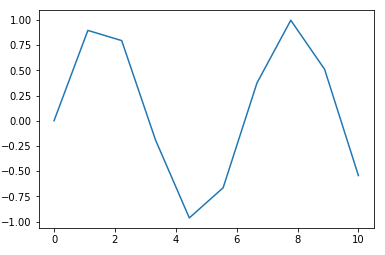
\includegraphics{Figures/ch1f1.png}
}}    
\end{center}

We end with a slightly more advanced plot, showing how to change line style and markers, and add axes labels and a legend. The NumPy \textit{cos} function takes the cosine of the array, and \textit{xlabel}, \textit{ylabel} and \textit{legend} are all Matplotlib commands to add labels to the axes and a legend to the graph.

\begin{center} {t}
\begin{lstlisting}[language=Python, frame=single]
n = 25
x = np.linspace(0, 10,25)
y = np.cos(x)
plt.plot(x, y, 'r')
x = np.linspace(0,10,5)
y = 0.01*x**2
plt.plot(x,y,'bo--')
plt.xlabel('Time')
plt.ylabel('Amplitude')
plt.legend(['Cosine', 'Quadratic'])
\end{lstlisting}
\fbox{
    \parbox{\textwidth - 2 \fboxsep}{
    Output: \\
    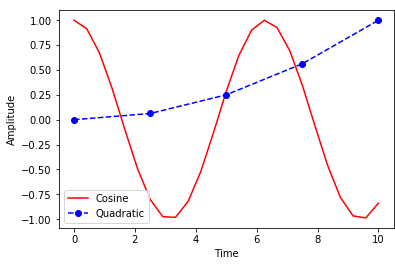
\includegraphics{Figures/ch1f2.png}
}}   
\end{center}

% SECTION: EXERCISES
\section{Exercises}

\begin{enumerate}
    \item Write a program that prints each number from 1 to 20 on a new line. For each multiple of 3, print "Fizz" instead of the number. For each multiple of 5, print "Buzz" instead of the number. For numbers which are multiples of both 3 and 5, print "FizzBuzz" instead of the number. The correct answer is: 1 2 Fizz 4 Buzz Fizz 7 8 Fizz Buzz 11 Fizz 13 14 FizzBuzz 16 17 Fizz 19 Buzz.
    
    \item Write a function to convert an angle from degrees to radians or from radians to degrees. The function should accept two inputs: the angle, and a flag to tell the function whether the angle should be converted from degrees to radians (flag = 1) or from radians to degrees (flag = 2).
    
    \item Given two 3 $\times$ 3 matrices \textbf{A} = [ [1, 2, 3], [4, 5, 6], [7, 8, 9] ] and \textbf{B} = [ [5, 7, 2], [3, 5, 1], [2, 4, 3] ], compute: 
    \begin{enumerate}
    \item  the sum of the matrices (\textbf{A} + \textbf{B}), 
    \item  The difference of the matrices (\textbf{A} - \textbf{B}), 
    \item  The product of the matrices (\textbf{AB}), 
    \item  The square root of matrix \textbf{A}, 
    \item  The sum of all elements of matrix \textbf{B}, 
    \item  The column sum of matrix \textbf{A}, 
    \item  The row sum of matrix \textbf{A}, 
    \item  The transpose of matrix $\textbf{A}\, (\textbf{A}^T)$, 
    \item  The product $\textbf{AA}^T$. What is this product equal to?
    \end{enumerate} 
    
    \textit{Hint}: Look at the functions \textit{add, subtract, dot, sqrt, sum} and \textit{transpose} in the NumPy library. 
    
    \item The apparent dip $\alpha$ of a plane is given by the following equation:
    
    \begin{equation}
        \tan\alpha=\tan\delta\sin\beta
    \end{equation}
    
    where $\delta$ is the true dip of the plane, and $\beta$ is the structural bearing (Fig. \ref{fig:strikedip}b). We will talk about this equation in chapter 3. 
    
    \begin {enumerate}
    \item Make a function to compute the apparent dip $\alpha$ from the true dip $\delta$ and structural bearing $\beta$. 
    \item Use this function in a notebook to make a graph of apparent dip $\alpha$ (0 to 90\degree, vertical axis) versus the structural bearing $\beta$ (0 to 90\degree, horizontal axis), for values of true dip $\delta$ of 10, 20, 30, 40, 50, 60, 70, and 80\degree. 
    \end{enumerate}
    
    The graph should look like the figure below:
    
    \begin{figure}[H]
        \centering
        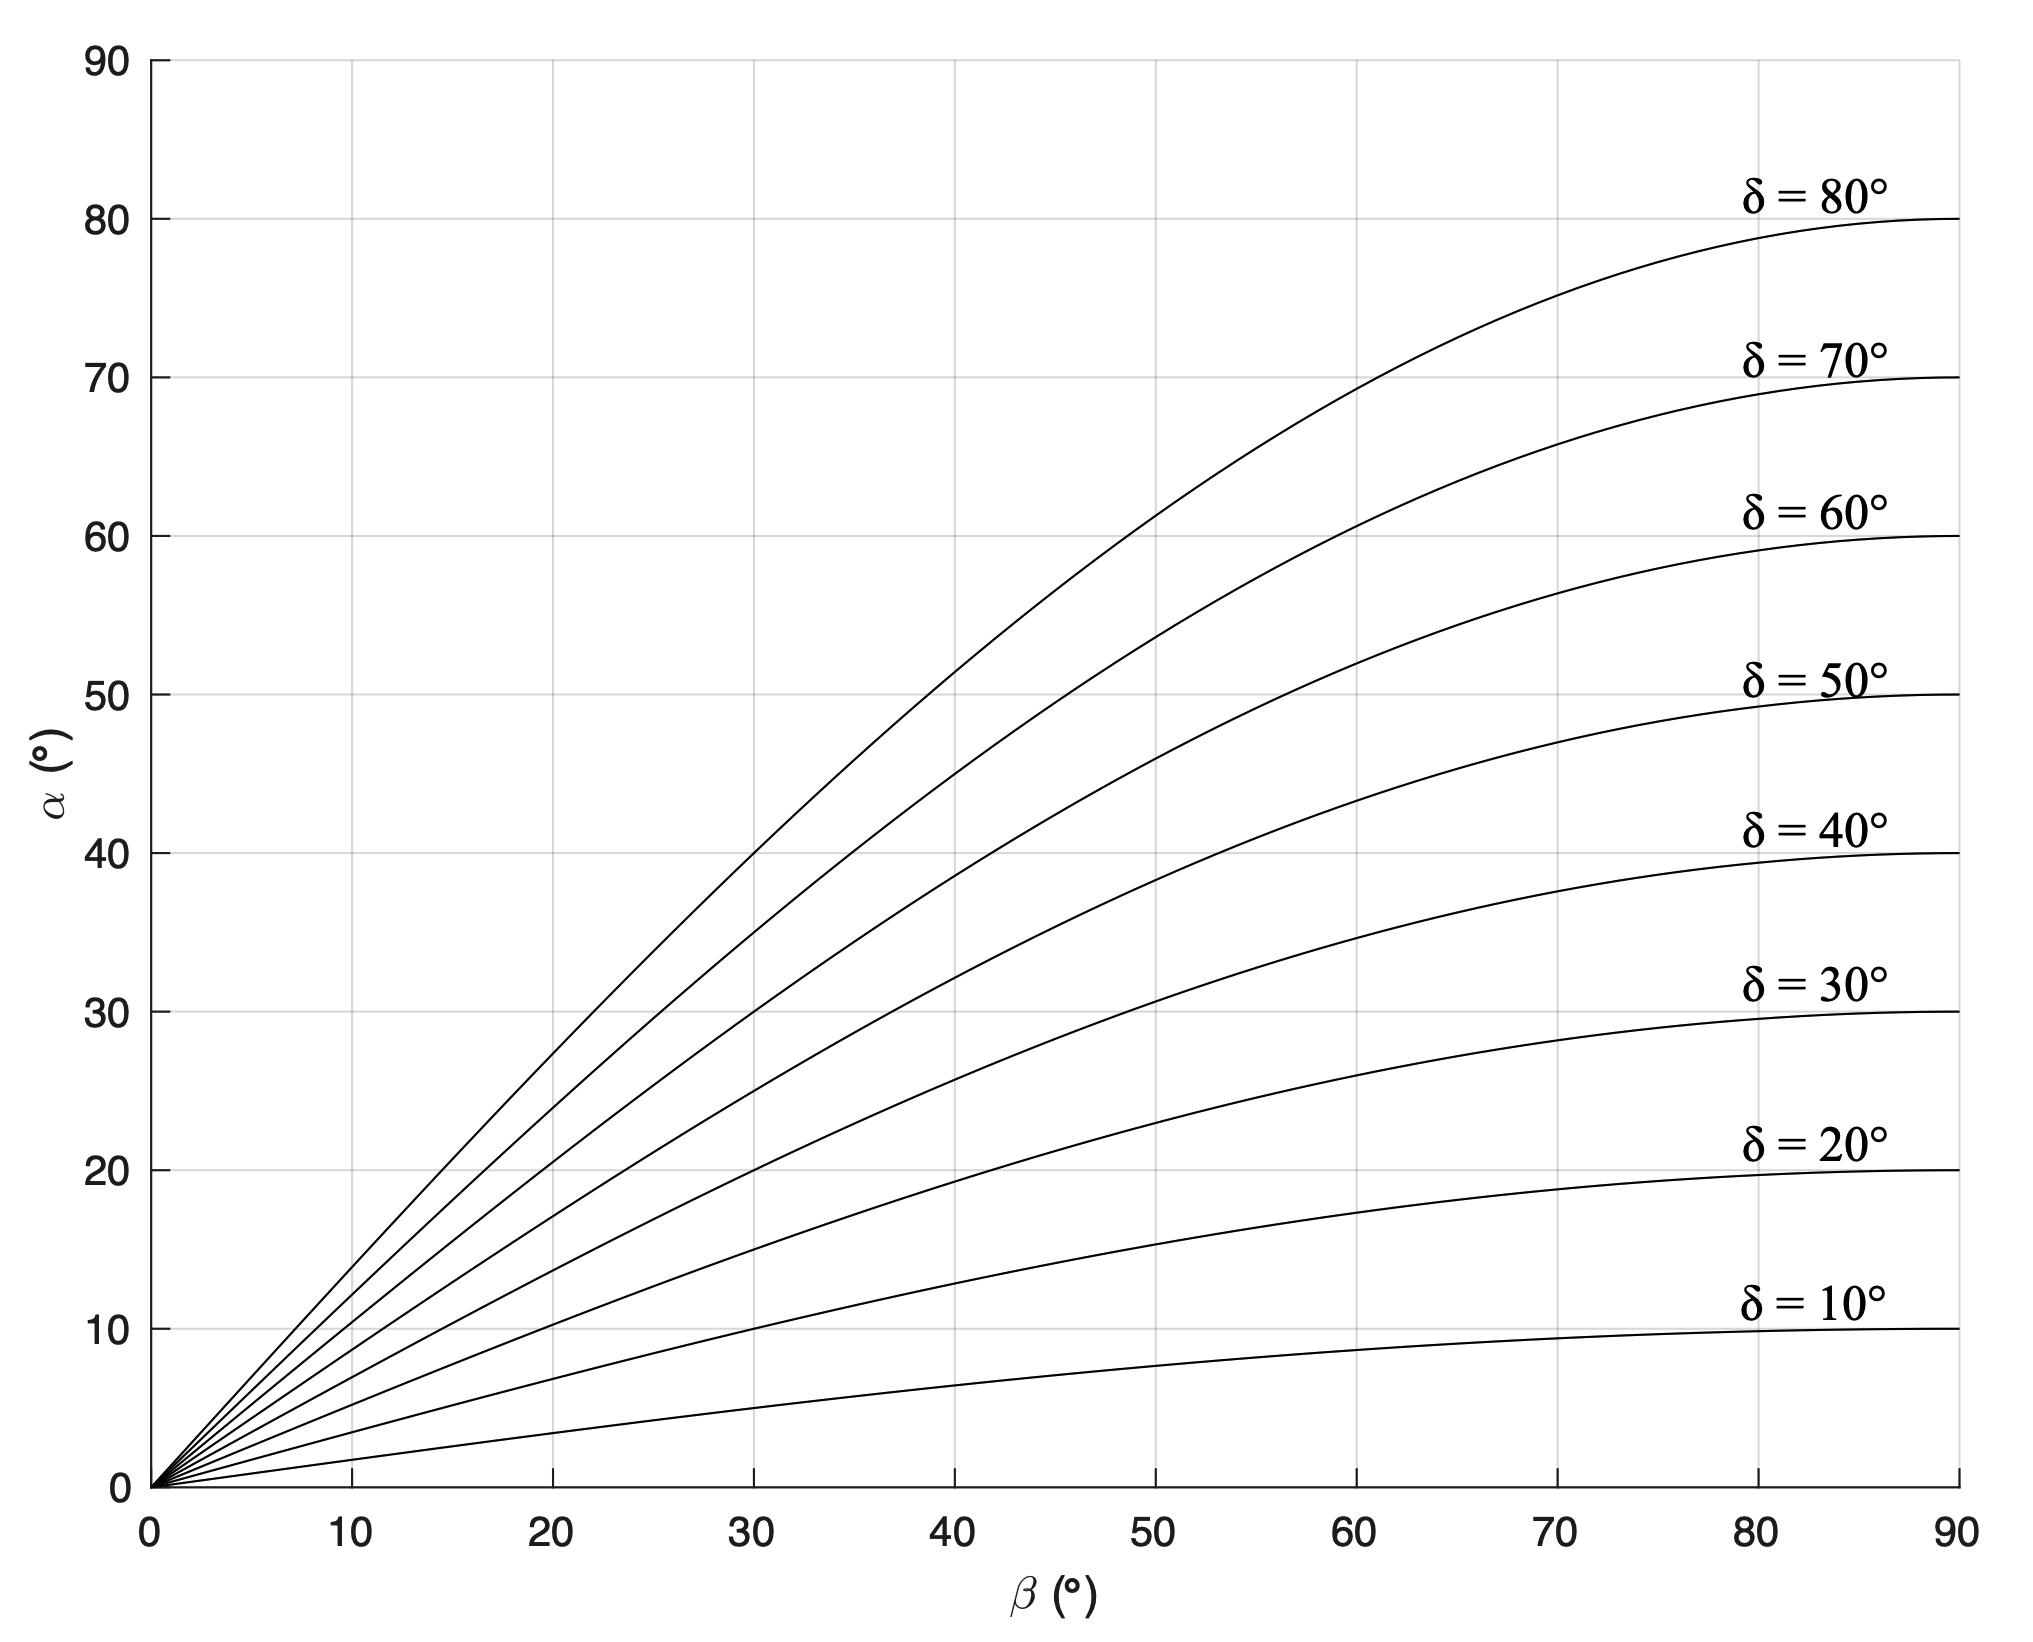
\includegraphics[width=12cm]{Figures/ch1f3.png}
        \caption{Apparent dip $\alpha$ as function of section bearing $\beta$ and true dip $\delta$}
        \label{fig:apparentdip}
    \end{figure}
\end{enumerate}

\addcontentsline{toc}{section}{References}
\section*{References}

Allmendinger, R.W., Cardozo, N. and Fisher, D.W. 2012. Structural Geology Algorithms: Vectors and Tensors. Cambridge University Press, 302 p.

Frodeman, R. 1995. Geological reasoning: Geology as an interpretive and historical science. GSA Bulletin 107, 960-968.

Jacobs, C.T., Gorman, G.J., Rees, H.E. and Craig, L.E. 2016. Experiences with efficient methodologies for teaching computer programming to geoscientists. Journal of Geological Education 64, 183-198.

Ragan, D.M. 2009. Structural Geology: An Introduction to Geometrical Techniques. Cambridge University Press, 632 p.

% CHAPTER 2: UNDERSTANDING LOCATION
\chapter{Understanding location}

% SECTION: LOCATIONS: HOW DO WE KNOW WHERE WE ARE?
\section{Locations}

Understanding where we are located or where an object of interest is located is extremely important in geosciences. Geographic information science is the study of geographic information; it includes theory and concepts and provides methods to combine and analyze spatial data (Watson, 2017). Geographic information systems is the software and technology that supports the application of geographic information theory (Watson, 2017). GIS is an acronym used for either geographic information systems or geographic information science. 

Geosciences are Earth-based and so location-based. The geographic aspect is highly applicable for the geosciences. The basic usage of GIS is cartographic – making maps. In this chapter, you will become familiar with some of the basic concepts in defining locations on the Earth. These concepts are also used for defining locations on other planets as well.

% SECTION: GEODESY BASICS
\section{Geodesy basics}

Geodesy is “the branch of mathematics dealing with the shape and area of the Earth or large portions of it” (Lexico, 2019); however, the discipline is expanding to include other planets. We need geodesy to model the Earth and make calculations because the Earth is not a perfect sphere nor flat.

\subsection{Scales}

In cartography, we use scales to describe how the real world length has been reduced to fit on a page or screen. Usually, map scales are described as ratios, such as 1:50,000. When we describe the scale, we say it is either small or large. The description of small or large refers to the scale, not the size of the area. Therefore, if we describe a scale as small, it means the fraction described by the scale ratio is small; this in turn means the map covers a large area. The inverse is true for large scales; the fraction described by the scale is large and in turn covers a small area (Kraak and Ormeling, 2003, Lisle et al., 2011). There is not an official categorical differentiation between small and large scales. Generally speaking, small scale maps cover regions, countries, and continents, while large scale maps cover neighborhoods, towns, or counties. The following example illustrates this.

\subsection*{Example 1: Understanding Map Scales}

A map has a scale of 1:1,000,000. Would you refer to this as a small or large scale?

\begin{enumerate}
    \item First, rewrite this as a fraction: 1/1,000,000
    \item Is this a small fraction or a large fraction? This is a relatively small fraction, so it is a small scale. 
\end{enumerate}

Figure 2.1 is an example of a map with a scale of 1:1,000,000.

\begin{figure}[ht]
    \centering
    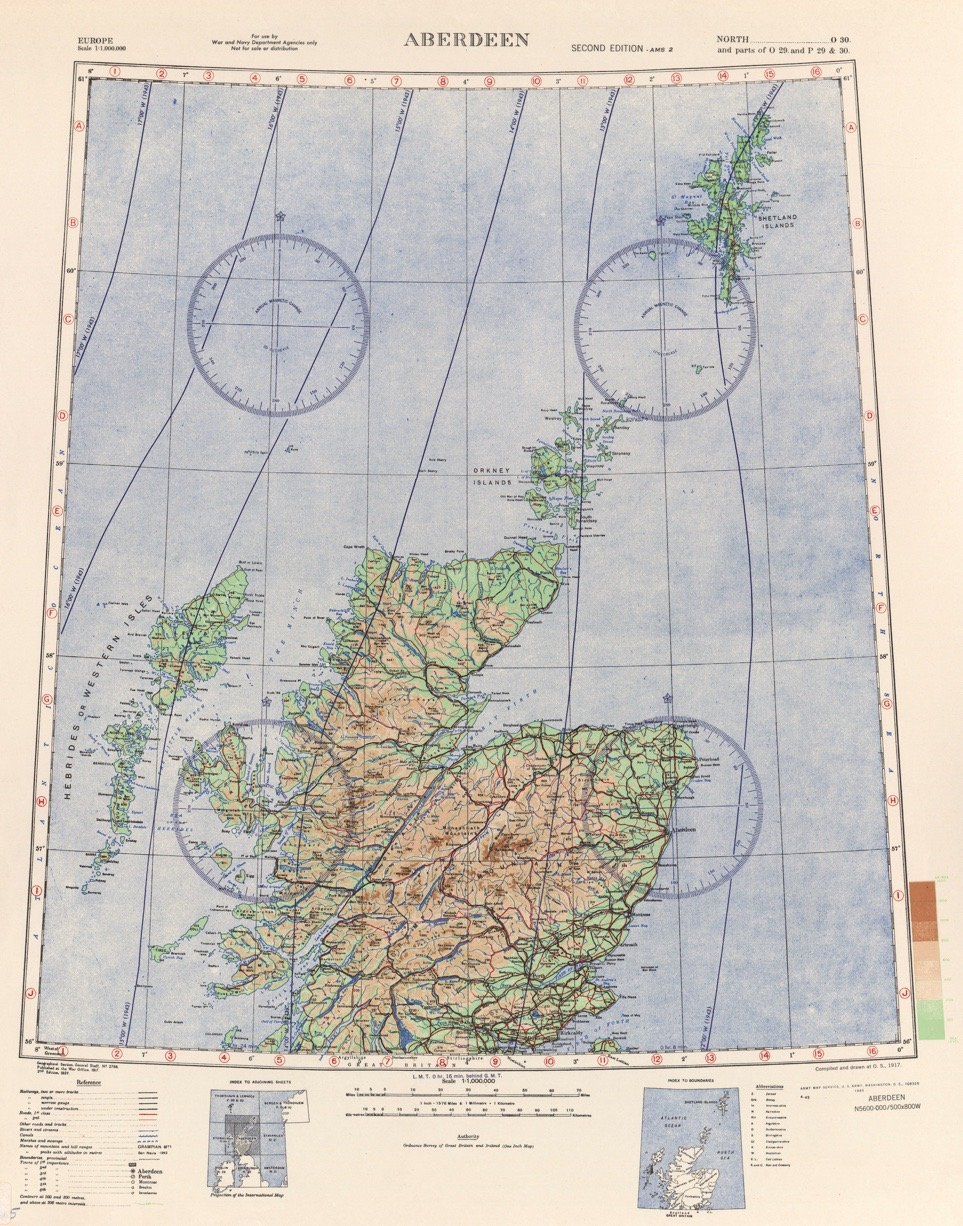
\includegraphics[width=10cm]{Figures/ch2f1.jpg}
    \caption{A historical map of northern Scotland at the scale of 1:1,000,000 (Geographic Section - General Staff, 1941).}
\end{figure}

A map has a scale of 1:10,000. Would you refer to this as a small or large scale?

\begin{enumerate}
    \item First, rewrite this as a fraction: 1/10,000
    \item Is this a small fraction or a large fraction? This is a relatively large fraction, so it is a large scale. 
\end{enumerate}

Figure 2.2 is an example of a map with a scale of 1:10,000.

\begin{figure}[ht]
    \centering
    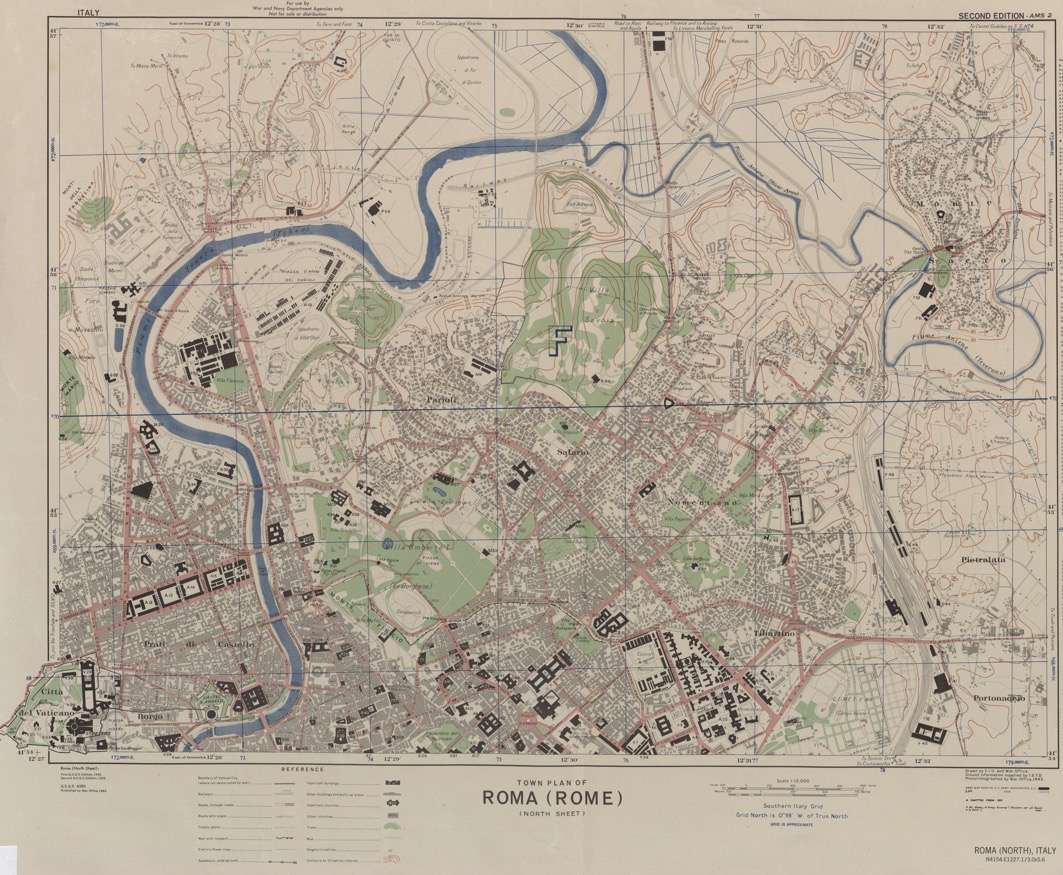
\includegraphics[width=12cm]{Figures/ch2f2.jpg}
    \caption{A historical map of Rome, Italy at the scale of 1:10,000 (C.I.U. and War Office, 1944).}
\end{figure}

\subsection{Authalic Sphere}

The authalic sphere is a sphere used for the basic surface for mapping (Fig. 2.3); its surface area is the same as the ellipsoid (Robinson et al., 1995). Based on the WGS-84 ellipsoid, the Earth has a radius of 6371 km and a circumference of 40,030.2 km. The radius is an often-used constant in geodesy (Robinson et al., 1995). The authalic sphere is used in small scale mapping (small scale covers a large area) because the difference between the authalic sphere and the ellipsoid is minimum over large areas (Robinson et al., 1995).

\begin{figure}[ht]
    \centering
    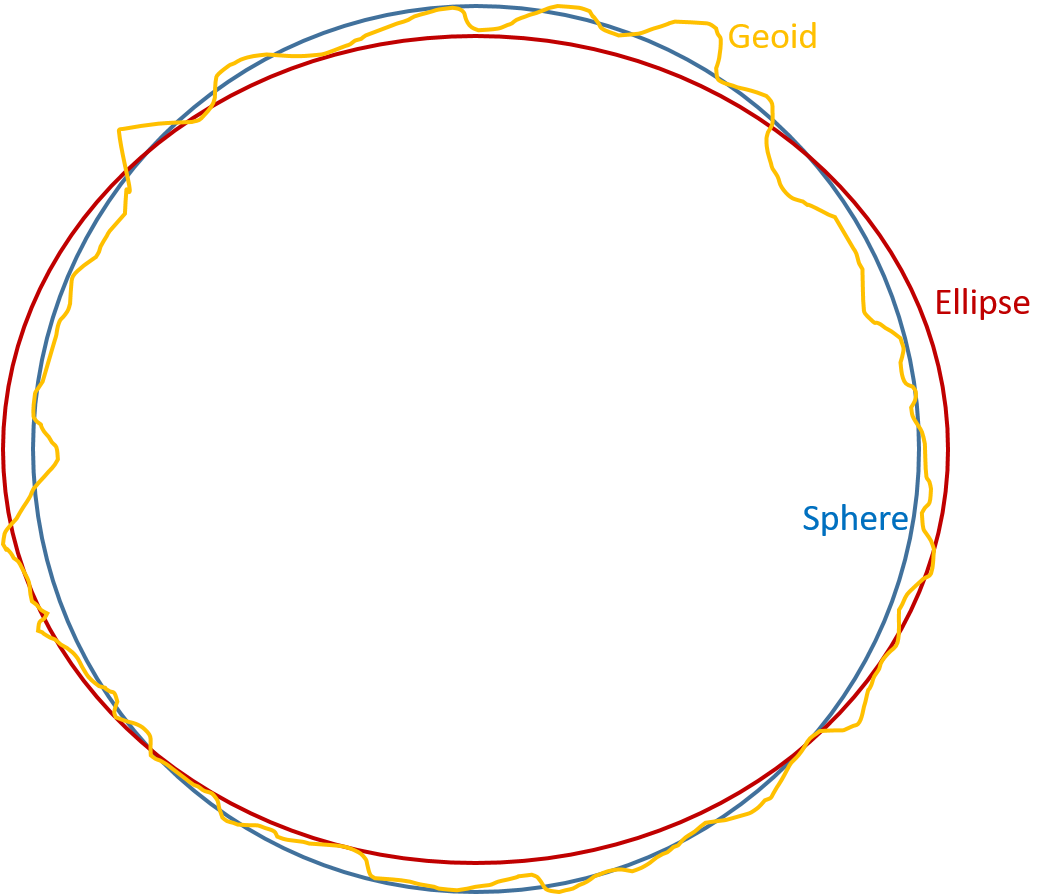
\includegraphics[width=9cm]{Figures/ch2f3.png}
    \caption{Highly stylized comparison of sphere, ellipse, and geoid.}
\end{figure}

\subsection{Ellipsoidal Earth}

Due to gravity, the Earth flattens at the poles. In a cross-section, the Earth looks like an oblate ellipsoid (Fig. 2.3) (Robinson et al., 1995). Oblateness refers to flatness. When mapping over small areas (large scale mapping), the oblateness of the ellipsoid must be taken into account. The GPS network uses the WGS-84 ellipsoid (Robinson et al., 1995).

There are varying ellipsoidal measurements on different continents and times. These continental differences are due to gravity. Temporal differences are due to technological accuracy. The WGS-84 ellipsoid is based on satellite observations and is accepted as being highly accurate (Robinson et al., 1995).

\subsection{Geoid}

Geoid means Earth-like and is in 3D. It is based on the equipotential gravity surface. The geoid follows the mean sea level in oceans and hypothetical sea-level canals on the continents (Robinson et al., 1995). Due to geology (rock density) and topography, the geoid deviates from the ellipsoid (Fig. 2.3). The geoid is a “reference surface for ground surveyed horizontal and vertical positions” (Robinson et al., 1995).

% SECTION: PROJECTIONS
\section{Projections} \label{projections}

A projection is a mathematical equation to transfer a region, of whatever size, of the round Earth onto a flat surface. Projections are used because distance and surface area calculations are more difficult on a sphere. A flat map can show greater detail than a sphere and is more transportable. Imagine how large a globe you would need to sufficiently show the streets in your neighborhood! We need projections to transform our 3D ellipsoidal Earth onto a flat map. Projections may be based on the authalic sphere, ellipsoid, or geoid.

Before proceeding, take a moment to look over an informational \href{https://pubs.usgs.gov/gip/70047422/report.pdf}{pictographic} by the U.S. Geological Survey describing different types of projection.

\subsection{Distortions}

All projections have distortions that vary by projection type (i.e. transverse Mercator vs. Miller cylindrical – see pictograph mentioned in previous section). Selecting a projection depends on discipline, size of area, orientation of area, regional standards, map purpose, and map scale. There are many resources for determining which projection you should use. Large-scale mapping uses conformal projection because angles measured on the ground are the same as those in the map (Iliffe and Lott, 2008). Four types of distortion are: area, shape, direction, and distance. The Tissot’s Indicatrix is a graphic device to show the distortion at a point (Robinson et al., 1995). We will investigate this phenomenon using the Python library \href{https://scitools.org.uk/cartopy/docs/latest/#}{Cartopy}. To install this library, follow the steps below:

\subsection*{Installing Cartopy}

We will use the Cartopy library to visualize projection distortions using the Tissot’s Indicatrix. We will make a special Cartopy Environment in Anaconda. This is because Cartopy dependencies are lower than some other libraries we’ll be using. This happens from time to time when we use open-source libraries.

\begin{enumerate}
    \item Open Anaconda Navigator.
    \item In the left panel, click on “Environments”.
    \item In the middle panel, click "Create" to create a new environment
    \item Name this environment: ch2cartopy
    \item Select Python version 3.7
    \item Click "Create". This will take a few minutes.
    \item We need to install Cartopy. In the right panel in the search field, type: cartopy
    \item You will get the message "0 packages available matching cartopy" since Cartopy is not installed.
    \item In the right panel, change "Installed" to "Not installed"
    \item Cartopy now shows up\footnote{If cartopy does not show up, you may need to press "Update index" in the right panel.}. Click the check box next to "cartopy".
    \item In the screen lower right corner, click "Apply"
    \item Please wait while Cartopy is collected and then click "Apply"
    \item The Cartopy library and any dependencies will be installed or updated. This may take a few minutes.
    \item Click on "Home"
    \item Install the console of your choice for the new environment. Click on "Install" under Jupyter Notebook, for example.
    \item Click on "Launch"
\end{enumerate}

\subsection*{Example 2: Tissot's Indicatrix}

This example will introduce you to understanding distortions in projections. As you change the projection name, a different mathematical equation will be used to portray the round Earth in a flat presentation. Pay particular attention to the size, shape, and spacing of the ellipses describing the distortion. The Tissot’s Indicatrix quickly and easily visualizes the changes in area and spatial relationships between different projections.

The notebook \href{https://github.com/nfcd/compGeo/blob/master/source/notebooks/ch2-1.ipynb}{ch2-1} contains this example. If you just launched Jupyter Notebook as indicated above, open the notebook. If you closed Anaconda, follow these steps:

\begin{enumerate}
    \item Open Anaconda Navigator
    \item Click on "Environments"
    \item Choose "ch2cartopy"
    \item Click "Home"
    \item Launch Jupyter Notebook
    \item Open the notebook ch2-1
\end{enumerate}{}

This example starts with the Plate Carree projection (\href{https://scitools.org.uk/cartopy/docs/latest/gallery/tissot.html}{Cartopy, 2018b}). Run the code below:

\begin{center}
\begin{lstlisting}[language=Python, frame=single]
import cartopy.crs as ccrs
import matplotlib.pyplot as plt

# Hide warnings
import warnings
warnings.simplefilter('ignore')

# Figure
fig = plt.figure(figsize=(10, 5))

# Plate Carree projection
ax = fig.add_subplot(1, 1, 1, projection=ccrs.PlateCarree())

# Make the map global rather than have it zoom in to
# the extents of any plotted data
ax.set_global()

# Earth image
ax.stock_img()
# Coastlines
ax.coastlines()

# Tissot's indicatrix: Orange ellipses
ax.tissot(facecolor='orange', alpha=0.4)

plt.show()
\end{lstlisting}
\fbox{
\parbox{\textwidth - 2 \fboxsep}{
Output: \\
    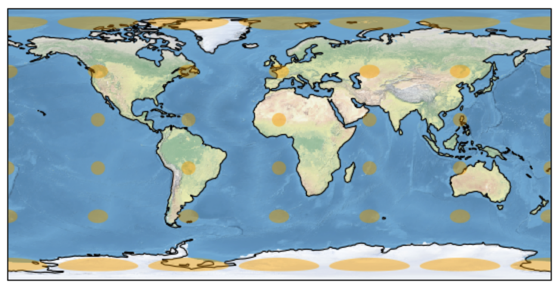
\includegraphics{Figures/ch2f4.png}
}}   
\end{center}

The Tissot’s Indicatrix is symbolized by the orange ellipses. Closer to the poles, the ellipses become more oblate; while closer to the Equator, they are more circular. The Plate Carrée projection is a specific form of the Equidistant Cylindrical projection. Plate Carrée has the latitude of origin at the Equator.

Change the code to use the Mollweide projection:

\begin{center}
\begin{lstlisting}[language=Python, frame=single]
# Figure
fig = plt.figure(figsize=(10, 5))

# Mollweide projection
ax = fig.add_subplot(1, 1, 1, projection=ccrs.Mollweide())

# Make the map global rather than have it zoom in to
# the extents of any plotted data
ax.set_global()

ax.stock_img()
ax.coastlines()

ax.tissot(facecolor='orange', alpha=0.4)

plt.show()
\end{lstlisting}
\fbox{
\parbox{\textwidth - 2 \fboxsep}{
Output: \\
    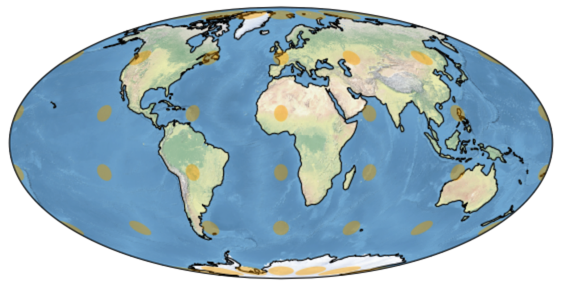
\includegraphics{Figures/ch2f5.png}
}}   
\end{center}

Notice how the sizes of the ellipses are very similar throughout the map. All of the ellipses are more rounded and circular regardless of their position, as compared to the Plate Carrée projection. Mollweide is often used for world maps.

Cartopy has a list of projections that are included in the library  (\href{https://scitools.org.uk/cartopy/docs/latest/crs/projections.html}{Cartopy, 2018a}). Change the code above to project the map in Azimuthal Equidistant. 

% SECTION: COORDINATE REFERENCE SYSTEMS AND DATUMS
\section{Reference systems and datums}

A coordinate reference system is a coordinate system that has been referenced to a datum. A datum is the location used for a reference point from which spatial measurements are made. There are geographic and Cartesian coordinate systems. Coordinates are for specific locations on the Earth. They can be expressed as geographic using latitude and longitude. Latitude are parallels that are evenly spaced and longitude are meridians that converge at the poles. These are measured in degrees. Cartesian coordinates are expressed in x and y and may have units that are meters, feet, or kilometers, for example. Coordinates only have meaning when the coordinate system and datum are known (Iliffe and Lott, 2008, Robinson et al., 1995). 

\subsection*{Example 3: Defining the coordinate reference system}

In any GIS program, including spatial libraries and code, the user must ensure that the coordinate reference system is defined for the spatial data. The GIS software will make assumptions, sometimes erroneous, if the coordinate reference system is not properly defined. In this example, we will see a demonstration of these assumptions and how to prevent them. This example is from the SciTools tutorials to understand Cartopy (\href{https://scitools.org.uk/cartopy/docs/latest/tutorials/understanding_transform.html}{Cartopy, 2018c}).

In Cartopy, there are two keywords that you must understand in order to properly display your data. The “projection” argument is used for display of your data. This only affects the map or plot. It does not define the coordinate reference system of the data itself. The “transform” argument, on the other hand, defines the coordinate reference system. The best practice is to define both of these. We will investigate the error that occurs when the best practice is not followed and compare this to when the best practice is followed. The notebook \href{https://github.com/nfcd/compGeo/blob/master/source/notebooks/ch2-2.ipynb}{ch2-2} contains this example.

First we will create some dummy data on a regular latitude/longitude grid:\\

\begin{center}
\begin{lstlisting}[language=Python, frame=single]
import numpy as np

lon = np.linspace(-80, 80, 25)
lat = np.linspace(30, 70, 25)
lon2d, lat2d = np.meshgrid(lon, lat)

data = np.cos(np.deg2rad(lat2d) * 4) + np.sin(np.deg2rad(lon2d) * 4)
\end{lstlisting}
\end{center}

In order to demonstrate the error before "best practice", we will create a map using the Plate Carree projection but only specify the "projection" argument. Remember that the best practice requires both projection and transform arguments to be defined.

\begin{center}
\begin{lstlisting}[language=Python, frame=single]
import cartopy.crs as ccrs
import matplotlib.pyplot as plt

# The projection keyword determines how the plot will look
plt.figure(figsize=(6, 3))
ax = plt.axes(projection=ccrs.PlateCarree())
ax.set_global()
ax.coastlines()

# didn't use transform, but looks ok...
ax.contourf(lon, lat, data)  
plt.show()
\end{lstlisting}
\fbox{
\parbox{\textwidth - 2 \fboxsep}{
Output: \\
    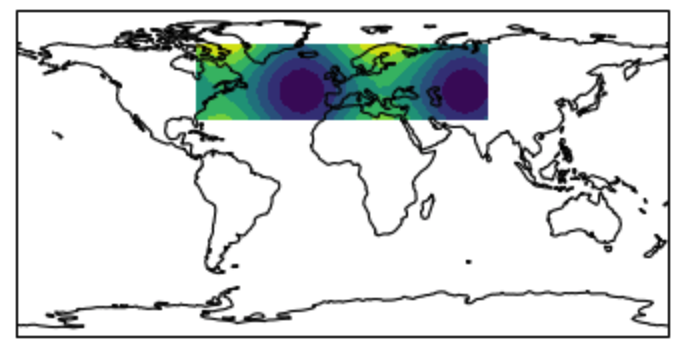
\includegraphics[width=10cm]{Figures/ch2f6.png}
}}   
\end{center}

In this case, the data just happen to fall in the correct location. Now, we will define the data coordinate reference system (first line of code below) and add the transform argument to the plot (second last line of code below).

\begin{center}
\begin{lstlisting}[language=Python, frame=single]
# The data are defined in lat/lon coordinate system, 
# so PlateCarree() is the appropriate choice:
data_crs = ccrs.PlateCarree()

# The projection keyword determines how the plot will look
plt.figure(figsize=(6, 3))
ax = plt.axes(projection=ccrs.PlateCarree())
ax.set_global()
ax.coastlines()

# use transform
ax.contourf(lon, lat, data, transform=data_crs) 
plt.show()
\end{lstlisting}
\fbox{
\parbox{\textwidth - 2 \fboxsep}{
Output: \\
    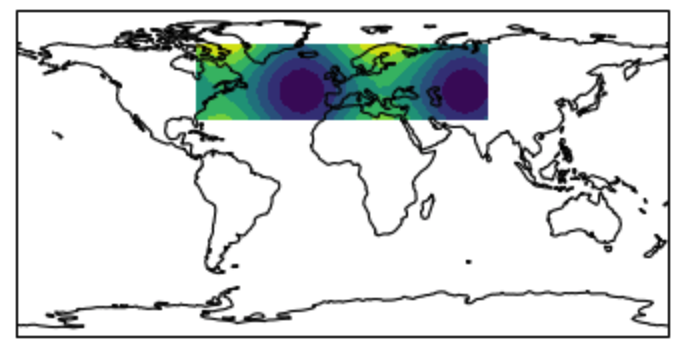
\includegraphics[width=10cm]{Figures/ch2f6.png}
}}   
\end{center}

You will notice that our plot remains unchanged. The assumption, as stated previously, is that if the coordinate reference system of the data is undefined, it is the same as the map (or plot) projection. In the example above, this has been the case. Let us now investigate what happens when changing the projection of the map without defining the coordinate reference system of the data. We now define the projection to "RotatedPole" and omit the transform argument to see what happens:

\begin{center}
\begin{lstlisting}[language=Python, frame=single]
# Now we plot a rotated pole projection
projection = ccrs.RotatedPole(pole_longitude=-177.5, pole_latitude=37.5)
plt.figure(figsize=(6, 3))
ax = plt.axes(projection=projection)
ax.set_global()
ax.coastlines()

ax.contourf(lon, lat, data)  # didn't use transform, uh oh!
plt.show()
\end{lstlisting}
\fbox{
\parbox{\textwidth - 2 \fboxsep}{
Output: \\
    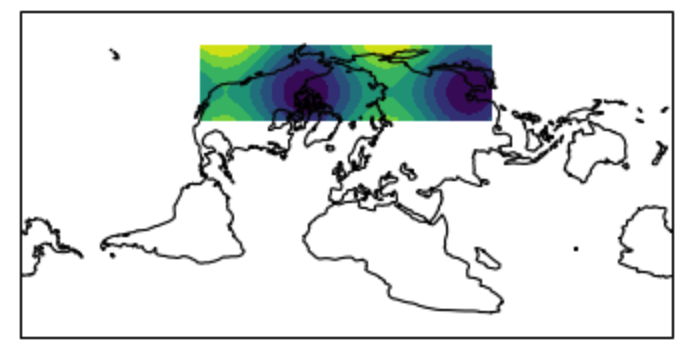
\includegraphics[width=10cm]{Figures/ch2f7.png}
}}   
\end{center}

In this case, we see that the country boundaries have rotated and changed shape, however, the data did not move with the the country boundaries. We made a wrong assumption in the data definition. Therefore we need to define the transform argument:

\begin{center}
\begin{lstlisting}[language=Python, frame=single]
# A rotated pole projection again...
projection = ccrs.RotatedPole(pole_longitude=-177.5, pole_latitude=37.5)
plt.figure(figsize=(6, 3))
ax = plt.axes(projection=projection)
ax.set_global()
ax.coastlines()

# ...but now using the transform argument
ax.contourf(lon, lat, data, transform=data_crs)
plt.show()
\end{lstlisting}
\fbox{
\parbox{\textwidth - 2 \fboxsep}{
Output: \\
    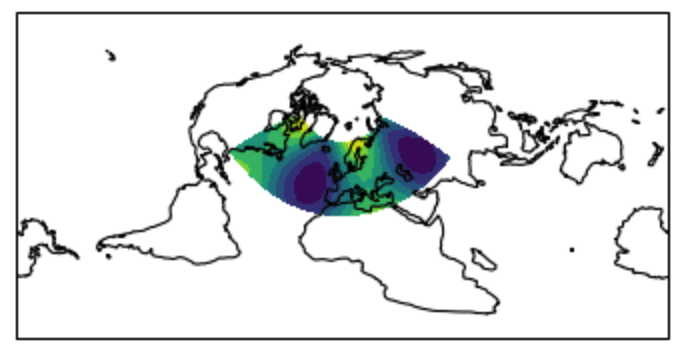
\includegraphics[width=10cm]{Figures/ch2f8.png}
}}   
\end{center}

Now the data are correctly projected. Get in the habit of always defining the coordinate reference system and the map plot projection. It will save headaches and misunderstandings of the data.

Here is another script using an entirely different projection and additional plotting parameters. Can you figure out what the script will produce before running the cell? Notice the presence of the Matplotlib function \textit{subplot}. What do you think this function does?

\begin{center}
\begin{lstlisting}[language=Python, frame=single]
# We can choose any projection we like...
projection = ccrs.InterruptedGoodeHomolosine()
plt.figure(figsize=(6, 7))
ax1 = plt.subplot(211, projection=projection)
ax1.set_global()
ax1.coastlines()
ax2 = plt.subplot(212, projection=ccrs.NorthPolarStereo())
ax2.set_extent([-180, 180, 20, 90], crs=ccrs.PlateCarree())
ax2.coastlines()

# ...as long as we provide the correct transform, 
# the plot will be correct
ax1.contourf(lon, lat, data, transform=data_crs)
ax2.contourf(lon, lat, data, transform=data_crs)
plt.show()
\end{lstlisting}
\end{center}

Now that you have worked through the exercise, you should have an understanding of why it is important to fully define the coordinate reference system and the projection when creating a map.

% SECTION: COORDINATE CONVERSION AND TRANSFORMATION
\section{Conversion vs. transformation}

When working with data collected from several sources or in different coordinate reference systems, the data must be redefined to have the same coordinate reference system and datum. Consistent coordinate reference systems for data in a map is important because there may be spatial differences between the coordinate reference systems creating locational errors. A coordinate conversion is when the coordinate reference systems have the same datum. A coordinate transformation is when the coordinate reference systems have different datums.

When making a map, all of the data in the map should have the same coordinate reference system definition. Software include many definitions and transformations but refer to Snyder (1987) and International Association of Oil and Gas Producers (2018) for projection formulae (Iliffe and Lott, 2008). In Example 2, the Tissot’s Indicatrix ellipses did not change coordinate reference systems. The method used to plot the ellipses changed. In Example 3, we also only changed the projection of the map, not the coordinate reference system. In the following examples, we will make coordinate conversions and transformations. For this purpose, we will use the \href{https://pypi.org/project/pyproj/}{pyproj} Python library and examples from the pyproj documentation (\href{https://pyproj4.github.io/pyproj/stable/api/transformer.html?highlight=transformer}{Whitaker, 2019}).

\subsection*{Installing pyproj}

A version of pyproj was installed with Cartopy, but you need the latest version which has different dependencies than Cartopy. You will create a new environment.

\begin{enumerate}
    \item Open Anaconda Navigator.
    \item In the left panel, click on "Environments"
    \item In the middle panel, click "Create" to create a new environment
    \item Name this environment: ch2pyproj
    \item Select Python version 3.7
    \item Click "Create". This will take a few minutes
    \item We need to install pyproj. In the right panel in the search field, type: pyproj
    \item You will get the message "0 packages available matching pyproj" since pyproj is not installed. 
    \item In the right panel, change "Installed" to "Not installed"
    \item pyproj now shows up. Click the check box next to "pyproj".
    \item In the screen lower right corner, click "Apply"
    \item Please wait while pyproj is collected and then click "Apply"
    \item The pyproj library and any dependencies will be installed or updated. This may take a few minutes.
    \item Click on "Home"
    \item Install the console of your choice for the new environment. Click on "Install" under Jupyter Notebook, for example.
    \item Click on "Launch"
\end{enumerate}

\subsection*{Example 4: Coordinate conversion}

The notebook \href{https://github.com/nfcd/compGeo/blob/master/source/notebooks/ch2-3.ipynb}{ch2-3} contains this example. If you just launched Jupyter Notebook as indicated above, open the notebook. If you closed Anaconda, follow these steps:

\begin{enumerate}
    \item Open Anaconda Navigator
    \item Click on "Environments"
    \item Choose "ch2pyproj"
    \item Click "Home"
    \item Launch Jupyter Notebook
    \item Open the notebook ch2-3
\end{enumerate}{}

We have a coordinate pair defined in decimal degrees of latitude and longitude. The longitude is -120.108\degree and latitude is 34.3611666\degree. We want to make a coordinate conversion from latitude and longitude to Universal Transverse Mercator, where the point is defined by east and north coordinates in meters. To learn more about Universal Transverse Mercator (UTM), refer to (Snyder, 1987). In the code, we use the pyproj \textit{Proj} function. We can only use \textit{Proj} when making a coordinate conversion (i.e. the same datum):

\begin{center}
\begin{lstlisting}[language=Python, frame=single]
from pyproj import Proj

# Construct the projection matrix
p = Proj(proj='utm',zone=10,ellps='WGS84', preserve_units=False)

# Apply the projection to the lat-long point
x,y = p(-120.108, 34.36116666)

print(f'x={x:9.3f}, y={y:11.3f}')
\end{lstlisting}
\fbox{
\parbox{\textwidth - 2 \fboxsep}{
Output:\\
x=765975.641, y=3805993.134
}}   
\end{center}

This is the same location but only expressed in east and north coordinates in meters using the UTM coordinate reference system. The datum used is WGS84. We can convert the UTM coordinates back to latitute and longitude by adding two lines of code:

\begin{center}
\begin{lstlisting}[language=Python, frame=single]
# Apply the inverse of the projection matrix
# to the point in UTM
lon,lat = p(x,y,inverse=True)
print(f'lon={lon:8.3f}, lat={lat:5.3f}')
\end{lstlisting}
\fbox{
\parbox{\textwidth - 2 \fboxsep}{
Output:\\
lon=-120.108, lat=34.361
}}   
\end{center}

In the two cells of code above, we’ve truncated the output to only three decimal places, but we can confirm that the inverse conversion arrives at the original pair. Let's now try converting several points of different latitude and longitude using a collection of objects in Python, or tuples. Add the following code:

\begin{center}
\begin{lstlisting}[language=Python, frame=single]
# three points in lat-long
lons = (-119.72,-118.40,-122.38)
lats = (36.77, 33.93, 37.62 )
# Apply the projection to the points
x1,y1 = p(lons, lats)
print(x1,y1)
\end{lstlisting}
\fbox{
\parbox{\textwidth - 2 \fboxsep}{
Output:\\
(792763.8631257227, 925321.5373562573, 554714.3009414743)\\ 
(4074377.6167697194, 3763936.9410883673, 4163835.3033114495)
}}   
\end{center}

Now, let's do a more advanced exercise: In the cartographic community, an easy way to communicate the coordinate reference system is to use the EPSG Geodetic Parameter Data set. Every coordinate reference system is given a code. This ensures that if someone uses UTM zone 10 North with datum WGS-84 and tells you UTM zone 10, that you do not accidentally use UTM zone 10 North with datum GRS80, for example.

Earlier in this exercise, we defined the UTM zone in the \textit{Proj} function. Here, we will refer to the EPSG code. First, we will take a coordinate pair in longitude and latitude with datum WGS84 and convert it to EPSG:32667. Before proceeding, conduct a quick internet search on what EPSG:32667 means. This is important to understand what we will do next. The first part of the code is:

\begin{center}
\begin{lstlisting}[language=Python, frame=single]
# silence warnings
import warnings
warnings.simplefilter('ignore')

# initial coordinate conversion
p = Proj(init='EPSG:32667', preserve_units=True)
# Apply the conversion to the lat-long point
x,y = p(-114.057222, 51.045)
print(f'x={x:9.3f}, y={y:11.3f} (feet)')
\end{lstlisting}
\fbox{
\parbox{\textwidth - 2 \fboxsep}{
Output:\\
x=-5851386.754, y=20320914.191 (feet)
}}   
\end{center}

Let’s dissect this as the pyproj code looks quite a bit different. The first part of the function Proj calls EPSG:32667. If you looked up EPSG:32667 online, you found that it is for UTM zone 17 North, but the units are in feet. The default mode for Proj is “preserve\textunderscore units=False”, which forces any unit to meters. However, we want to see the units in US Survey Feet as the projection defines; therefore, we change the argument to True.

Now, suppose we want to see the output in meters. How will you amend the code? Here is what you should add:

\begin{center}
\begin{lstlisting}[language=Python, frame=single]
# Print the coordinate pair in meters
p1 = Proj(init='EPSG:32667', preserve_units=False)
x1,y1 = p1(-114.057222, 51.045)
print(f'x={x1:9.3f}, y={y1:11.3f} (meters)')
\end{lstlisting}
\fbox{
\parbox{\textwidth - 2 \fboxsep}{
Output:\\
x=-1783506.250, y=6193827.033 (meters)
}}   
\end{center}

As discussed, you should change “preserve\textunderscore units=False” and change the unit to be printed from “feet” to “meters”. Congratulations! You now have a good understanding of coordinate conversion.

\subsection*{Example 5: Coordinate transformation}

We learned earlier that we have a coordinate conversion where a coordinate pair is converted between coordinate reference systems with the same datum. In many instances, the coordinate reference system will also undergo a datum shift – this is a coordinate transformation.

This example is included in the notebook \href{https://github.com/nfcd/compGeo/blob/master/source/notebooks/ch2-4.ipynb}{ch2-4}. We will use the pyproj \textit{CRS} and \textit{transform} functions. The \textit{CRS} function defines the coordinate reference system while the \textit{transform} function specifies which coordinate reference system is the original and which is the output. \textit{CRS} has the same ability to refer directly to an EPSG code.

The input coordinates are in EPSG:4327, which is a commonly used code. It is the geographic coordinate system with datum WGS84. The output coordinates are EPSG:31984, which is for UTM zone 24 S with datum SIRGAS2000.

\begin{center}
\begin{lstlisting}[language=Python, frame=single]
from pyproj import transform
from pyproj import CRS

# input coordinates
c1 = CRS('EPSG:4327')
# coordinate pair
y1=-10.754283
x1=-39.866132
# output coordinates
c2 = CRS('EPSG:31984')
# Coordinate transformation
x2, y2 = transform(c1, c2, x1, y1)
print(f'x={x2:9.3f}, y={y2:11.3f}')
\end{lstlisting}
\fbox{
\parbox{\textwidth - 2 \fboxsep}{
Output:\\
x=2930179.850, y=5185231.716
}}   
\end{center}

\subsection*{Example 6: Transforming several points at once}

We have focused our examples on one coordinate pair at a time. The reality is that you will more often have several coordinates to transform at one time. The notebook \href{https://github.com/nfcd/compGeo/blob/master/source/notebooks/ch2-5.ipynb}{ch2-5} explains how to do this.

We have a csv file with two columns: longitude and latitude. Each coordinate pair is the center of a volcano around the world. There are 1,509 volcanoes in our dataset. The original coordinate reference system is geographic coordinates with datum WGS84. We want to make a coordinate transformation of these data points to World Mercator. It will take much too long to manually transform these coordinates as we have done in the notebooks before. Therefore, our new code will read the csv file and create a new csv file.

Check that the pathway of \textit{in\textunderscore path} and \textit{out\textunderscore path} matches the directory where the csv file is. In this example, the volcanoes file (\href{https://github.com/nfcd/compGeo/blob/master/source/data/ch2-5/volc_longlat.csv}{\textit{volc\textunderscore longlat.csv}}) is in the directory \textit{data/ch2-5}. Run the code, you will know the process is finished when the message "process completed" and the time of execution are returned:

\begin{center}
\begin{lstlisting}[language=Python, frame=single]
import csv
import pyproj
from functools import partial
from os import listdir, path

# time the execution of the code
import time
start_time = time.time()


# Remove warnings
import warnings
warnings.simplefilter('ignore')

#Define some constants at the top

lon = 'LONGITUDE' #name of longitude field in original files
lat = 'LATITUDE' #name of latitude field in original files
f_x = 'x' #name of new x value field in new projected files
f_y = 'y' #name of new y value field in new projected files
in_path = path.abspath('../data/ch2-5') #input directory
out_path = path.abspath('../data/ch2-5') #output directory
input_projection = 'EPSG:4326' #WGS84
output_projection = 'EPSG:3395' #World Mercator

#Get CSVs to reproject from input path
files= [f for f in listdir(in_path) if f.endswith('.csv')]

#Define partial function for use later when reprojecting
project = partial(
    pyproj.transform,
    pyproj.Proj(init=input_projection),
    pyproj.Proj(init=output_projection))

for csvfile in files:
    #open a writer, appending '_project' onto the base name
    with open(path.join(out_path, csvfile.replace('.csv','_project.csv')), 'w') as w:
        #open the reader
        with open(path.join( in_path, csvfile), 'r') as r:
            reader = csv.DictReader(r, dialect='excel')
            #Create new fieldnames list from reader
            # replacing lon and lat fields with 
            # x and y fields
            fn = [x for x in reader.fieldnames]
            fn[fn.index(lon)] = f_x
            fn[fn.index(lat)] = f_y
            writer = csv.DictWriter(w, fieldnames=fn)
            #Write the output
            writer.writeheader()
            for row in reader:
                x,y = (float(row[lon]), float(row[lat]))
                try:
                    #Add x,y keys and remove lon, lat keys
                    row[f_x], row[f_y] = project(x, y) # project point
                    row.pop(lon, None)
                    row.pop(lat, None)
                    writer.writerow(row)
                except Exception as e:
                    #If coordinates are out of bounds, 
                    #skip row and print the error
                    print (e)
print('process completed')
end_time = time.time()
print("it took {} seconds to run the code".format(end_time-start_time))
\end{lstlisting}
\fbox{
\parbox{\textwidth - 2 \fboxsep}{
Output:\\
process completed \\
it took 55.04537224769592 seconds to run the code
}}   
\end{center}

It takes about 55 seconds to run this code in a standard computer. Check the newly created csv file and notice that you now have a listing of coordinates in meters. The EPSG definition of the output coordinate reference system is listed under \textit{output\textunderscore projection}. You can easily change this variable to another EPSG and rerun the script. Notice that the code is written so that every csv file in the directory will undergo a coordinate transformation. 

% SECTION: EXERCISES
\section{Exercises}

\addcontentsline{toc}{section}{References}
\section*{References}

C.I.U. AND WAR OFFICE. 1944. Town Plan of Roma (Rome) (North Sheet), 1:10,000. Washington, D. C.: War Office.

Cartopy. 2018a. Projections [\href{https://scitools.org.uk/cartopy/docs/latest/crs/projections.html}{Online}]. UK: SciTools. [Accessed 19 November, 2019]

Cartopy. 2018b. Tissot’s Indicatrix [\href{https://scitools.org.uk/cartopy/docs/latest/gallery/tissot.html}{Online}]. UK: SciTools. [Accessed 19 November, 2019].

Cartopy. 2018c. Understanding the Transform and Projection Keywords [\href{https://scitools.org.uk/cartopy/docs/latest/tutorials/understanding_transform.html}{Online}]. UK: SciTools. [Accessed 19 November, 2019].

Geographic Section - General Staff. 1941. Aberdeen, 1:1,000,000. Great Britain: War Office.

Iliffe, J. and Lott, R. 2008. Datums and Map Projections: For Remote Sensing, GIS, and Surveying, Dunbeath, Scotland, Whittles.

International Association of Oil and Gas Producers. 2018. Geomatics Guidance Note 7, Part 2 Coordinate conversions and Transformations including Formulas.

Kraak, M.J. and Ormeling, F.J. 2003. Cartography: visualization of geospatial data. Addison Wesley.

Lexico. 2019. Geodesy [\href{https://www.lexico.com/en/definition/geodesy}{Online}]. Oxford. [Accessed August, 2019].

Lisle, R. J., Brabham, P. and Barnes, J. W. 2011. Basic Geological Mapping, Chicester, UK, Wiley-Blackwell.

Robinson, A. H., Morrison, J. L., Muehrcke, P. C., Kimerling, A. J. and Guptill, S. C. 1995. Elements of Cartography, New York, Wiley.

Snyder, J. P. 1987. Map Projections: a working manual. Geological Survey Professional Paper. Washington, D. C., U.S.A.: United States Government Printing Office.

Watson, L. 2017. Spatial-based assessment at continental to global scale: case studies in petroleum exploration and ecosystem services. PhD, Utrecht University.

Whitaker, J. 2019. pyproj Transformer Documentation [\href{https://pyproj4.github.io/pyproj/stable/api/transformer.html?highlight=transformer}{Online}].  [Accessed 7 January, 2020].

% CHAPTER 3: GEOLOGIC FEATURES
\chapter{Geologic features}

% SECTION: PRIMITIVE OBJECTS: LINES AND PLANES
\section{Primitive objects: Lines and planes}

The fundamental geometric features of geology are lines (e.g. a lineation or a fold axis) and planes (e.g. bedding or a foliation). A \textit{line} is the element generated by a moving point. It can be straight or curved. We will treat straight lines here. A \textit{plane} is a flat surface; a line joining two points on the plane lies wholly on its surface, and two intersecting lines on the plane define the plane. This is equivalent to say that three non-collinear points on the plane define the plane (this is the principle of the well-known three-point problem). Obviously, linear features can be curved (e.g. the intersection of bedding with irregular topography), and surfaces can be non-planar (e.g. bedding on a fold). However, even these more complex cases can be expressed as a collection of lines and planes.

% SECTION: MEASURING LINES AND PLANES
\section{Lines and planes orientations}

Two important properties of lines and planes are location (chapter 2) and orientation (this chapter). Lines and planes orientations are measured with respect to the geographic north and the angle downward or upward from the horizontal. We refer to this coordinate system as the spherical coordinate system, and the measurements defining the lines or planes orientations as the spherical coordinates.

% SUBSECTION: PLANES: STRIKE AND DIP
\subsection{Planes: Strike and dip}

A plane orientation can be defined by the angle a horizontal line on the plane makes with the geographic north, known as the \textit{strike} and the maximum angle measured downward from the horizontal to the plane, known as the \textit{dip} (Fig 3.1a). The strike is measured as an azimuth, an angle between 0 and  360\degree (0 = north, 90 = east, 180 = south, 270 = west). The dip is an angle between 0 (horizontal plane) and 90\degree (vertical plane). The projection of the dip onto the horizontal is known as the \textit{dip direction} and is always 90\degree from the strike. However, is the dip direction plus or minus 90\degree the given strike? Which end of the strike line should we use? To avoid ambiguities, we will use a format known as the \textit{right hand rule} (RHR). In the RHR format, one gives the strike such that the dip direction is always the strike plus 90\degree, i.e. the dip direction is to the right of the strike (Fig. 3.1a).

\begin{figure}[ht]
    \centering
    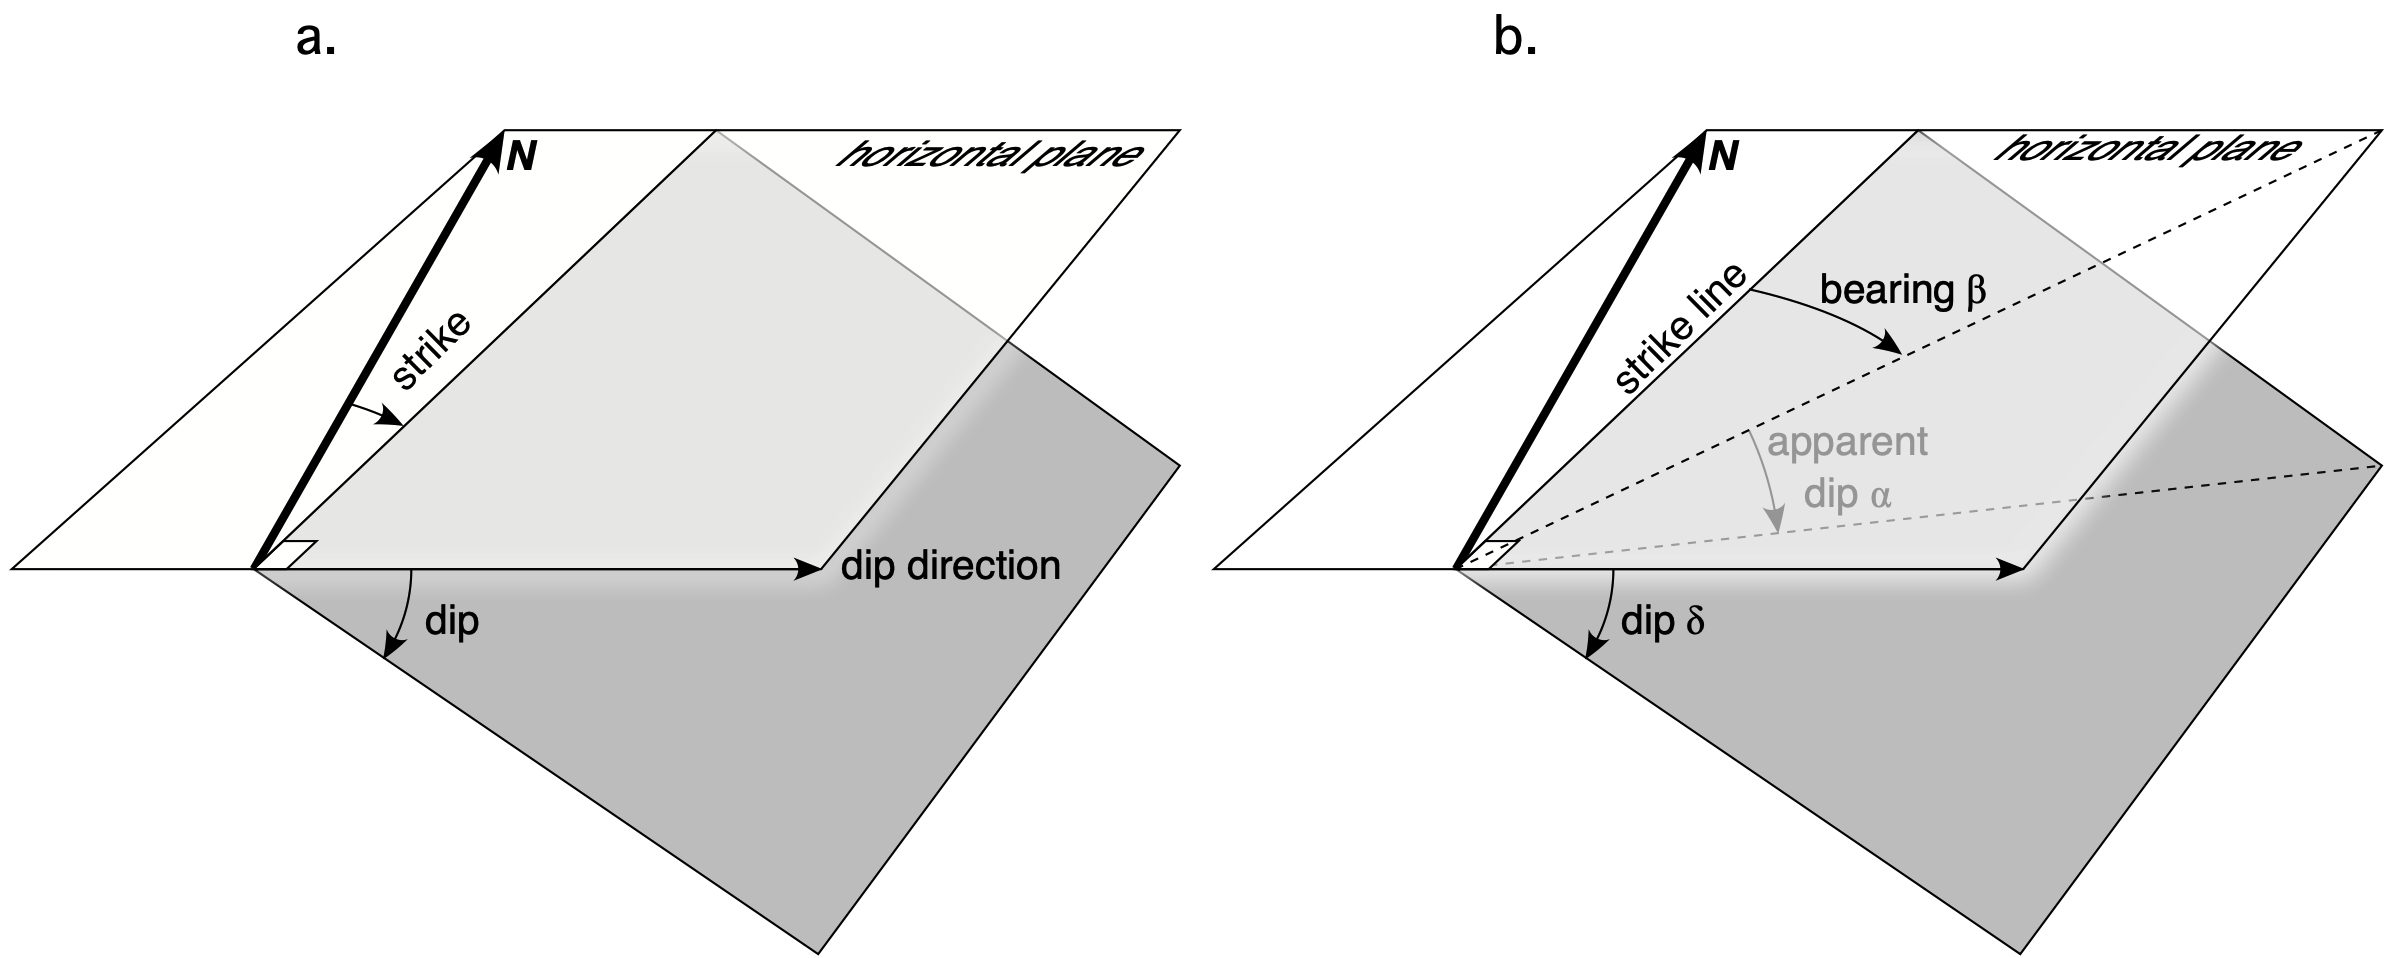
\includegraphics[width=13cm]{Figures/ch3f1.png}
    \caption{\textbf{a.} Strike and dip of a plane, \textbf{b.} Apparent dip of a plane. Modified from Allmendinger et al. (2012).}
    \label{fig:strikedip}
\end{figure}

It is only along the dip direction that the true dip can be measured, any other direction will give a lower apparent dip (Fig. 3.1b). The relation between the dip ($\delta$) and the apparent dip ($\alpha$) is given by the equation:

\begin{equation}
    \tan\alpha=\tan\delta\sin\beta
\end{equation}

where $\beta$ is the angle between the strike (horizontal) line on the plane and the vertical section on which the apparent dip is measured (Fig. 3.1b). This is also Eq. 1.3, which we plotted in problem 4 of chapter 1 (Fig. \ref{fig:apparentdip}). You can quickly verify that it works by setting $\beta$ = 0 (a cross section parallel to strike) which gives $\alpha$ = 0 (since $\sin(0)$ is 0), and $\beta$ = 90\degree ( a cross section perpendicular to strike) which gives $\alpha$ = $\delta$ (since $\sin (90)$ is 1). This leads to a very important observation: \textit{Any plane on a vertical section parallel to strike looks horizontal (even if it’s dipping), and the true dip of the plane can only be observed on a vertical section perpendicular to strike}. This is why we should always visualize planes (bedding, faults, etc.) on cross sections perpendicular to strike.

% SUBSECTION: LINES: TREND AND PLUNGE
\subsection{Lines: Trend and plunge or rake}

The orientation of a line is specified by the azimuth of the horizontal projection of the line, or \textit{trend}, and the vertical angle measured downward from the horizontal to the line, or \textit{plunge} (Fig. 3.2a). The plunge has a range between -90 and 90\degree. Positive plunge indicates lines pointing downwards, and negative plunge lines pointing upwards. To measure the trend and plunge one must determine the vertical plane containing the line. This is quite difficult and often results in errors (section 3.2.5). For this reason, and if the line is on a plane, it is more convenient (and accurate) to measure the angle on the plane between the strike line and the line. This angle is known as the rake or pitch (Fig. 3.2b). To avoid any confusion, the rake should be always measured from the given strike and thus it varies between 0 and 180\degree.

\begin{figure}[ht]
    \centering
    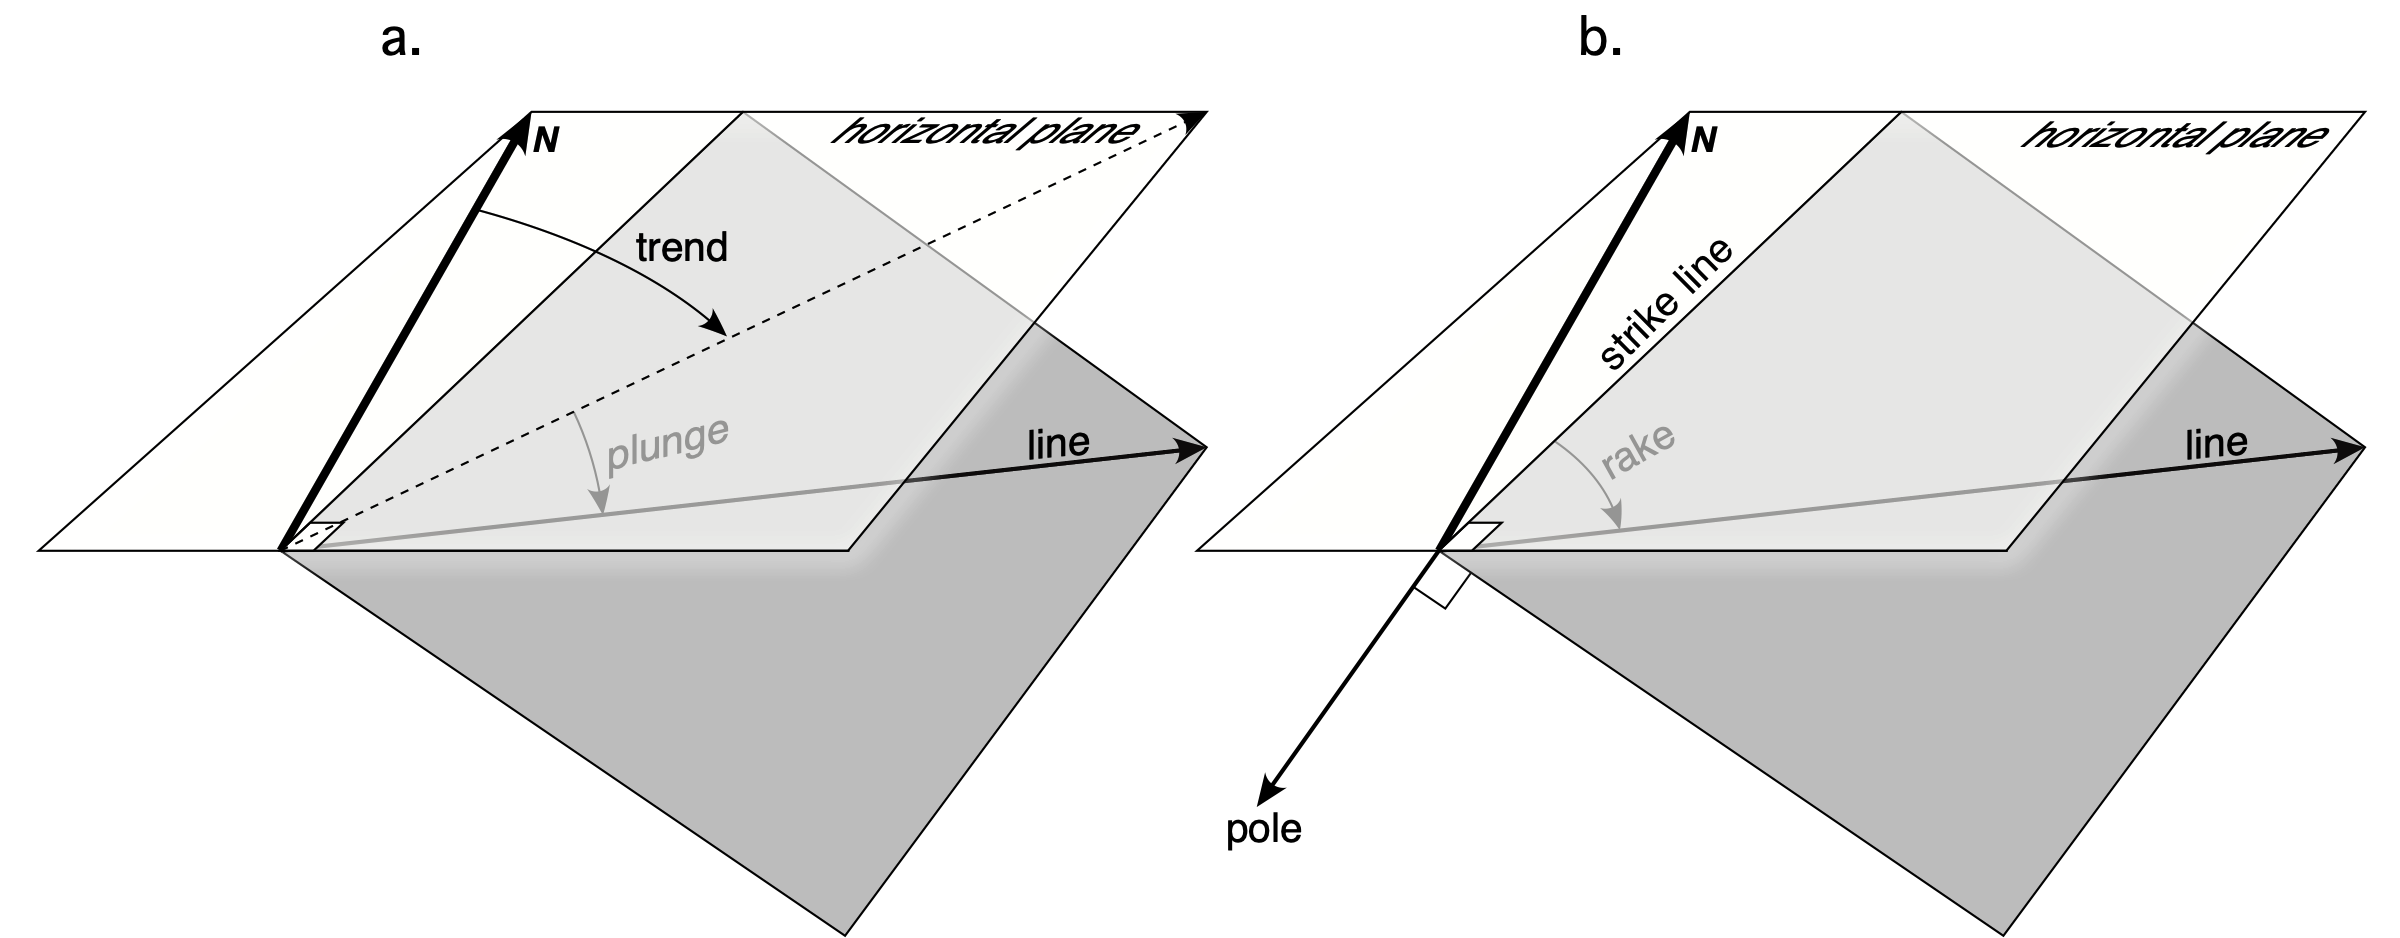
\includegraphics[width=13cm]{Figures/ch3f2.png}
    \caption{\textbf{a.} Trend and plunge of a line, \textbf{b}. Rake of a line and pole to a plane. Modified from Allmendinger et al. (2012).}
\end{figure}

% SUBSECTION: THE POLE TO THE PLANE
\subsection{The pole to the plane}

Any plane can be uniquely represented by its downward normal. This line is known as the pole to the plane (Fig. 3.2b). If we use the RHR format, the orientation of the pole is given by:

\begin{equation}
    \begin{split}
        trend\,of\,pole = strike\,of\,plane -90\degree \\
        plunge\,of\,pole = 90\degree - dip\,of\,plane
    \end{split}
\end{equation}

The pole facilitates analyzing planes graphically and by computation. Our first function \href{https://github.com/nfcd/compGeo/blob/master/source/functions/Pole.py}{\textit{Pole}} computes the pole to a plane (\textit{k} = 1) or the plane from its pole (\textit{k} = 0). It is followed by the helper function \href{https://github.com/nfcd/compGeo/blob/master/source/functions/ZeroTwoPi.py}{\textit{ZeroTwoPi}} which makes sure azimuths are always between 0 and 360\degree. Notice that angles (\textit{trd} and \textit{plg}) should be entered in radians, and the plane must follow the RHR format.

\begin{center}
\begin{lstlisting}[language=Python, frame=single]
import math
from ZeroTwoPi import ZeroTwoPi as ZeroTwoPi

def Pole(trd,plg,k):
    '''
    Pole returns the pole to a plane or the plane from a pole  

    If k = 0, Pole returns the strike (trd1) and dip (plg1)
    of a plane, given the trend (trd) and plunge (plg) 
    of its pole.

    If k = 1, Pole returns the trend (trd1) and plunge (plg1) 
    of a pole, given the strike (trd) and dip (plg) 
    of its plane.

    NOTE: Input/Output angles are in radians. 
    Input/Output strike and dip follow the RHR format

    Pole uses function ZeroTwoPi
    '''
    # Some constants
    east = math.pi/2

    # Eq. 3.2
    # Calculate plane given its pole
    if k == 0:
        if plg >= 0:
            plg1 = east - plg
            trd1 = ZeroTwoPi(trd + east)
        else: # Unusual case of pole pointing upwards
            plg1 = east + plg
            trd1 = ZeroTwoPi(trd - east) 
    # Else calculate pole given its plane
    elif k == 1:
    	plg1 = east - plg;
    	trd1 = ZeroTwoPi (trd - east)
        
    return trd1, plg1
\end{lstlisting}
\end{center}

\begin{center}
\begin{lstlisting}[language=Python, frame=single]
import math

def ZeroTwoPi(a):
    '''
    This function makes sure input azimuth (a)
    is within 0  to 2*pi (b)
    
    NOTE: Azimuths a and b are input/output in radians
    
    Python function translated from the Matlab function 
    ZeroTwoPi in Allmendinger et al. (2012)
    '''
    b=a
    twopi = 2*math.pi
    if b < 0:
        b += twopi
    elif b >= twopi:
        b -= twopi
        
    return b
\end{lstlisting}    
\end{center}

% SUBSECTION: INSTRUMENTS USED IN THE FIELD
\subsection{Instruments used in the field}

Traditionally, geologists use a geological compass/clinometer to measure the orientation of planes and lines in the field. Figure 3.3 shows four of the most common compasses used in geology: the Silva compass (Fig. 3.3a), the Brunton compass (Fig. 3.3b), the Krantz compass (Fig. 3.3c, a less expensive variant of the Freiberg compass), and the Brunton Geo compass (Fig. 3.3d). All these compasses have a magnetic needle that points  to the magnetic north (N or white end of the needle), a horizontal level, and a clinometer (an instrument to measure vertical angles). The Silva compass has an azimuth scale that can be rotated to follow the magnetic needle, while in the other three compasses the azimuth scale is fixed. This is why east-west (E-W) are in the right place in the Silva compass, while they are flipped in the other three compasses (Fig. 3.3a-d).

\begin{figure}[ht]
    \centering
    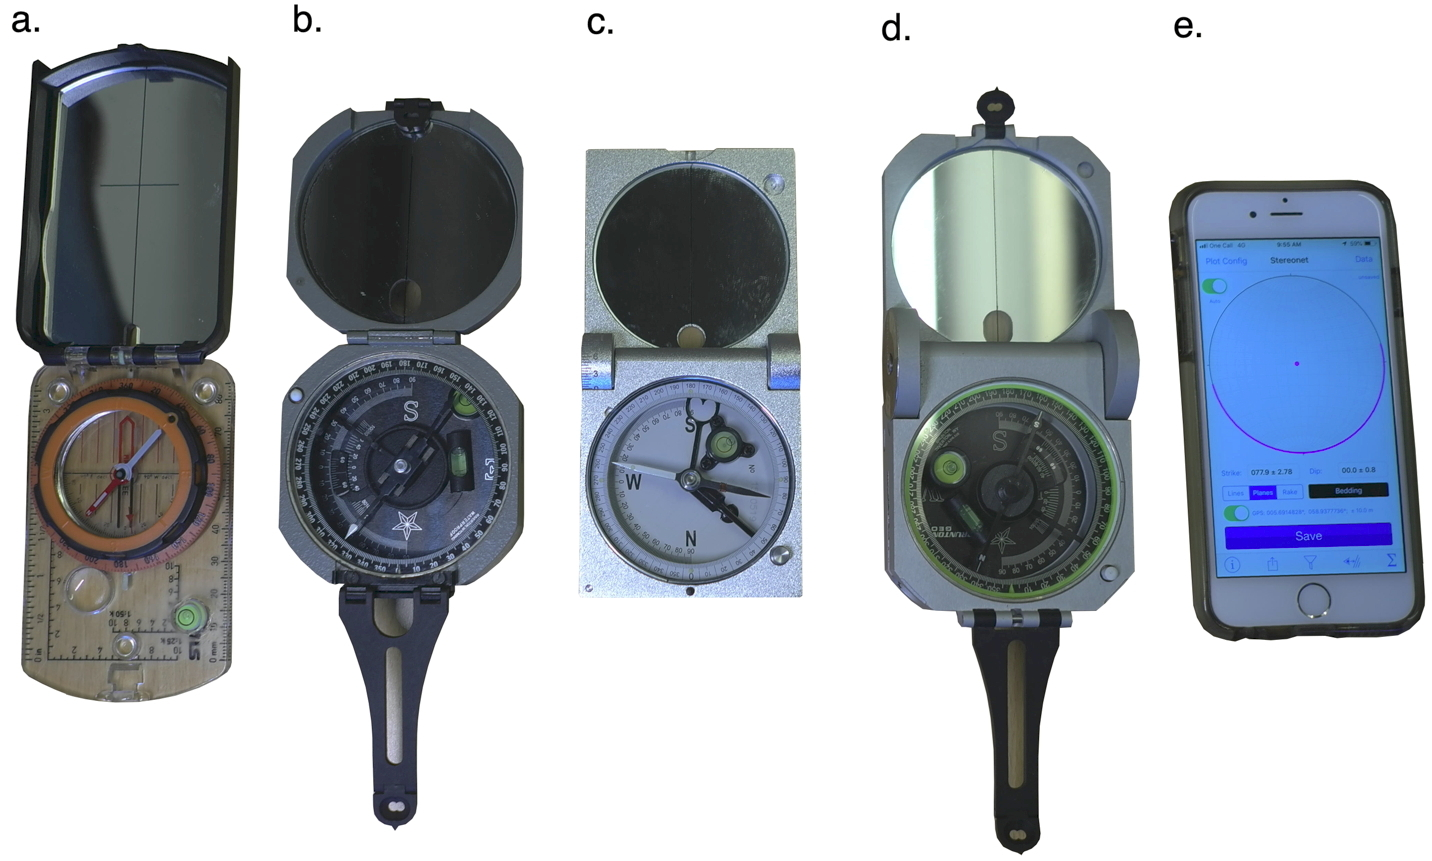
\includegraphics[width=13cm]{Figures/ch3f3.png}
    \caption{\textbf{a.} Silva, \textbf{b.} Brunton, \textbf{c.} Krantz, \textbf{d.} Brunton Geo, and \textbf{e.} Smartphone with Stereonet Mobile.}
\end{figure}

The Silva and Brunton compasses are designed to measure strike and dip through two measurements, while the Krantz compass measures dip direction and dip at once. The Brunton Geo compass can work either as a Brunton or Krantz compass, and it has higher precision than the other three compasses (it is also the most expensive). The use of these compasses is well explained in field geology books such as Compton (1985) and Coe (2010). For illustration, Figure 3.4 shows how strike and dip are measured with the Brunton compass (the same principles apply to the Silva compass). Notice that in this measurement, it is crucial to determine when the compass is horizontal (Fig. 3.4a). We will see that this can be a source of error (section 3.2.5).

\begin{figure}[ht]
    \centering
    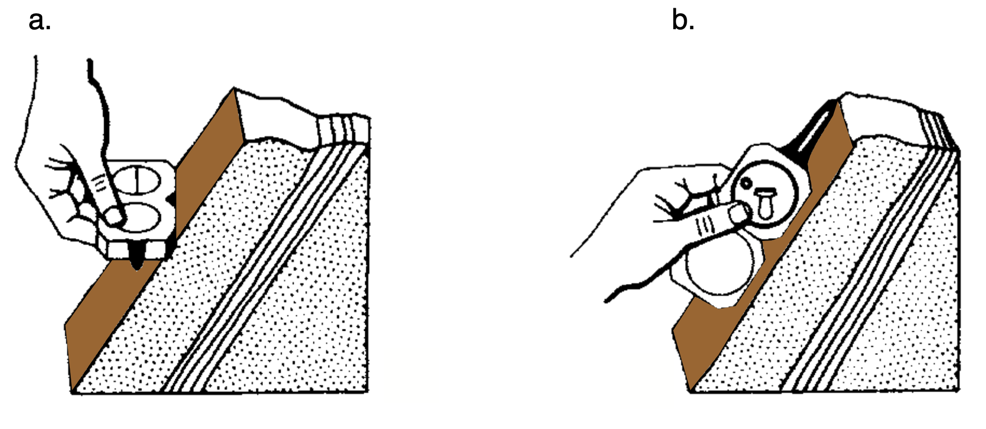
\includegraphics[width=12cm]{Figures/ch3f4.png}
    \caption{Measuring the \textbf{a.} strike and \textbf{b.} dip of a plane. Modified from Compton (1985).}
\end{figure}

These days, digital devices in the form of smartphone programs or apps (Fig. 3.3e) are slowly replacing the analog compasses. Smartphones contain instruments such as accelerometers, gyroscopes, and magnetometers, which enable apps such as \href{http://www.geo.cornell.edu/geology/faculty/RWA/programs/stereonet-mobile.html}{Stereonet Mobile} (Richard Allmendinger) or \href{https://www.petex.com/products/move-suite/digital-field-mapping/}{Fieldmove Clino} (Petroleum Experts) to determine the exact orientation of the device in space. Measuring a plane or a line just requires placing the phone on the plane or along the line. Thus, one can capture a large number of measurements quickly. However, smartphones are very sensitive to nearby magnetic fields and one can easily get spurious results (Novakova and Plavlis, 2017). Smartphones also have access to accurate geographic location (GPS, cell and wireless networks) as well as satellite imagery and raster data such as elevation. They can greatly facilitate mapping in the field.

% SUBSECTION: UNCERTAINTIES
\subsection{Uncertainties in orientations} \label{uncertainties}

Geological planes and lines are irregular and therefore it is difficult to take exact measurements of them. Every plane or line measurement has an uncertainty (an error). There are different ways to try to reduce this error, either by placing a smooth planar object (e.g. a field notebook) on the plane or along the line, or by sighting the plane or line from the distance (Compton, 1985). Figure 3.5 illustrates the error associated to the strike and dip measurement of a plane. If the compass is not exactly horizontal then a direction other than the strike will be measured. The departure of the compass from the horizontal or operator error ($\varepsilon_o$) will give a strike error ($\varepsilon_s$).

\begin{figure}[ht]
    \centering
    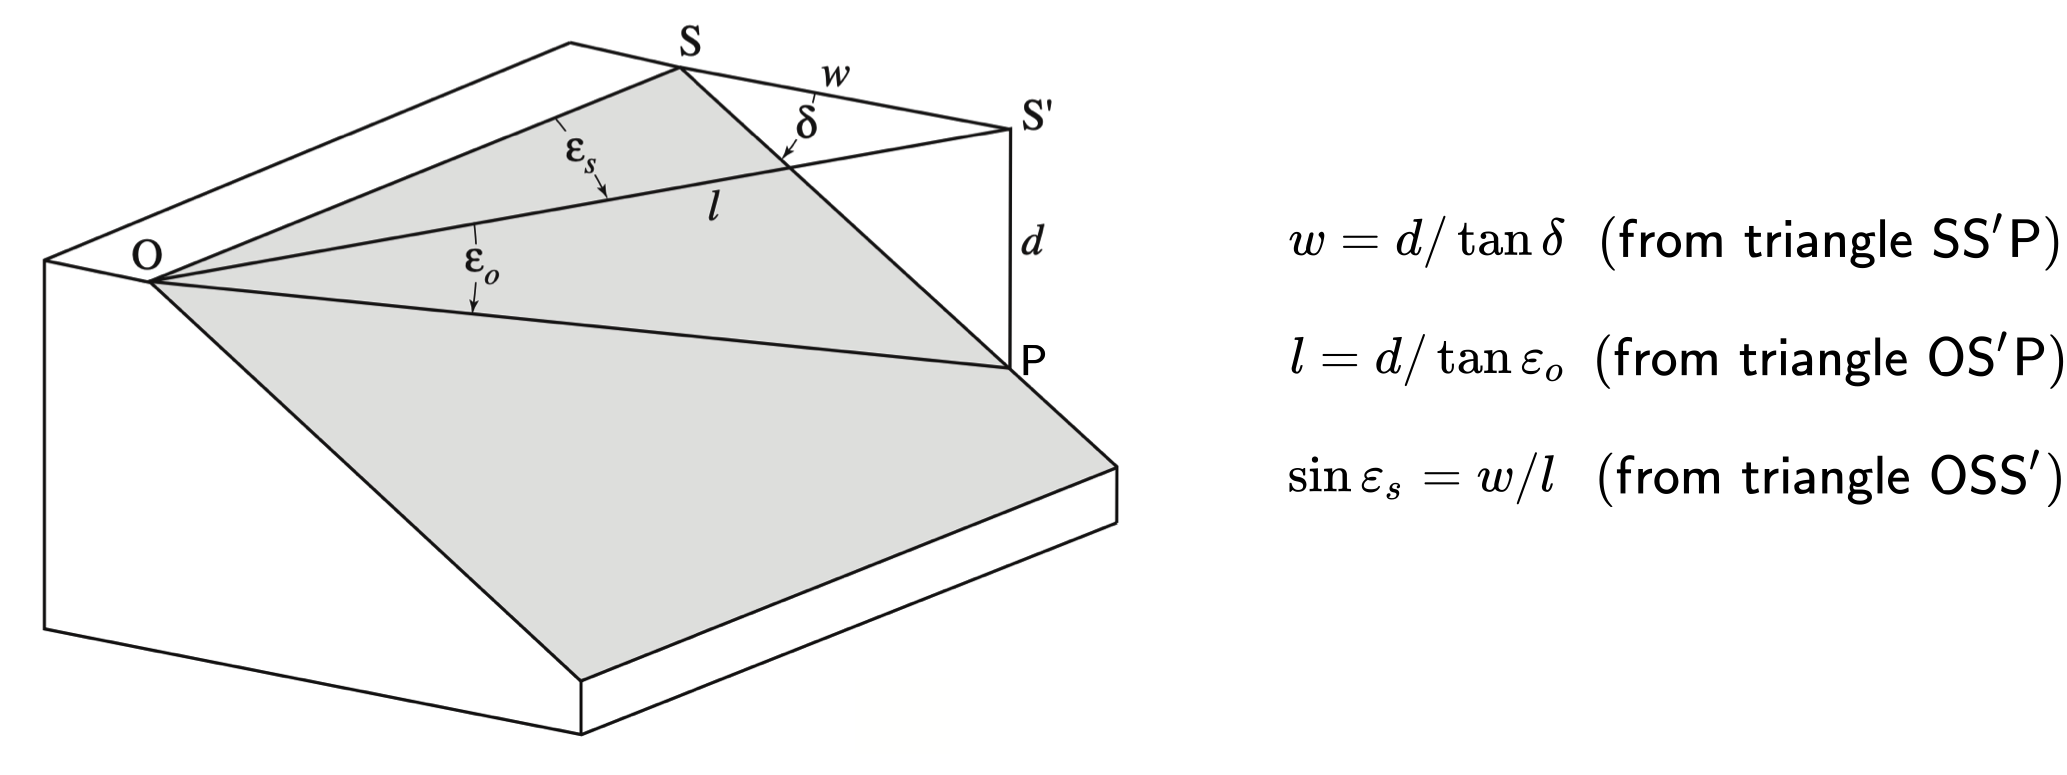
\includegraphics[width=13cm]{Figures/ch3f5.png}
    \caption{Geometrical relations for estimating the strike error $\varepsilon_s$ from the operator error (or departure of the compass from the horizontal) $\varepsilon_o$.  Modified from Ragan (2009).}
\end{figure}

From the three right-triangles and their corresponding equations in Figure 3.5, and by substituting the first two equations for \textit{w} and \textit{l} into the third equation for $\varepsilon_s$, one gets the following relation (Woodcock, 1976):

\begin{equation}
    \sin\varepsilon_s = \frac{\tan\varepsilon_o}{\tan\delta}
\end{equation}

where $\delta$ is the dip angle of the plane. This equation is plotted in Figure 3.6 for dip angles $\delta$ of 0 to 40\degree and operator errors $\varepsilon_o$ of 1 to 5\degree. It is clear that the strike error $\varepsilon_s$ increases with decreasing dip. For a gentle 5\degree dipping plane, an operator error $\varepsilon_o$ of 2\degree (a compass just 2\degree off the horizontal) results in a strike error $\varepsilon_s$ of about 24\degree! Thus, one should always be suspicious about the accuracy of strike and dip measurements, particularly if they are from gently dipping planes.

\begin{figure}[ht]
    \centering
    {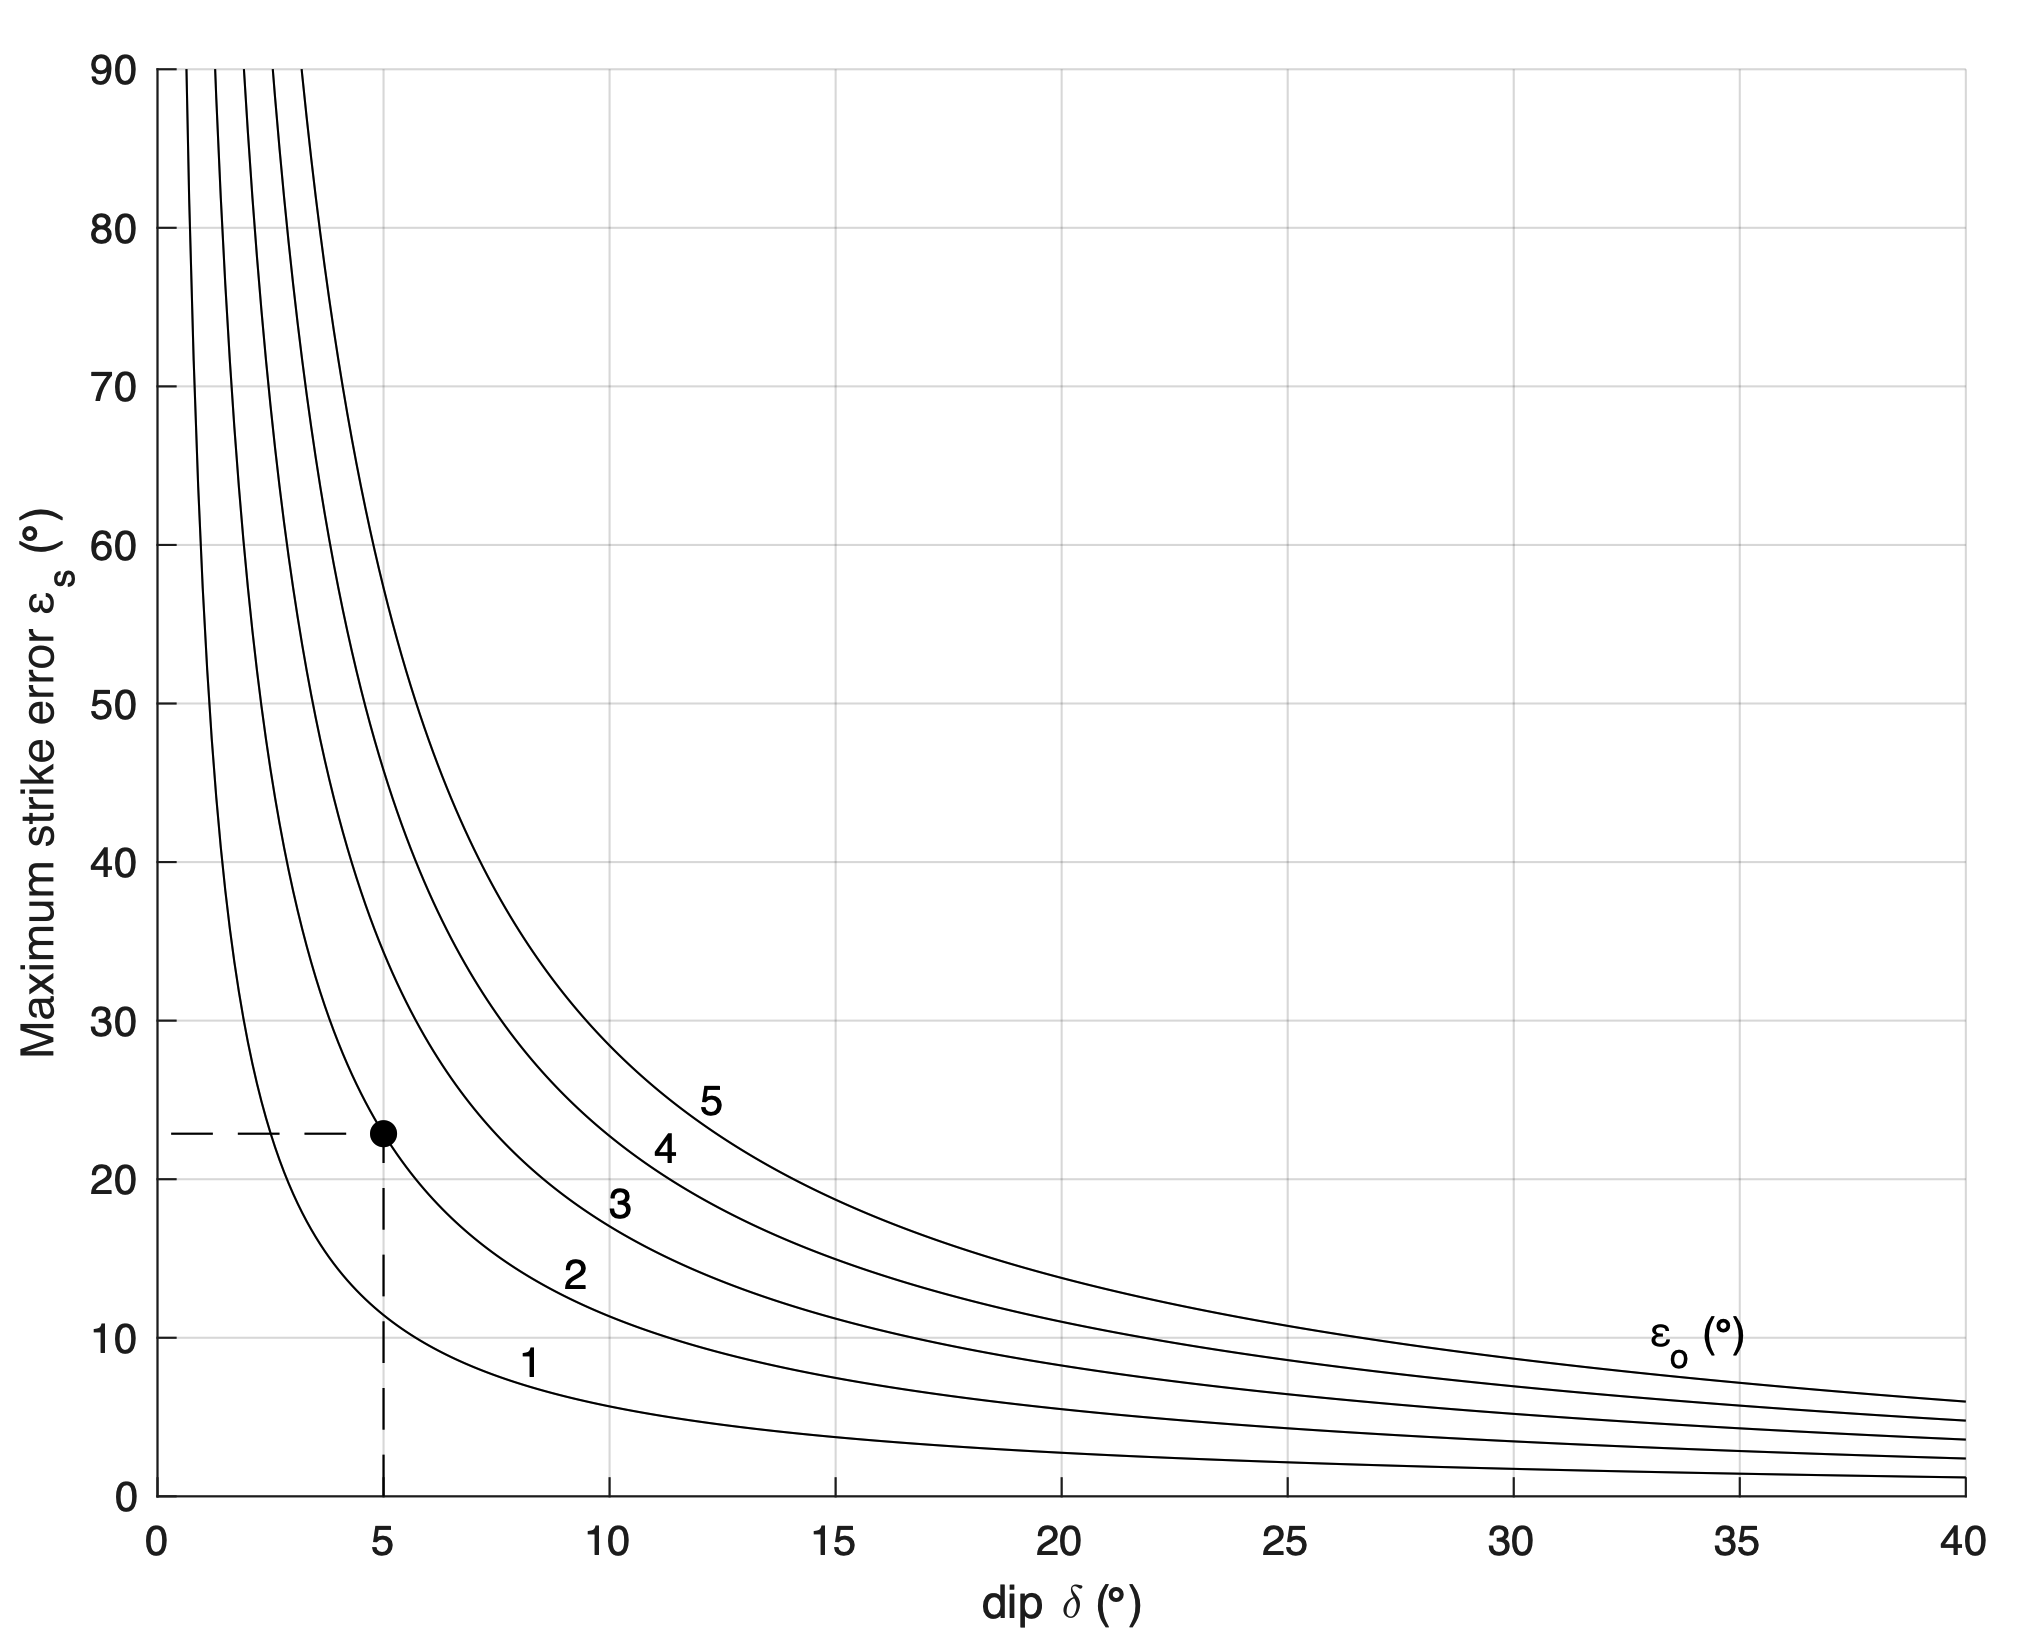
\includegraphics[width=13cm]{Figures/ch3f6.png}}
    \caption{Strike error $\varepsilon_s$ as a function of dip $\delta$ for values of operator error $\varepsilon_o$  of 1-5\degree. The \href{https://github.com/nfcd/compGeo/blob/master/source/notebooks/ch3fig6.ipynb}{notebook} that produced this graph is available from the resource git repository.}
\end{figure}

For line measurements, the situation is not better. When measuring the orientation of a line, it is common practice to align the compass in the direction of the horizontal projection of the line, which, as anyone who has tried this in the field knows, it is quite difficult. There will be an operator error and the measured trend $\beta\text{$'$}$ will differ from the true trend $\beta$ (Fig. 3.7a). The trend error $\varepsilon_t$ ($|\beta\text{$'$}- \beta|$)in terms of the angle on the plane $\varepsilon_o$ which the measured line makes with the true line, is given by the following equations (Woodcock, 1976): 

\begin{figure}[ht]
    \centering
    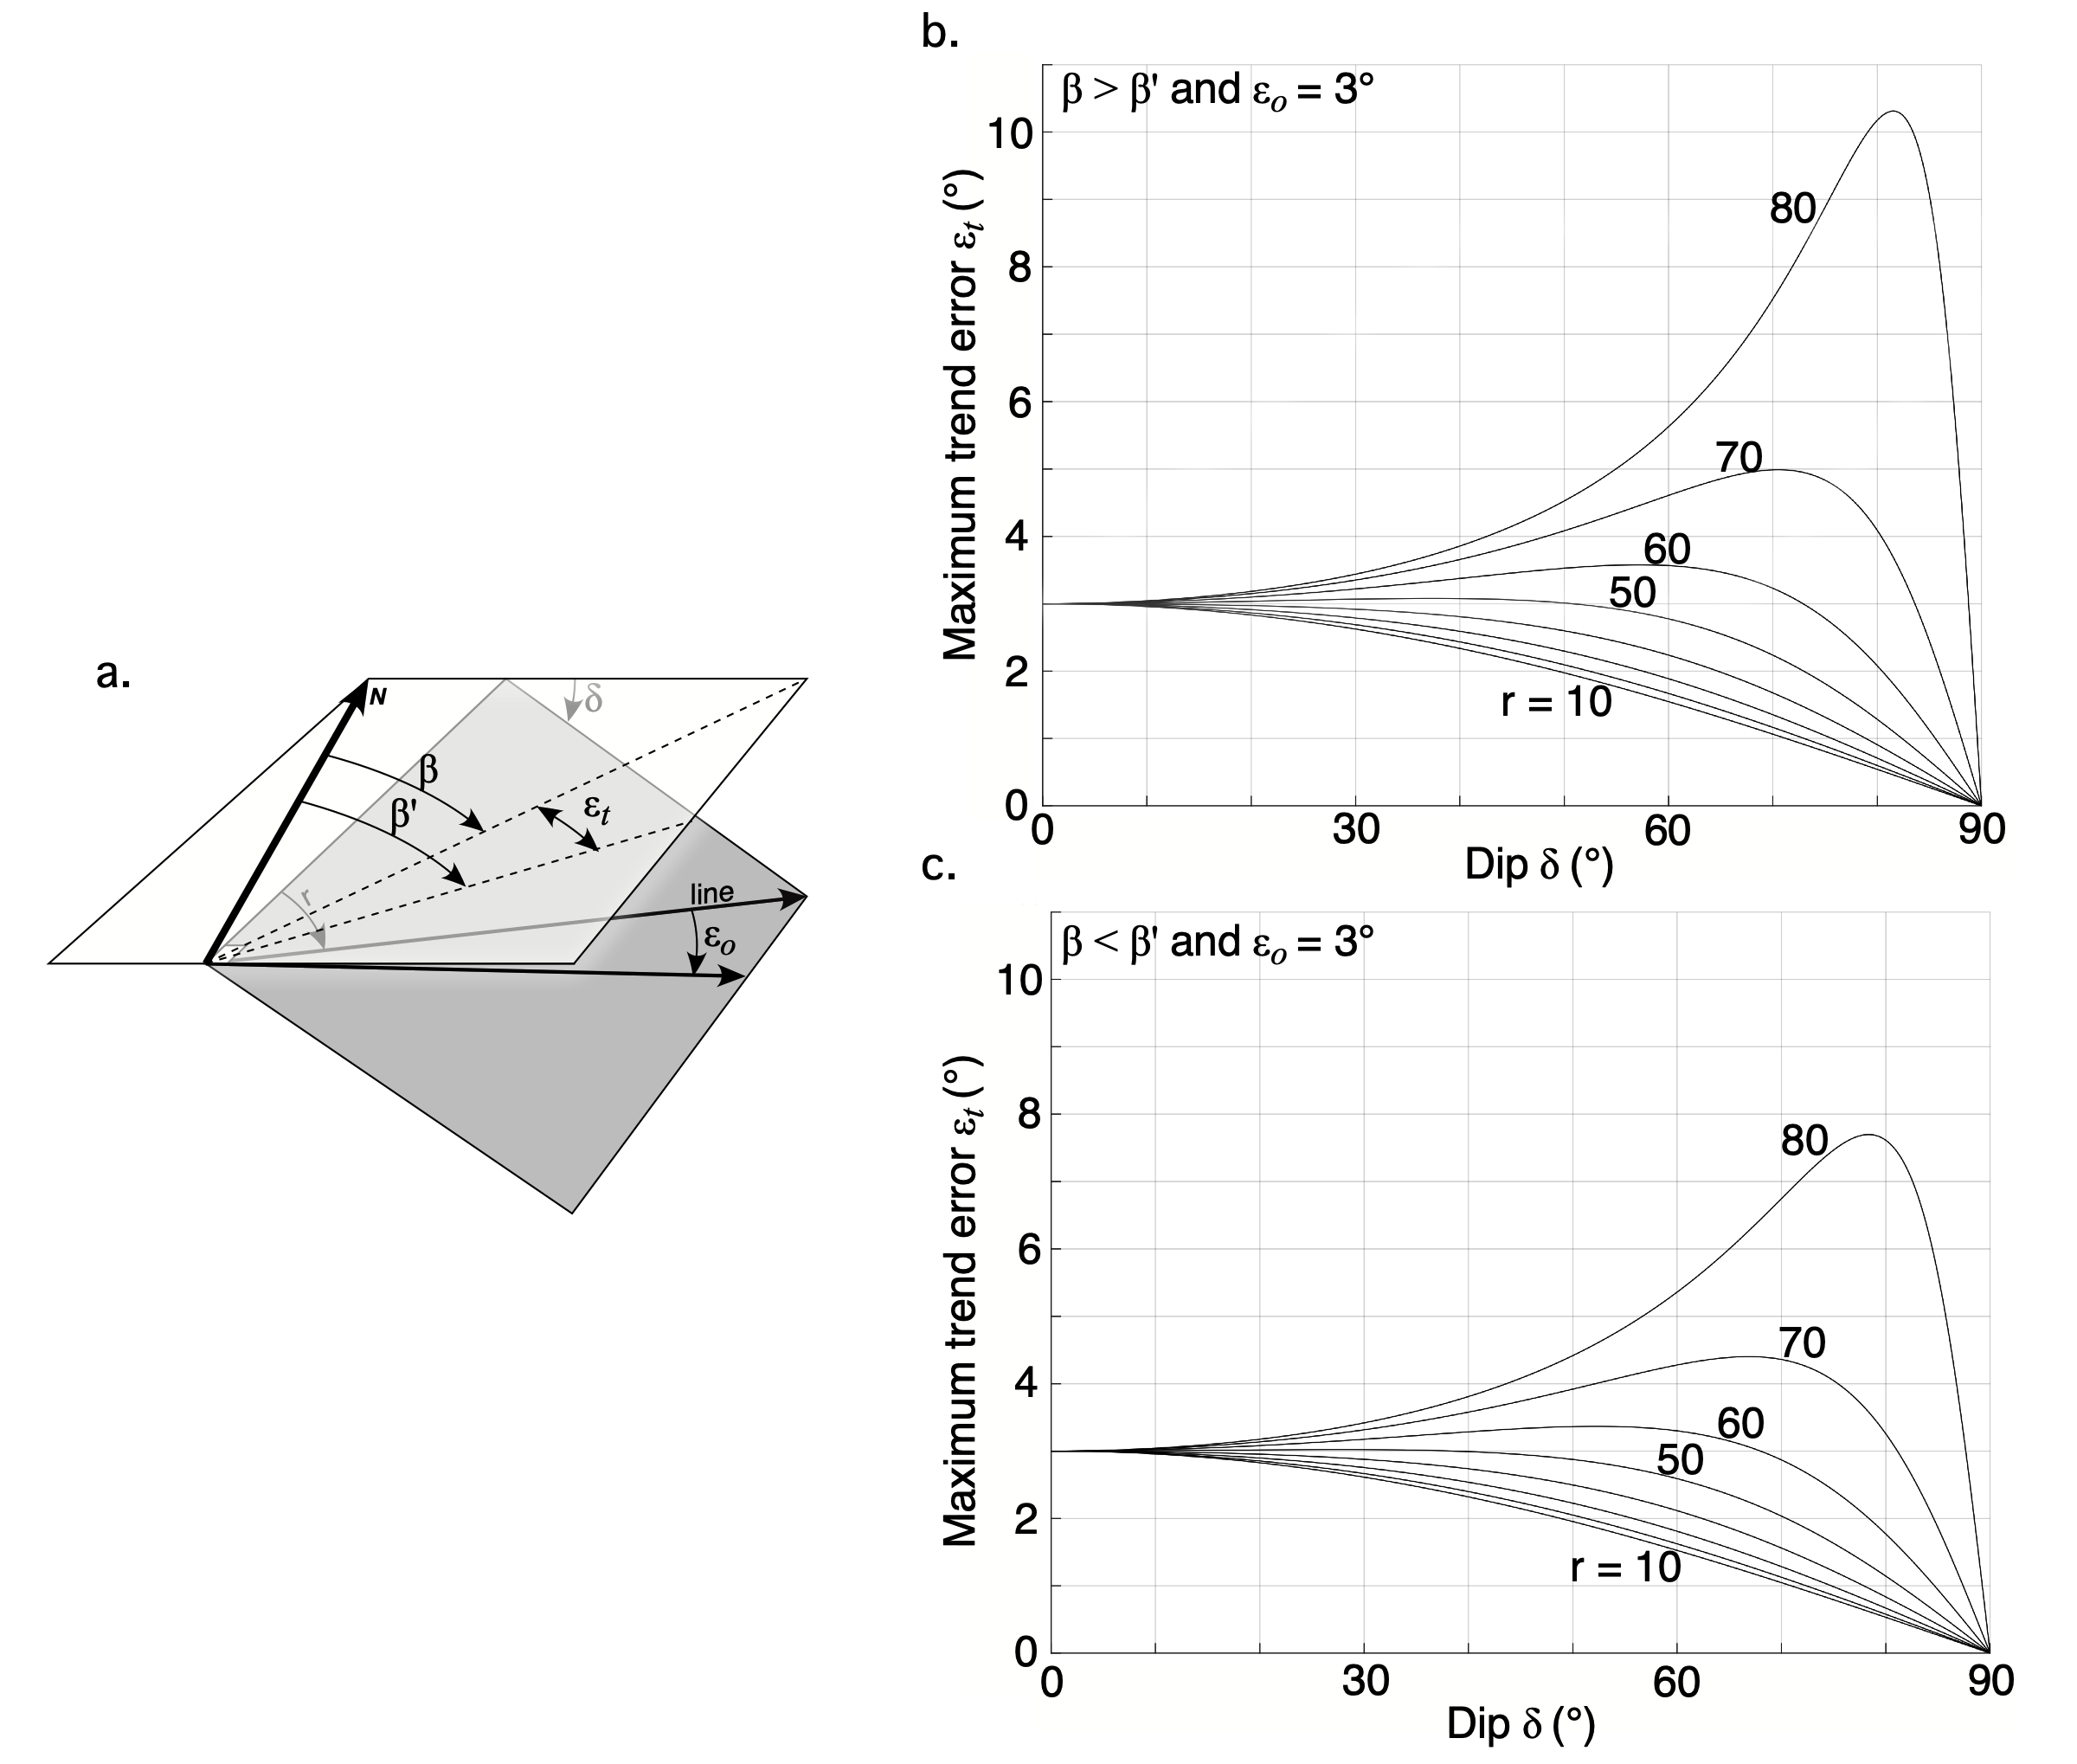
\includegraphics[width=13cm]{Figures/ch3f7.png}
    \caption{\textbf{a.} Geometrical relations for estimating the trend error $\varepsilon_t$ from the rake \textit{r} of the line, the dip $\delta$  of the plane, and the angle on the plane $\varepsilon_o$ between the measured and the true lines. Trend error as function of dip for \textbf{b.} a measured line on the down-dip side of the line, and \textbf{c.} a measured line on the up-dip side of the line. In b and c, $\varepsilon_o$ is 3\degree. The notebooks that produced graphs \href{https://github.com/nfcd/compGeo/blob/master/source/notebooks/ch3fig7b.ipynb}{b} and \href{https://github.com/nfcd/compGeo/blob/master/source/notebooks/ch3fig7c.ipynb}{c} are available from the resource git repository.}
\end{figure}

\begin{equation}
    \begin{split}
        \tan\varepsilon_t = \frac{[\tan(r+\varepsilon_o)-\tan(r)]\cos\delta}{1+[\tan(r+\varepsilon_o)\tan(r)]\cos^2\delta} \hspace{0.5cm} if \beta\text{$'$}>\beta\\ \\
        \tan\varepsilon_t = \frac{[\tan(r)-\tan(r-\varepsilon_o)]\cos\delta}{1+[\tan(r)\tan(r-\varepsilon_o)]\cos^2\delta} \hspace{0.5cm} if \beta\text{$'$}<\beta
    \end{split}
\end{equation}

where \textit{r} is the rake of the line, and $\delta$ is the dip of the plane (Fig. 3.7a). These equations are plotted in Figure 3.7b-c for an $\varepsilon_o$ of 3\degree. The trend error is greater for a measured line on the down-dip ($\beta\text{$'$} > \beta$) side of the line (Fig. 3.7b), than for a measured line on the up-dip ($\beta\text{$'$} < \beta$) side of the line (Fig. 3.7c). This means that repeated measurements will not be symmetrically distributed around the true trend $\beta$. Also for a given $\varepsilon_o$, the trend error $\varepsilon_t$ increases with the dip $\delta$ of the plane and the rake \textit{r} of the line, i.e. a combination of a steep plane and a large rake may result in a large trend error.

Equations 3.3 and 3.4 allow determining the uncertainties associated to the measurement of planes and lines. As we will see in section \ref{calcuncertainties}, these errors propagate in any computation making use of these orientations.

% SECTION: DISPLAYING GEOLOGIC FEATURES
\section{Displaying geologic features}

There are two fundamental ways geologists display geologic features: maps and stereonets. In maps, we are concerned about the location and orientation of the features, and the spatial relation of one feature to another. In stereonets, we are just concerned with the orientation of the features.

% SUBSECTION MAPS
\subsection{Maps}

All maps are a projection of surface or subsurface geologic features onto a horizontal plane. In section \ref{projections}, we looked at the different methods used to project data from the approximately spherical Earth to a flat surface, and the distortions associated to these methods. Geologic features (bedding, faults, the ground surface) are rarely flat, and therefore to display the spatial variation of their elevation (or depth) on maps, we use contours. A contour line is a line joining the points in the map area of equal value for a specific parameter. On a topographic map, for example, contour lines join points of equal elevation on the ground surface. Contour lines should not cross (unless very unusual circumstances) or disappear in the middle of the map (unless the contoured feature is intersected by another). If the difference in value between adjacent contours or contour interval is held constant throughout the map, the gradient (rate of change) of the parameter in a given direction is proportional to the spacing of the contour lines: high gradient is represented by closely spaced contours, and low gradient by widely spaced contours. This is expressed by the following relation:

\begin{equation}
    gradient = \arctan\frac{parameter\,change\,between\,contours}{map\,distance\,between\,contours} \tag{3.5a}
\end{equation}

For a topographic map, this relation becomes:

\begin{equation}
    slope\,angle = \arctan\frac{elevation\,change\,between\,contours}{map\,distance\,between\,contours} \tag{3.5b}
\end{equation}

which is why when choosing the walking path to a high ground area, you should look for the widely spaced contours (unless you are a climber or a goat).

Geologic features are rarely isolated, and they usually have different orientations, so we should expect them to intersect. The intersection of two non-parallel planes (e.g. bedding contacts) is a straight line. In chapter 4, we will see how to determine this type of intersection using vector operations. If one of the surfaces is not planar but is irregular, the intersection is a curved line which is more difficult to determine. One of the most fundamental mapping problem geology students are early confronted with is the intersection of a planar feature (e.g. bedding or a fault) with the irregular land surface. This is elegantly summarized by the \textit{Rule of V’s} (Fig. 3.8).

\begin{figure}[ht]
    \centering
    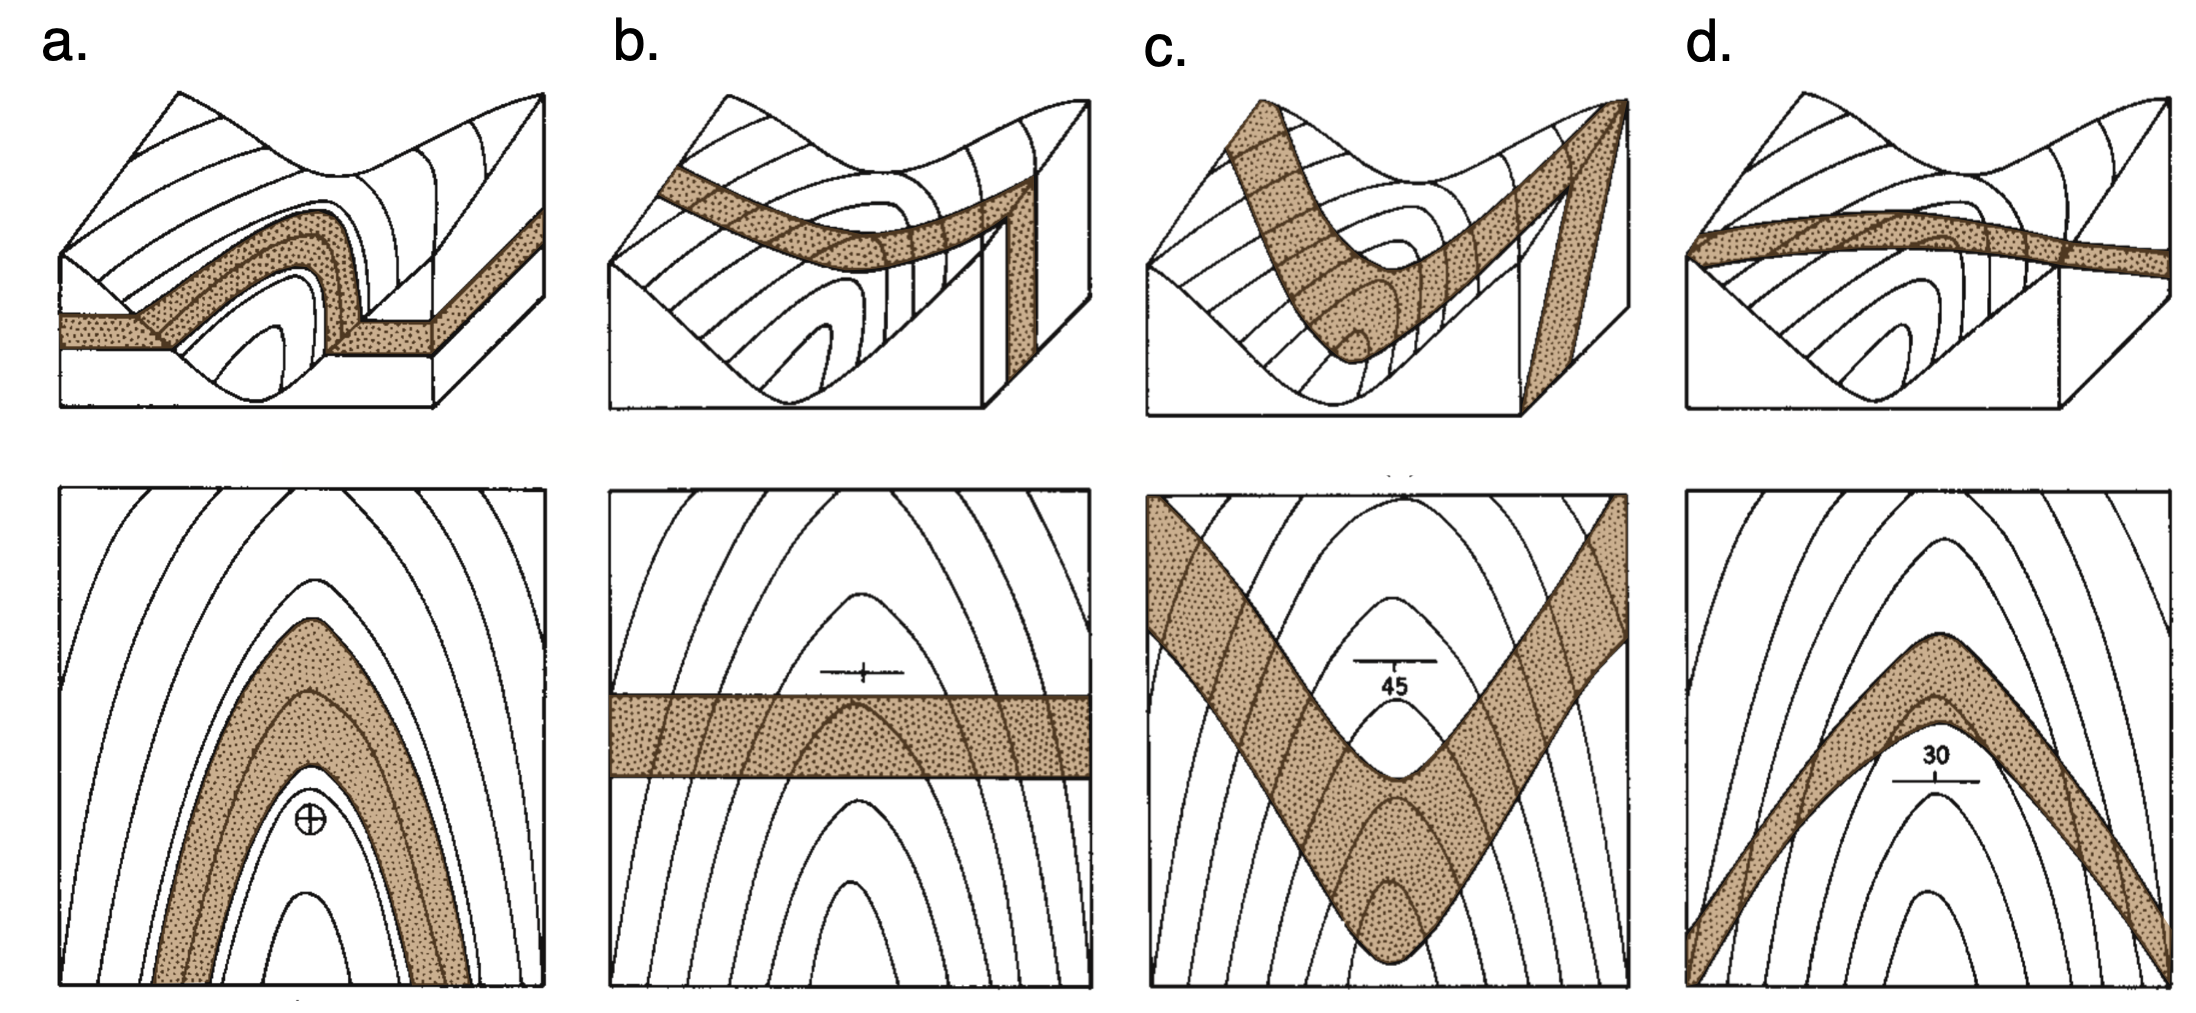
\includegraphics[width=13cm]{Figures/ch3f8.png}
    \caption{Outcrop pattern across a valley of \textbf{a.} Horizontal bed, \textbf{b.} Vertical bed, \textbf{c.} Bed dipping downstream, and \textbf{d.} Bed dipping upstream. Modified from Ragan (2009).}
\end{figure}

The Rule of V’s says that when a planar contact crosses a valley, its outcrop pattern will V or curve in the direction that the contact is dipping, but only if the contact if steeper than the slope of the valley, which is normally the case (Fig. 3.8c-d). There are two exceptions: 1. If the contact is horizontal, its outcrop pattern will follow the topographic contours, which makes sense since the contours are the intersection of horizontal planes of different elevation with the ground (Fig. 3.8a), and 2. If the contact is vertical, its outcrop pattern across the valley is a straight line. Vertical planes “ignore” topography.

Determining the outcrop trace of a planar contact on irregular topography is not straightforward. Graphically, this problem involves making elevation contours on the planar contact. These are called structure contours. Then one should look at the locations where the structure contours of the contact have the same elevation than the topographic contours of the land surface. On these locations, the contact outcrops. Finally, one should join these locations with a line, to make the outcrop trace of the contact. Figure 3.9 illustrates this procedure for a plane dipping north and intersecting irregular topography. Notice how in the stream valleys, the outcrop trace of the plane curves to the north, clearly following the Rule of V’s.

\begin{figure}[ht]
    \centering
    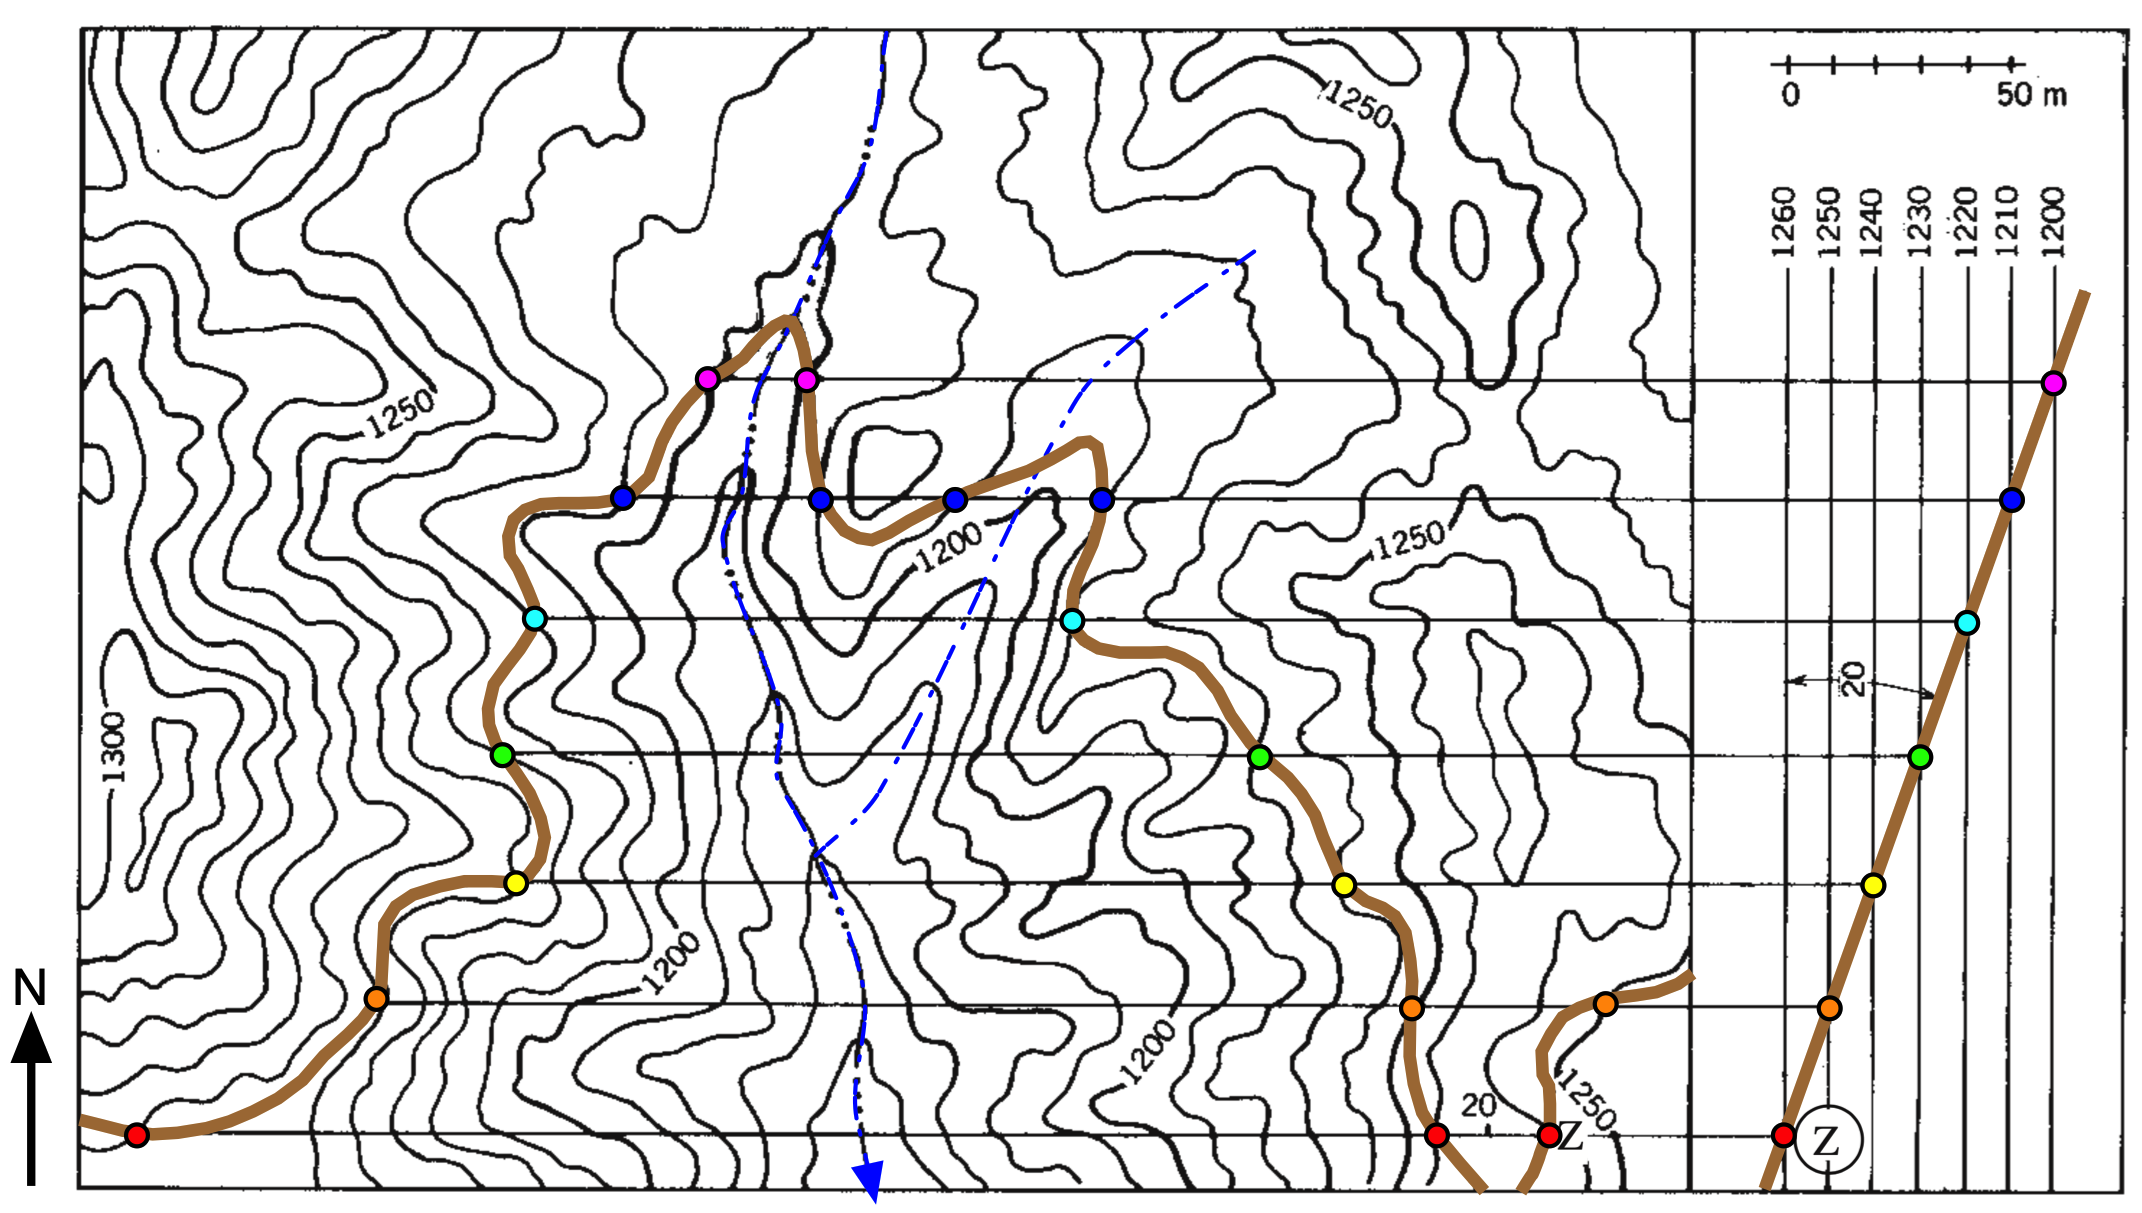
\includegraphics[width=13cm]{Figures/ch3f9.png}
    \caption{Outcrop trace of a plane dipping 20\degree N. The left figure is the map, and the right figure is a N-S cross section. Color points are the locations where the plane's structure contours have the same elevation than the topographic contours. The line joining these points is the outcrop trace of the plane. Modified from Ragan (2009).}
    \label{fig:outrace}
\end{figure}

This graphical approach requires a great deal of patience and drawing skills. Later in section \ref{outcrop}, we sill see that if we have the plane’s orientation and one outcrop location, it is possible to project the plane throughout the terrain using computation, provided we have a digital elevation model (DEM) of the terrain. This saves a lot of time and it’s a great way to quality control mapping, test different hypotheses, and take better decisions in the field.

% SUBSECTION: STEREONETS
\subsection{Stereonets}

Spherical projections can be used to represent the orientation of a plane or a line if the plane or line is positioned so that it passes through the center of the sphere. A plane will intersect the sphere along a great circle, and a line will pierce the sphere at a point (Fig. 3.10a). Obviously, it would be inconvenient to carry a sphere everywhere. Fortunately, it is possible to project the sphere onto a plane using, for example, an azimuthal projection (section \ref{projections}).

\begin{figure}[ht]
    \centering
    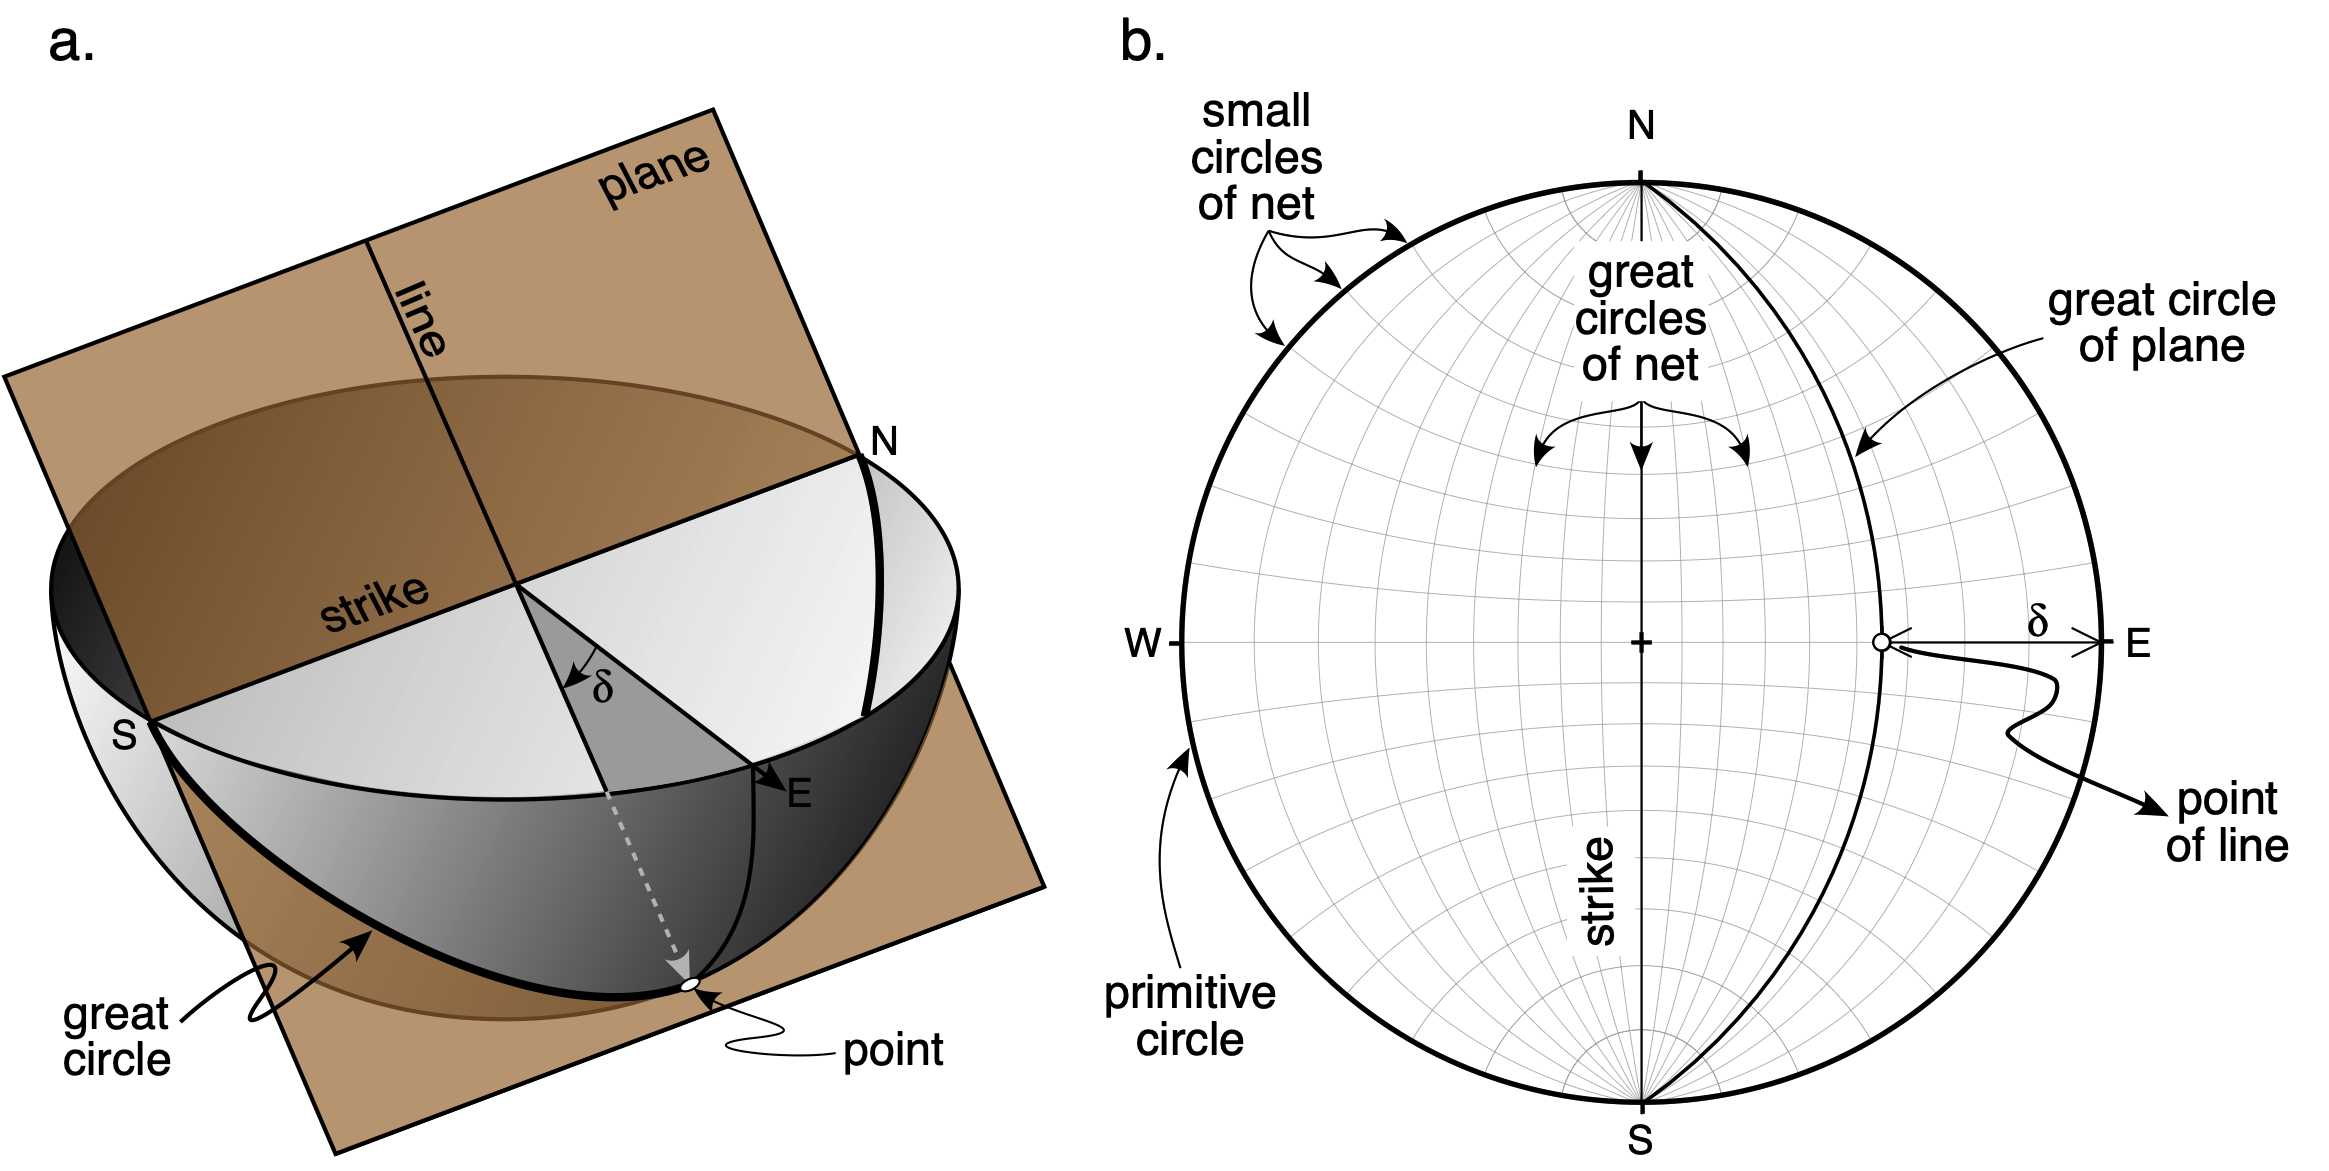
\includegraphics[width=13cm]{Figures/ch3f10.png}
    \caption{\textbf{a.} Plane and line intersecting the lower half of a sphere. The rake of the line is 90\degree and therefore its plunge is equal to the plane’s dip $\delta$. \textbf{b.} Lower hemisphere stereographic projection of plane and line. Modified from Allmendiger et al. (2012) and Allmendinger (2019).}
\end{figure}

A \textit{stereonet} or stereographic projection is a special kind of azimuthal projection, where the point source or viewpoint lies on the surface of the sphere, and the projection plane passes through the center of the sphere. In a stereonet, the viewpoint is at the top of the sphere or zenith, the view direction is downwards, the projection plane is the equatorial plane dividing the sphere into lower and upper hemispheres, and the lower hemisphere (bowl in Fig. 3.10a) is projected. In the stereonet, the rim of the bowl is called the primitive circle and it represents a horizontal plane (Fig. 3.10b). A net consisting of great circles representing N-S striking, 0-90\degree E and W dipping planes, and small circles representing cones of N-S horizontal axis and 0-90\degree apical radius opening to the S and N, helps drawing any plane or line (Fig. 3.10b). Several books explain how to do this and solve orientation problems (including rotations) using the stereonet (e.g. Marshak and Mitra, 1988).

For our purpose, it is more important to know how this projection actually works. Figure 3.11a illustrates this on a vertical section passing through the center of the sphere. Any line from the zenith (the top of the sphere) pinches the equatorial plane at one point, and this is the location where the point plots in the stereonet. This is defined by the following equation:

\begin{figure}[ht]
    \centering
    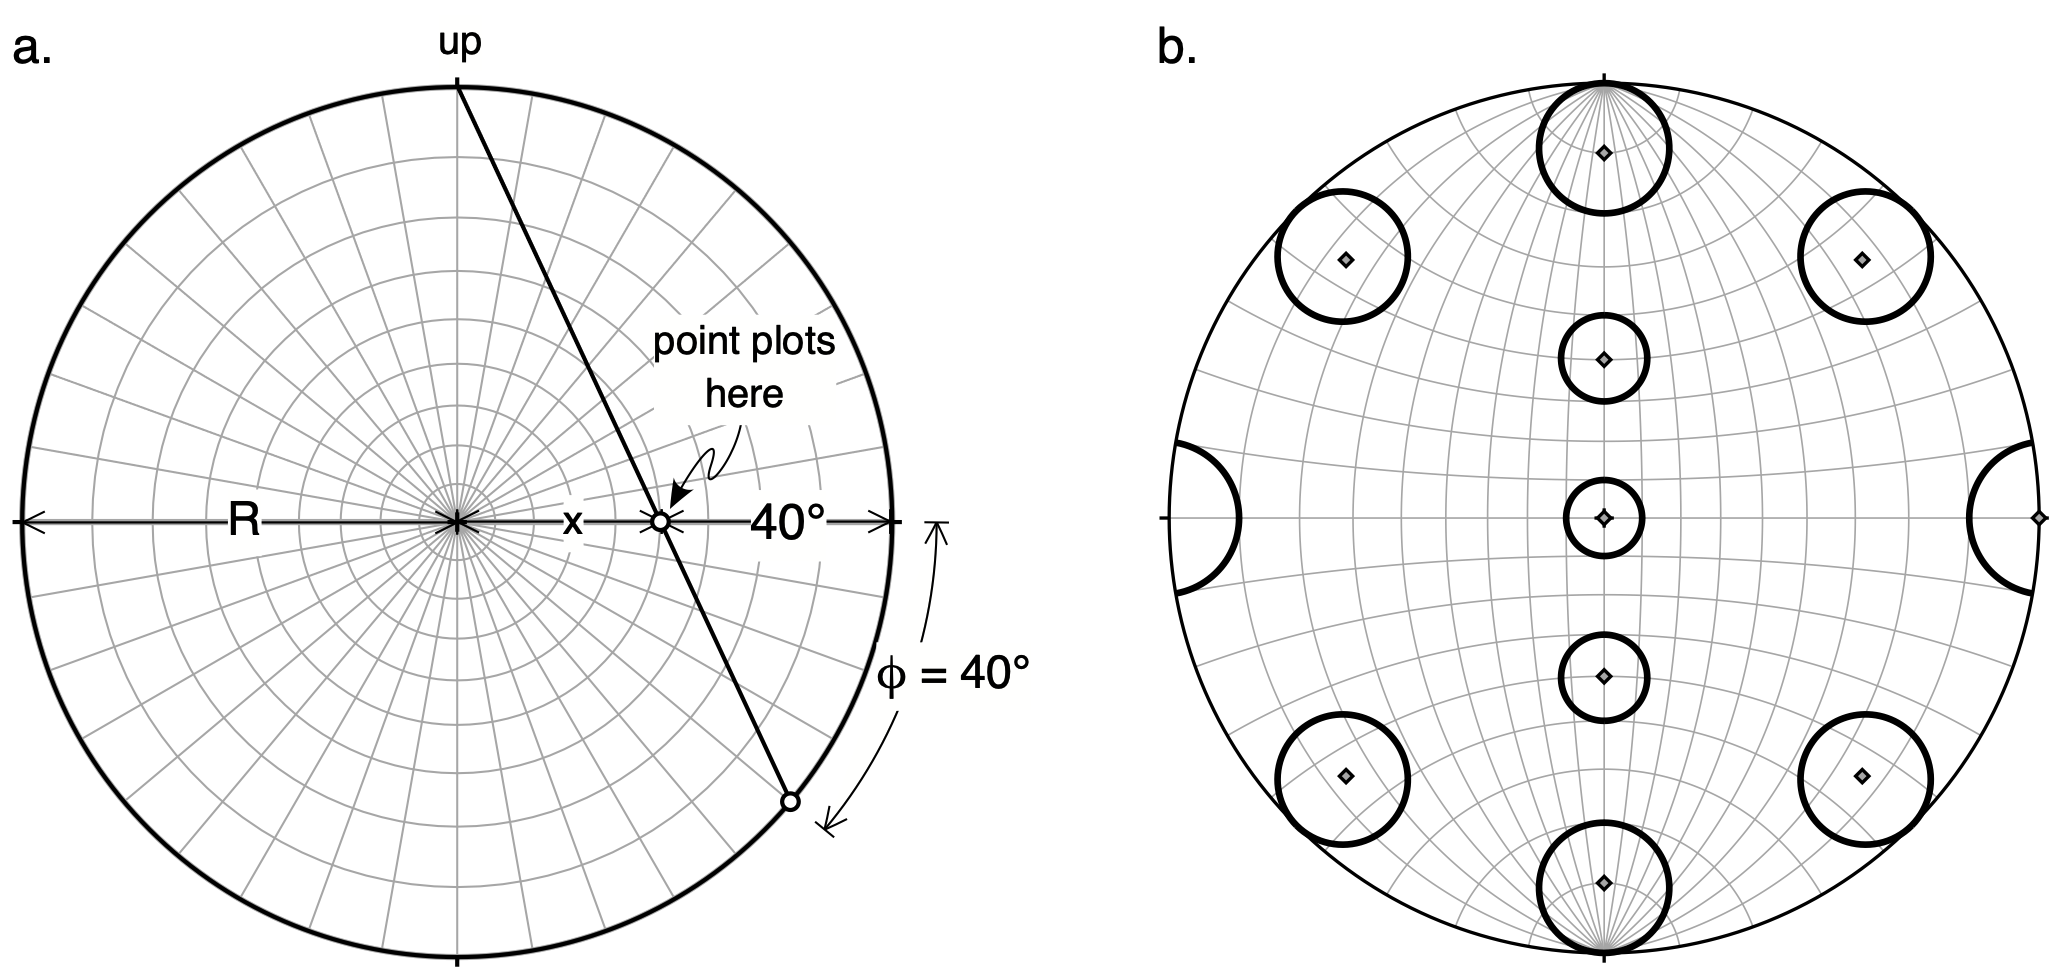
\includegraphics[width=13cm]{Figures/ch3f11.png}
    \caption{\textbf{a.} The equal angle stereonet illustrated on a vertical plane passing through the center of the sphere. \textbf{b.} Lower hemisphere equal angle projection of small circles of 10\degree radius but different axis orientations. Modified from Allmendinger et al. (2012).}
\end{figure}

\begin{equation}
    x = R\tan\left(45\degree-\frac{\phi}{2}\right) \tag{3.6}
\end{equation}

where \textit{x} is the is the distance of the point from the center of the net, \textit{R} is the radius of the net, and $\phi$ is the plunge of the line. This method preserves angles perfectly and thus, on the primitive circle, degrees are equally spaced, and a small circle will be a circle anywhere on the net (Fig. 3.11b). This is why this projection is called the equal angle or Wulff stereonet. However, the preservation of angles has a disadvantage: areas are distorted. Thus, for example, a 10\degree radius small circle will look smaller near the center of the net but larger near the edges (Fig. 3.11b). This poses a problem when trying to assess visually or graphically the density of points plotted on the net.

The equal area or Schmidt net (Fig. 3.12) overcomes this problem. Strictly speaking, this projection is not a stereographic projection because the projection plane is at the bottom of the sphere. The point of intersection of the line and the surface of the lower hemisphere, is projected to the horizontal plane at the lowest point of the sphere, along a circular arc centered at the bottom of the sphere. The \textit{x} distance of the point is then scaled by a factor of $\sqrt{2}$ to fit the radius \textit{R} of the net (Fig. 3.12a). This is expressed by the following equation:

\begin{figure}[ht]
    \centering
    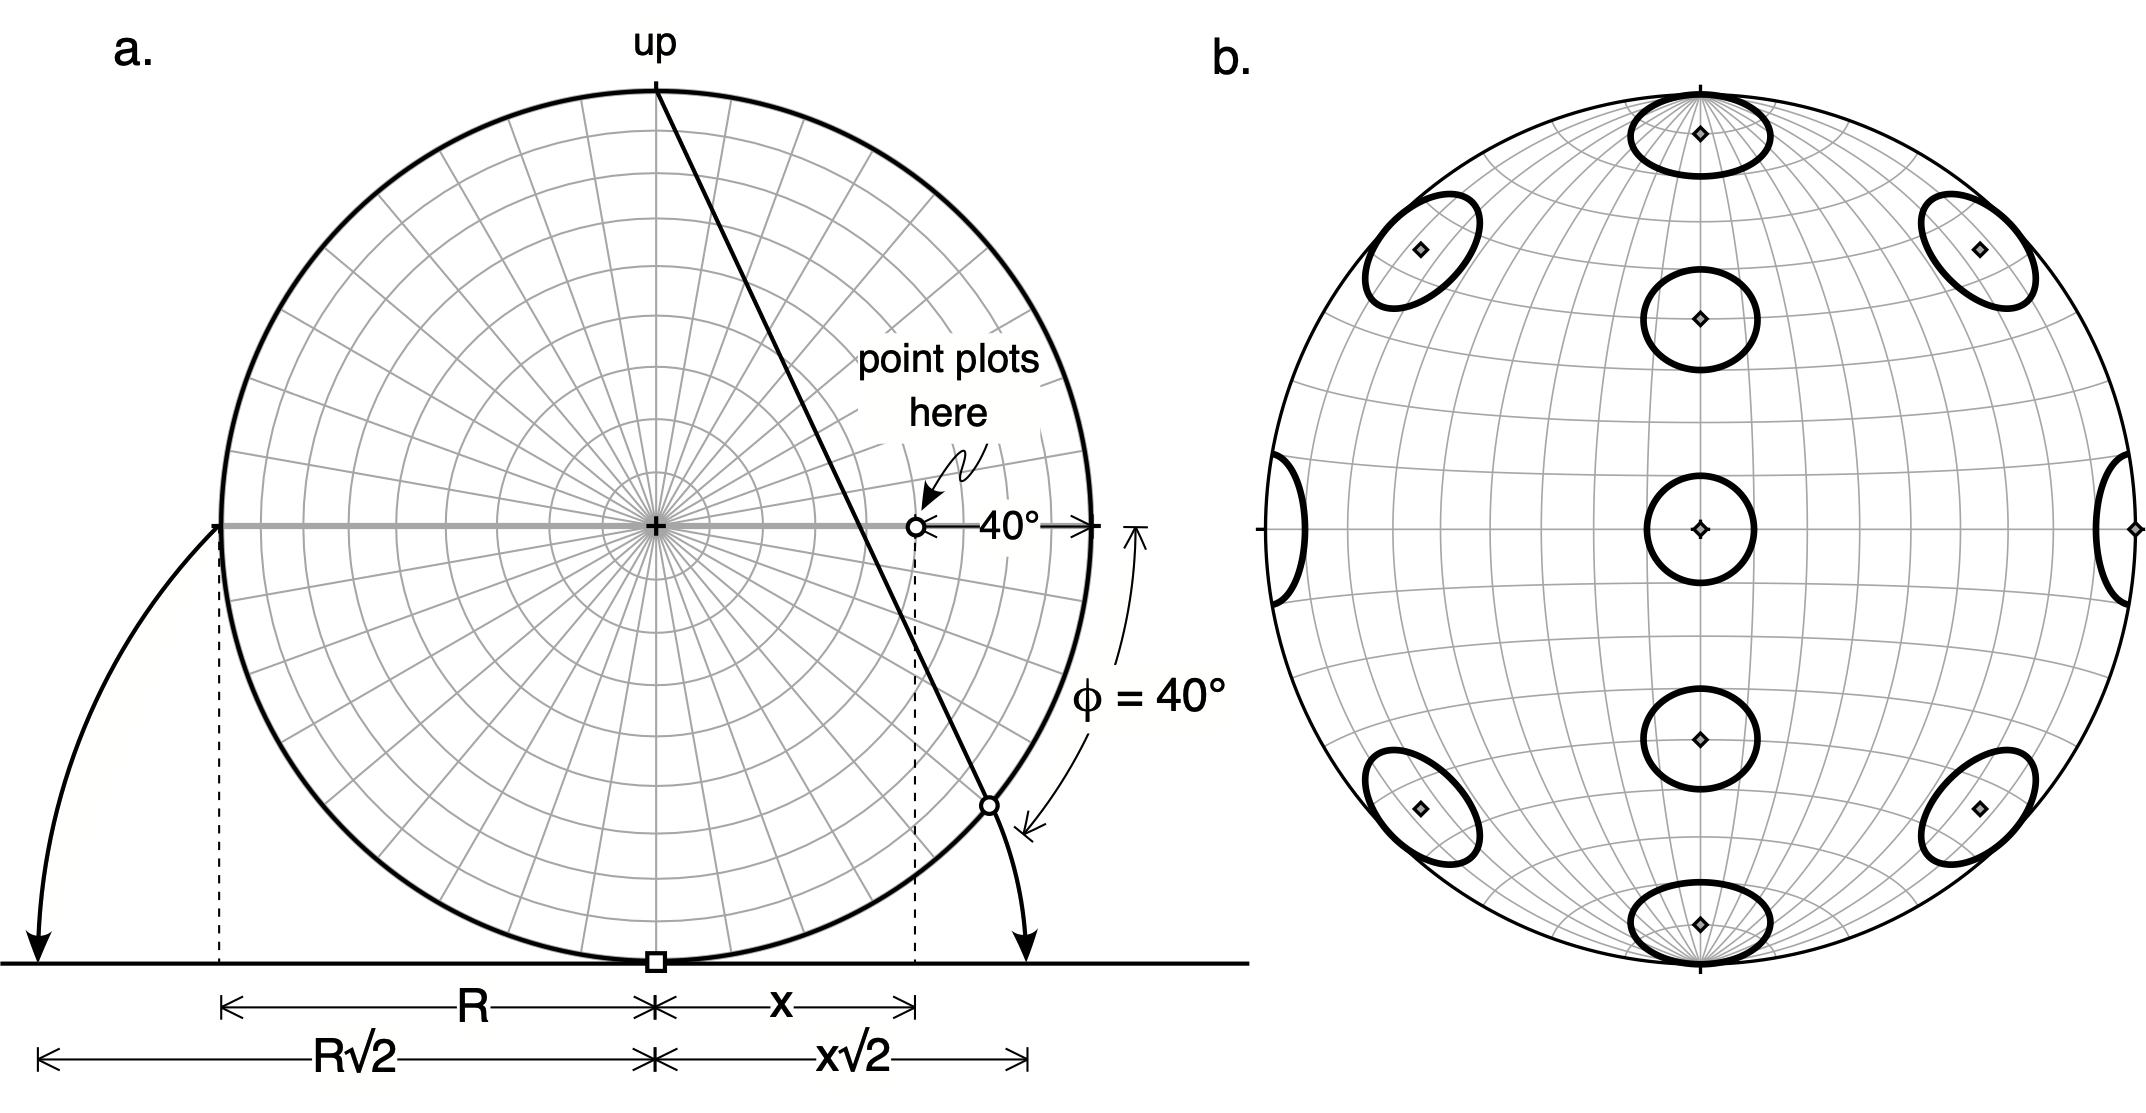
\includegraphics[width=13cm]{Figures/ch3f12.png}
    \caption{ \textbf{a.} The equal area stereonet illustrated on a vertical plane passing through the center of the sphere. \textbf{b.} Lower hemisphere equal area projection of small circles of 10\degree radius but different axis orientations. Modified from Allmendinger et al. (2012).}
\end{figure}

\begin{equation}
    x = R\sqrt{2}\sin\left(45\degree-\frac{\phi}{2}\right) \tag{3.7}
\end{equation}

The tradeoff is that angles are no longer preserved, and small circles are no longer true circles (Fig. 3.12b). The equal angle or Wulff net is used in problems where visualizing correctly angles on the net is important such as in crystallography and geography, while the equal area or Schmidt net is used in cases where analyzing the concentration of points on the net is important such as in structural analysis.

The function \href{https://github.com/nfcd/compGeo/blob/master/source/functions/StCoordLine.py}{\textit{StCoordLine}} computes the coordinates of a line in an equal angle or an equal area net (equations 3.7 and 3.8).  Notice that angles (\textit{trd} and \textit{plg}) should be entered in radians.

\begin{center}
\begin{lstlisting}[language=Python, frame=single]
import math
from ZeroTwoPi import ZeroTwoPi as ZeroTwoPi

def StCoordLine(trd,plg,sttype):
    '''
    StCoordLine computes the coordinates of a line 
    in an equal angle or equal area stereonet of unit radius
    
    trd  	= trend of line
    plg  	= plunge of line
    sttype 	= Stereonet type: 0 = equal angle, 1 = equal area
    xp and yp = Coordinates of the line in the stereonet

    NOTE: trend and plunge should be entered in radians

    StCoordLine uses function ZeroTwoPi
    
    Python function translated from the Matlab function 
    StCoordLine in Allmendinger et al. (2012)
    '''
    
    # Take care of negative plunges
    if plg < 0:
        trd = ZeroTwoPi(trd+math.pi)
        plg = -plg
        
    # Some constants
    piS4 = math.pi/4
    s2 = math.sqrt(2)
    plgS2 = plg/2
        
    # Equal angle stereonet, Eq. 3.6
    if sttype == 0:
        xp = math.tan(piS4 - plgS2)*math.sin(trd)
        yp = math.tan(piS4 - plgS2)*math.cos(trd)
    # Equal area stereonet, Eq. 3.7
    elif sttype == 1:
        xp = s2*math.sin(piS4 - plgS2)*math.sin(trd)
        yp = s2*math.sin(piS4 - plgS2)*math.cos(trd)
    
    return xp, yp
\end{lstlisting}   
\end{center}

% SUBSECTION: PLOTTING LINES AND POLES IN THE STEREONETS
\subsection{Plotting lines and poles in a stereonet}
The notebook \href{https://github.com/nfcd/compGeo/blob/master/source/notebooks/ch3.ipynb}{ch3} illustrates the use of the \textit{StCoordLine} and \textit{Pole} functions to plot lines and poles to planes on an equal angle or an equal area stereonet. You will get the chance to practice more with these functions in section \ref{exercises3}.

\begin{center}
\begin{lstlisting}[language=Python, frame=single]
import numpy as np
import matplotlib.pyplot as plt
%matplotlib inline

import sys
import os
sys.path.append(os.path.abspath('../functions'))
from Pole import Pole as Pole
from StCoordLine import StCoordLine as StCoordLine

# Plot the following four lines (trend and plunge)
# on an equal angle or equal area stereonet
lines = np.array([[30, 30],[120, 45],[210, 65],[280, 15]])
pi = np.pi
linesr = lines * pi/180 # lines in radians

# Plot the primitive of the stereonet
r = 1; # unit radius
TH = np.arange(0,360,1)*pi/180
x = r * np.cos(TH)
y = r * np.sin(TH)
plt.plot(x,y,'k')
# Plot center of circle
plt.plot(0,0,'k+')
# Make axes equal and remove them
plt.axis('scaled')
plt.axis('off')

# Find the coordinates of the lines in the
# equal angle or equal area stereonet
nrow, ncol = lines.shape
eqAngle = np.zeros((nrow, ncol))
eqArea = np.zeros((nrow, ncol))

for i in range(nrow):
    # Equal angle coordinates
    eqAngle[i,0], eqAngle[i,1] = StCoordLine(linesr[i,0],linesr[i,1],0) 
    # Equal area coordinates
    eqArea[i,0], eqArea[i,1] = StCoordLine(linesr[i,0],linesr[i,1],1)
    
# Plot the lines
# Equal angle as black dots
plt.plot(eqAngle[:,0],eqAngle[:,1],'ko')
# Equal area as red dots
plt.plot(eqArea[:,0],eqArea[:,1],'ro')
\end{lstlisting}
\fbox{
    \parbox{\textwidth - 2 \fboxsep}{
    Output: \\
    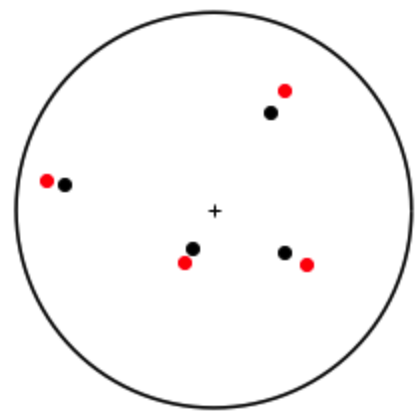
\includegraphics[width=4.75cm]{Figures/ch3f13.png}
}}
\end{center}

\begin{center}
\begin{lstlisting}[language=Python, frame=single]
# Plot the following four planes (strike and dip, RHR)
# as poles on an equal angle or equal area stereonet
planes = np.array([[0, 30], [90, 50], [180, 15], [270, 65]])
planesr = planes * pi/180 # planes in radians

# Plot the primitive of the stereonet
plt.plot(x,y,'k')
# Plot center of circle
plt.plot(0,0,'k+')
# Make axes equal and remove them
plt.axis('scaled')
plt.axis('off')

# Find the coordinates of the poles to the planes in the
# equal angle or equal area stereonet
for i in range(nrow):
    # Compute pole of plane
    trend, plunge = Pole(planesr[i,0],planesr[i,1],1)
    # Equal angle coordinates
    eqAngle[i,0], eqAngle[i,1] = StCoordLine(trend,plunge,0) 
    # Equal area coordinates
    eqArea[i,0], eqArea[i,1] = StCoordLine(trend,plunge,1)

# Plot the poles
# Equal angle as black asterisks
plt.plot(eqAngle[:,0],eqAngle[:,1],'k*')
# Equal area as red asterisks
plt.plot(eqArea[:,0],eqArea[:,1],'r*')
\end{lstlisting}
\fbox{
    \parbox{\textwidth - 2 \fboxsep}{
    Output: \\
    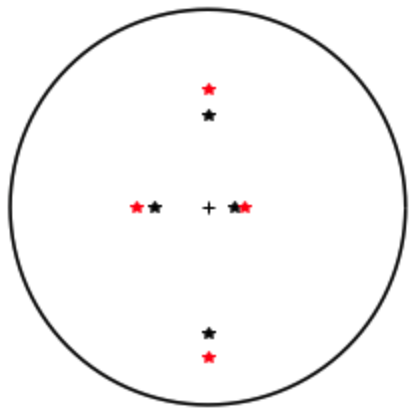
\includegraphics[width=4.75cm]{Figures/ch3f14.png}
}}
\end{center}

% SECTION: EXERCISES
\section{Exercises} \label{exercises3}

\begin{enumerate}
  \item Modify the notebook that makes Fig. 3.6 to extend the range of dip $\delta$ angles from 0 to 90\degree and the operator error $\varepsilon_o$ from 1 to 10\degree.
  
  \item Modify the notebooks that make Fig. 3.7 b and c for an $\varepsilon_o$ of 5\degree.
  
  \item You can draw a great circle on a stereonet by plotting closely spaced points along the great circle. These are lines on the plane. The following arrays contain the trend and plunge of lines on a plane of orientation 030/40 (strike and dip, RHR format):
  
  trend = [30, 34, 38, 42, 46, 50, 54, 58, 63, 67, 72, 78, 83, 89, 95, 101, 107, 113, 120, 127, 133, 139, 145, 151, 157, 162, 168, 173, 177, 182, 186, 190, 194, 198, 202, 206, 210]
  
  plunge = [0, 3, 6, 10, 13, 16, 19, 22, 24, 27, 29, 32, 34, 36, 37, 38, 39, 40, 40, 40, 39, 38, 37, 36, 34, 32, 29, 27, 24, 22, 19, 16, 13, 10, 6, 3, 0]
  
  Plot these lines on an equal angle and an equal area stereonet. From the resulting great circle, can you guess how a plane of orientation 050/60 (RHR) would look like on the stereonet? 
  
  \item You can also draw a small circle on a stereonet by plotting closely spaced points along the small circle. These are lines on the conical surface. The following arrays contain the trend and plunge of lines on a small circle of axis 050/30 (trend and plunge) and radius 20\degree:
  
  trend = [50, 53, 57, 60, 63, 66, 68, 70, 72, 73, 73, 73, 72, 70, 68, 64, 60, 55, 50, 45, 40, 36, 32, 30, 28, 27, 27, 27, 28, 30, 32, 34 37, 40, 43, 47, 50]
  
  plunge = [10, 10, 11, 12, 14, 16, 19, 22, 25, 28, 31, 35, 38, 41, 44, 47, 48, 50, 50, 50, 48, 47, 44, 41, 38, 35, 31, 28, 25, 22, 19, 16 14, 12, 11, 10, 10]
  
  Plot these lines on an equal angle and an equal area stereonet. What are the differences between the small circle in the equal angle and equal area stereonets?
  
  \item The strike and dip arrays below contain the strike and dip (RHR format) of 50 bedding surfaces in a fold:
  
  strike = [8, 22, 19, 33, 27, 37, 41, 47, 55, 40, 32, 55, 65, 68, 89, 79, 102, 105, 108, 122, 132, 136, 145, 159, 156, 164, 176, 169, 179, 173, 167, 160, 145, 148, 141, 125, 108, 92, 75, 57, 50, 39, 22, 10, 1, 9, 15, 16, 114, 78]
  
  dip = [75, 79, 68, 72, 61, 46, 50, 67, 51, 66, 55, 42, 49, 58, 54, 45, 35, 49, 63, 45, 52, 66, 52, 59, 76, 64, 72, 83, 78, 88, 72, 81, 73, 62, 50, 63, 42, 48, 56, 62, 50, 65, 76, 87, 81, 68, 74, 83, 56, 37]
  
  Plot these planes as poles in an equal area stereonet. The resultant diagram is called a \textit{point-}, \textit{scatter-} or $\pi-$ diagram. You can approximate a great circle through the poles. What is the approximate orientation of this great circle? What does the pole to this great circle represent?
  
\end{enumerate}

% SECTION: REFERENCES
\addcontentsline{toc}{section}{References}
\section*{References}

Allmendinger, R.W., Cardozo, N. and Fisher, D.W. 2012. Structural Geology Algorithms: Vectors and Tensors. Cambridge University Press, 302 p.

Allmendinger, R.W. 2019. Modern Structural Practice: A structural geology laboratory manual for the 21st century. [\href{http://www.geo.cornell.edu/geology/faculty/RWA/structure-lab-manual}{Online}]. [Accessed January, 2020].

Coe, A. 2010. Geological Field Techniques. Wiley-Blackwell, 323 p.

Compton, R.R. 1985. Geology in the field. John Wiley \& Sons, 398 p.

Novakova, L. and Pavlis, T.L. 2017. Assessment of the precision of smart phones and tablets for measurement of planar orientations: A case study. Journal of Structural Geology 97, 93-103.

Marshak, S. and Mitra, G. 1988. Basic Methods of Structural Geology. Prentice Hall, 446 p.

Ragan, D.M. 2009. Structural Geology: An Introduction to Geometrical Techniques. Cambridge University Press, 632 p.

Woodcock, N.H. 1976. The accuracy of structural field measurements. Journal of Geology 84, 350-355.

% CHAPTER 4: COORDINATE SYSTEMS AND VECTORS
\chapter{Coordinate systems and vectors}

Strike and dip, and trend and plunge, are a convenient way to represent the orientation of planes and lines. However, it is difficult to handle these angles using computation. In this chapter, we will see how to convert linear features (lines and poles to planes) from spherical (trend and plunge) to Cartesian (direction cosines) coordinates, thus representing these features as vectors. This facilitates the analysis of planes and lines using linear algebra and computation, and it will allow us to solve a range of interesting problems using vector operations.

% SECTION: Coordinate systems
\section{Coordinate systems}

Any point or location in space can be represented by the coordinates of the point with respect to the three orthogonal axes of a Cartesian coordinate system. We will call the three axes of this coordinate system $\mathbf{X_1}$, $\mathbf{X_2}$ and $\mathbf{X_3}$ (Fig. 4.1). In addition, we will follow a right-handed naming convention: If you hold your right hand so that your thumb points in the positive direction of the first axis $\mathbf{X_1}$, your other fingers should curl from the positive direction of the second axis $\mathbf{X_2}$ toward the positive direction of the third axis $\mathbf{X_3}$ (Fig. 4.1). Such a coordinate system is called a right-handed coordinate system.

In geosciences, we use mainly two types of right-handed coordinate systems: An east (\textbf{E}), north (\textbf{N}), up (\textbf{U}) coordinate system (Fig. 4.1a), and a north (\textbf{N}), east (\textbf{E}), down (\textbf{D}) coordinate system (Fig. 4.1b). The \textbf{ENU} coordinate system is used in GIS and Geophysics when dealing with elevations (e.g. topography), while the \textbf{NED} coordinate system is used in Structural Geology where, by convention, angles measured downwards from the horizontal (e.g. plunge of a downward pointing line) are considered positive. In this chapter, we will use the \textbf{NED} coordinate system, but when dealing with topography and elevations, we will use the \textbf{ENU} coordinate system.

\begin{figure}[ht]
    \centering
    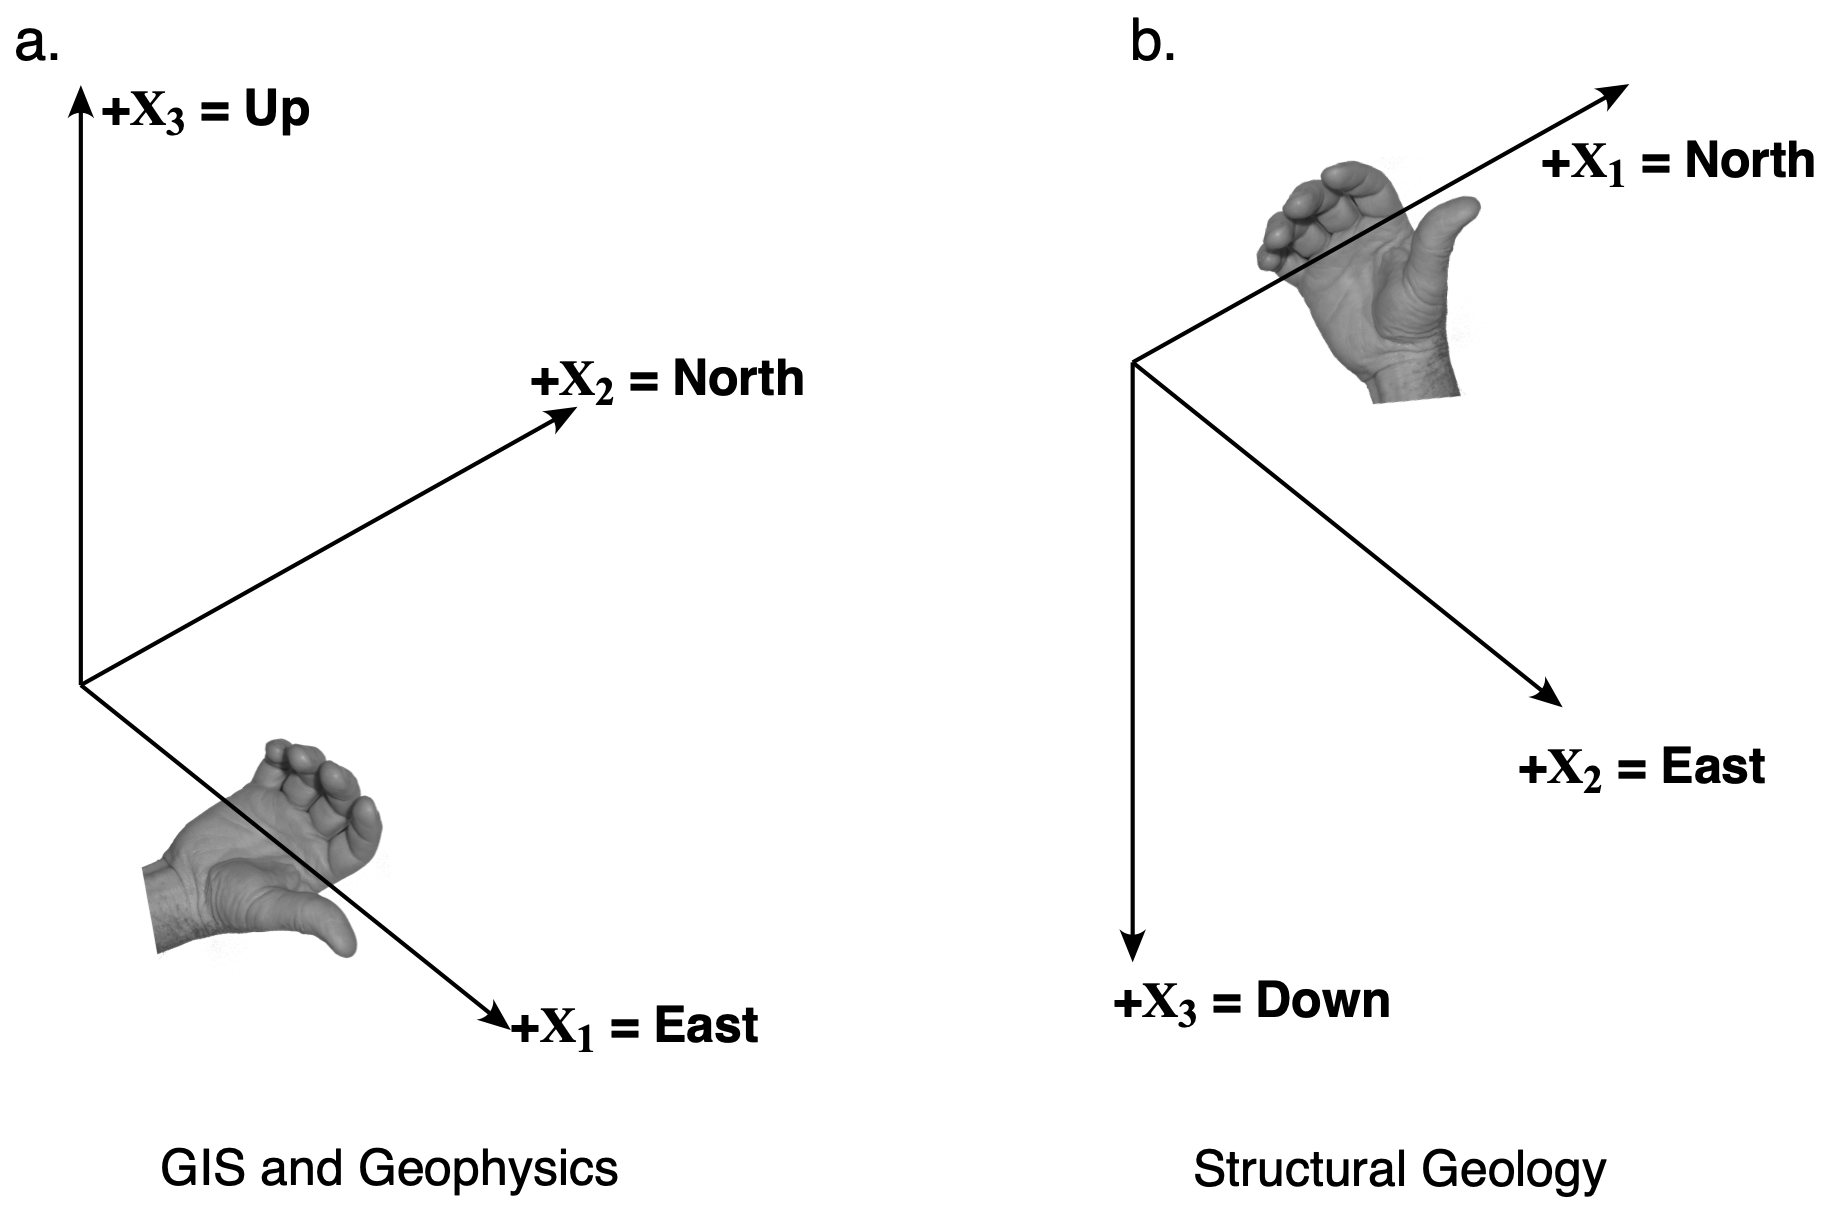
\includegraphics[width=13cm]{Figures/ch4f1.png}
    \caption{Right-handed Cartesian coordinate systems. \textbf{a.} The \textbf{ENU} coordinate system used when dealing with topography, and \textbf{b.} The \textbf{NED} coordinate system used in Structural Geology. Modified from Allmendinger et al. (2012).}
\end{figure}

% SECTION: VECTORS
\section{Vectors}

\subsection{Vector components, magnitude, and unit vectors}
A line from the origin of the Cartesian coordinate system to a point in space is the position \textit{vector} of the point. A \textit{vector} is an object that has both a magnitude and a direction. Displacement, velocity, force, acceleration, and poles to planes, are all vectors. A vector is defined by its three components with respect to the axes of the Cartesian coordinate system; these are the projections of the vector onto the axes $\mathbf{X_1}$, $\mathbf{X_2}$ and $\mathbf{X_3}$ (Fig. 4.2a).

\begin{figure}[ht]
    \centering
    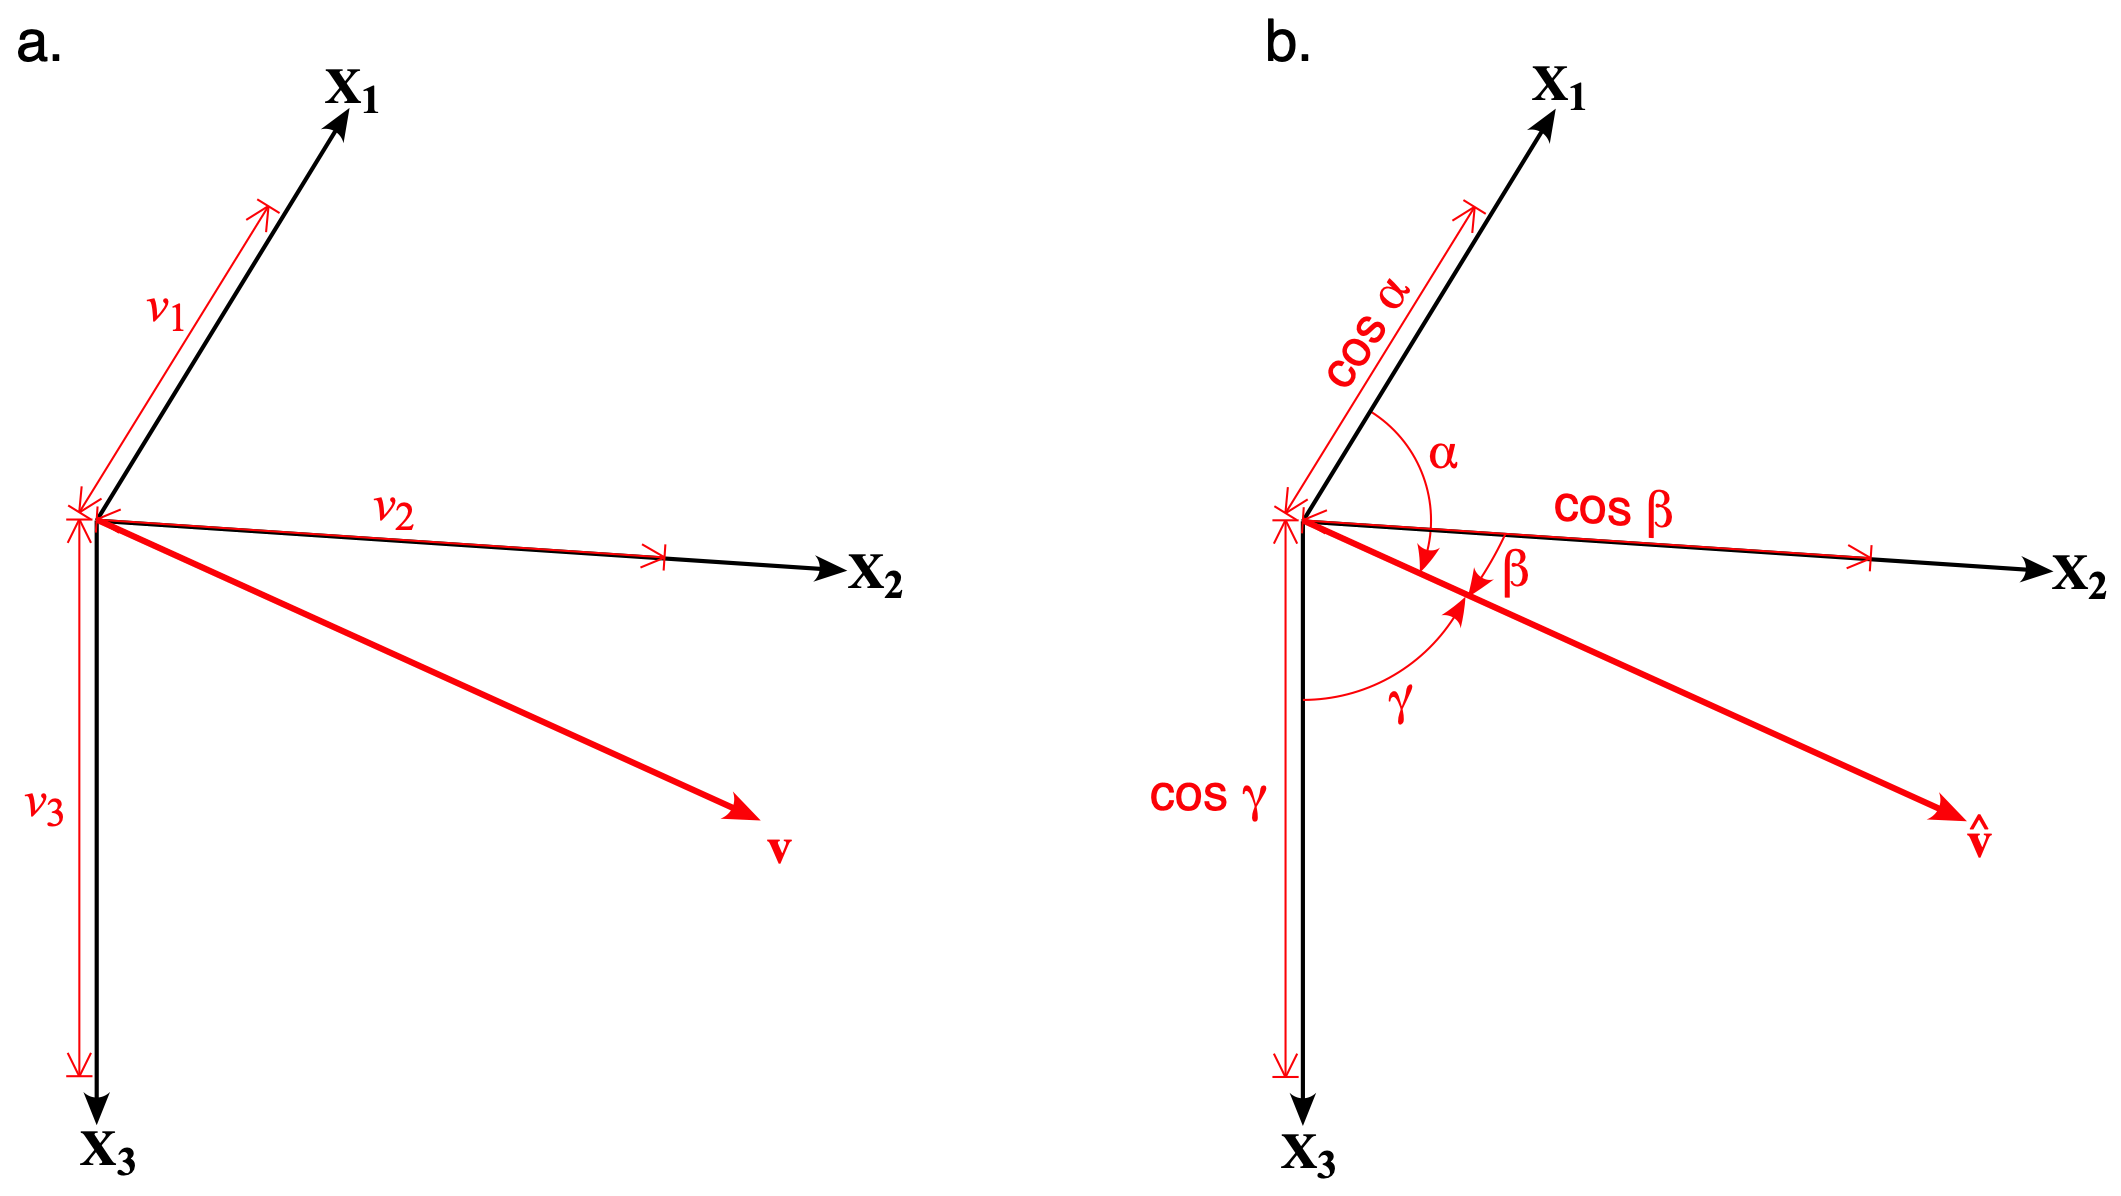
\includegraphics[width=13cm]{Figures/ch4f2.png}
    \caption{\textbf{a.} Components of a vector. \textbf{b.} Direction cosines of a unit vector. Modified from Allmendinger et al. (2012)}
\end{figure}

This is expressed by the following equation:

\begin{equation}
    \mathbf{v} = [v_1,v_2,v_3]
\end{equation}

We use lower capital letters to denote vectors. The magnitude (length) of a vector can be computed using Pythagoras' theorem:
\begin{equation}
    v = (v_1^2+v_2^2+v_3^2)^{1/2}
\end{equation}

The result is just a number, a scalar. We use regular, non-capital letters to denote scalars. If we divide each of the components of a vector by its magnitude, the result is a unit vector, a vector with the same orientation but with a magnitude (length) of one (Fig. 4.2b):

\begin{equation}
    \mathbf{\hat{v}}=[v_1/v,v_2/v,v_3/v]
\end{equation}

We use a hat to indicate unit vectors. There is a very interesting property of unit vectors; the components of a unit vector are the cosines of the angles the vector makes with the axes of the coordinate system (Fig. 4.2b):

\begin{equation}
    \mathbf{\hat v} = [\cos\alpha,\cos\beta,\cos\gamma]
\end{equation}

these are called the \textit{direction cosines} of the vector. By convention, $\cos\alpha$ is the direction cosine of the vector with respect to $\mathbf{X_1}$, $\cos\beta$ is the direction cosine of the vector with respect to $\mathbf{X_2}$, and $\cos\gamma$ is the direction cosine of the vector with respect to $\mathbf{X_3}$ (Fig. 4.2b).

In Python, we can use the NumPy \textit{linalg.norm} function to compute the magnitude of a vector and convert it to a unit vector as illustrated in the following notebook \href{https://github.com/nfcd/compGeo/blob/master/source/notebooks/ch4-1.ipynb}{ch4-1}:

\begin{center}
\begin{lstlisting}[language=Python, frame=single]
# Import numpy
import numpy as np
# Import linear algebra functions
from numpy import linalg as la
# Make vector
v = np.array([1,2,3])
print('Vector: ', v)
# Magnitude of the vector
length = la.norm(v) 
print('Magnitude of the vector: ', length)
# Unit vector
v_hat = v / length
print('Unit Vector: ', v_hat)
# Magnitude of unit vector
length = la.norm(v_hat) 
print('Magnitude of the unit vector: ', length)
\end{lstlisting}
\fbox{
\parbox{\textwidth - 2 \fboxsep}{
Output: \\
Vector:  [1 2 3] \\
Magnitude of the vector:  3.7416573867739413 \\
Unit Vector:  [0.26726124 0.53452248 0.80178373] \\
Magnitude of the unit vector:  1.0
}}   
\end{center}

\subsection{Vector operations}
To multiply a scalar times a vector, just multiply each component of the vector by the scalar:

\begin{equation}
    x\mathbf v=[xv_1,xv_2,xv_3]
\end{equation}

This operation is useful, for example, to reverse the direction of the vector; just multiply the vector by -1.
To add two vectors, just sum their components:

\begin{equation}
    \mathbf u + \mathbf v=\mathbf v+\mathbf u=[u_1+v_1,u_2+v_2,u_3+v_3]
\end{equation}

Vector addition is commutative but vector subtraction is not. Vector addition and subtraction obey the parallelogram rule, whereby the resulting vector bisects the two vectors to be added or subtracted (Fig. 4.3a).

\begin{figure}[ht]
    \centering
    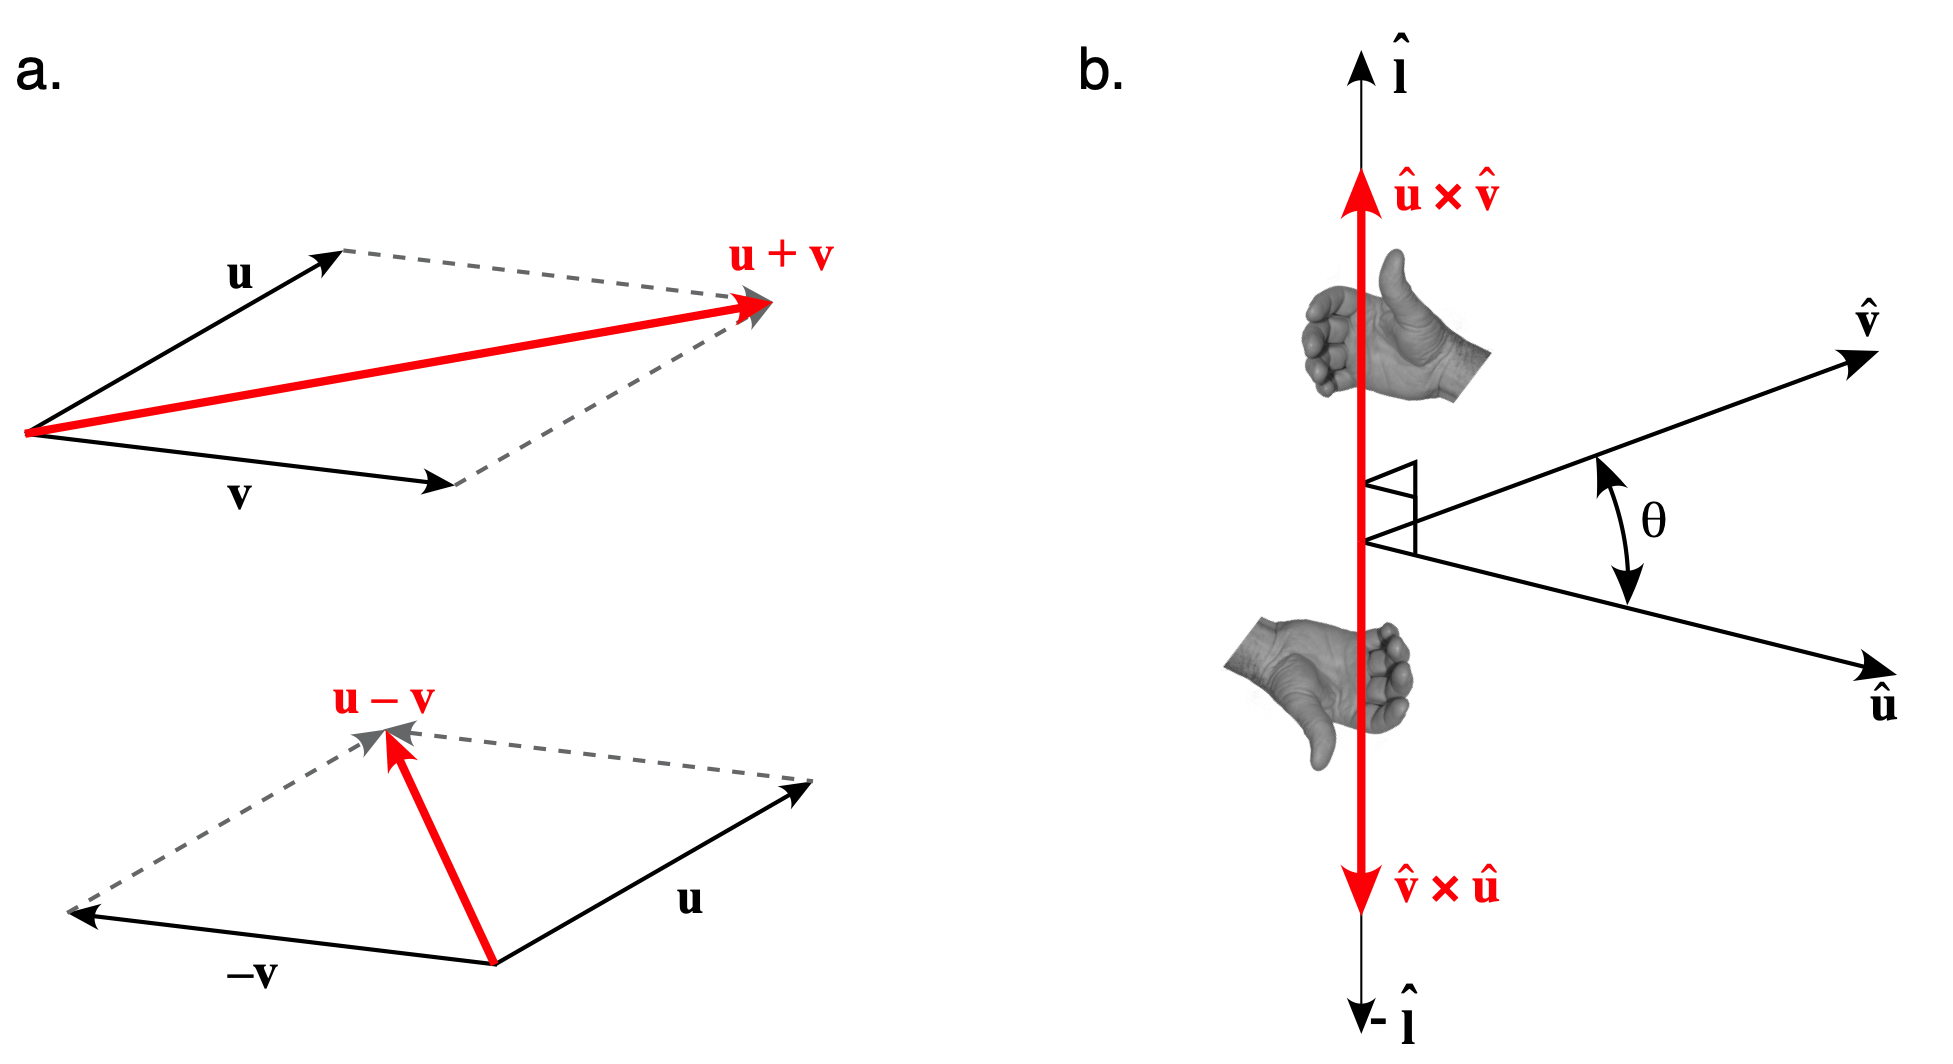
\includegraphics[width=13cm]{Figures/ch4f3.png}
    \caption{\textbf{a.} Vector addition and subtraction. \textbf{b.} Cross product of two unit vectors. Modified from Allmendinger et al. (2012).}
\end{figure}

There are two operations that are unique to vectors: the \textit{dot product} and the \textit{cross product}. The result of the dot product is a scalar and is equal to the magnitude of the first vector times the magnitude of the second vector times the cosine of the angle between the vectors:

\begin{equation}
    \mathbf u \cdot\mathbf v=\mathbf v \cdot\mathbf u=uv\cos\theta=u_1v_1+u_2v_2+u_3v_3=u_iv_i
\end{equation}

The dot product is commutative. If the two vectors are unit vectors, you can easily see that the dot product is:

\begin{equation}
    \mathbf{\hat u} \cdot\mathbf{\hat v}=\cos\theta=u_1v_1+u_2v_2+u_3v_3
\end{equation}

or in terms of the direction cosines of the vectors:

\begin{equation}
    \mathbf{\hat u} \cdot\mathbf{\hat v}=\cos\theta=cos\alpha_1\cos\alpha_2+\cos\beta_1\cos\beta_2+\cos\gamma_1\cos\gamma_2
\end{equation}

which as we will see later, it is a great way to find the angle between two unit vectors.

The result of the cross product is another vector. This vector is perpendicular to the other two vectors, and has a magnitude that is equal to the product of the magnitude of each vector times the sine of the angle between the vectors:

\begin{equation}
    \mathbf u\times\mathbf v=uv\sin\theta\mathbf{\hat l}=[u_2v_3-u_3v_2,u_3v_1-u_1v_3,u_1v_2-u_2v_1]
\end{equation}

The cross product is not commutative. If the vectors are unit vectors, the length of the resulting vector is equal to the sine of the angle between the vectors (Fig. 4.3b). The new vector obeys a right-hand rule; for $\mathbf u\times\mathbf v$, the fingers curl from $\mathbf u$ towards $\mathbf v$ and the thumb points in the direction of the resulting vector, and vice versa (Fig. 4.3b).

In Python, these operations are easy to perform using the NumPy library as shown in the following notebook \href{https://github.com/nfcd/compGeo/blob/master/source/notebooks/ch4-2.ipynb}{ch4-2}:

\begin{center}
\begin{lstlisting}[language=Python, frame=single]
# Import numpy
import numpy as np
# Make vectors
u = np.array([1,2,3])
v = np.array([3,2,1])
print('u = ', u)
print('v = ', v)
# Scalar multiplication of vector
sv = 3 * u
print('3 * u = ', sv)
# Sum of vectors
vsum = u + v
print('u + v = ', vsum)
#  Dot product of vectors
dotp = np.dot(u,v)
print('u . v = ', dotp)
# Cross product of vectors
crossp = np.cross(u,v) 
print('u x v = ', crossp)
\end{lstlisting}
\fbox{
\parbox{\textwidth - 2 \fboxsep}{
Output: \\
u =  [1 2 3] \\
v =  [3 2 1] \\
3 * u =  [3 6 9] \\
u + v =  [4 4 4] \\
u . v =  10 \\
u x v =  [-4  8 -4] \\
}}   
\end{center}

% SECTION: GEOLOGIC FEATURES AS VECTORS
\section{Geologic features as vectors}

We have now all the mathematical tools to represent geologic features as vectors. Since we are only interested in the orientation of these features, we will treat lines and poles to planes as unit vectors. We will also use the Structural Geology \textbf{NED} coordinate system.

\subsection{From spherical to Cartesian coordinates}

Figure 4.4 shows a line as a unit vector $\mathbf{\hat{v}}$ in the \textbf{NED} coordinate system. Clearly, the angle that the line makes with the \textbf{D} axis is 90\degree - \textit{plunge}, therefore:

\begin{figure}[ht]
    \centering
    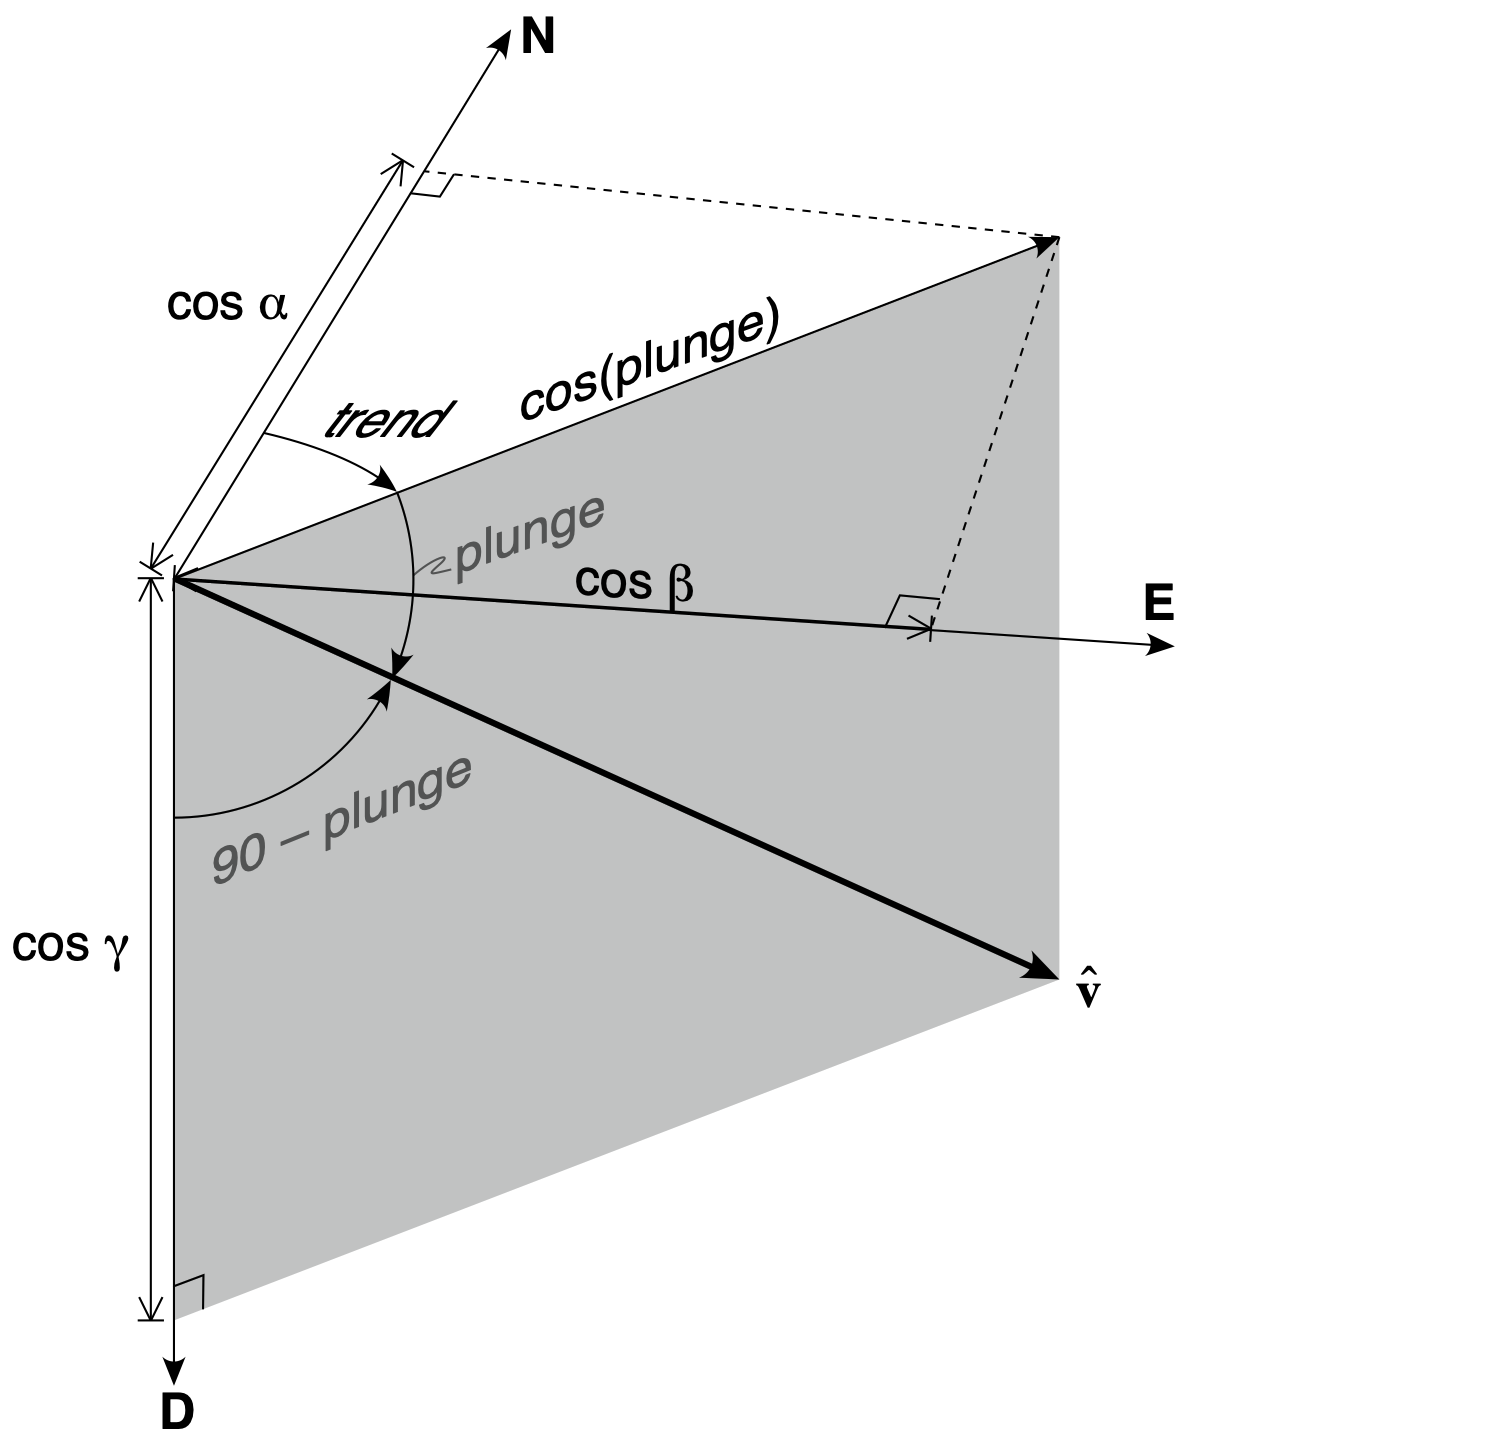
\includegraphics[width=10cm]{Figures/ch4f4.png}
    \caption{Diagram showing the relations between the trend and plunge and the direction cosines in the \textbf{NED} coordinate system. Gray plane is the vertical plane in which the plunge is measured. Modified from Allmendinger et al. (2012).}
\end{figure}

\begin{equation}
    \cos\gamma=\cos(90\degree-plunge)=\sin(plunge) \tag{4.11a}
\end{equation}

The horizontal projection of the line is $\cos(plunge)$ (Fig. 4.4). $\cos\alpha$ and $\cos\beta$ are just the \textbf{N} and \textbf{E} components of this horizontal line (Fig. 4.4):

\begin{equation}
    \cos\alpha=\cos(trend)\cos(plunge) \tag{4.11b}
\end{equation}

\begin{equation}
    \cos\beta=\cos(90\degree-trend)\cos(plunge)=\sin(trend)\cos(plunge) \tag{4.11c}
\end{equation}

The magnitude and sign of the direction cosines tell us a lot about the orientation of the line (Fig. 4.5). A horizontal line (plunge = 0) has $\cos\gamma=0$, a downward pointing line (plunge $>0$) has $+\cos\gamma$, and if the line is vertical (plunge = 90\degree) $\cos\gamma=1$ and the other two direction cosines are 0. A horizontal or downward pointing line (plunge $\geq0$) has $+\cos\alpha$ if it trends NE or NW (first or fourth quadrants), and $+\cos\beta$ if it trends NE or SE (first or second quadrants). If the line trends N or S, $\cos\beta=0$; and if the line trends E or W, $\cos\alpha=0$. 

\begin{figure}[ht]
    \centering
    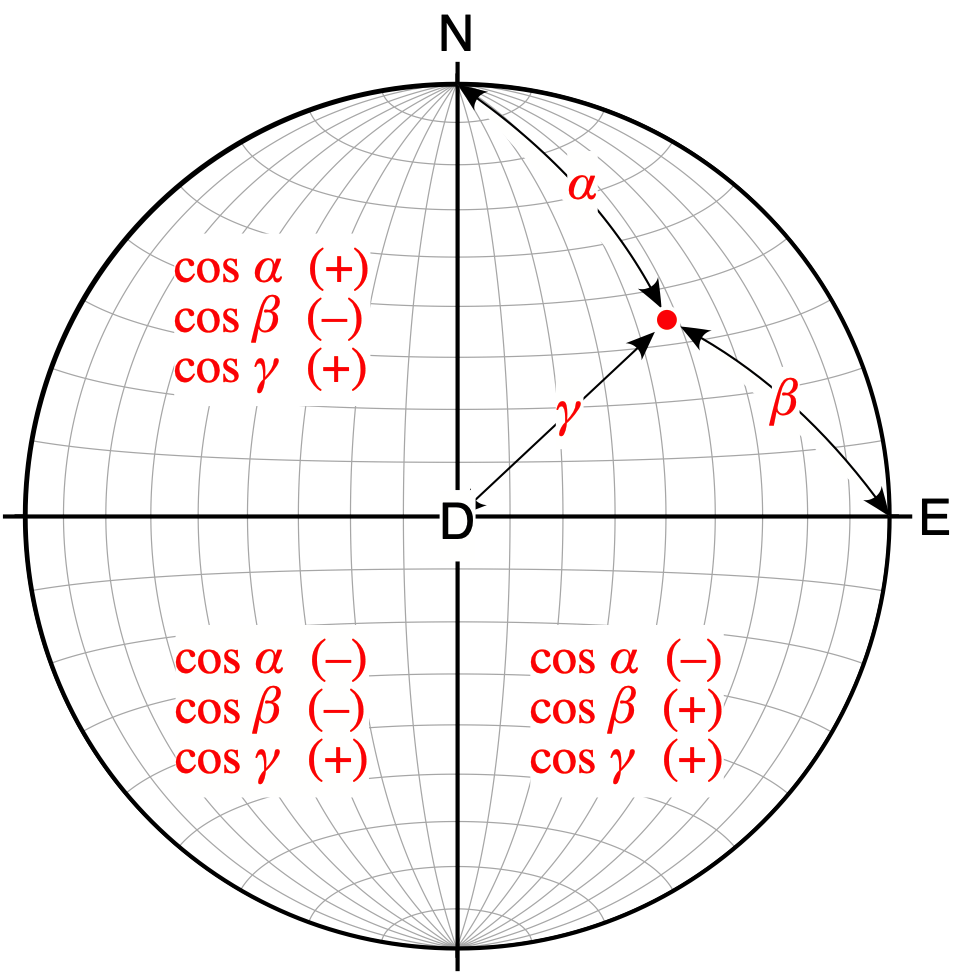
\includegraphics[width=8cm]{Figures/ch4f5.png}
    \caption{Lower hemisphere stereonet showing the sign of the direction cosines in each quadrant. In the NE quadrant, all three direction cosines are positive. Modified from Allmendinger et al. (2012).}
\end{figure}

To determine the direction cosines of a pole to a plane, we just need to express the trend and plunge of the pole in terms of the strike and dip of the plane assuming a RHR format (Eq. 3.2), and use these in Eq. 4.11. The direction cosines of the pole to the plane are then:

\begin{equation}
    \cos\alpha=\cos(strike-90\degree)\cos(90\degree-dip)=\sin(strike)\sin(dip) \tag{4.12a}
\end{equation}

\begin{equation}
     \cos\beta=\sin(strike-90\degree)\cos(90\degree-dip)=-\cos(strike)\sin(dip) \tag{4.12b}
\end{equation}

\begin{equation}
    \cos\gamma=\sin(90\degree-dip)=\cos(dip) \tag{4.12c}
\end{equation}

These equations are summarized in Table 4.1.

\begin{table}[h!]
\small
\centering
\begin{tabular}{p{1.5cm} p{2cm} p{4cm} p{3.5cm}} 
 \hline\hline
 \textbf{Axis} & \textbf{Direction cosines} & \textbf{Lines} & \textbf{Poles to planes}\newline (RHR format) \\ \\
 \hline
 \textbf{N} & $\cos\alpha$ & $\cos(trend)\cos(plunge)$ & $\sin(strike)\sin(dip)$ \\ \\
 \textbf{E} & $\cos\beta$ & $\sin(trend)\cos(plunge)$ & -$\cos(strike)\sin(dip)$ \\ \\
 \textbf{D} & $\cos\gamma$ & $\sin(plunge)$ & $\cos(dip)$ \\
 \hline\hline
\end{tabular}
\caption{Conversion from spherical to Cartesian coordinates}
\label{table4.1}
\end{table}

The following function \href{https://github.com/nfcd/compGeo/blob/master/source/functions/SphToCart.py}{\textit{SphToCart}} converts a line (\textit{k} = 0) or a plane (\textit{k} = 1) from spherical to Cartesian coordinates. Notice that the angles (\textit{trd} and \textit{plg}) should be entered in radians:

\begin{center}
\begin{lstlisting}[language=Python, frame=single]
import math

def SphToCart(trd,plg,k):
    '''
    SphToCart converts from spherical to 
    Cartesian coordinates 

    SphToCart(trd,plg,k) returns the north (cn), 
    east (ce), and down (cd) direction cosines of a line.

    k: integer to tell whether the trend and plunge of a line 
    (k = 0) or strike and dip of a plane in right hand rule 
    (k = 1) are being sent in the trd and plg slots. In this 
    last case, the direction cosines of the pole to the plane 
    are returned
 
    NOTE: Angles should be entered in radians
    
    Python function translated from the Matlab function 
    SphTpCart in Allmendinger et al. (2012)
    '''
    # If line  (see Table 4.1)
    if k == 0:
        cn = math.cos(trd) * math.cos(plg)
        ce = math.sin(trd) * math.cos(plg)  
        cd = math.sin(plg)
    # Else pole to plane (see Table 4.1) 
    elif k == 1:
        cn = math.sin(trd) * math.sin(plg) 
        ce = -math.cos(trd) * math.sin(plg)
        cd = math.cos(plg)
        
    return cn, ce, cd
\end{lstlisting}    
\end{center}

\subsection{From Cartesian to spherical coordinates}

Converting from direction cosines (Cartesian coordinates) to trend and plunge (spherical coordinates) is a little less straightforward. The plunge is easy:

\begin{equation}
    plunge = \sin^{-1}(\cos\gamma) \tag{4.13a}
\end{equation}

The trend can be determined as follows:

\begin{equation*}
    \frac{\cos\beta}{\cos\alpha}=\frac{\sin(trend)\cos(plunge)}{\cos(trend)\cos(plunge)}=\tan(trend)
\end{equation*}

or:

\begin{equation}
    trend = \tan^{-1}\left(\frac{\cos\beta}{\cos\alpha}\right) \tag{4.13b}
\end{equation}

The problem is that the trend varies from 0 and 360\degree. For the $\tan^{-1}$ function, there are two possible angles between 0 and 360\degree. Which one should we use? The answer is to use the signs of the direction cosines to determine in which quadrant the trend lies within. By inspection of Figure 4.5, one can see that:

\begin{equation}
    trend = \tan^{-1}\left(\frac{\cos\beta}{\cos\alpha}\right)\,\,if\,\cos\alpha>0 \tag{4.14a}
\end{equation}

\begin{equation}
    trend = 180\degree+\tan^{-1}\left(\frac{\cos\beta}{\cos\alpha}\right)\,\,if\,\cos\alpha<0 \tag{4.14b}
\end{equation}

One should also check for the special case of $\cos\alpha=0$:

\begin{equation}
    trend = 90\degree\,\,if\,(\cos\alpha = 0\,\,and\,\cos(\beta)\geq 0) \tag{4.14c}
\end{equation}

\begin{equation}
    trend = 270\degree\,\,if\,(\cos\alpha = 0\,\,and\,\cos(\beta)< 0) \tag{4.14d}
\end{equation}

The following function \href{https://github.com/nfcd/compGeo/blob/master/source/functions/CartToSph.py}{\textit{CartToSph}} converts a line from Cartesian to spherical coordinates. Notice that the trend and plunge are returned in radians:

\begin{center}
\begin{lstlisting}[language=Python, frame=single]
import math
from ZeroTwoPi import ZeroTwoPi as ZeroTwoPi

def CartToSph(cn,ce,cd):
    '''
    CartToSph converts from Cartesian to spherical coordinates 

    CartToSph(cn,ce,cd) returns the trend (trd)
    and plunge (plg) of a line for input north (cn), 
    east (ce), and down (cd) direction cosines

    NOTE: Trend and plunge are returned in radians

    CartToSph uses function ZeroTwoPi
    
    Python function translated from the Matlab function 
    CartToSph in Allmendinger et al. (2012)
    '''
    pi = math.pi
    # Plunge 
    plg = math.asin(cd) # Eq. 4.13a
    
    #Trend
    #If north direction cosine is zero, trend is east or west
    #Choose which one by the sign of the east direction cosine
    if cn == 0.0:
        if ce < 0.0:
            trd = 3.0/2.0*pi # Eq. 4.14d, trend is west
        else:
            trd = pi/2.0 # Eq. 4.14c, trend is east
    # Else
    else:
        trd = math.atan(ce/cn) # Eq. 4.14a
        if cn < 0.0:
            #Add pi 
            trd = trd+pi # Eq. 4.14b
        # Make sure trd is between 0 and 2*pi
        trd = ZeroTwoPi(trd)
    
    return trd, plg
\end{lstlisting}    
\end{center}

% SECTION: APPLICATIONS
\section{Applications}

\subsection{Mean vector}

An important problem in geosciences is to determine the average or mean vector that represents a group of lines. These lines can be for example poles to bedding, paleocurrent directions, paleomagnetic poles, or slip vectors on a fault surface. This problem can be solved using vector addition. The resultant vector $\mathbf{r}$ of the sum of the \textit{N} unit vectors representing the lines has components:

\begin{equation}
    r_1=\sum_{i=1}^{N}\alpha_i\qquad r_2=\sum_{i=1}^{N}\beta_i\qquad r_3=\sum_{i=1}^{N}\gamma_i \tag{4.15a}
\end{equation}

where $\alpha$, $\beta$ and $\gamma$ are the direction cosines of the unit vectors. The length of the resultant vector $\mathbf{r}$ is:

\begin{equation}
    r=\sqrt{r_1^2+r_2^2+r_3^2} \tag{4.15b}
\end{equation}

and the direction cosines of the unit vector that is parallel to the mean of the individual vectors are:

\begin{equation}
    \overline{\alpha}=\frac{r_1}{r}\qquad \overline{\beta}=\frac{r_2}{r}\qquad \overline{\gamma}=\frac{r_3}{r} \tag{4.15c}
\end{equation}

These direction cosines define the orientation of the mean vector. A measure of how concentrated the individual vectors are or how representative the mean vector is, is given by the \textit{mean resultant length}:

\begin{equation}
    \overline{r}=\frac{r}{N}\qquad where\qquad 0\leq\overline{r}\leq 1 \tag{4.15d}
\end{equation}

The closer this value is to 1, the better the concentration. The function \href{https://github.com/nfcd/compGeo/blob/master/source/functions/CalcMV.py}{\textit{CalcMV}} calculates the mean vector for a series of lines. It also calculates the Fisher statistics for the mean vector (Fisher et al., 1987), which is the standard way to represent uncertainties in this analysis. Notice that \textit{CalcMV} uses our two previous functions \textit{SphToCart} and \textit{CartToSph} to convert from spherical to Cartesian coordinates, and vice versa.

\begin{center}
\begin{lstlisting}[language=Python, frame=single]
import math
from SphToCart import SphToCart as SphToCart
from CartToSph import CartToSph as CartToSph

def CalcMV(T, P):
    '''
    CalcMV calculates the mean vector for a group of lines

    CalcMV(T,P) calculates the trend (trd) and plunge (plg) 
    of the mean vector, its mean resultant length (Rave), and
    Fisher statistics (concentration factor (conc), 99 (d99) 
    and 95 (d95) % uncertainty cones); for a series of lines 
    whose trends and plunges are stored in the arrays T and P

    NOTE: Input/Output trends and plunges, as well as 
    uncertainty cones are in radians

    CalcMV uses functions SphToCart and CartToSph
    
    Python function translated from the Matlab function 
    CalcMV in Allmendinger et al. (2012)
    '''
    # Number of lines
    nlines = len(T) 
    
    # Initialize the 3 direction cosines which contain the 
    # sums of the individual vectors 
    CNsum = 0.0
    CEsum = 0.0
    CDsum = 0.0
    
    #Now add up all the individual vectors. Eq. 4.15a
    for i in range(nlines):
        cn,ce,cd = SphToCart(T[i],P[i],0)
        CNsum += cn
        CEsum += ce
        CDsum += cd
    
    # R is the length of the resultant vector and 
    # Rave is the mean resultant length. Eqs. 4.15b and d
    R = math.sqrt(CNsum*CNsum + CEsum*CEsum + CDsum*CDsum)
    Rave = R/nlines
    # If Rave is lower than 0.1, the mean vector is 
    # insignificant, return error
    if Rave < 0.1:
        raise ValueError('Mean vector is insignificant')
    #Else 
    else:
        # Divide the resultant vector by its length to get 
        # the direction cosines of the unit vector
        CNsum = CNsum/R
        CEsum = CEsum/R
        CDsum = CDsum/R
        # Convert the mean vector to the lower hemisphere
        if CDsum < 0.0:
            CNsum = -CNsum
            CEsum = -CEsum
            CDsum = -CDsum
        # Convert the mean vector to trend and plunge
        trd, plg = CartToSph(CNsum,CEsum,CDsum)
        # If there are enough measurements calculate the 
        # Fisher statistics (Fisher et al., 1987)
        if R < nlines:
            if nlines < 16:
                afact = 1.0-(1.0/nlines)
                conc = (nlines/(nlines-R))*afact**2
            else:
                conc = (nlines-1.0)/(nlines-R)
        if Rave >= 0.65 and Rave < 1.0:
            afact = 1.0/0.01
            bfact = 1.0/(nlines-1.0)
            d99 = math.acos(1.0-((nlines-R)/R)*(afact**bfact-1.0))
            afact = 1.0/0.05
            d95 = math.acos(1.0-((nlines-R)/R)*(afact**bfact-1.0))
    
    return trd, plg, Rave, conc, d99, d95
\end{lstlisting}    
\end{center}

The notebook \href{https://github.com/nfcd/compGeo/blob/master/source/notebooks/ch4-3.ipynb}{ch4-3} shows the solution to the mean vector problem in Ragan (2009, pp. 147-148), which involves finding the mean orientation of 10 poles to bedding:

\begin{center}
\begin{lstlisting}[language=Python, frame=single]
import numpy as np
import matplotlib.pyplot as plt
%matplotlib inline

import sys
import os
sys.path.append(os.path.abspath('../functions'))
from StCoordLine import StCoordLine as StCoordLine
from CalcMV import CalcMV as CalcMV 

# Arrays T and P contain the trend (T) 
# and plunge (P) of the 10 poles
T = np.array([206, 220, 204, 198, 200, 188, 192, 228, 236, 218])
P = np.array([32, 30, 46, 40, 20, 32, 54, 56, 36, 44])

# Convert T and P from degrees to radians
pi = np.pi
TR = T * pi/180
PR = P * pi/180

# Compute the mean vector and print orientation
# and mean resultant length
trd, plg, Rave, conc, d99, d95 = CalcMV(TR,PR)
print('Mean vector trend = {:.1f}, plunge {:.1f}'.format(trd*180/pi,plg*180/pi))
print('Mean resultant length = {:.3f}'.format(Rave))

# Plot the primitive of the stereonet
r = 1; # unit radius
TH = np.arange(0,360,1)*pi/180
x = r * np.cos(TH)
y = r * np.sin(TH)
plt.plot(x,y,'k')
# Plot center of circle
plt.plot(0,0,'k+')
# Make axes equal and remove them
plt.axis('scaled')
plt.axis('off')

# Plot the poles as black points
# on an equal angle stereonet
npoles = len(T)
eqAngle = np.zeros((npoles, 2))
for i in range(npoles):
    # Equal angle coordinates
    eqAngle[i,0], eqAngle[i,1] = StCoordLine(TR[i],PR[i],0)
plt.plot(eqAngle[:,0],eqAngle[:,1],'ko')

# Plot the mean vector as a red point
mvx, mvy = StCoordLine(trd,plg,0)
plt.plot(mvx,mvy,'ro')
\end{lstlisting}
\fbox{
    \parbox{\textwidth - 2 \fboxsep}{
    Output: \\
    Mean vector trend = 208.6, plunge 40.0 \\
    Mean resultant length = 0.963 \\
    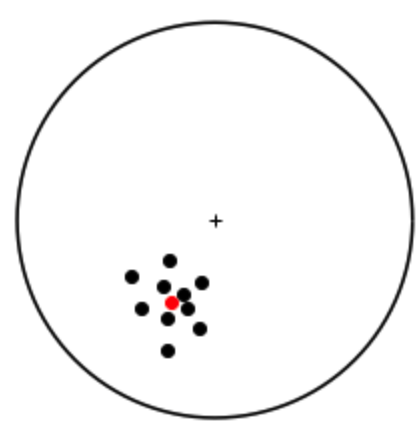
\includegraphics[width=4.75cm]{Figures/ch4f6.png}
}}
\end{center}

Notice that the mean resultant length is 0.963, so that the mean vector (red dot) is a representative orientation of the individual vectors (black dots).

\subsection{Angles, intersections, and poles}

Many interesting problems can be solved using the dot and cross product operations. The dot product can be used to find the angle between two lines or planes, while the cross product can be used to find a plane from two lines or the intersection of two planes. Table 4.2 lists some problems that can be solved using these operations.

\begin{table}[h!]
\small
\centering
\begin{tabular}{ | p{6cm} | p{6cm} | } 
 \hline
 \multicolumn{1}{|c|}{Problem} & \multicolumn{1}{|c|}{Solution}  \\
 \hline
 Angle between two lines & $\arccos$ of dot product between lines \\
 \hline
 Angle between two planes & supplement of $\arccos$ of dot product between poles to planes \\
 \hline
 Intersection of two planes & Cross product of poles to planes \\
 \hline
 Plane containing two lines & Pole to plane is cross product of lines \\
 \hline
 Apparent dip of plane & Intersection of plane and vertical section of a given orientation \\
 \hline
 Plane from two apparent dips & Plane containing the two apparent dips (lines) \\
 \hline
\end{tabular}
\caption{Some problems that can be solved using the dot and cross product operations.}
\label{table4.2}
\end{table}

The function \href{https://github.com/nfcd/compGeo/blob/master/source/functions/Angles.py}{\textit{Angles}} computes the angle between two lines (\textit{ans0} = \textit{'l'}), the angle between two planes (\textit{ans0} = \textit{'p'}), the plane from two lines (\textit{ans0} = \textit{'a'}), or the intersection of two planes (\textit{ans0} = \textit{'i'}).

\begin{center}
\begin{lstlisting}[language=Python, frame=single]
import math
from SphToCart import SphToCart as SphToCart
from CartToSph import CartToSph as CartToSph
from Pole import Pole as Pole

def Angles(trd1,plg1,trd2,plg2,ans0):
    '''
    Angles calculates the angles between two lines, 
    between two planes, the line which is the intersection 
    of two planes, or the plane containing two apparent dips

    Angles(trd1,plg1,trd2,plg2,ans0) operates on
    two lines or planes with trend/plunge or 
    strike/dip equal to trd1/plg1 and trd2/plg2

    ans0 is a character that tells the function what 
    to calculate:

      ans0 = 'a' -> plane from two apparent dips
      ans0 = 'l' -> the angle between two lines

      In the above two cases, the user sends the trend 
      and plunge of two lines

      ans0 = 'i' -> the intersection of two planes
      ans0 = 'p' -> the angle between two planes
 
      In the above two cases the user sends the strike 
      and dip of two planes in RHR format

    NOTE: Input/Output angles are in radians

    Angles uses functions SphToCart, CartToSph and Pole

    Python function translated from the Matlab function 
    Angles in Allmendinger et al. (2012)
    '''
    # If planes have been entered
    if ans0 == 'i' or ans0 == 'p':
        k = 1
    # Else if lines have been entered
    elif ans0 == 'a' or ans0 == 'l':
        k = 0
    
    # Calculate the direction cosines of the lines 
    # or poles to planes
    cn1, ce1, cd1 = SphToCart(trd1,plg1,k)
    cn2, ce2, cd2 = SphToCart(trd2,plg2,k)
    
    # If angle between 2 lines or between 
    # the poles to 2 planes
    if ans0 == 'l' or ans0 == 'p':
        # Use dot product 
        ans1 = math.acos(cn1*cn2 + ce1*ce2 + cd1*cd2)
        ans2 = math.pi - ans1
    
    # If intersection of two planes or pole to 
    # a plane containing two apparent dips
    if ans0 == 'a' or ans0 == 'i':
        # If the 2 planes or lines are parallel 
        # return an error
        if trd1 == trd2 and plg1 == plg2:
            raise ValueError('Error: lines or planes are parallel')
        # Else use cross product
        else:
            cn = ce1*cd2 - cd1*ce2
            ce = cd1*cn2 - cn1*cd2
            cd = cn1*ce2 - ce1*cn2
            #Make sure the vector points downe
            if cd < 0.0:
                cn = -cn
                ce = -ce
                cd = -cd
            # Convert vector to unit vector
            r = math.sqrt(cn*cn+ce*ce+cd*cd)
            # Calculate line of intersection or pole to plane
            trd, plg = CartToSph(cn/r,ce/r,cd/r)
            # If intersection of two planes
            if ans0 == 'i':
                ans1 = trd
                ans2 = plg
            # Else if plane containing two dips, 
            # calculate plane from its pole
            elif ans0 == 'a':
                ans1, ans2 = Pole(trd,plg,0)
    
    return ans1, ans2
\end{lstlisting}    
\end{center}

The notebook \href{https://github.com/nfcd/compGeo/blob/master/source/notebooks/ch4-4.ipynb}{ch4-4} illustrates the use of the function \textit{Angles} to solve several interesting problems. Let's start with the following problem from Leyshon and Lisle (1996): Two limbs of a chevron fold (A and B) have orientations (RHR) as follows: Limb A = 120/40, Limb B = 250/60. Determine: (a) the trend and plunge of the hinge line of the fold, (b) the rake of the hinge line in limb A, (c) the rake of the hinge line in limb B. 

\begin{center}
\begin{lstlisting}[language=Python, frame=single]
import math
pi = math.pi

import sys
import os
sys.path.append(os.path.abspath('../functions'))
from Angles import Angles as Angles

# Strike and dip of the limbs in radians
str1 = 120 * pi/180 # SW dipping limb
dip1 = 40 * pi/180
str2 = 250 * pi/180 # NE dipping limb
dip2 = 60 * pi/180

# (a) Chevron folds have planar limbs. The hinge
# of the fold is the intersection of the limbs
htrd, hplg = Angles(str1,dip1,str2,dip2,'i')
print('Hinge trend = {:.1f}, plunge {:.1f}'.format(htrd*180/pi,hplg*180/pi))

# The rake of the hinge on either limb is the angle 
# between the hinge and the strike line on the limb. 
# This line is horizontal and has plunge = 0
plg = 0

# (b) For the SW dipping limb
ang1, ang2 = Angles(str1,plg,htrd,hplg,'l')
print('Rake of hinge in SW dipping limb = {:.1f}'.format(ang1*180/pi))

# (c) And for the NE dipping limb
ang1, ang2 = Angles(str2,plg,htrd,hplg,'l')
print('Rake of hinge in NE dipping limb = {:.1f}'.format(ang1*180/pi))
\end{lstlisting}
\fbox{
    \parbox{\textwidth - 2 \fboxsep}{
    Output: \\
    Hinge trend = 265.8, plunge 25.3 \\
    Rake of hinge in SW dipping limb = 138.4 \\
    Rake of hinge in NE dipping limb = 29.5 \\
}}
\end{center}

Let's do another problem from the same book: A quarry has two walls, one trending 002\degree and the other 135\degree. The apparent dip of bedding on the faces are 40\degree N and 30\degree SE respectively. Calculate the strike and dip of bedding.

\begin{center}
\begin{lstlisting}[language=Python, frame=single]
# The apparent dips are just two lines on bedding
# These lines have orientations:
trd1 = 2 * pi/180
plg1 = 40 * pi/180
trd2 = 135 * pi/180
plg2 = 30 * pi/180

# Calculate bedding from these two apparent dips
strike, dip = Angles(trd1,plg1,trd2,plg2,'a')
print('Bedding strike = {:.1f}, dip {:.1f}'.format(strike*180/pi,dip*180/pi))
\end{lstlisting}
\fbox{
    \parbox{\textwidth - 2 \fboxsep}{
    Output: \\
    Bedding strike = 333.9, dip 60.7
}}
\end{center}

And the final problem also from the same book: Slickenside lineations trending 074\degree occur on a fault with orientation 300/50 (RHR). Determine the plunge of these lineations and their rake in the plane of the fault.

\begin{center}
\begin{lstlisting}[language=Python, frame=single]
# The lineation on the fault is just the intersection
# of a vertical plane with a strike equal to
# the trend of the lineation, and the fault
str1 = 74 * pi/180
dip1 = 90 * pi/180
str2 = 300 * pi/180
dip2 = 50 * pi/180

# Find the intersection of these two planes which is
# the lineation on the fault
ltrd, lplg = Angles(str1,dip1,str2,dip2,'i')
print('Slickensides trend = {:.1f}, plunge {:.1f}'.format(ltrd*180/pi,lplg*180/pi))

# And the rake of this lineation is the angle
# between the lineation and the strike line on the fault
plg = 0
ang1, ang2 = Angles(str2,plg,ltrd,lplg,'l')
print('Rake of slickensides = {:.1f}'.format(ang1*180/pi))
\end{lstlisting}
\fbox{
    \parbox{\textwidth - 2 \fboxsep}{
    Output: \\
    Slickensides trend = 74.0, plunge 40.6 \\
    Rake of slickensides = 121.8 \\
}}
\end{center}

There are many interesting problems you can solve using the function \textit{Angles}. You will find more problems in section \ref{exercises4}.

\subsection{Three point problem}

The three point problem is a fundamental problem in geology. It derives from the fact that three non-collinear points on a plane define the orientation of the plane. The graphical solution to this problem is introduced early in the Geosciences Bachelor. It involves finding the strike line (a line connecting two points of equal elevation) on the plane, and the dip from two strike lines (two structure contours) on the plane. 

There is however an easier and more accurate solution to this problem using linear algebra: The three points on the plane define two lines, and the cross product between these lines is parallel to the pole to the plane, from which the orientation of the plane can be estimated. The function \href{https://github.com/nfcd/compGeo/blob/master/source/functions/ThreePoint.py}{\textit{ThreePoint}} computes the strike and dip of plane from the east (\textbf{E}), north (\textbf{N}), and up (\textbf{U}) coordinates of three points on the plane:

\begin{lstlisting}[language=Python, frame=single]
import numpy as np
from numpy import linalg as la
from CartToSph import CartToSph as CartToSph
from Pole import Pole as Pole

def ThreePoint(p1,p2,p3):
    '''
    ThreePoint calculates the strike (strike) and dip (dip) 
    of a plane given the east (E), north (N), and up (U) 
    coordinates of three non-collinear points on the plane
    
    p1, p2 and p3 are 1 x 3 arrays defining the location 
    of the points in an ENU coordinate system. For each one 
    of these arrays the first entry is the E coordinate, 
    the second entry the N coordinate, and the third entry 
    the U coordinate

    NOTE: strike and dip are returned in radians and they 
    follow the right-hand rule format

    ThreePoint uses functions CartToSph and Pole
    '''
    # make vectors v (p1 - p3) and u (p2 - p3)
    v = p1 - p2
    u = p2 - p3
    
    # take the cross product of v and u
    vcu = np.cross(v,u)
    
    # make this vector a unit vector
    mvcu = la.norm(vcu) # magnitude of the vector
    uvcu = vcu/mvcu # unit vector
    
    # make the pole vector in NED coordinates
    p = [uvcu[1], uvcu[0], -uvcu[2]]

    # Make pole point downwards
    if p[2] < 0:
        p = [-elem for elem in p]
        
    # find the trend and plunge of the pole
    trd, plg = CartToSph(p[0],p[1],p[2])
    
    # find strike and dip of plane
    strike, dip = Pole(trd,plg,0)
    
    return strike , dip
\end{lstlisting}

Let's use this function in the following example. The geologic map in Fig. 4.6 shows a sequence of sedimentary units dipping south (you can see this by the outcrop V in the valley). Points 1, 2 and 3 are located on the base of unit S and their \textbf{ENU} coordinates are: 

point1 = [509, 2041, 400]

point2 = [1323, 2362, 500]

point3 = [2003, 2913, 700] 

Calculate the strike and dip of the plane. The Python notebook \href{https://github.com/nfcd/compGeo/blob/master/source/notebooks/ch4-5.ipynb}{ch4-5} shows the solution to this problem:\\ 

\begin{figure}[ht]
    \centering
    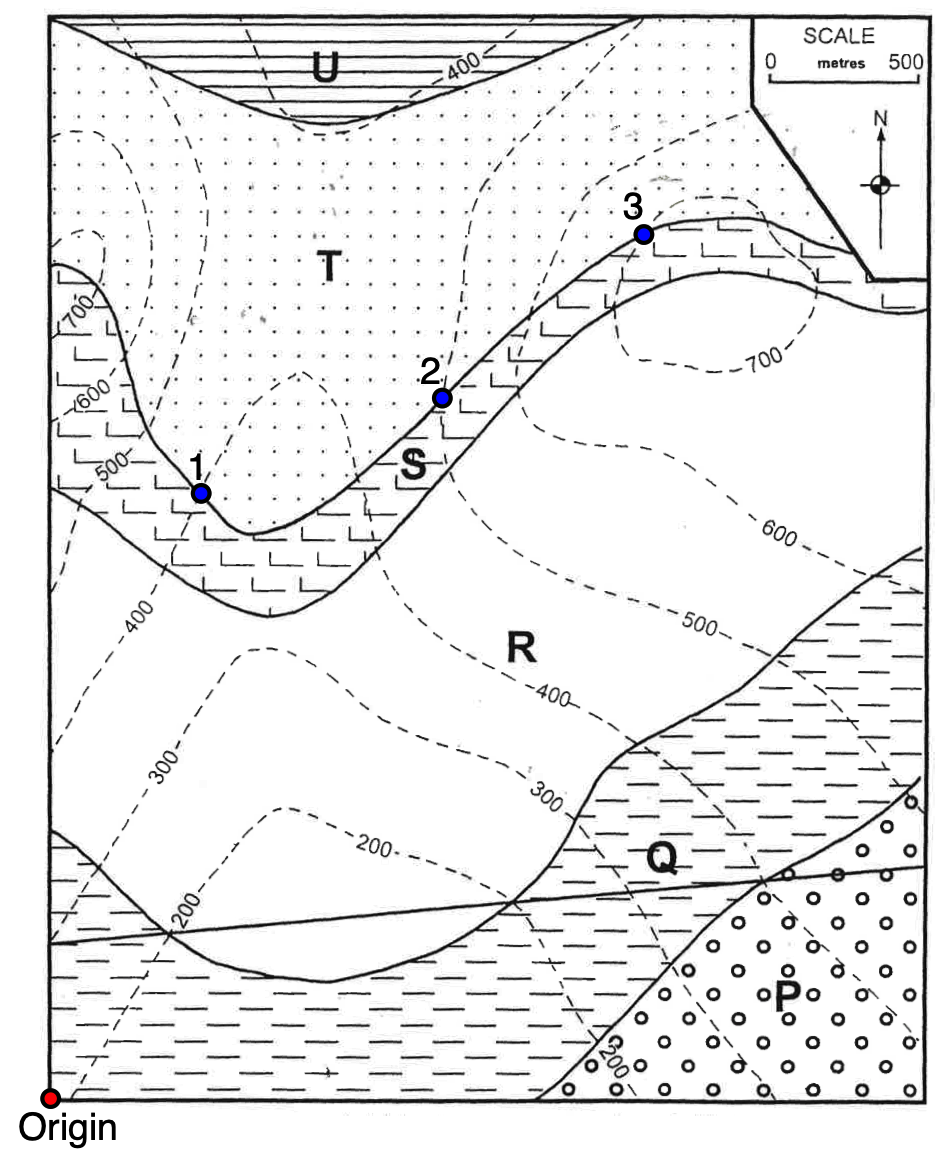
\includegraphics[width=9cm]{Figures/ch4f7.png}
    \caption{Geologic map of sedimentary units dipping south (Bennison et al., 2011). Points 1 to 3 on the base of unit S are used to estimate the orientation of bedding. Notice that the origin is at the lower left corner.}
\end{figure}

\begin{center}
\begin{lstlisting}[language=Python, frame=single]
import numpy as np
pi = np.pi

import sys
import os
sys.path.append(os.path.abspath('../functions'))
from ThreePoint import ThreePoint as ThreePoint

# ENU coordinates of the three points
p1 = np.array([509, 2041, 400])
p2 = np.array([1323, 2362, 500])
p3 = np.array([2003, 2913, 700])

# Compute the orientation of the plane
strike, dip = ThreePoint(p1,p2,p3)
print('Plane strike = {:.1f}, dip = {:.1f}'.format(strike*180/pi,dip*180/pi))
\end{lstlisting}
\fbox{
    \parbox{\textwidth - 2 \fboxsep}{
    Output: \\
    Plane strike = 84.5, dip = 22.5
}}
\end{center}

% SECTION: Uncertainties
\section{Uncertainties}\label{calcuncertainties}

As we saw in section \ref{uncertainties}, strike and dip or trend and plunge measurements have errors (Figs. 3.6 and 3.7), and these errors  propagate in any computation making use of these angles. Also, as accurate as GPS and elevation measurements are today, they also have errors. Thus, functions \textit{Angles} and \textit{ThreePoint} lack this important element of uncertainty.

Suppose that \textit{x, ..., z} are measured with uncertainties (or errors) \textit{$\delta x$, ..., $\delta z$} and the measured values are used to compute the function $q(x,...,z)$. If the uncertainties in \textit{x, ..., z} are independent and random, then the uncertainty (or error) in \textit{q} is (Taylor, 1997):

\begin{equation}
    \delta q=\sqrt{\left(\frac{\partial q}{\partial x}\delta x \right)^2+...+\left(\frac{\partial q}{\partial z}\delta z \right)^2}\tag{4.16}
\end{equation}

This formula is easy to calculate for a few operations, but it can become quite complex for a long chain of operations. Fortunately, there is a Python package that handles calculations with numbers with uncertainties. This package is called \textit{uncertainties} and it was developed by Eric Lebigot. You can find details about the package as well as instructions for installing it in the \href{https://pythonhosted.org/uncertainties/}{uncertainties} website. If you have the Python \textit{pip} package-management system, you can install the uncertainties package by entering in a terminal:

\begin{center}
\begin{lstlisting}[language=Python, frame=single]
pip install --upgrade uncertainties
\end{lstlisting}
\end{center}

After this, you can use the uncertainties package in your functions. The functions \href{https://github.com/nfcd/compGeo/blob/master/source/functions/AnglesU.py}{\textit{AnglesU}} and \href{https://github.com/nfcd/compGeo/blob/master/source/functions/ThreePointU.py}{\textit{ThreePointU}} in the resource git repository, are the corresponding \textit{Angles} and \textit{ThreePoint} functions with uncertainties. We don't list these functions here, but rather illustrate their use in the following notebook \href{https://github.com/nfcd/compGeo/blob/master/source/notebooks/ch4-6.ipynb}{ch4-6}.

In the first problem on page 64, the uncertainty in strike is 4\degree and in dip is 2\degree. What is the uncertainty in the hinge orientation and its rake on the limbs? This problem can be solved as follows:

\begin{center}
\begin{lstlisting}[language=Python, frame=single]
import numpy as np
pi = np.pi
import uncertainties as unc

import sys
import os
sys.path.append(os.path.abspath('../functions'))
from AnglesU import AnglesU as AnglesU

# Strike and dip of the limbs in radians
str1 = 120 * pi/180 # SW dipping limb
dip1 = 40 * pi/180
str2 = 250 * pi/180 # NE dipping limb
dip2 = 60 * pi/180

# Errors in radians
ustr = 4 * pi/180 # Error in strike
udip = 2 * pi/180 # Error in dip

# Create the input values with uncertainties
str1 = unc.ufloat(str1, ustr)  # str1 = str1 +/-ustr
dip1 = unc.ufloat(dip1, udip)  # dip1 = dip1 +/-udip
str2 = unc.ufloat(str2, ustr)  # str2 = str2 +/-ustr
dip2 = unc.ufloat(dip2, udip)  # dip2 = dip2 +/-udip

# (a) Chevron folds have planar limbs. The hinge
# of the fold is the intersection of the limbs
htrd, hplg = AnglesU(str1,dip1,str2,dip2,'i')
print('Hinge trend = {:.1f}, plunge {:.1f}'.format(htrd*180/pi,hplg*180/pi))

# The rake of the hinge on either limb is the angle 
# between the hinge and the strike line on the limb. 
# This line is horizontal and has plunge = 0
plg = unc.ufloat(0, udip)  # plg = 0 +/-udip

# (b) For the SW dipping limb
ang1, ang2 = AnglesU(str1,plg,htrd,hplg,'l')
print('Rake of hinge in SW dipping limb = {:.1f}'.format(ang1*180/pi))

# (c) And for the NE dipping limb
ang1, ang2 = AnglesU(str2,plg,htrd,hplg,'l')
print('Rake of hinge in NE dipping limb = {:.1f}'.format(ang1*180/pi))
\end{lstlisting}
\fbox{
    \parbox{\textwidth - 2 \fboxsep}{
    Output: \\
    Hinge trend = 265.8+/-3.3, plunge 25.3+/-2.6 \\
    Rake of hinge in SW dipping limb = 138.4+/-4.6 \\
    Rake of hinge in NE dipping limb = 29.5+/-3.5 \\
}}
\end{center}

In the map of Fig. 4.6, the error in east and north coordinates is 10 m, and in elevation is 5 m. What is uncertainty in the strike and dip of the T-S contact? 

\begin{center}
\begin{lstlisting}[language=Python, frame=single]
from ThreePointU import ThreePointU as ThreePointU

# ENU coordinates of the three points
# with uncertainties in E-N = 10, and U = 5
p1 = np.array([unc.ufloat(509, 10), unc.ufloat(2041, 10), unc.ufloat(400, 5)])
p2 = np.array([unc.ufloat(1323, 10), unc.ufloat(2362, 10), unc.ufloat(500, 5)])
p3 = np.array([unc.ufloat(2003, 10), unc.ufloat(2913, 10), unc.ufloat(700, 5)])

# Compute the orientation of the plane
strike, dip = ThreePointU(p1,p2,p3)
print('Plane strike = {:.1f}, dip = {:.1f}'.format(strike*180/pi,dip*180/pi))
\end{lstlisting}
\fbox{
    \parbox{\textwidth - 2 \fboxsep}{
    Output: \\
    Plane strike = 84.5+/-3.5, dip = 22.5+/-2.7
}}
\end{center}

% SECTION: EXERCISES
\section{Exercises} \label{exercises4}

Problems 1-3 are from Marshak and Mitra (1988). Solve these problems using the function \textit{Angles}.

\begin{enumerate}
    
    \item A fault surface has an orientation (RHR) 190/80. Slickenlines on the fault trend 300\degree. 
    \begin{enumerate}
        \item What is the plunge of the lineation?
        \item What is the rake of the lineation on the fault?
    \end{enumerate}
    
    \item A shale bed has an orientation (RHR) 115/42. What is the apparent dip of the bed in the direction 265\degree?
    
    \item A sandstone bed strikes 140\degree across a stream. The stream flows down a narrow gorge with vertical walls. The apparent dip of the bed on the walls of the gorge is 095/25. What is the true dip of the bed?
    
    \item In the geologic map of Fig. 4.7, points 1 to 9 have the following \textbf{ENU} coordinates:
    
    \begin{figure}[ht]
    \centering
    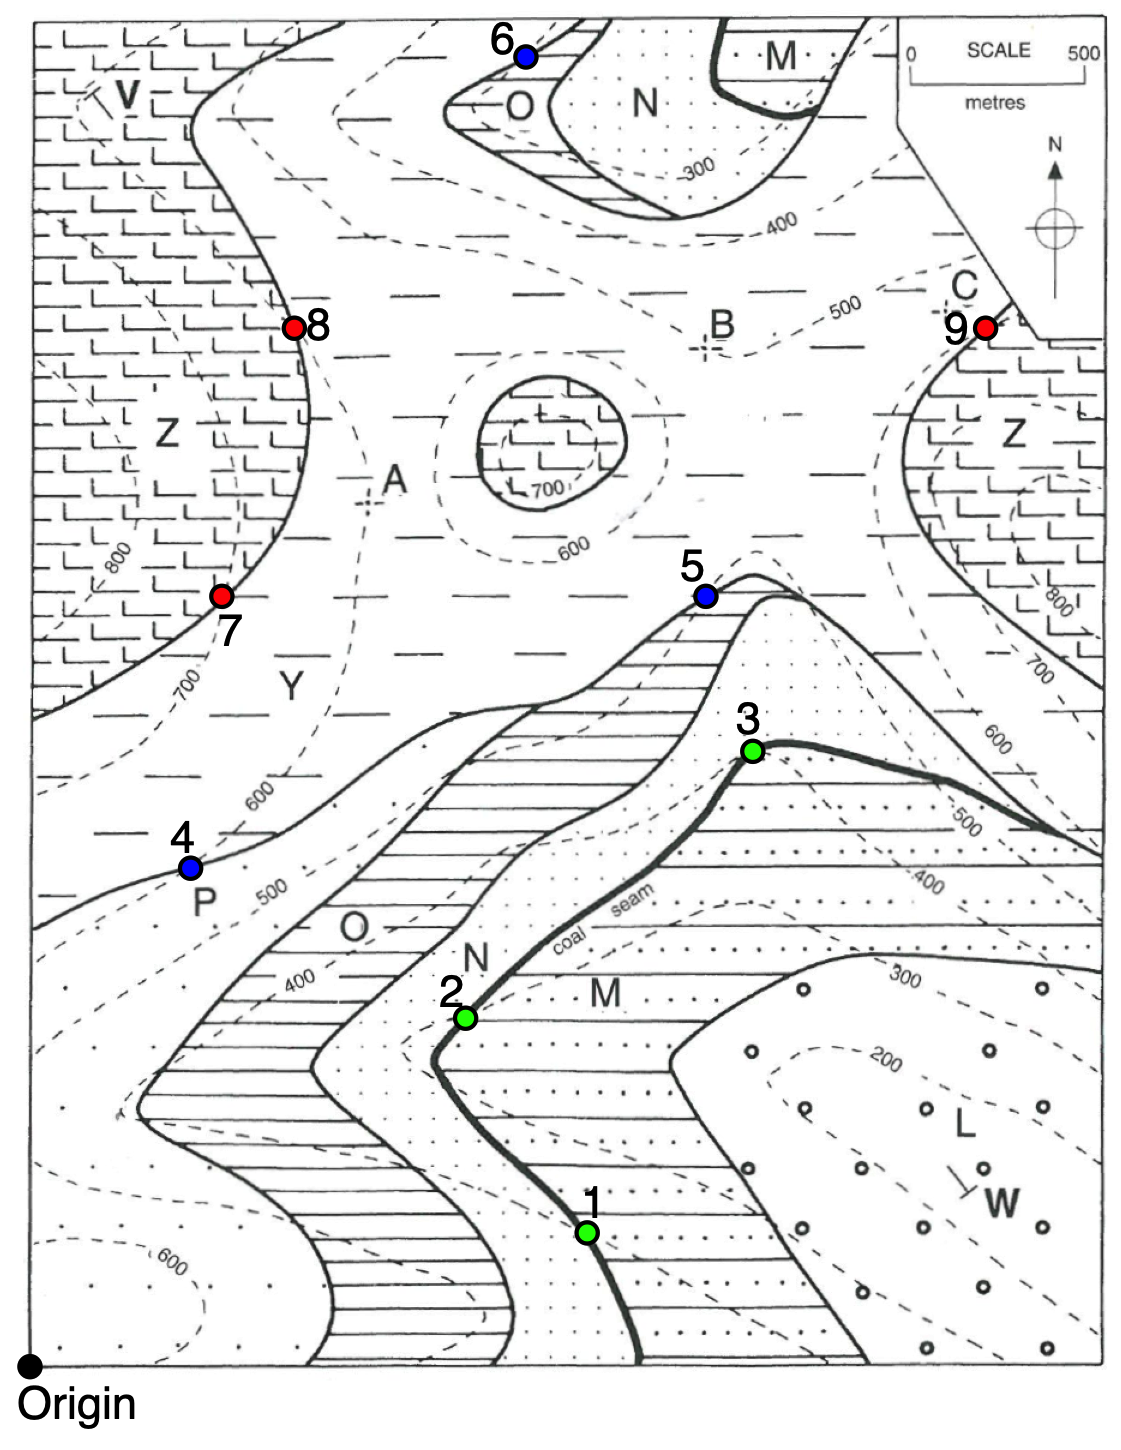
\includegraphics[width=9cm]{Figures/ch4f8.png}
    \caption{Map for exercise 4. This is map 10 of Bennison et al. (2011).}
    \end{figure}
    
    point1 = [1580, 379, 400]
    
    point2 = [1234, 992, 300]
    
    point3 = [2054, 1753, 400]
    
    point4 = [448, 1424, 600]
    
    point5 = [1921, 2195, 500]
    
    point6 = [1408, 3737, 300]
    
    point7 = [536, 2196, 700]
    
    point8 = [743, 2963, 600]
    
    point9 = [2720, 2963, 600]
    
    \begin{enumerate}
        \item Compute the strike and dip of the coal seam (points 1-3).
        \item Compute the strike and dip of the contact where the blue points 4-6 are located. What kind of contact is this? Is the coal seam below or above this contact?
        \item Compute the strike and dip of the contact between units Y and Z (points 7-9). Is this contact below or above the contact in b?
        \item The line of section V-W has a trend of 142\degree. What is the apparent dip of the three contacts above along the section?
        \item Draw a schematic cross section along line V-W
    \end{enumerate}
    
    \textit{Hint}: Use function \textit{ThreePoint} to solve a, b and c. Use function \textit{Angles} to solve d.
    
    \item The map of Fig. 4.8 shows an area of a reconnaissance survey in the Appalachian Valley and Ridge Province of western Maryland, USA. On the western half of the map, the contact between a shale horizon (B) and a sandstone unit (C) has been located in two areas. Three points on this contact have the following \textbf{ENU} coordinates:
    
     \begin{figure}[ht]
    \centering
    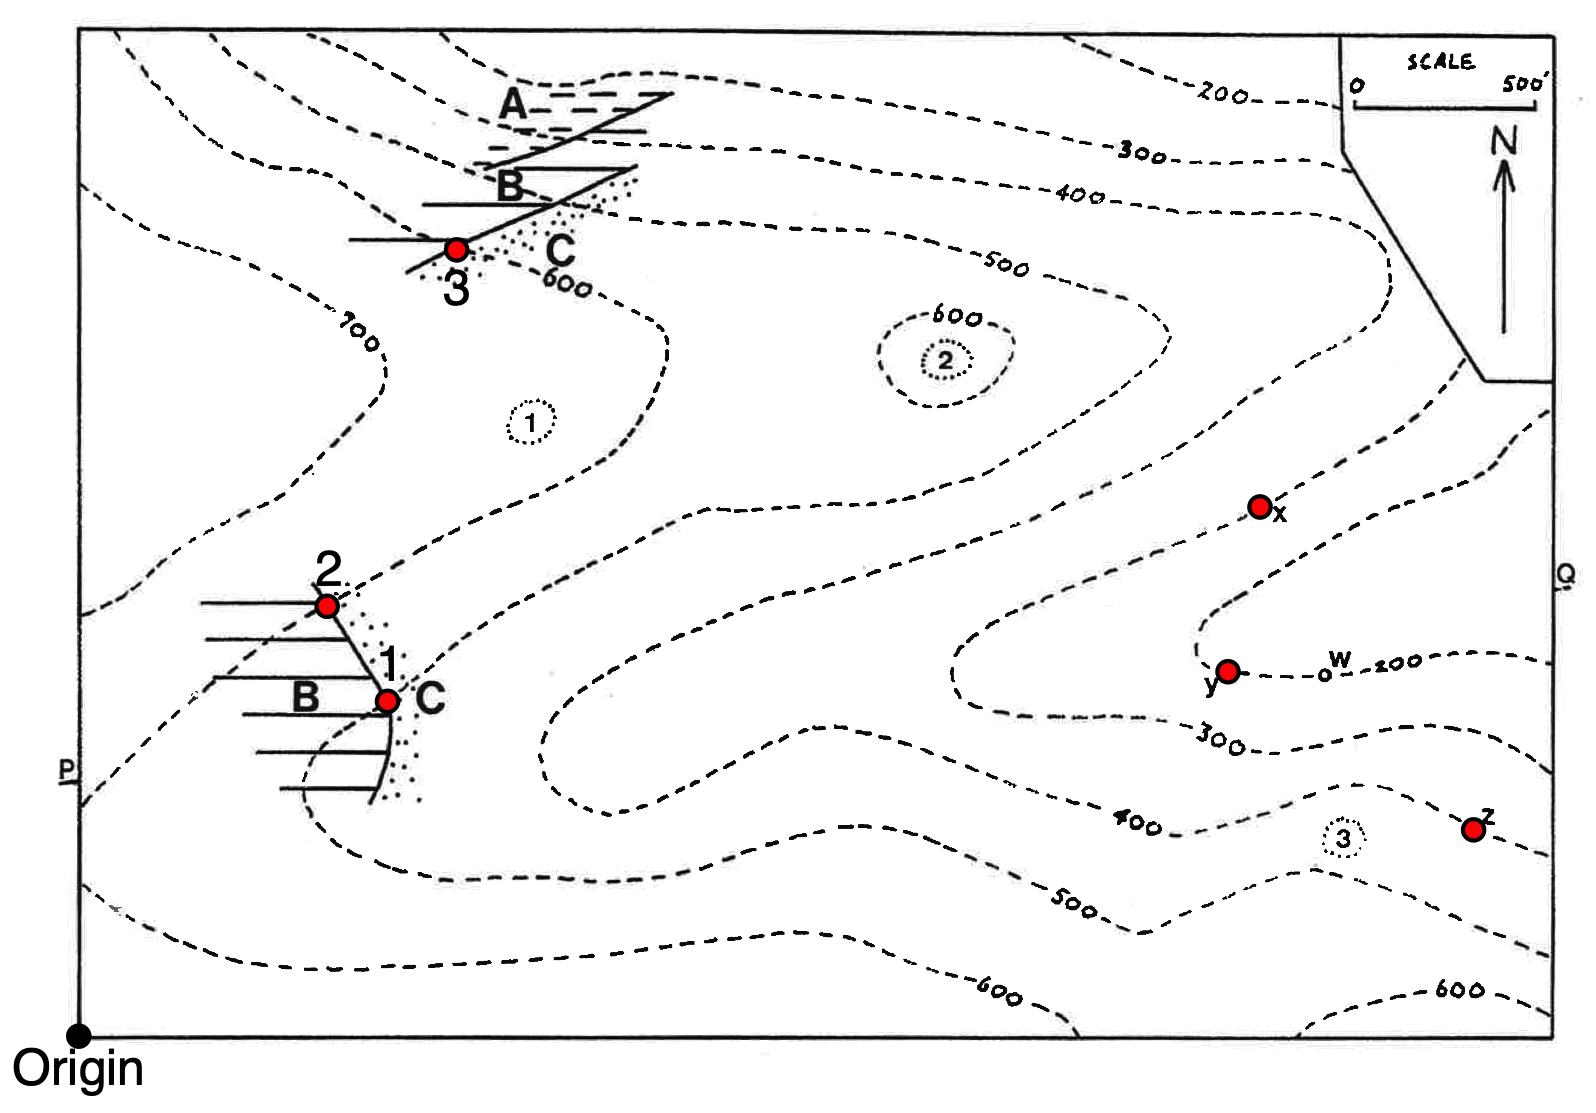
\includegraphics[width=12cm]{Figures/ch4f9.png}
    \caption{Map for exercise 5}
    \end{figure}
    
    point1 = [862, 943, 500]
    
    point2 = [692, 1212, 600]
    
    point3 = [1050, 2205, 600]
    
    On the eastern half of the map, the contact between B and C was found exposed at three locations labelled x, y, and z. The \textbf{ENU} coordinates of these points are:
    
    pointx = [3298, 1487, 300]
    
    pointy = [3203, 1031, 200]
    
    pointz = [3894, 590, 400]
    
    \begin{enumerate}
        \item Compute the strike and dip of the contact on the western half of the map.
        \item Compute the strike and dip of the contact on the eastern half of the map.
        \item What kind of structure is present on the map? 
        \item Compute the intersection of the western and eastern contacts. What does this line represent?
    \end{enumerate}
    
     \textit{Hint}: Use function \textit{ThreePoint} to solve a and b. Use function \textit{Angles} to solve d.
     
     \item In problem 3, the error in azimuth is 5\degree and in apparent dip is 3\degree. What is the uncertainty in the true dip of the bed? \textit{Hint}: Use function \textit{AnglesU}.
     
     \item In the map of Fig. 4.7, the east and north coordinates of the points have 15 m error, and the elevations have 5 m error. 
     \begin{enumerate}
        \item What is the uncertainty in the strike and dip of the coal seam?
        \item What is the uncertainty in the strike and dip of the unconformity?
        \item What is the angle between the unconformity and the coal seam and what is the uncertainty in this angle?
    \end{enumerate}
    \textit{Hint}: Use functions \textit{ThreePointU} and \textit{AnglesU}.

\end{enumerate}

\addcontentsline{toc}{section}{References}
\section*{References}

Allmendinger, R.W., Cardozo, N. and Fisher, D.W. 2012. Structural Geology Algorithms: Vectors and Tensors. Cambridge University Press, 302 p.

Bennison, G.M., Olver, P.A. and Moseley, K.A. 2011. An Introduction to Geological Structures and Maps, 8th edition. Hodder Education, 168 p.

Fisher, N.I., Lewis, T. and Embleton, B.J.J. 1987. Statistical analysis of spherical data. Cambridge University Press, 329 p.

Leyshon, P.R. and Lisle, R.J. 1996. Stereographic Projection Techniques in Structural Geology. Butterworth Heinemann, 104 p.

Marshak, S. and Mitra, G. 1988. Basic Methods of Structural Geology. Prentice Hall, 446 p.

Ragan, D.M. 2009. Structural Geology: An Introduction to Geometrical Techniques. Cambridge University Press, 632 p.

Taylor, J.R. 1997. An Introduction to Error Analysis, 2nd edition. University Science Books, 327 p.

% CHAPTER 5: 
\chapter{Transformations}

Many problems in geology become simpler when viewed from another perspective. For example, when studying the movement of continents through time because of plate tectonics (Fig. 5.1a), two coordinate systems are required, one in a present-day geographic frame, and another one attached to the continent. Or to analyze a fault (Fig. 5.1b), we need one coordinate system attached to the fault (with one axis parallel to the pole and another to the slickensides), which we want to relate to the more familiar \textbf{NED} system. A change in coordinate system is called a coordinate transformation and this is an operation that happens everytime and everywhere. Computer games, flight simulators, and 3D interpretation programs rely heavily on coordinate transformations. 

 \begin{figure}[ht]
    \centering
    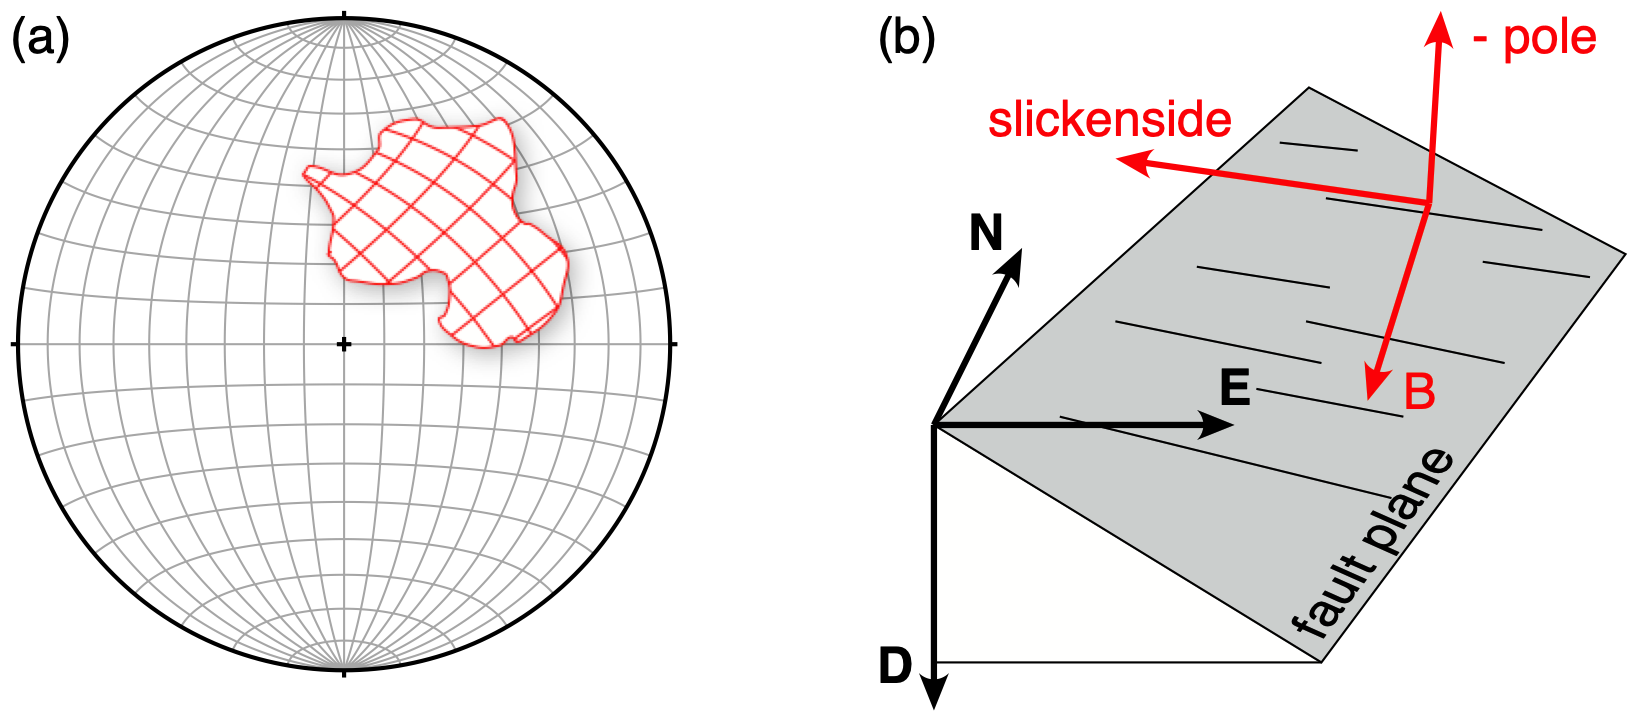
\includegraphics[width=12cm]{Figures/ch5f1.png}
    \caption{Examples of coordinate transformations in geology. \textbf{a.} Continental drift, \textbf{b.} A fault plane. Red is the coordinate system for analysis, and gray is the geographic coordinate system. Modified from Allmendinger et al. (2012).}
\end{figure}

\section{Transforming coordinates and vectors}

\subsection{Coordinate transformations}

A transformation involves a change in the origin and orientation of the coordinate system. We will refer to the new axes as the primed coordinate system, $\mathbf{X\text{$'$}}$, and the old coordinate system as the unprimed system, $\mathbf{X}$ (Fig. 5.2a). Let's assume the origin of the old and new coordinate systems is the same. The change in orientation of the new coordinate system is defined by the angles between the new coordinate axes and the old axes. These angles are marked systematically, the first subscript refers to the new coordinate axis and the second subscript to the old coordinate axis. For example, $\theta_{23}$ is the angle between the $\mathbf{X_2\text{$'$}}$ axis and the $\mathbf{X_3}$ axis (Fig. 5.2a). 

 \begin{figure}[H]
    \centering
    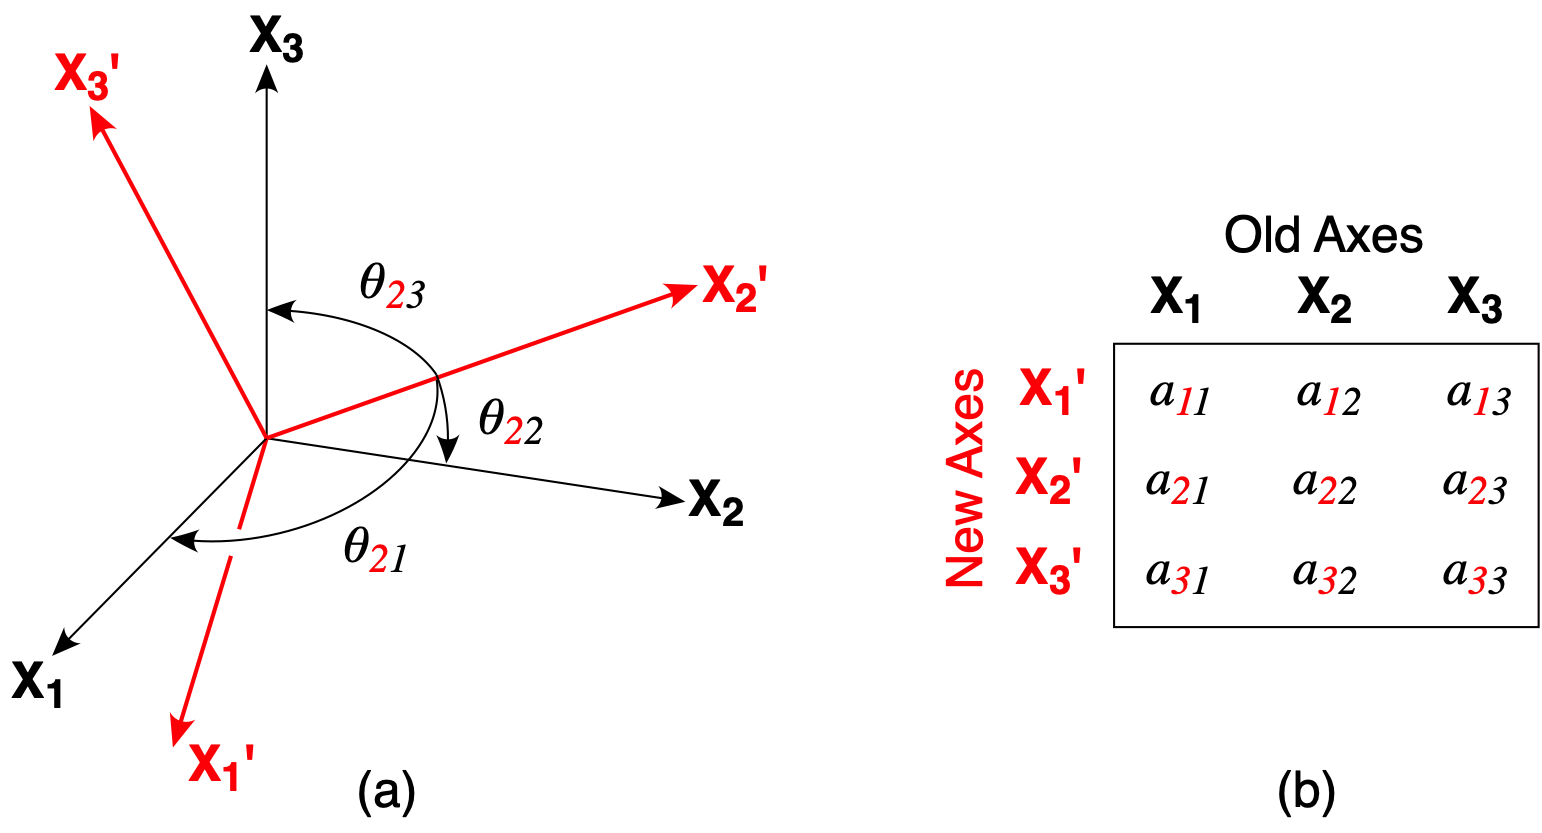
\includegraphics[width=12cm]{Figures/ch5f2.png}
    \caption{\textbf{a.} Rotation of a Cartesian coordinate system. The old axes are black, the new axes are primed and red. Only three of the nine possible angles are shown. \textbf{b.} Graphic device for remembering how the subscript of the direction cosines relate to the new and the old axes. Modified from Allmendinger et al. (2012).}
\end{figure}

To define the transformation, we use the cosines of these angles rather than the angles themselves (Fig. 5.2b). These are the direction cosines of the new axes with respect to the old axes. The subscript convention is exactly the same. For example, $a_{23}$ is the direction cosine of the $\mathbf{X_2\text{$'$}}$ axis with respect to the $\mathbf{X_3}$ axis. There are nine direction cosines that form a 3 $\times$ 3 array, where each row refers to a new axis and each column to an old axis (Fig. 5.2b). This matrix \textbf{a} of direction cosines is known as the \textit{transformation matrix}, and it is the key element that defines the transformation.

Fortunately, not all the nine direction cosines in the transformation matrix are independent. Since the base vectors of the new coordinate system are unit vectors, their magnitude is 1:

\begin{equation}
    \begin{split}
        a_{11}^2+a_{12}^2+a_{13}^2=1 \\
        a_{21}^2+a_{22}^2+a_{23}^2=1 \\
        a_{31}^2+a_{32}^2+a_{33}^2=1
    \end{split}
\end{equation}

and because the base vectors of the new coordinate system are perpendicular to each other, the dot product of two of these axes is zero:

\begin{equation}
    \begin{split}
        a_{21}a_{31}+a_{22}a_{32}+a_{23}a_{33}=0 \\
        a_{31}a_{11}+a_{32}a_{12}+a_{33}a_{13}=0 \\
        a_{11}a_{21}+a_{12}a_{22}+a_{13}a_{23}=0
    \end{split}
\end{equation}

Equations 5.1 and 5.2 are known as the \textit{orthogonality relations}. Since we have nine unknowns (i.e. the nine direction cosines) and six equations, there are only three independent direction cosines in the transformation matrix. If we know three of the direction cosines defining the transformation, we can calculate the other six.

\subsection{Transformation of vectors}

Once we know the transformation matrix \textbf{a} and the components of a vector in the old coordinate system, we can calculate the components of the vector in the new coordinate system. The equations are fairly simple:

\begin{equation}
    \begin{split}
        v_1\text{$'$}=a_{11}v_1+a_{12}v_2+a_{13}v_3 \\
        v_2\text{$'$}=a_{21}v_1+a_{22}v_2+a_{23}v_3 \\
        v_3\text{$'$}=a_{31}v_1+a_{32}v_2+a_{33}v_3
    \end{split}
\end{equation}

or using the Einstein summation notation:

\begin{equation}
    v_i\text{$'$}=a_{ij}v_j
\end{equation}

where \textit{i} is the free suffix, and \textit{j} is the dummy suffix. Assuming that ($i,\,j=1,2,3$), Equation 5.4 represents three separate equations (the three indexes of \textit{i}), each one with three terms (the three indexes of \textit{j}). These equations are easy to implement in Python code:

\begin{center}
\begin{lstlisting}[language=Python, frame=single]
for i in range(0,3,1):
    v_new[i] = 0
    for j in range(0,3,1):
        v_new[i] = a[i,j]*v_old[j] + v_new[i]
\end{lstlisting}
\end{center}

You will see this code snippet repeatedly in the functions of this chapter. Linear algebra is very elegant. To convert the vector from the new coordinate system back to the old coordinate system, you just need to do:

\begin{equation}
    v_i=a_{ji}v_j\text{$'$}
\end{equation}

or in Python code:

\begin{center}
\begin{lstlisting}[language=Python, frame=single]
for i in range(0,3,1):
    v_old[i] = 0
    for j in range(0,3,1):
        v_old[i] = a[j,i]*v_new[j] + v_old[i]
\end{lstlisting}
\end{center}

\subsection{A simple transformation: From \textbf{ENU} to \textbf{NED}}

There is a simple coordinate transformation that nicely illustrates the theory above: the transformation from an \textbf{ENU} to a \textbf{NED} coordinate system (Fig. 4.1). It is simple because the angles involved are either 0, 90, or 180\degree. The direction cosines of the new axes (\textbf{NED}) with respect to the old axes (\textbf{ENU}), and the transformation matrix \textbf{a} is:

\begin{equation}
    \textbf{a}=
    \begin{bmatrix}
    \cos{90} & \cos{0} & \cos{90} \\
    \cos{0} & \cos{90} & \cos{90} \\
    \cos{90} & \cos{90} & \cos{180}
\end{bmatrix}
\end{equation}

which simplifies to:

\begin{equation}
    \textbf{a}=
    \begin{bmatrix}
    0 & 1 & 0 \\
    1 & 0 & 0 \\
    0 & 0 & -1
\end{bmatrix}
\end{equation}

When we use this matrix in Eq. 5.4, we get:

\begin{equation}
    v_1\text{$'$}=v_2;\quad v_2\text{$'$}=v_1; \quad v_3\text{$'$}=-v_3;
\end{equation}

Notice that in this special case \textbf{a} is symmetric ($a_{ij}=a_{ji}$), so the elements of \textbf{a} are also the direction cosines of  \textbf{ENU} with respect to \textbf{NED}. In the following sections, we will look at more complicated coordinate transformations, but the principles mentioned here will still apply.

\section{Applications}

\subsection{Stratigraphic thickness}

The thickness of a stratigraphic unit is the perpendicular distance between the parallel planes bounding the unit. This is also called the true or stratigraphic thickness (Ragan, 2009). A general problem though is that points on the planes bounding the unit, are commonly given in a geographic (e.g. \textbf{ENU}) coordinate system. One therefore must use ortographic projections and trigonometry to determine the stratigraphic thickness of the unit from the points (Ragan, 2009).

An easier approach is to use a transformation. Figure 5.3 illustrates the situation. Points on the top and base of the unit are given in an \textbf{ENU} coordinate system. We can transform these points into a coordinate system attached to the bounding planes, where the strike (RHR) of the planes is the first axis, the dip the second axis, and the pole to the planes the third axis. We will call this coordinate system the \textbf{SDP} system. The thickness of the unit is just the difference between the \textbf{P} coordinate of a point on the top of the unit and the \textbf{P} coordinate of any point on the base.

 \begin{figure}[H]
    \centering
    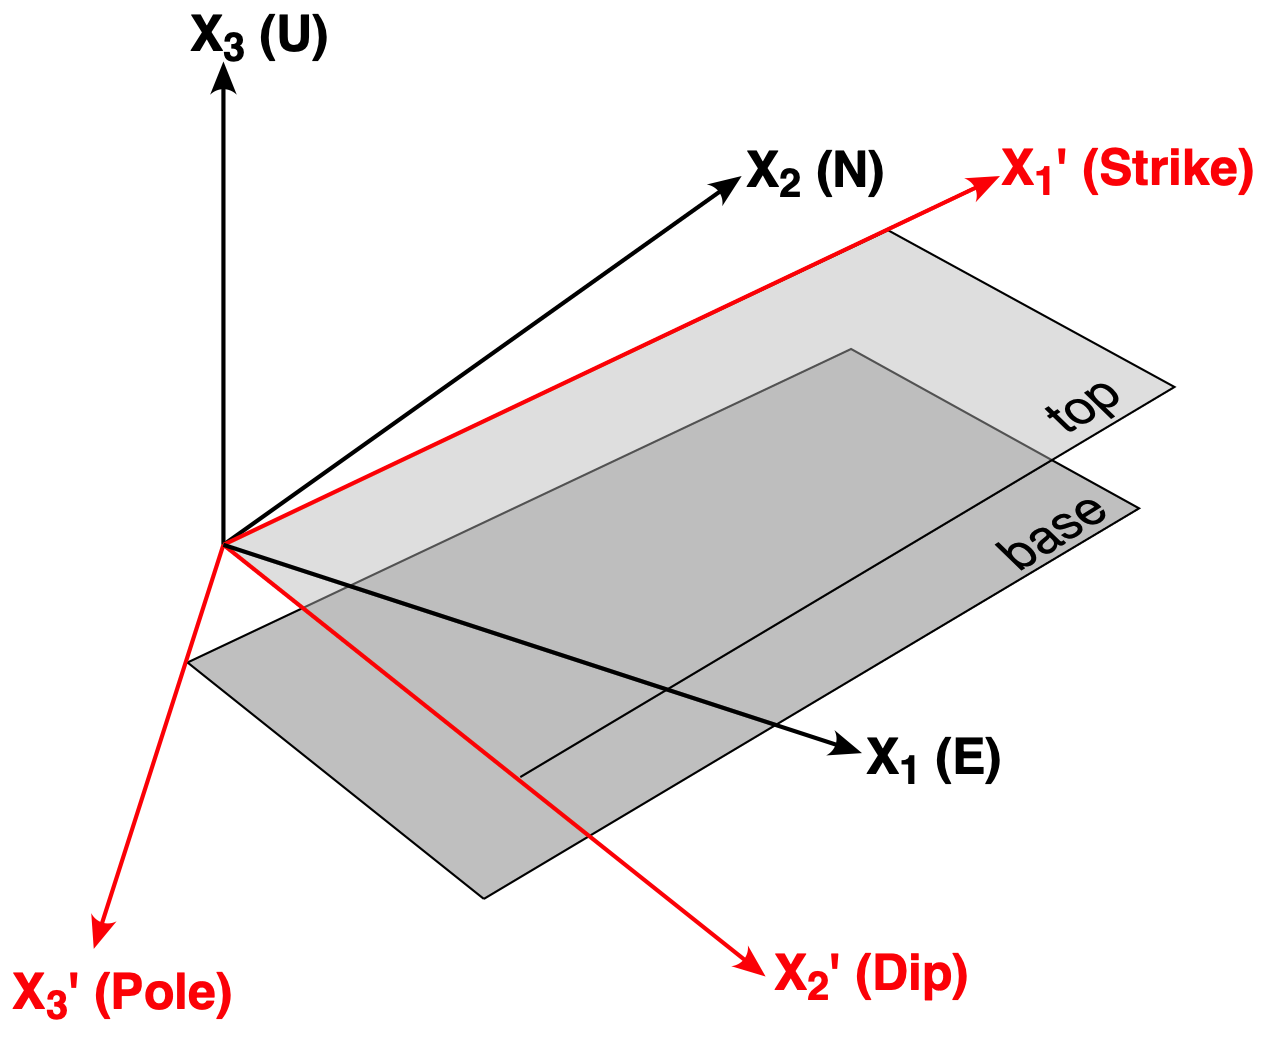
\includegraphics[width=10cm]{Figures/ch5f3.png}
    \caption{Coordinate transformation from an \textbf{ENU} to a Strike-Dip-Pole (\textbf{SDP}) coordinate system. The thickness of the unit can be calculated by subtracting the \textbf{P} coordinates of any point on the top and any point on the base. Modified from Allmendinger (2019).}
\end{figure}

We can find the elements of the matrix \textbf{a} for this transformation using trigonometry. However, we will follow a more didactic approach. We will reference the two \textbf{ENU} and \textbf{SDP} coordinate systems with respect to the \textbf{NED} coordinate system, and use the dot product to determine the direction cosines of \textbf{SDP} into \textbf{ENU}. 

The direction cosines of the \textbf{ENU} coordinate system with respect to the \textbf{NED} coordinate system are given by Eq. 5.7. The direction cosines of the \textbf{SDP} coordinate system with respect to the \textbf{NED} coordinate system are given by Table \ref{table4.1}:

\begin{gather*}
    \mathbf{S} = [\cos(strike),\sin(strike),0] \\
    \mathbf{D} = [\cos(strike+90)\cos(dip),\sin(strike+90)\cos(dip),\sin(dip)] \\
    \mathbf{P} = [\cos(strike-90)\cos(90-dip),\sin(strike-90)\cos(90-dip),\sin(90-dip)]
\end{gather*}

which simplifies to:

\begin{equation}
    \begin{split}
        \mathbf{S} = [\cos(strike),\sin(strike),0] \hspace{70pt}  \\
        \mathbf{D} = [-\sin(strike)\cos(dip),\cos(strike)\cos(dip),\sin(dip)] \\
        \mathbf{P} = [\sin(strike)\sin(dip),-\cos(strike)\sin(dip),\cos(dip)]
    \end{split}
\end{equation}

The transformation matrix \textbf{a} from the \textbf{ENU} to the \textbf{SDP} coordinate system has as components the direction cosines of the new \textbf{SDP} axes into the old \textbf{ENU} axes. From Eq. 4.9, one can see that these are just the dot product between the new and old axes:

\begin{equation*}
    \textbf{a}=
    \begin{bmatrix}
    \mathbf{S}\cdot\mathbf{E} & \mathbf{S}\cdot\mathbf{N} & \mathbf{S}\cdot\mathbf{U} \\
    \mathbf{D}\cdot\mathbf{E} & \mathbf{D}\cdot\mathbf{N} & \mathbf{D}\cdot\mathbf{U} \\
    \mathbf{P}\cdot\mathbf{E} & \mathbf{P}\cdot\mathbf{N} & \mathbf{P}\cdot\mathbf{U}
\end{bmatrix}
\end{equation*}

which is equal to:

\begin{equation}
    \textbf{a}=
    \begin{bmatrix}
    \sin(strike) & \cos(strike & 0 \\
    \cos(strike)\cos(dip) & -\sin(strike)\cos(dip) & -\sin(dip) \\
    -\cos(strike)\sin(dip) & \sin(strike)\sin(dip) & -\cos(dip)
\end{bmatrix}
\end{equation}

So if point 1 is at the top of the unit and has coordinates $[E_1,N_1,U_1]$, and point 2 is at the base of the unit and has coordinates $[E_2,N_2,U_2]$, the \textbf{P} coordinates of these points are:

\begin{equation}
    \begin{split}
        P_1 = -\cos(strike)\sin(dip)E_1+\sin(strike)\sin(dip)N_1-\cos(dip)U_1  \\
        P_2 = -\cos(strike)\sin(dip)E_2+\sin(strike)\sin(dip)N_2-\cos(dip)U_2  \\
    \end{split}
\end{equation}

and the thickness of the unit is:

\begin{equation}
    t = P_2-P_1
\end{equation}{}

The function \href{https://github.com/nfcd/compGeo/blob/master/source/functions/TrueThickness.py}{\textit{TrueThickness}} calculates the thickness of a unit given the strike and dip of the unit, and the \textbf{ENU} coordinates of two points at the top and base of the unit:

\begin{lstlisting}[language=Python, frame=single]
import numpy as np

def TrueThickness(strike,dip,top,base):
    '''
    TrueThickness calculates the thickness (t) of a unit 
    given the strike (strike) and dip (dip) of the unit, 
    and points at its top (top) and base (base) 

    top and base are 1 x 3 arrays defining the location 
    of top and base points in an ENU coordinate system. 
    For each one of these arrays, the first, second
    and third entries are the E, N and U coordinates

    NOTE: strike and dip should be input in radians
    '''
    # make the transformation matrix from ENU coordinates 
    # to SDP coordinates. Eq. 5.10
    sinStr = np.sin(strike)
    cosStr = np.cos(strike)
    sinDip = np.sin(dip)
    cosDip = np.cos(dip)
    a = np.array([[sinStr, cosStr, 0],
    [cosStr*cosDip, -sinStr*cosDip, -sinDip],
    [-cosStr*sinDip, sinStr*sinDip, -cosDip]])
    
    # transform the top and base points 
    # from ENU to SDP coordinates. Eq. 5.4 
    topn = np.zeros(3)
    basen = np.zeros(3)
    for i in range(0,3,1):
        for j in range(0,3,1):
            topn[i] = a[i,j]*top[j] + topn[i]
            basen[i] = a[i,j]*base[j] + basen[i]
    
    # compute the thickness of the unit. Eq. 5.12
    t = np.abs(basen[2] - topn[2])
    
    return t
\end{lstlisting}
 
Let's use this function to determine the thickness of the sedimentary units T to Q in the geologic map of Fig. 5.4. This time we have points at the top and base of these units, and their \textbf{ENU} coordinates are:

 \begin{figure}[H]
    \centering
    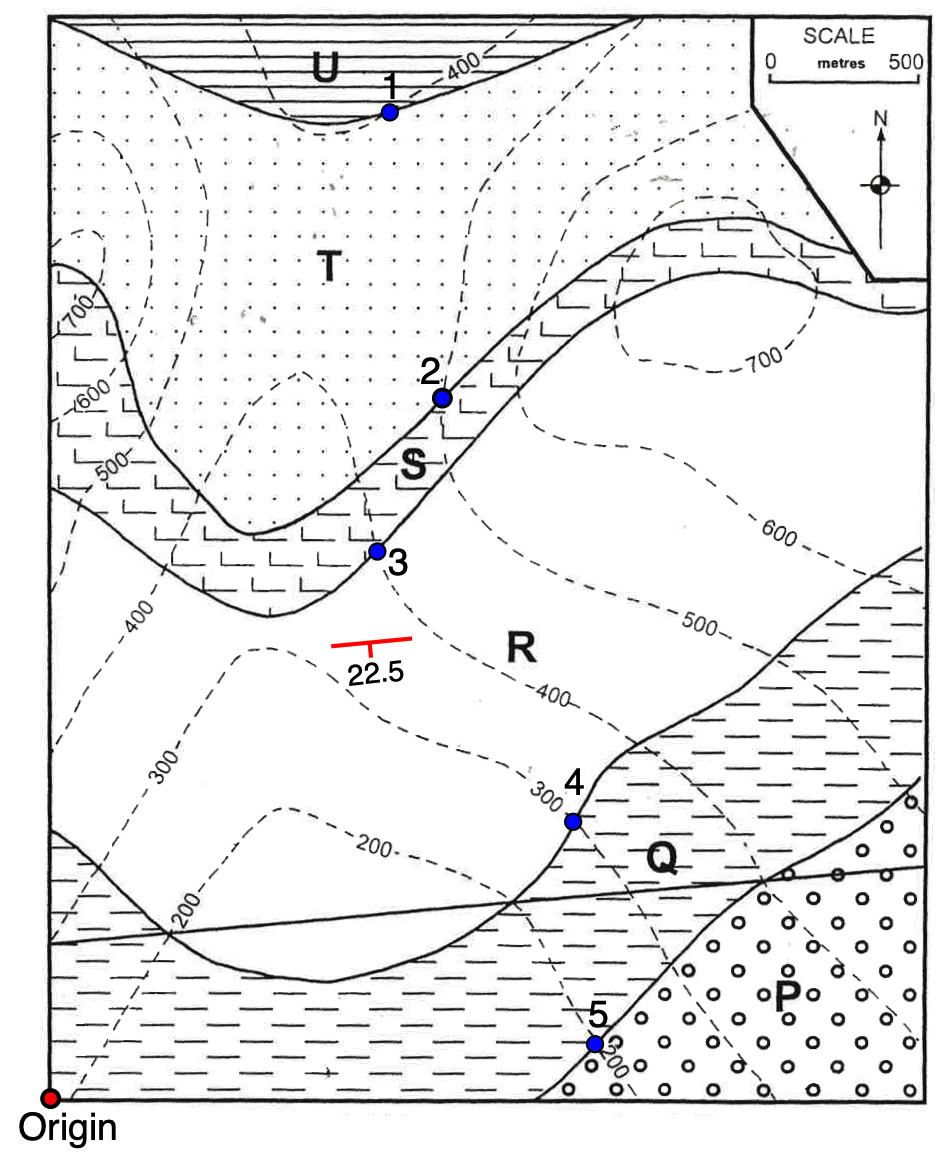
\includegraphics[width=9cm]{Figures/ch5f4.png}
    \caption{Geologic map of sedimentary units with an orientation 84.5/22.5 (RHR) (Bennison et al.,  2011). Points at the top and base of units T to Q are used to determine the thickness of the units.}
\end{figure}

point1 = [1147, 3329, 400]

point2 = [1323, 2362, 500]

point3 = [1105, 1850, 400]

point4 = [1768, 940, 300]

point5 = [1842, 191, 200]

The Python notebook \href{https://github.com/nfcd/compGeo/blob/master/source/notebooks/ch5-1.ipynb}{ch5-1} shows the solution to this problem:

\begin{center}
\begin{lstlisting}[language=Python, frame=single]
import numpy as np
pi = np.pi

import sys
import os
sys.path.append(os.path.abspath('../functions'))
from TrueThickness import TrueThickness as TrueThickness

# Strike and dip of the unit in radians
strike = 84.5 * pi/180
dip = 22.5 * pi/180

# ENU coordinates of the points
p1 = np.array([1147, 3329, 400]) 
p2 = np.array([1323, 2362, 500]) 
p3 = np.array([1105, 1850, 400]) 
p4 = np.array([1768, 940, 300]) 
p5 = np.array([1842, 191, 200])

# Compute the thickness of the units
thickT = TrueThickness(strike,dip,p2,p1)
thickS = TrueThickness(strike,dip,p3,p2)
thickR = TrueThickness(strike,dip,p4,p3)
thickQ = TrueThickness(strike,dip,p5,p4)
print('Thickness of unit T = {:.1f} m'.format(thickT))
print('Thickness of unit S = {:.1f} m'.format(thickS))
print('Thickness of unit R = {:.1f} m'.format(thickR))
print('Thickness of unit Q = {:.1f} m'.format(thickQ))
\end{lstlisting}
\fbox{
    \parbox{\textwidth - 2 \fboxsep}{
    Output: \\
    Thickness of unit T = 467.2 m \\
    Thickness of unit S = 94.6 m \\
    Thickness of unit R = 278.6 m \\
    Thickness of unit Q = 195.6 m
}}
\end{center}

What about if there are uncertainties in the strike and dip of the unit, and in the top and base points? The function \href{https://github.com/nfcd/compGeo/blob/master/source/functions/TrueThicknessU.py}{\textit{TrueThicknessU}} in the resource git repository handles this case. Suppose that in the problem above, the uncertainties in strike and dip are 4\degree and 2\degree respectively, the uncertainty in east and north coordinates is 10 m, and in elevation is 5 m. The Python notebook \href{https://github.com/nfcd/compGeo/blob/master/source/notebooks/ch5-2.ipynb}{ch5-2} shows the solution to this problem:

\begin{center}
\begin{lstlisting}[language=Python, frame=single]
import numpy as np
pi = np.pi
import uncertainties as unc

import sys
import os
sys.path.append(os.path.abspath('../functions'))
from TrueThicknessU import TrueThicknessU as TrueThicknessU

# Strike and dip of the unit in radians
strike = 84.5 * pi/180
dip = 22.5 * pi/180

# Strike and dip errors in radians
ustrike = 4 * pi/180
udip = 2 * pi/180

# Create the strike and dip with uncertainties
strike = unc.ufloat(strike, ustrike) # strike +/- ustrike
dip = unc.ufloat(dip, udip) # dip +/- udip

# ENU coordinates of the points
# with uncertainties in E-N = 10, and U = 5
p1 = np.array([unc.ufloat(1147, 10), unc.ufloat(3329, 10), unc.ufloat(400, 5)]) 
p2 = np.array([unc.ufloat(1323, 10), unc.ufloat(2362, 10), unc.ufloat(500, 5)]) 
p3 = np.array([unc.ufloat(1105, 10), unc.ufloat(1850, 10),unc.ufloat(400, 5)]) 
p4 = np.array([unc.ufloat(1768, 10), unc.ufloat(940, 10), unc.ufloat(300, 5)]) 
p5 = np.array([unc.ufloat(1842, 10), unc.ufloat(191, 10), unc.ufloat(200, 5)])

# Compute the thickness of the units
thickT = TrueThicknessU(strike, dip, p2, p1)
thickS = TrueThicknessU(strike, dip, p3, p2)
thickR = TrueThicknessU(strike, dip, p4, p3)
thickQ = TrueThicknessU(strike, dip, p5, p4) 
print('Thickness of unit T = {:.1f} m'.format(thickT))
print('Thickness of unit S = {:.1f} m'.format(thickS))
print('Thickness of unit R = {:.1f} m'.format(thickR))
print('Thickness of unit Q = {:.1f} m'.format(thickQ))
\end{lstlisting}
\fbox{
    \parbox{\textwidth - 2 \fboxsep}{
    Output: \\
    Thickness of unit T = 467.2+/-31.5 m \\
    Thickness of unit S = 94.6+/-20.4 m \\
    Thickness of unit R = 278.6+/-37.0 m \\
    Thickness of unit Q = 195.6+/-27.0 m \\
}}
\end{center}

For the thinnest unit S, the uncertainty in thickness is as much as 20\% the thickness of this unit!

\subsection{Outcrop trace of a plane} \label{outcrop}

The \textbf{ENU} to \textbf{SDP} transformation is useful to solve another important problem, namely the outcrop trace of a plane on irregular terrain (Fig. \ref{fig:outrace}). If we know the orientation of the plane (strike and dip), the \textbf{ENU} coordinates of the location where the plane outcrops, and the topography of the terrain as a digital elevation model (DEM\footnote{A grid of regularly spaced points in east and north and with elevation information.}), we can determine the outcrop trace of the plane using computation. The solution is surprisingly simple, the plane outcrops wherever the \textbf{P} coordinate of the terrain is equal to the \textbf{P} coordinate of the plane's outcrop location.

Let's call the \textbf{P} coordinate of the plane's outcrop location $P_1$, and the \textbf{P} coordinate of a point in the DEM grid $P_{gp}$. The difference between these two is:

\begin{equation}
    D=P_1-P_{gp}
\end{equation}

At each point in the DEM grid, we can calculate and store this difference. The plane will outcrop wherever $D$ is zero. Therefore, to draw the outcrop trace, we just need to contour the $D$ value of zero on the grid. The function \href{https://github.com/nfcd/compGeo/blob/master/source/functions/OutcropTrace.py}{\textit{OutcropTrace}} computes the value of $D$ on a DEM grid of regularly spaced points defined by \textbf{E} ($\mathbf{XG}$), \textbf{N} ($\mathbf{YG}$) and \textbf{U} ($\mathbf{ZG}$) coordinates. Notice that these arrays must follow the format given by the NumPy \textit{meshgrid} function:

\begin{lstlisting}[language=Python, frame=single]
import numpy as np

def OutcropTrace(strike,dip,p1,XG,YG,ZG):
    '''
    OutcropTrace estimates the outcrop trace of a plane,
    given the strike (strike) and dip (dip) of the plane,
    the ENU coordinates of a point (p1) where the plane
    outcrops, and a DEM of the terrain as a regular grid
    of points with E (XG), N (YG) and U (ZG) coordinates.
    
    After using this function, to draw the outcrop trace 
    of the plane, you just need to draw the contour 0 on 
    the grid XG,YG,DG
    
    NOTE: strike and dip should be input in radians
          p1 must be an array
          XG and YG arrays should be constructed using 
          the Numpy function meshgrid
    '''
    
    # make the transformation matrix from ENU coordinates to 
    # SDP coordinates. We just need the third row of this matrix
    a = np.zeros((3,3))
    a[2,0] = -np.cos(strike)*np.sin(dip) 
    a[2,1] = np.sin(strike)*np.sin(dip) 
    a[2,2] = -np.cos(dip);
    
    # Initialize DG
    n, m = XG.shape
    DG = np.zeros((n,m))
    
    # Estimate the P coordinate of the outcrop point p1
    P1 = a[2,0]*p1[0] + a[2,1]*p1[1] + a[2,2]*p1[2]
    
    # Estimate the P coordinate at each point of the DEM
    # grid and subtract P1. Eq. 5.13
    for i in range(n):
        for j in range(m):
            DG[i,j] = P1 - (a[2,0]*XG[i,j] + a[2,1]*YG[i,j] + a[2,2]*ZG[i,j])
    
    return DG  
\end{lstlisting}

Let's apply this function to the map of Fig. 5.5. On the western half of this map, the contact between units B and C outcrops at point 2 and has an orientation 020/22 (RHR). On the eastern half of the map, the same contact outcrops at point y and has an orientation 160/22 (RHR). The notebook \href{https://github.com/nfcd/compGeo/blob/master/source/notebooks/ch5-3.ipynb}{ch5-3} draws the outcrop trace of the contact. Notice that the \textbf{ENU} coordinates of the points of the DEM grid are input from the text files \href{https://github.com/nfcd/compGeo/blob/master/source/data/ch5-3/XG.txt}{\textit{XG}}, \href{https://github.com/nfcd/compGeo/blob/master/source/data/ch5-3/YG.txt}{\textit{YG}}, and \href{https://github.com/nfcd/compGeo/blob/master/source/data/ch5-3/ZG.txt}{\textit{ZG}}.

 \begin{figure}[ht]
    \centering
    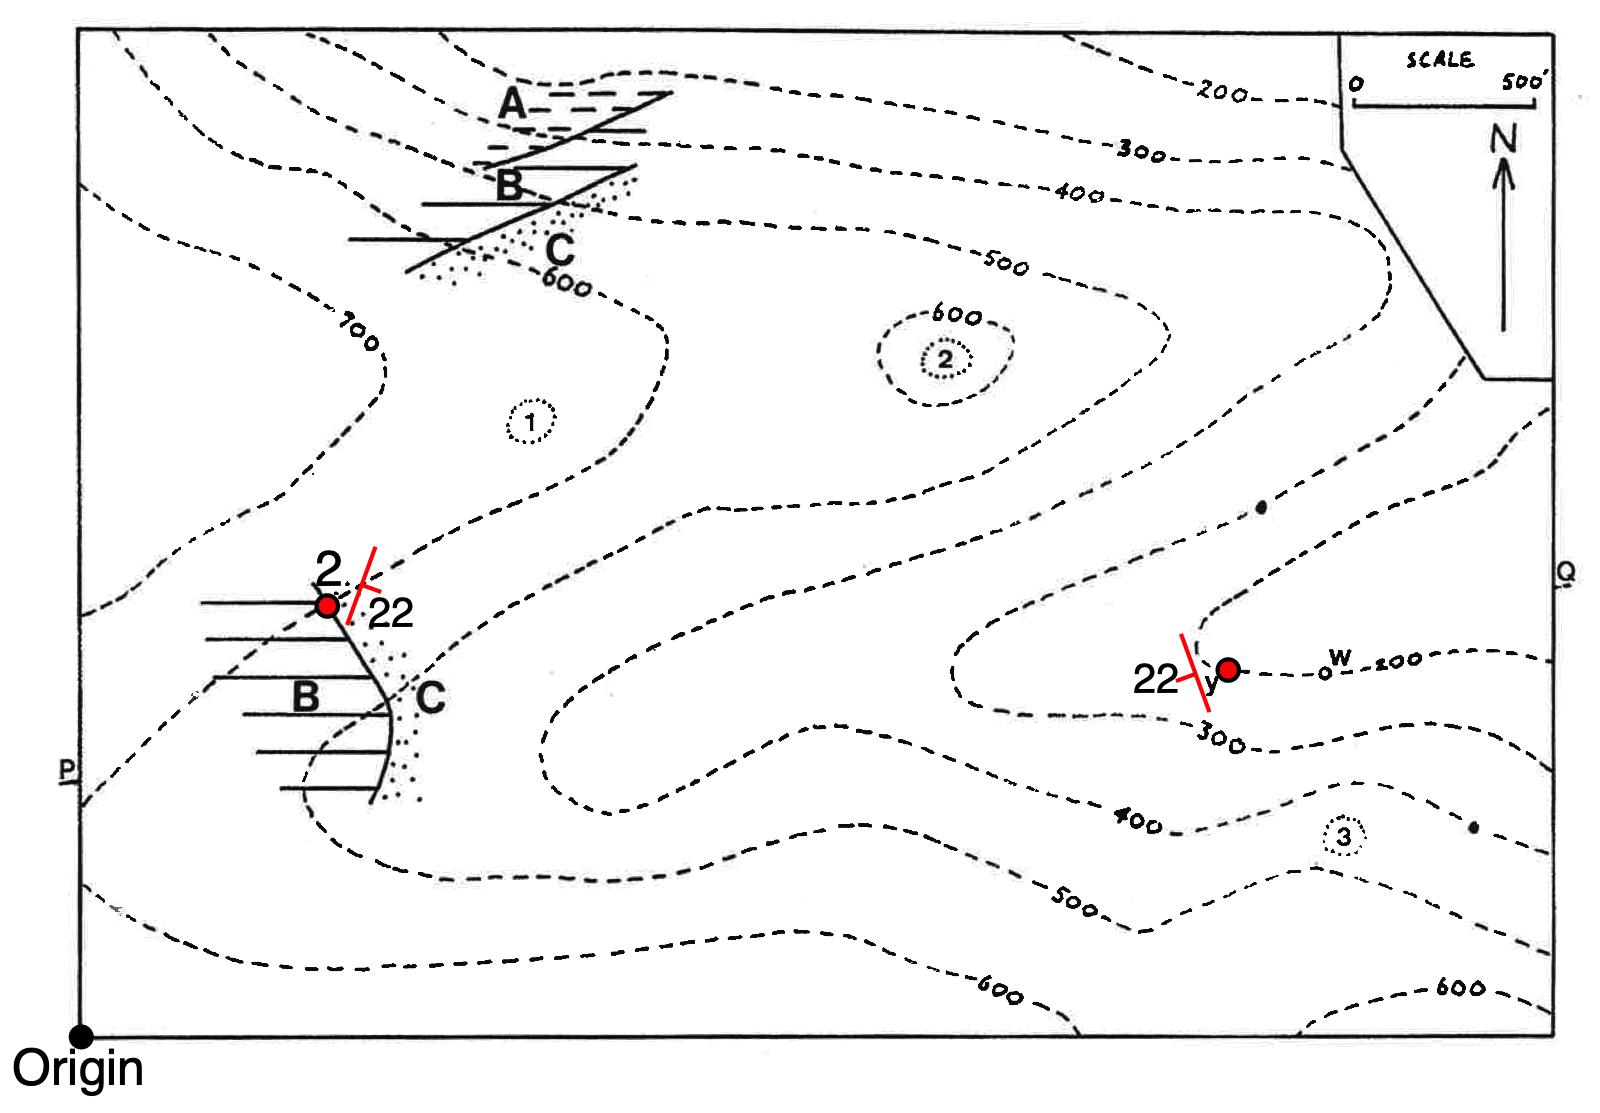
\includegraphics[width=11.8cm]{Figures/ch5f5.png}
    \caption{The contact between units B and C outcrops at point 2 with orientation 020/22 (RHR), and at point y with orientation 160/22 (RHR). From this information and a DEM of the terrain, we can determine the outcrop trace of the contact.}
\end{figure}

\begin{center}
\begin{lstlisting}[language=Python, frame=single]
import numpy as np
import matplotlib.pyplot as plt

import sys
import os
sys.path.append(os.path.abspath('../functions'))
from OutcropTrace import OutcropTrace as OutcropTrace

# Read the DEM grid
XG = np.loadtxt(os.path.abspath('../data/ch5-3/XG.txt'))
YG = np.loadtxt(os.path.abspath('../data/ch5-3/YG.txt'))
ZG = np.loadtxt(os.path.abspath('../data/ch5-3/ZG.txt'))

# Contour the terrain
cval = np.linspace(200,700,6)
cp = plt.contour(XG,YG,ZG,cval)
plt.clabel(cp, inline=True, fontsize=10, fmt="%d")

# Western contact
pi = np.pi
strike = 20*pi/180
dip = 22*pi/180
point2 = np.array([692, 1212, 600])
DG = OutcropTrace(strike,dip,point2,XG,YG,ZG)
cval = 0 # Contour only CG zero value
cp = plt.contour(XG,YG,DG,cval,colors='red',linewidths=3)

# Eastern contact
strike = 160*pi/180
dip = 22*pi/180
pointy = np.array([3203, 1031, 200])
DG = OutcropTrace(strike,dip,pointy,XG,YG,ZG)
cp = plt.contour(XG,YG,DG,cval,colors='red',linewidths=3)

# Make axes equal
plt.axis('scaled')
\end{lstlisting}
\fbox{
    \parbox{\textwidth - 2 \fboxsep}{
    Output: \\
    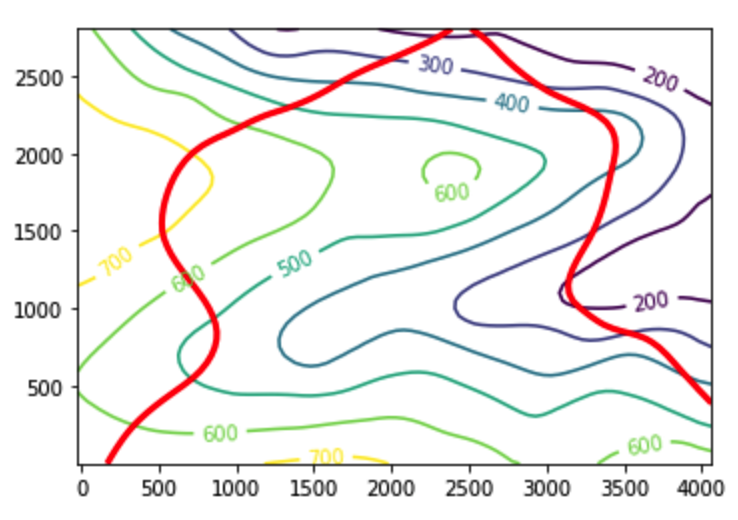
\includegraphics[width=9cm]{Figures/ch5f6.png}
}}
\end{center}

\subsection{Down-Plunge projection}

Folded rock layers normally have a cylindrical symmetry; the layers are bent about a single axis or direction, called the fold axis. The fold axis is a line of minimum, zero curvature, and the lines of maximum, non-zero curvature are perpendicular to it (Suppe, 1985). The least distorted view of such structure is in the plane perpendicular to the fold axis, which is called the profile plane (Fig. 5.7). Projecting the fold data to this profile plane is called a \textit{Down-Plunge} projection.

Constructing a Down-Plunge projection by hand typically involves an orthographic projection, and this problem is complicated (and tedious), particularly if points on the fold are not at the same elevation. Fortunately, we can solve this problem as a coordinate transformation, where points on the fold referenced in an \textbf{ENU} coordinate system, are transformed to a new $\mathbf{X_1\text{$'$}}\mathbf{X_2\text{$'$}}\mathbf{X_3\text{$'$}}$ coordinate system, with $\mathbf{X_3\text{$'$}}$ parallel to the fold axis, and $\mathbf{X_1\text{$'$}}\mathbf{X_2\text{$'$}}$ defining the profile plane (Fig. 5.6).

We will again derive the matrix \textbf{a} for this transformation using linear algebra. The direction cosines of the \textbf{ENU} coordinate system with respect to the \textbf{NED} coordinate system are given by Eq. 5.7. The direction cosines of the $\mathbf{X_1\text{$'$}}\mathbf{X_2\text{$'$}}\mathbf{X_3\text{$'$}}$ coordinate system with respect to the \textbf{NED} coordinate system are given by Table \ref{table4.1}. If the trend and plunge of the fold axis are $T$ and $P$, these direction cosines are (Fig. 5.6):

\begin{figure}[ht]
    \centering
    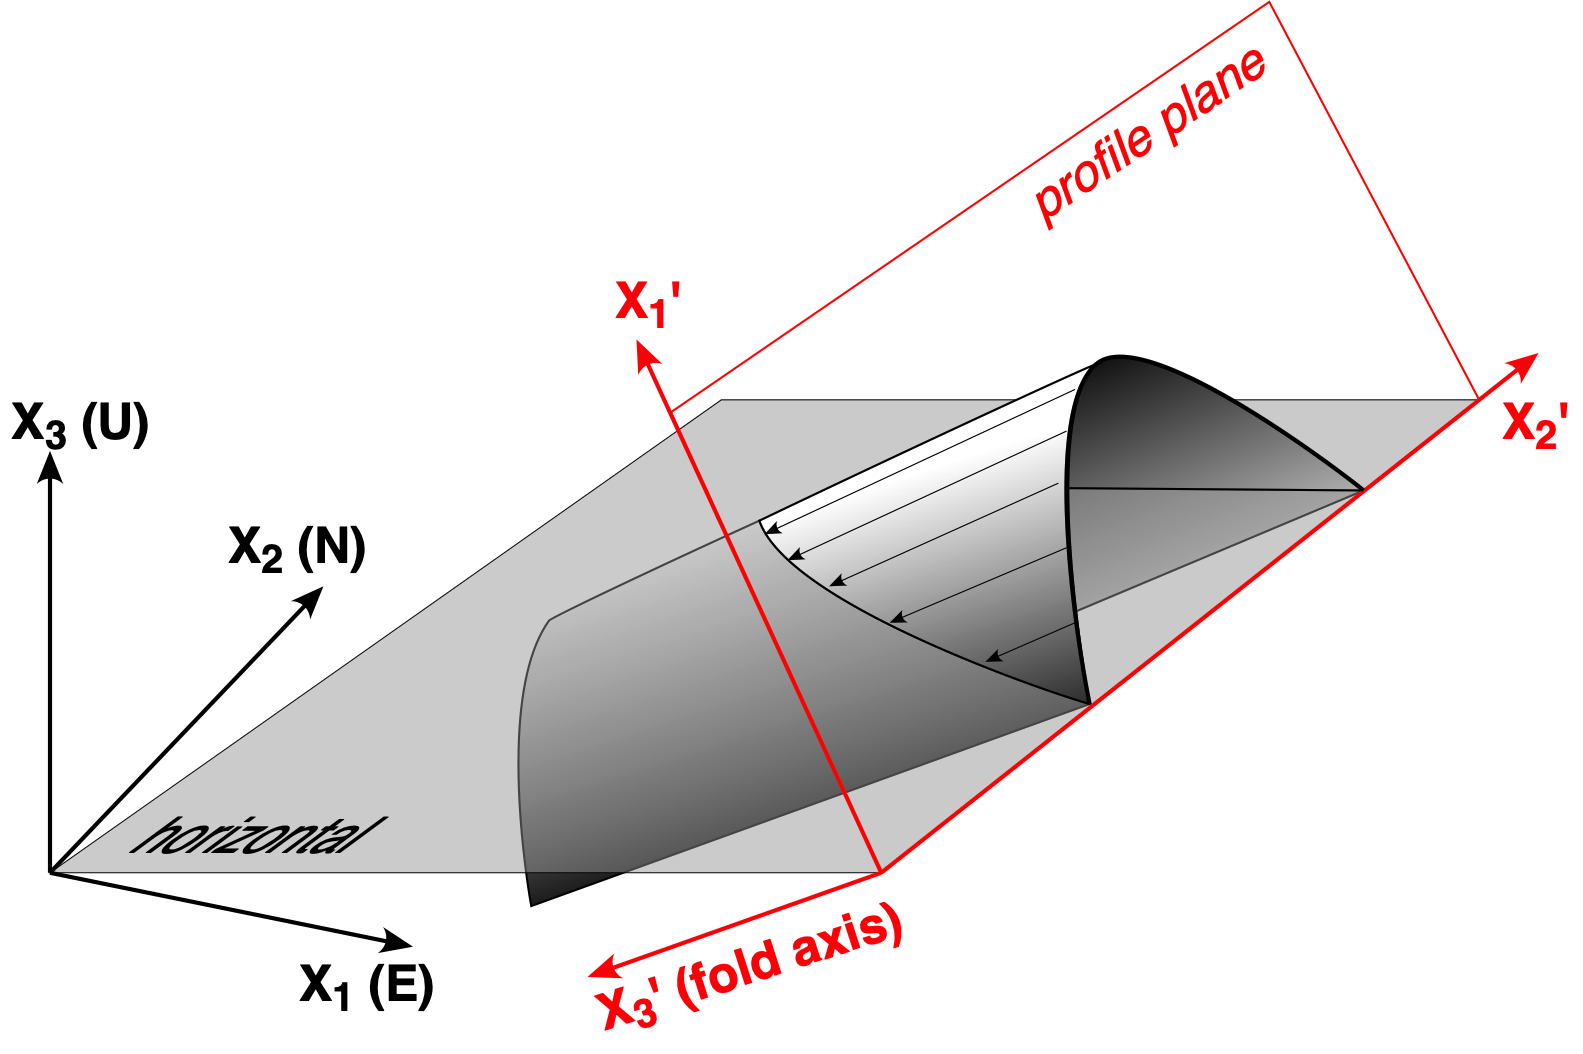
\includegraphics[width=12cm]{Figures/ch5f7.png}
    \caption{The two coordinate systems involved in a Down-Plunge projection of a fold. Modified from Allmendinger et al. (2012).}
\end{figure}

\begin{gather*}
    \mathbf{X_1\text{$'$}} = [\cos(T)\cos(P-90),\sin(T)\cos(P-90),\sin(P-90)] \\
    \mathbf{X_2\text{$'$}} = [\cos(T+90),\sin(T+90),0)] \\
    \mathbf{X_3\text{$'$}} = [\cos(T)\cos(P),\sin(T)\cos(P),\sin(P)]
\end{gather*}

which simplifies to:

\begin{equation}
    \begin{split}
        \mathbf{X_1\text{$'$}} = [\cos(T)\sin(P),\sin(T)\sin(P),-\cos(P)]  \\
        \mathbf{X_2\text{$'$}} = [-\sin(T),\cos(T),0] \hspace{40pt} \\
        \mathbf{X_3\text{$'$}} = [\cos(T)\cos(P),\sin(T)\cos(P),\sin(P)]
    \end{split}
\end{equation}

The direction cosines of the new $\mathbf{X_1\text{$'$}}\mathbf{X_2\text{$'$}}\mathbf{X_3\text{$'$}}$ axes into the old \textbf{ENU} axes are the dot product between the new and old axes:

\begin{equation*}
    \textbf{a}=
    \begin{bmatrix}
    \mathbf{X_1\text{$'$}}\cdot\mathbf{E} & \mathbf{X_1\text{$'$}}\cdot\mathbf{N} & \mathbf{X_1\text{$'$}}\cdot\mathbf{U} \\
    \mathbf{X_2\text{$'$}}\cdot\mathbf{E} & \mathbf{X_2\text{$'$}}\cdot\mathbf{N} & \mathbf{X_2\text{$'$}}\cdot\mathbf{U} \\
    \mathbf{X_3\text{$'$}}\cdot\mathbf{E} & \mathbf{X_3\text{$'$}}\cdot\mathbf{N} & \mathbf{X_3\text{$'$}}\cdot\mathbf{U}
\end{bmatrix}
\end{equation*}

which is equal to:

\begin{equation}
    \textbf{a}=
    \begin{bmatrix}
    \sin(T)\sin(P) & \cos(T)\sin(P) & \cos(P) \\
    \cos(T) & -\sin(T) & 0 \\
    \sin(T)\cos(P) & \cos(T)\cos(P) & -\sin(P)
\end{bmatrix}
\end{equation}

This is the transformation matrix \textbf{a} for the Down-Plunge projection. To project $i$ points on the fold with coordinates $[E_i,N_i,U_i]$, we just need to do the following:

\begin{equation}
    \begin{split}
        X_{1i}'=\sin(T)\sin(P)E_i+\cos(T)\sin(P)N_i+\cos(P)U_i \\
        X_{2i}'=\cos(T)E_i-\sin(T)N_i  \hspace{60pt}
    \end{split}
\end{equation}

and then plot $X_{2i}'$ against $X_{1i}'$ (Fig. 5.6) to draw the Down-Plunge projection of the fold.

The function \href{https://github.com/nfcd/compGeo/blob/master/source/functions/DownPlunge.py}{\textit{DownPlunge}} computes the Down-Plunge projection of a bed given the \textbf{ENU} coordinates of points on the bed, and the trend and plunge of the fold axis:

\begin{lstlisting}[language=Python, frame=single]
import numpy as np

def DownPlunge(bedseg,trd,plg):
   '''
   DownPlunge constructs the down plunge projection of a bed

   DownPlunge constructs the down plunge projection
   of a bed

   bedseg is a npoints x 3 array, which holds npoints 
   on the digitized bed, each point defined by
   3 coordinates: X1 = East, X2 = North, X3 = Up

   trd and plg are the trend and plunge of the fold axis

   NOTE: trd and plg should be entered in radians

   Python function translated from the Matlab function 
   DownPlunge in Allmendinger et al. (2012)
   '''
   # Number of points in bed
   nvtex = bedseg.shape[0]

   # Allocate some arrays
   a=np.zeros((3,3))
   dpbedseg = np.zeros((np.shape(bedseg)))
   
   # Calculate the transformation matrix a(i,j) Eq. 5.15
   a[0,0] = np.sin(trd)*np.sin(plg)
   a[0,1] = np.cos(trd)*np.sin(plg)
   a[0,2] = np.cos(plg)
   a[1,0] = np.cos(trd)
   a[1,1] = -np.sin(trd)
   a[2,0] = np.sin(trd)*np.cos(plg)
   a[2,1] = np.cos(trd)*np.cos(plg)
   a[2,2] = -np.sin(plg)
    
   # Perform transformation
   for nv in range(0,nvtex,1):
       for i in range(0,3,1):
           dpbedseg[nv,i] = 0.0
           for j in range(0,3,1):
               dpbedseg[nv,i] = a[i,j]*bedseg[nv,j] + dpbedseg[nv,i]
                
   return dpbedseg
\end{lstlisting}

Let's use this function to draw the Down-Plunge projection of the Big Elk anticline in southeastern Idaho, USA (Fig. 5.7; Albee and Cullins, 1975; Allmendinger et al., 2012). Text files contain the digitized contacts (\textbf{ENU}) of three tops along the fold: the Jurassic Twin Creek Limestone (\href{https://github.com/nfcd/compGeo/blob/master/source/data/ch5-4/jtc.txt}{\textit{jtc.txt}}), the Jurassic Stump Sandstone (\href{https://github.com/nfcd/compGeo/blob/master/source/data/ch5-4/js.txt}{\textit{js.txt}}), and the Cretaceous Peterson Limestone (\href{https://github.com/nfcd/compGeo/blob/master/source/data/ch5-4/kp.txt}{\textit{kp.txt}}). The trend and plunge of the folds axis is 125/126 (in the next chapter we will see how to compute this axis). The notebook \href{https://github.com/nfcd/compGeo/blob/master/source/notebooks/ch5-4.ipynb}{ch5-4} shows the solution to this problem:

\begin{lstlisting}[language=Python, frame=single]
import numpy as np
import matplotlib.pyplot as plt

import sys
import os
sys.path.append(os.path.abspath('../functions'))
from DownPlunge import DownPlunge as DownPlunge

# Trend and plunge of the fold axis in radians
trend = 125 * np.pi/180
plunge = 26 * np.pi/180

# Read the tops from the text files
jtc = np.loadtxt(os.path.abspath('../data/ch5-4/jtc.txt'))
js = np.loadtxt(os.path.abspath('../data/ch5-4/js.txt'))
kp = np.loadtxt(os.path.abspath('../data/ch5-4/kp.txt'))

# Transform the points
jtcdp = DownPlunge(jtc,trend,plunge)
jsdp = DownPlunge (js,trend,plunge)
kpdp = DownPlunge(kp,trend,plunge)

# Plot the down plunge section
plt.plot(jtcdp[:,1],jtcdp[:,0],'k-')
plt.plot(jsdp[:,1],jsdp[:,0],'r-')
plt.plot(kpdp[:,1],kpdp[:,0],'b-')

# Display the section's orientation
# Notice that the fold axis plunges SE
# Therefore the left side of the section is NE
# and the right side is SW
plt.text(-2.1e4,11.5e3,'NE')
plt.text(-0.6e4,11.5e3,'SW')

# Make axes equal
plt.axis('scaled')
\end{lstlisting}

\begin{figure}[H]
    \centering
    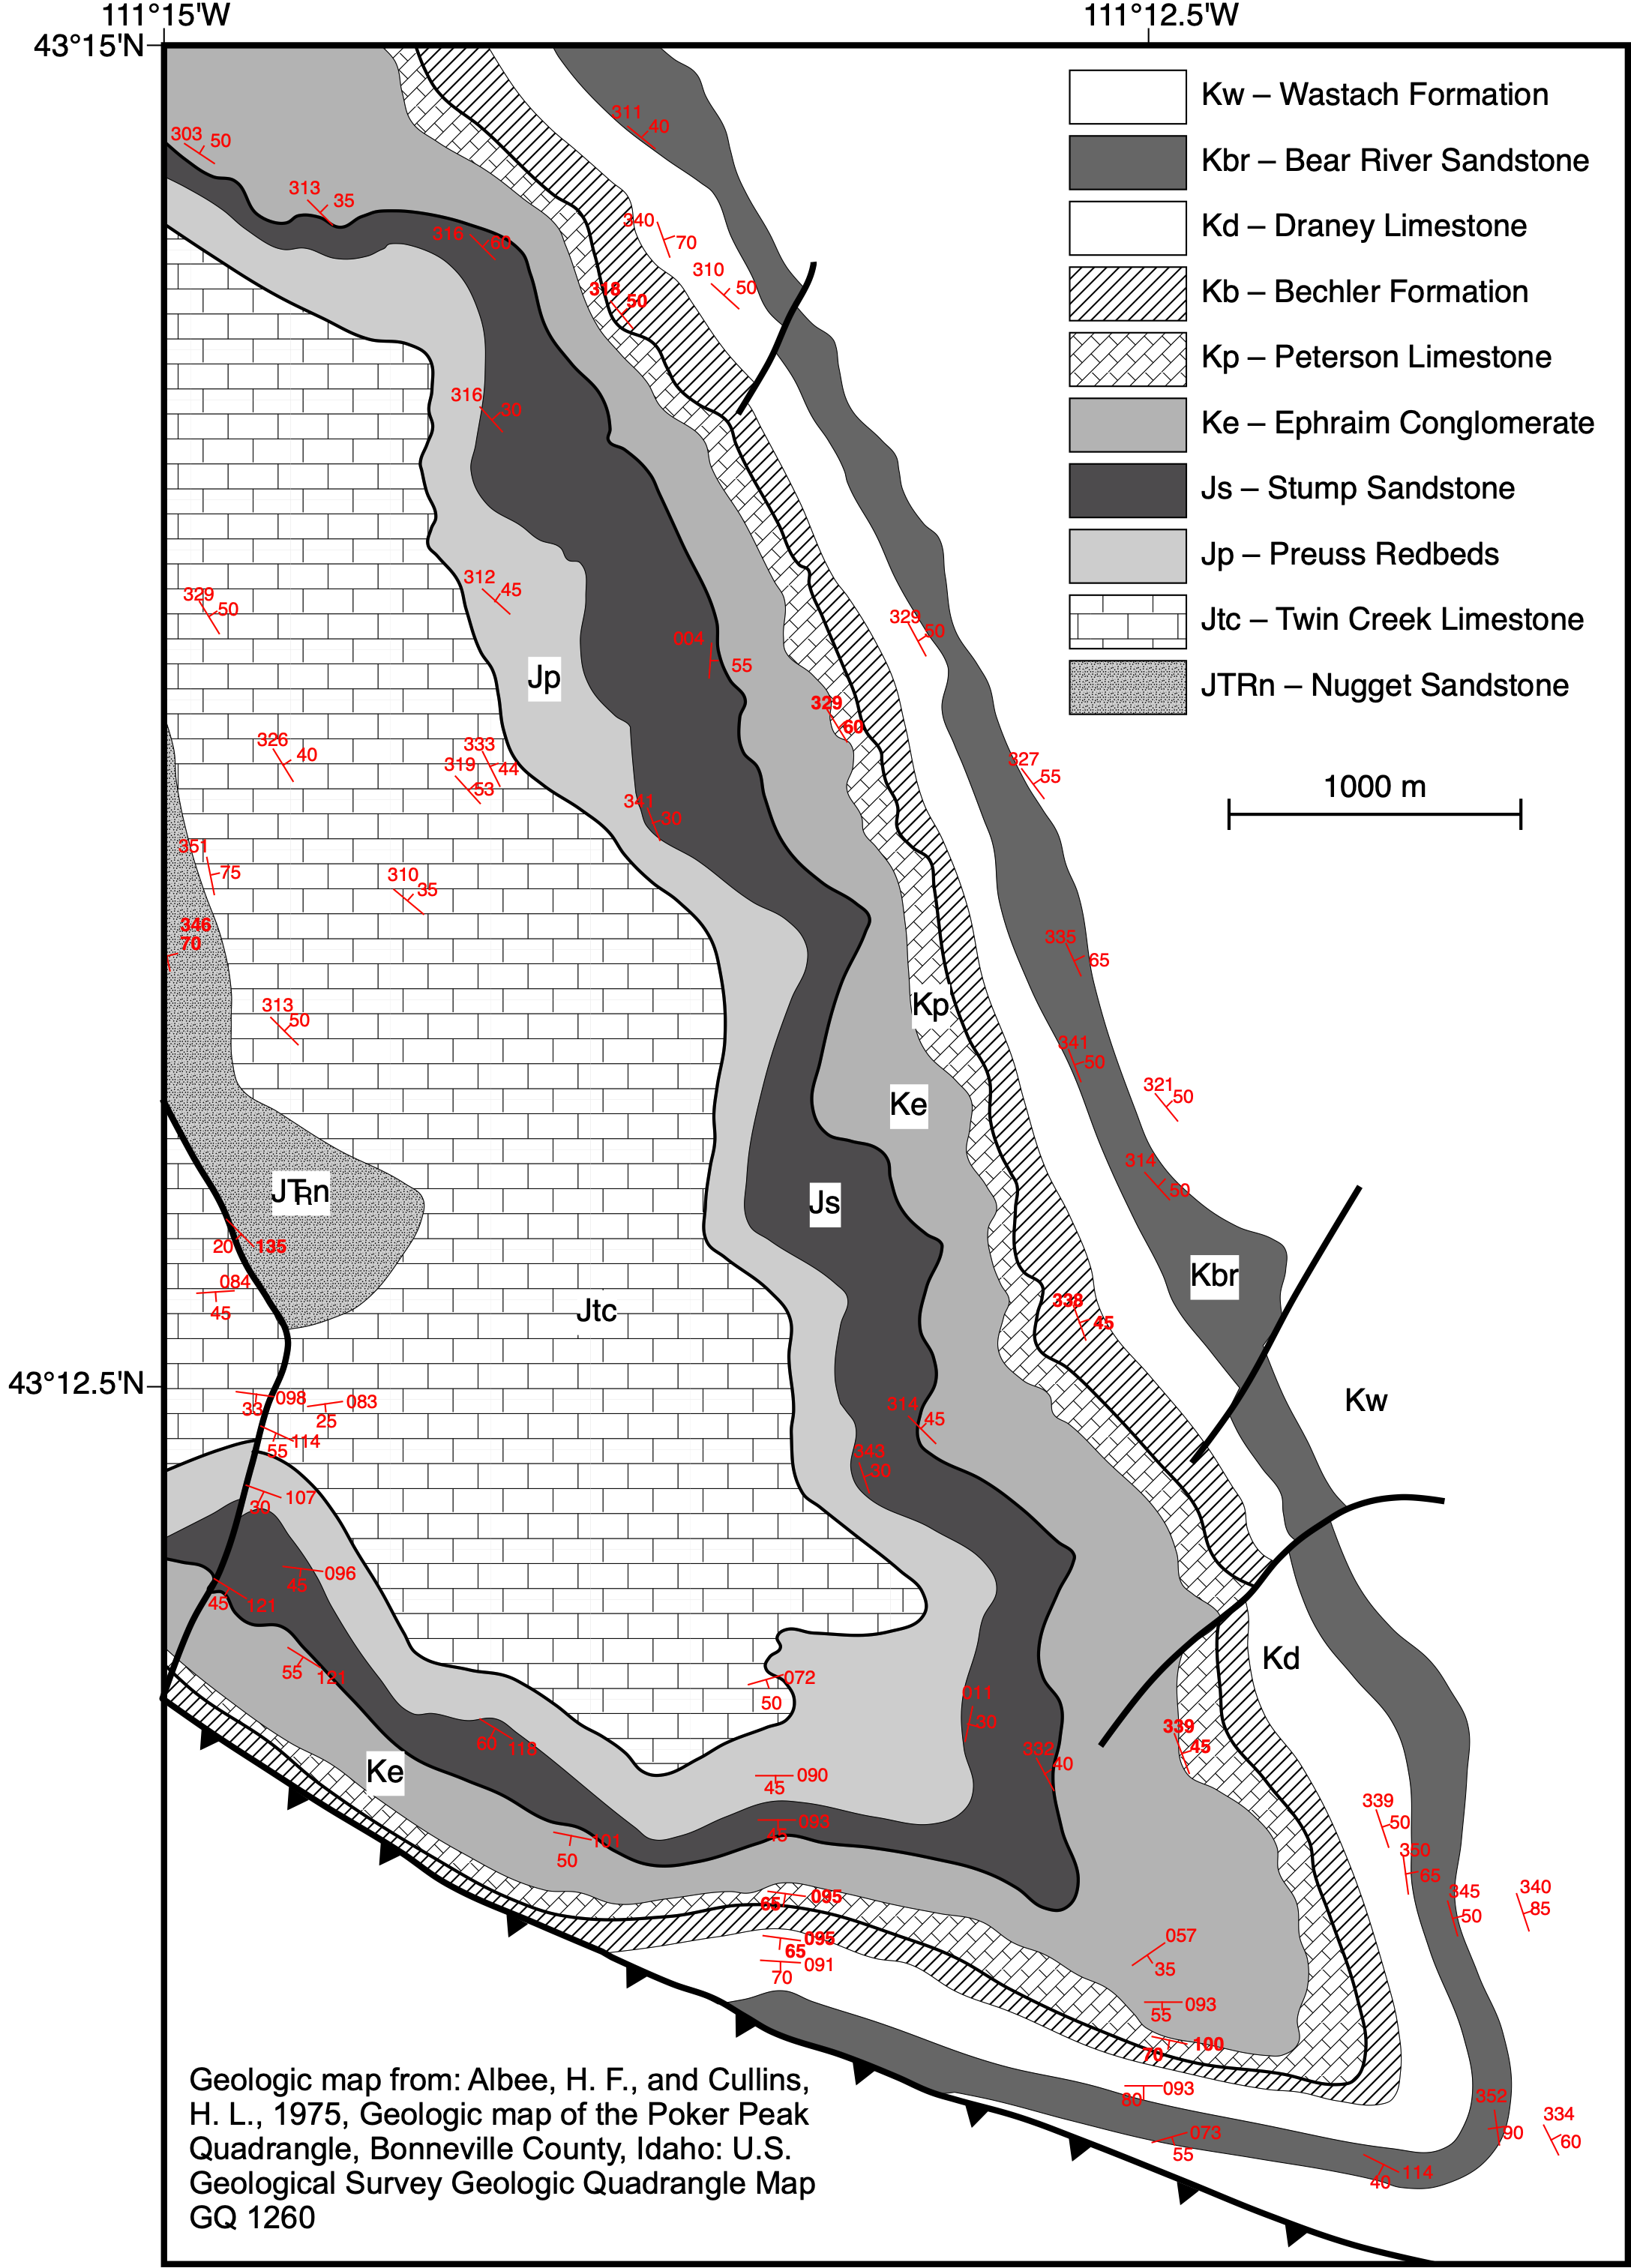
\includegraphics[width=14cm]{Figures/ch5f8.png}
    \caption{Simplified geologic map of the Big Elk anticline in southeastern Idaho. Modified from Allmendinger et al. (2012).}
\end{figure}

\begin{center}
\fbox{
    \parbox{\textwidth - 2 \fboxsep}{
    Output: \\
    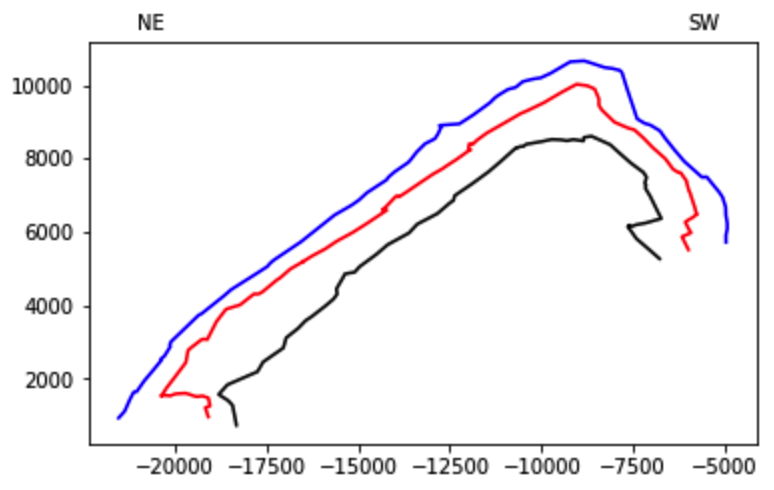
\includegraphics[width=10cm]{Figures/ch5f9.png}
}}
\end{center}

The thrust verges to the NE (the direction of transport is towards the NE), yet the fold verges to the SW in the opposite direction. Unit Jp, between Jtc and Js, contains evaporites (Fig. 5.7). Could this explain the observed fold geometry?

\subsection{Rotations}

Rotations are essential in geology. For example, when we measure the orientation of current lineations on tilted beds, and we want to estimate the orientation of the paleo-current that deposited these beds, we need to rotate or unfold the beds (and the lineations) back to their pre-tilting orientation. The stereonet is a convenient device to rotate data around a horizontal axis or a vertical axis, but it is rather difficult to rotate data around an axis of a different orientation (Marshak and Mitra, 1988). 

A rotation is also a coordinate transformation from an old coordinate system $\mathbf{X_1}\mathbf{X_2}\mathbf{X_3}$ to a new coordinate system $\mathbf{X_1\text{$'$}}\mathbf{X_2\text{$'$}}\mathbf{X_3\text{$'$}}$ (Fig. 5.8). The rotation axis is specified by its trend and plunge, and the magnitude of rotation is given as an angle $\omega$ that is positive if the rotation is clockwise about the given axis and vice versa (Fig. 5.8). The difficult part is that the rotation axis may not coincide with the axes of either the old or the new coordinate system (unlike the Down-Plunge projection).

The components of the transformation matrix \textbf{a} defining the rotation, which are the direction cosines of the new coordinate system $\mathbf{X_1\text{$'$}}\mathbf{X_2\text{$'$}}\mathbf{X_3\text{$'$}}$ with regards to the old coordinate system $\mathbf{X_1}\mathbf{X_2}\mathbf{X_3}$, can be found using spherical trigonometry (Allmendinger et al., 2012) or linear algebra as we did before. Here, we give them without proof. If $\cos\alpha$, $\cos\beta$ and $\cos\gamma$ are the direction cosines of the rotation axis in the \textbf{NED} coordinate system (Table 4.1), and $\omega$ is the amount of rotation, the elements of matrix \textbf{a} are:

\begin{equation}
    \begin{split}
        a_{11}=\cos\omega+\cos^2\alpha(1-\cos\omega) \hspace{30pt} \\
        a_{12}=-\cos\gamma\sin\omega+\cos\alpha\cos\beta(1-\cos\omega) \\
        a_{13}=\cos\beta\sin\omega+\cos\alpha\cos\gamma(1-\cos\omega) \hspace{7pt} \\
        a_{21}=\cos\gamma\sin\omega+\cos\beta\cos\alpha(1-\cos\omega) \hspace{7pt} \\
        a_{22}=\cos\omega+\cos^2\beta(1-\cos\omega) \hspace{30pt} \\
        a_{23}=-\cos\alpha\sin\omega+\cos\beta\cos\gamma(1-\cos\omega) \\
        a_{31}=-\cos\beta\sin\omega+\cos\gamma\cos\alpha(1-\cos\omega) \\
        a_{32}=\cos\alpha\sin\omega+\cos\gamma\cos\beta(1-\cos\omega) \hspace{7pt} \\
        a_{33}=\cos\omega+\cos^2\gamma(1-\cos\omega) \hspace{30pt}
    \end{split}
\end{equation}

The function \href{https://github.com/nfcd/compGeo/blob/master/source/functions/Rotate.py}{\textit{Rotate}} rotates a line (\textit{trd} and \textit{plg}) about a rotation axis (\textit{rtrd} and \textit{rplg}), an amount $\omega$ (\textit{rot}):

\begin{lstlisting}[language=Python, frame=single]
import numpy as np
from SphToCart import SphToCart as SphToCart
from CartToSph import CartToSph as CartToSph

def Rotate(rtrd,rplg,rot,trd,plg,ans0):
    '''
	Rotate rotates a line by performing a coordinate 
	transformation. The algorithm was originally written 
	by Randall A. Marrett

	rtrd = trend of rotation axis
	rplg = plunge of rotation axis
	rot = magnitude of rotation
	trd = trend of the vector to be rotated
	plg = plunge of the vector to be rotated
	ans0 = A character indicating whether the line to be rotated 
	is an axis (ans0 = 'a') or a vector (ans0 = 'v')

	NOTE: All angles are in radians
	
	Rotate uses functions SphToCart and CartToSph
	
	Python function translated from the Matlab function 
	Rotate in Allmendinger et al. (2012)
	'''
    # Allocate some arrays
    a = np.zeros((3,3)) #'Transformation matrix
    pole = np.zeros(3) #'Direction cosines of rotation axis
    plotr = np.zeros(3) #'Direction cosines of rotated vector
    temp = np.zeros(3)  #'Direction cosines of unrotated vector
    
    # Convert rotation axis to direction cosines. Note that the 
    # convention here is X1 = North, X2 = East, X3 = Down
    pole[1] , pole[2], pole[3] = SphToCart(rtrd,rplg,0)
    
    # Calculate the transformation matrix a for the rotation
    # Eq. 5.17
    x = 1.0 - np.cos(rot)
    sinRot = np.sin(rot)
    cosRot = np.cos(rot)
    a[1,1] = cosRot + pole[1]*pole[1]*x
    a[1,2] = -pole[3]*sinRot + pole[1]*pole[2]*x
    a[1,3] = pole[2]*sinRot + pole[1]*pole[3]*x
    a[2,1] = pole[3]*sinRot + pole[2]*pole[1]*x
    a[2,2] = cosRot + pole[2]*pole[2]*x
    a[2,3] = -pole[1]*sinRot + pole[2]*pole[3]*x
    a[3,1] = -pole[2]*sinRot + pole[3]*pole[1]*x
    a[3,2] = pole[1]*sinRot + pole[3]*pole[2]*x
    a[3,3] = cosRot + pole[3]*pole[3]*x
    
    
    # Convert trend and plunge of vector to be rotated into 
    # direction cosines
    temp[1] , temp[2], temp[3] = SphToCart(trd,plg,0)
    
    # Perform the coordinate transformation
    for i in range(0,3,1):
        plotr[i] = 0.0
        for j in range(0,3,1):
            plotr[i] = a[i,j]*temp[j] + plotr[i]
            
    # Convert to lower hemisphere projection if data are
    # axes (ans0 = 'a')
    if plotr[3] < 0.0 and ans0 == 'a' :
        plotr[1] = -plotr[1]
        plotr[2] = -plotr[2]
        plotr[3] = -plotr[3]
        
    # Convert from direction cosines back to trend and plunge
    rtrd , rplg = CartToSph(plotr[1], plotr[2], plotr[3])
    
    return rtrd, rplg
\end{lstlisting}

The  notebook  \href{https://github.com/nfcd/compGeo/blob/master/source/notebooks/ch5-5.ipynb}{ch5-5} illustrates  the  use  of  the  function \textit{Rotate} to solve the following problem from Leyshon  and Lisle  (1996): An overturned bed oriented 305/60 (RHR) has sedimentary lineations which indicate the palaeocurrent direction. These pitch at 60NW, with the current flowing up the plunge. Calculate the original trend of the palaeocurrents. 

Besides rotating the lineations back to their pre-tilted orientation, there is an additional challenge in this problem. We need to figure out the orientation of the lineations from their pitch on the bed. We will do this as well using a rotation.

\begin{center}
\begin{lstlisting}[language=Python, frame=single]
import math
pi = math.pi

import sys
import os
sys.path.append(os.path.abspath('../functions'))
from Pole import Pole as Pole
from Rotate import Rotate as Rotate
from ZeroTwoPi import ZeroTwoPi as ZeroTwoPi

# Strike and dip of bed in radians
strike = 305*pi/180
dip = 60*pi/180

# Pole of bed
rtrd, rplg = Pole(strike, dip, 1)

# To find the orientation of the lineations
# rotate the strike line clockwise about the 
# pole an amount equal to the pitch

# strike line
trd = strike 
plg = 0

# rotation = pitch in radians
rot = 60 * pi/180 

# orientation of lineations
trdr, plgr = Rotate(rtrd,rplg,rot,trd,plg,'a')

# Now we need to rotate the lineations about
# the strike line to their pre-tilted orientation

# The bed is overturned, so it has been rotated 
# pass the vertical. The amount of rotation
# required to restore the bed to its pre-tilted
# orientation is 180- 60 = 120 deg, and it
# should be clockwise
rot = 120 * pi/180 # rotation in radians

# rotate lineations to their pre-tilted orientation
trdl, plgl = Rotate(trd,plg,rot,trdr,plgr,'a')

# The current flows up the plunge, 
# so the trend of the paleocurrents is:
trdl = ZeroTwoPi(trdl + pi)
print('Original trend of the paleocurrents = {:.1f}'.format(trdl*180/pi))
\end{lstlisting}
\fbox{
    \parbox{\textwidth - 2 \fboxsep}{
    Output: \\
    Original trend of the paleocurrents = 65.0
}}
\end{center}

\subsection{Plotting great and small circles using rotations}

The transformation matrix \textbf{a} that describes the rotation (Eq. 5.17), provides a simple and elegant way to draw great and small circles on a stereonet. As you may suspect from the previous notebook, to draw a great circle, we just need to rotate the strike line of the plane in fixed increments (e.g. 1\degree) around the pole to the plane until completing 180\degree. This is the same as drawing lines on the plane of incrementally larger rake from 0 to 180\degree. To draw a small circle, we just need to incrementally rotate (e.g. 1\degree increments) a line around the axis of the conic section until completing 360\degree. Any line making an angle less than 90\degree with the axis of rotation will trace out a cone, which plots on the stereonet as a small circle. The functions \href{https://github.com/nfcd/compGeo/blob/master/source/functions/GreatCircle.py}{\textit{GreatCircle}} and \href{https://github.com/nfcd/compGeo/blob/master/source/functions/SmallCircle.py}{\textit{SmallCircle}} return the path of great and small circles on an equal angle or equal area stereonet:

\begin{lstlisting}[language=Python, frame=single]
import numpy as np
from Pole import Pole as Pole
from Rotate import Rotate as Rotate
from StCoordLine import StCoordLine as StCoordLine

def GreatCircle(strike,dip,sttype):
    '''
	GreatCircle computes the great circle path of a plane 
	in an equal angle or equal area stereonet of unit radius
	
	strike = strike of plane
	dip = dip of plane
	sttype = type of stereonet: 0 = equal angle, 1 = equal area
	path = x and y coordinates of points in great circle path
	
	NOTE: strike and dip should be entered in radians. 
	
	GreatCircle uses functions StCoordLine, Pole and Rotate
	
	Python function translated from the Matlab function
	GreatCircle in Allmendinger et al. (2012)
	'''
    pi = np.pi
	# Compute the pole to the plane. This will be the axis of 
	# rotation to make the great circle
    trda, plga = Pole(strike,dip,1)
    
	# Now pick the strike line at the intersection of the 
    # great circle with the primitive of the stereonet
    trd = strike
    plg = 0.0
    
	# To make the great circle, rotate the line 180 degrees 
	# in increments of 1 degree
    rot = np.arange(0,181,1)*pi/180
    path = np.zeros((rot.shape[0],2))
    
    for i in range(rot.shape[0]):
	# Avoid joining ends of path
        if rot[i] == pi:
            rot[i] = rot[i]*0.9999
		# Rotate line
        rtrd, rplg = Rotate(trda,plga,rot[i],trd,plg,'a')
		# Calculate stereonet coordinates of rotated line 
		# and add to great circle path
        path[i,0], path[i,1] = StCoordLine(rtrd,rplg,sttype)
    
    return path
\end{lstlisting}

\begin{lstlisting}[language=Python, frame=single]
import numpy as np
from Rotate import Rotate as Rotate
from StCoordLine import StCoordLine as StCoordLine
from ZeroTwoPi import ZeroTwoPi as ZeroTwoPi

def SmallCircle(trda,plga,coneAngle,sttype):
    '''
	SmallCircle computes the paths of a small circle defined 
	by its axis and cone angle, for an equal angle or equal 
	area stereonet of unit radius
	
	trda = trend of axis
	plga = plunge of axis
	coneAngle = cone angle
	sttype = type of stereonet. 0 = equal angle, 1 = equal area
	path1 and path2 are vectors with the x and y coordinates of 
       the points in the small circle paths
       np1 and np2 = Number of points in path1 and path2
       
    NOTE: All angles should be in radians

	SmallCircle uses functions ZeroTwoPi, StCoordLine and Rotate

	Python function translated from the Matlab function 	
	SmallCircle in Allmendinger et al. (2012)
	'''
    pi = np.pi
	# Find where to start the small circle
    if (plga - coneAngle) >= 0.0:
        trd = trda
        plg = plga - coneAngle
    else:
        if plga == pi/2.0:
            plga = plga*0.9999
        angle = np.arccos(np.cos(coneAngle)/np.cos(plga))
        trd = ZeroTwoPi(trda+angle)
        plg = 0.0
    
    
	# To make the small circle, rotate the starting line 
	# 360 degrees in increments of 1 degree
    rot = np.arange(0,361,1)*pi/180
    path1 = np.zeros((rot.shape[0],2))
    path2 = np.zeros((rot.shape[0],2))
    np1 = 0
    np2 = 0
    for i in range(rot.shape[0]):
        # Rotate line: Notice that the line is considered as a vector
        rtrd , rplg = Rotate(trda,plga,rot[i],trd,plg,'v')
        # Add to the right path
        # If plunge of rotated line is positive add to first path
        if rplg >= 0.0:
            # Calculate stereonet coordinates and add to path
            path1[np1,0] , path1[np1,1] = StCoordLine(rtrd,rplg,sttype)
            np1 = np1 +1
        else:
            path2[np2,0] , path2[np2,1] = StCoordLine(rtrd,rplg,sttype)
            np2 = np2 +1
    
    return path1, path2, np1, np2
\end{lstlisting}

Normally, stereonets are displayed with the primitive equal to the horizontal (i.e. looking straight down). However, sometimes is convenient to look at the stereonet in another orientation. For example, one may want to plot data in the plane of a cross section (the view direction is perpendicular to the cross section), or in a down-plunge projection of a fold (the view direction is parallel to the fold axis). The function \href{https://github.com/nfcd/compGeo/blob/master/source/functions/GeogrToView.py}{\textit{GeogrToView}} enables to plot great and small circles on a stereonet of any view direction, by transforming the poles of rotation from \textbf{NED} coordinates to the view direction coordinates:

\begin{lstlisting}[language=Python, frame=single]
import numpy as np
from SphToCart import SphToCart as SphToCart
from CartToSph import CartToSph as CartToSph
from ZeroTwoPi import ZeroTwoPi as ZeroTwoPi

def GeogrToView(trd,plg,trdv,plgv):
    '''
	GeogrToView transforms a line from NED to View Direction
	coordinates
	trd = trend of line
   	plg = plunge of line 
   	trdv = trend of view direction 
   	plgv = plunge of view direction 
   	rtrd and rplg are the new trend and plunge of the line 
   	in the view direction.

   	NOTE: Input/Output angles are in radians

   	GeogrToView uses functions ZeroTwoPi, SphToCart and CartToSph

   	Python function translated from the Matlab function 
   	GeogrToView in Allmendinger et al. (2012)
	'''
    #some constants 
    east = np.pi/2.0
    
    #Make transformation matrix between NED and View Direction
    a = np.zeros((3,3))
    a[2,0], a[2,1], a[2,2] = SphToCart(trdv,plgv,0)
    temp1 = trdv + east
    temp2 = 0.0
    a[1,0], a[1,1], a[1,2] = SphToCart(temp1,temp2,0)
    temp1 = trdv
    temp2 = plgv - east
    a[0,0], a[0,1], a[0,2] = SphToCart(temp1,temp2,0)
     
    #Direction cosines of line
    dirCos = np.zeros(3)
    dirCos[0], dirCos[1], dirCos[2] = SphToCart(trd,plg,0)
      
    # Transform line
    nDirCos = np.zeros(3)
    for i in range(0,3,1):
        nDirCos[i] = a[i,0]*dirCos[0] + a[i,1]*dirCos[1]+ a[i,2]*dirCos[2]
    
    # Compute line from new direction cosines
    rtrd, rplg = CartToSph(nDirCos[0],nDirCos[1],nDirCos[2])
    
    # Take care of negative plunges
    if rplg < 0.0 :
        rtrd = ZeroTwoPi(rtrd+np.pi)
        rplg = -rplg
    
    return rtrd, rplg
\end{lstlisting}

We put these three functions together in a function called \href{https://github.com/nfcd/compGeo/blob/master/source/functions/Stereonet.py}{\textit{Stereonet}}, that plots an equal angle or equal area stereonet in any view direction:

\begin{lstlisting}[language=Python, frame=single]
import numpy as np
import matplotlib.pyplot as plt
from Pole import Pole as Pole
from GeogrToView import GeogrToView as GeogrToView
from SmallCircle import SmallCircle as SmallCircle
from GreatCircle import GreatCircle as GreatCircle

def Stereonet(trdv,plgv,intrad,sttype):
    '''
	Stereonet plots an equal angle or equal area stereonet 
	of unit radius in any view direction
	
	trdv = trend of view direction
	plgv = plunge of view direction
	intrad = interval in radians between great or small circles 
	sttype = type of stereonet. 0 = equal angle, 1 = equal area
	
	NOTE: All angles should be entered in radians
	
	Stereonet uses functions Pole, GeogrToView, 
	SmallCircle and GreatCircle
	
	Python function translated from the Matlab function
	Stereonet in Allmendinger et al. (2012)
	'''
    pi = np.pi
    # some constants
    east = pi/2.0
    west = 3.0*east
    
    # Plot stereonet reference circle
    r = 1.0 # radius pf stereonet
    TH = np.arange(0,360,1)*pi/180
    X = r * np.cos(TH)
    Y = r * np.sin(TH)
    
    # Make a larger figure
    plt.rcParams['figure.figsize'] = [15, 7.5]
    plt.plot(X,Y, 'k')
    plt.axis ([-1, 1, -1, 1])
    plt.axis ('equal')
    plt.axis('off')
    
    # Number of small circles
    nCircles = int(pi/(intrad*2.0))
    
    # small circles
    # start at the North
    trd = 0.0
    plg = 0.0
    
    # If view direction is not the default (trdv=0,plgv=90)
    # transform line to view direction
    if trdv != 0.0 and plgv != east:
        trd, plg = GeogrToView(trd,plg,trdv,plgv)
    
    # Plot small circles
    for i in range(1,nCircles+1):
        coneAngle = i*intrad
        path1, path2, np1, np2 = SmallCircle(trd,plg,coneAngle,sttype)
        plt.plot(path1[np.arange(0,np1),0], path1[np.arange(0,np1),1], color='gray',linewidth=0.5)
        if np2 > 0:
            plt.plot(path2[np.arange(0,np2),0], path2[np.arange(0,np2),1], color='gray', linewidth=0.5)
    
    # Great circles
    for i in range(0,nCircles*2+1):
        # Western half
        if i <= nCircles:
            # Pole of great circle
            trd = west
            plg = i*intrad
            # Eastern half
        else:
            # Pole of great circle
            trd = east
            plg = (i-nCircles)*intrad
        # If pole is vertical, shift it a little bit
        if plg == east:
            plg = plg * 0.9999
        # If view direction is not the default (trdv=0,plgv=90)
        # transform line to view direction
        if trdv != 0.0 and plgv != east:
            trd, plg = GeogrToView(trd,plg,trdv,plgv)
        # Compute plane from pole
        strike, dip = Pole(trd,plg,0)
        # Plot great circle
        path = GreatCircle(strike,dip,sttype)
        plt.plot(path[:,0], path[:,1], color='gray', linewidth=0.5)
\end{lstlisting}

Now, let's use all these functions to plot the bedding data of the Big Elk anticline (Fig. 5.7) in an equal angle stereonet, looking down and also along the fold axis. The notebook \href{https://github.com/nfcd/compGeo/blob/master/source/notebooks/ch5-6.ipynb}{ch5-6} illustrates this. Notice that we read the strike and dips from the file \href{https://github.com/nfcd/compGeo/blob/master/source/data/ch5-6/beasd.txt}{\textit{beasd.txt}}:

\begin{center}
\begin{lstlisting}[language=Python, frame=single]
import numpy as np
import matplotlib.pyplot as plt
%matplotlib  inline
pi = np.pi

import sys
import os
sys.path.append(os.path.abspath('../functions'))
from Pole import Pole as Pole
from GreatCircle import GreatCircle as GreatCircle
from GeogrToView import GeogrToView as GeogrToView
from Stereonet import Stereonet as Stereonet

# Draw a lower hemisphere equal angle stereonet
trdv = 0
plgv = 90 * pi/180
intrad = 10 * pi/180
Stereonet(trdv,plgv,intrad,0)

# Read the strike-dip data from the Big Elk anticline
beasd = np.loadtxt('beasd.txt')

# Plot the great circles
for i in range(beasd.shape[0]):
    path = GreatCircle(beasd[i,0]*pi/180,beasd[i,1]*pi/180,0)
    plt.plot(path[:,0], path[:,1], 'b', linewidth=0.5) 
\end{lstlisting}
\fbox{
    \parbox{\textwidth - 2 \fboxsep}{
    Output: \\
    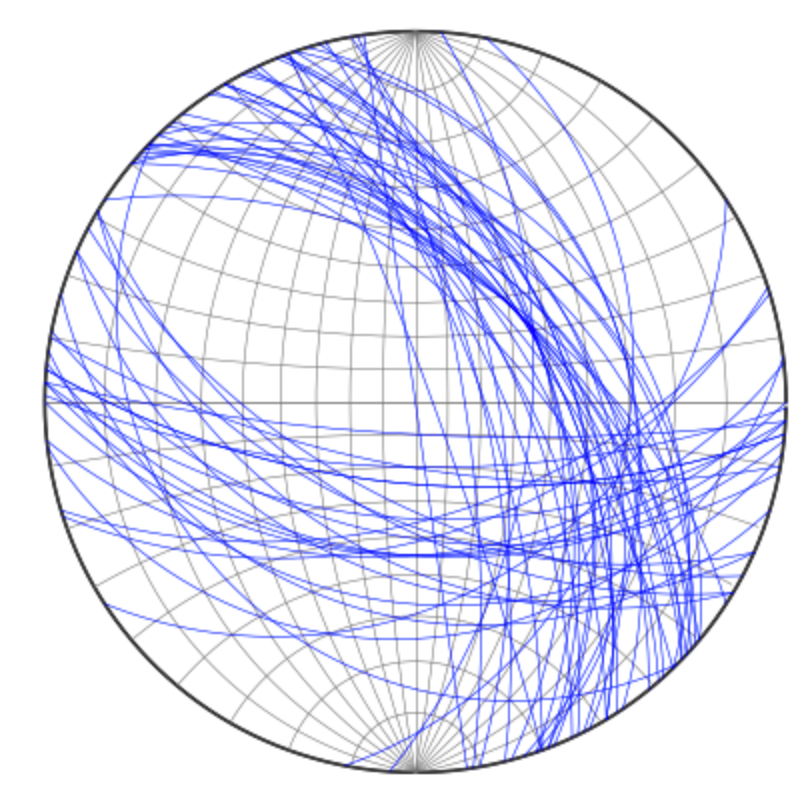
\includegraphics[width=5cm]{Figures/ch5f11.png}
}}
\end{center}

\begin{center}
\begin{lstlisting}[language=Python, frame=single]
# Draw the same data in an equal angle stereonet,
# but make the view direction = fold axis
trdv = 125*pi/180
plgv = 26*pi/180
Stereonet(trdv,plgv,intrad,0)

# Plot the great circles
for i in range(beasd.shape[0]):
    # pole to bed
    trdp, plgp =  Pole(beasd[i,0]*pi/180,beasd[i,1]*pi/180,1)
    # transform pole
    trdpt, plgpt = GeogrToView(trdp,plgp,trdv,plgv)
    # bed from transformed pole
    striket, dipt = Pole(trdpt,plgpt,0)
    # plot great circle
    path = GreatCircle(striket,dipt,0)
    plt.plot(path[:,0], path[:,1], 'b', linewidth=0.5)  
\end{lstlisting}
\fbox{
    \parbox{\textwidth - 2 \fboxsep}{
    Output: \\
    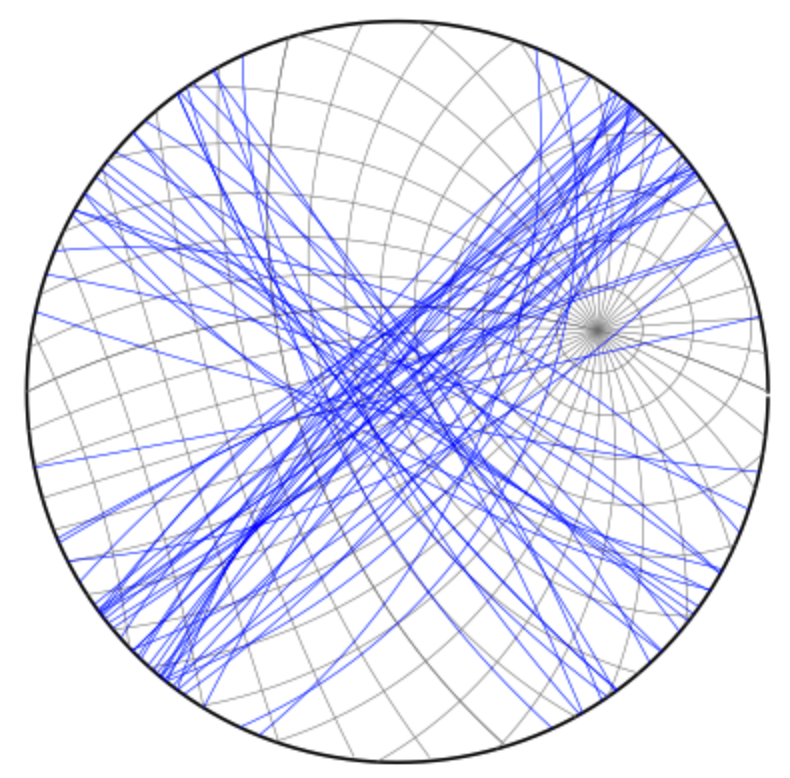
\includegraphics[width=5cm]{Figures/ch5f12.png}
}}
\end{center}

What do these plots tell you about the geometry of the fold?

\section{Exercises}

\begin{enumerate}

    \item Figure 5.8 is a satellite image of the Sheep Mountain anticline, Wyoming, USA (Rioux, 1994). At 75 localities along the anticline in the Jurassic Sundance Formation (gray-green sandstone, siltstone and shale; Rioux, 1994), the \textbf{ENU} coordinates of points on the base and top of the unit (Fig. 5.8a, green and red points), and three points on a bed inside the unit (Fig. 5.8b, blue points), were recorded in Google Earth. You can see these points in Google Earth using the file \href{https://github.com/nfcd/compGeo/blob/master/source/data/ch5-exercise1/sdtp.kml}{\textit{sdtp.kml}}. 
    
    \begin{figure}[ht]
    \centering
    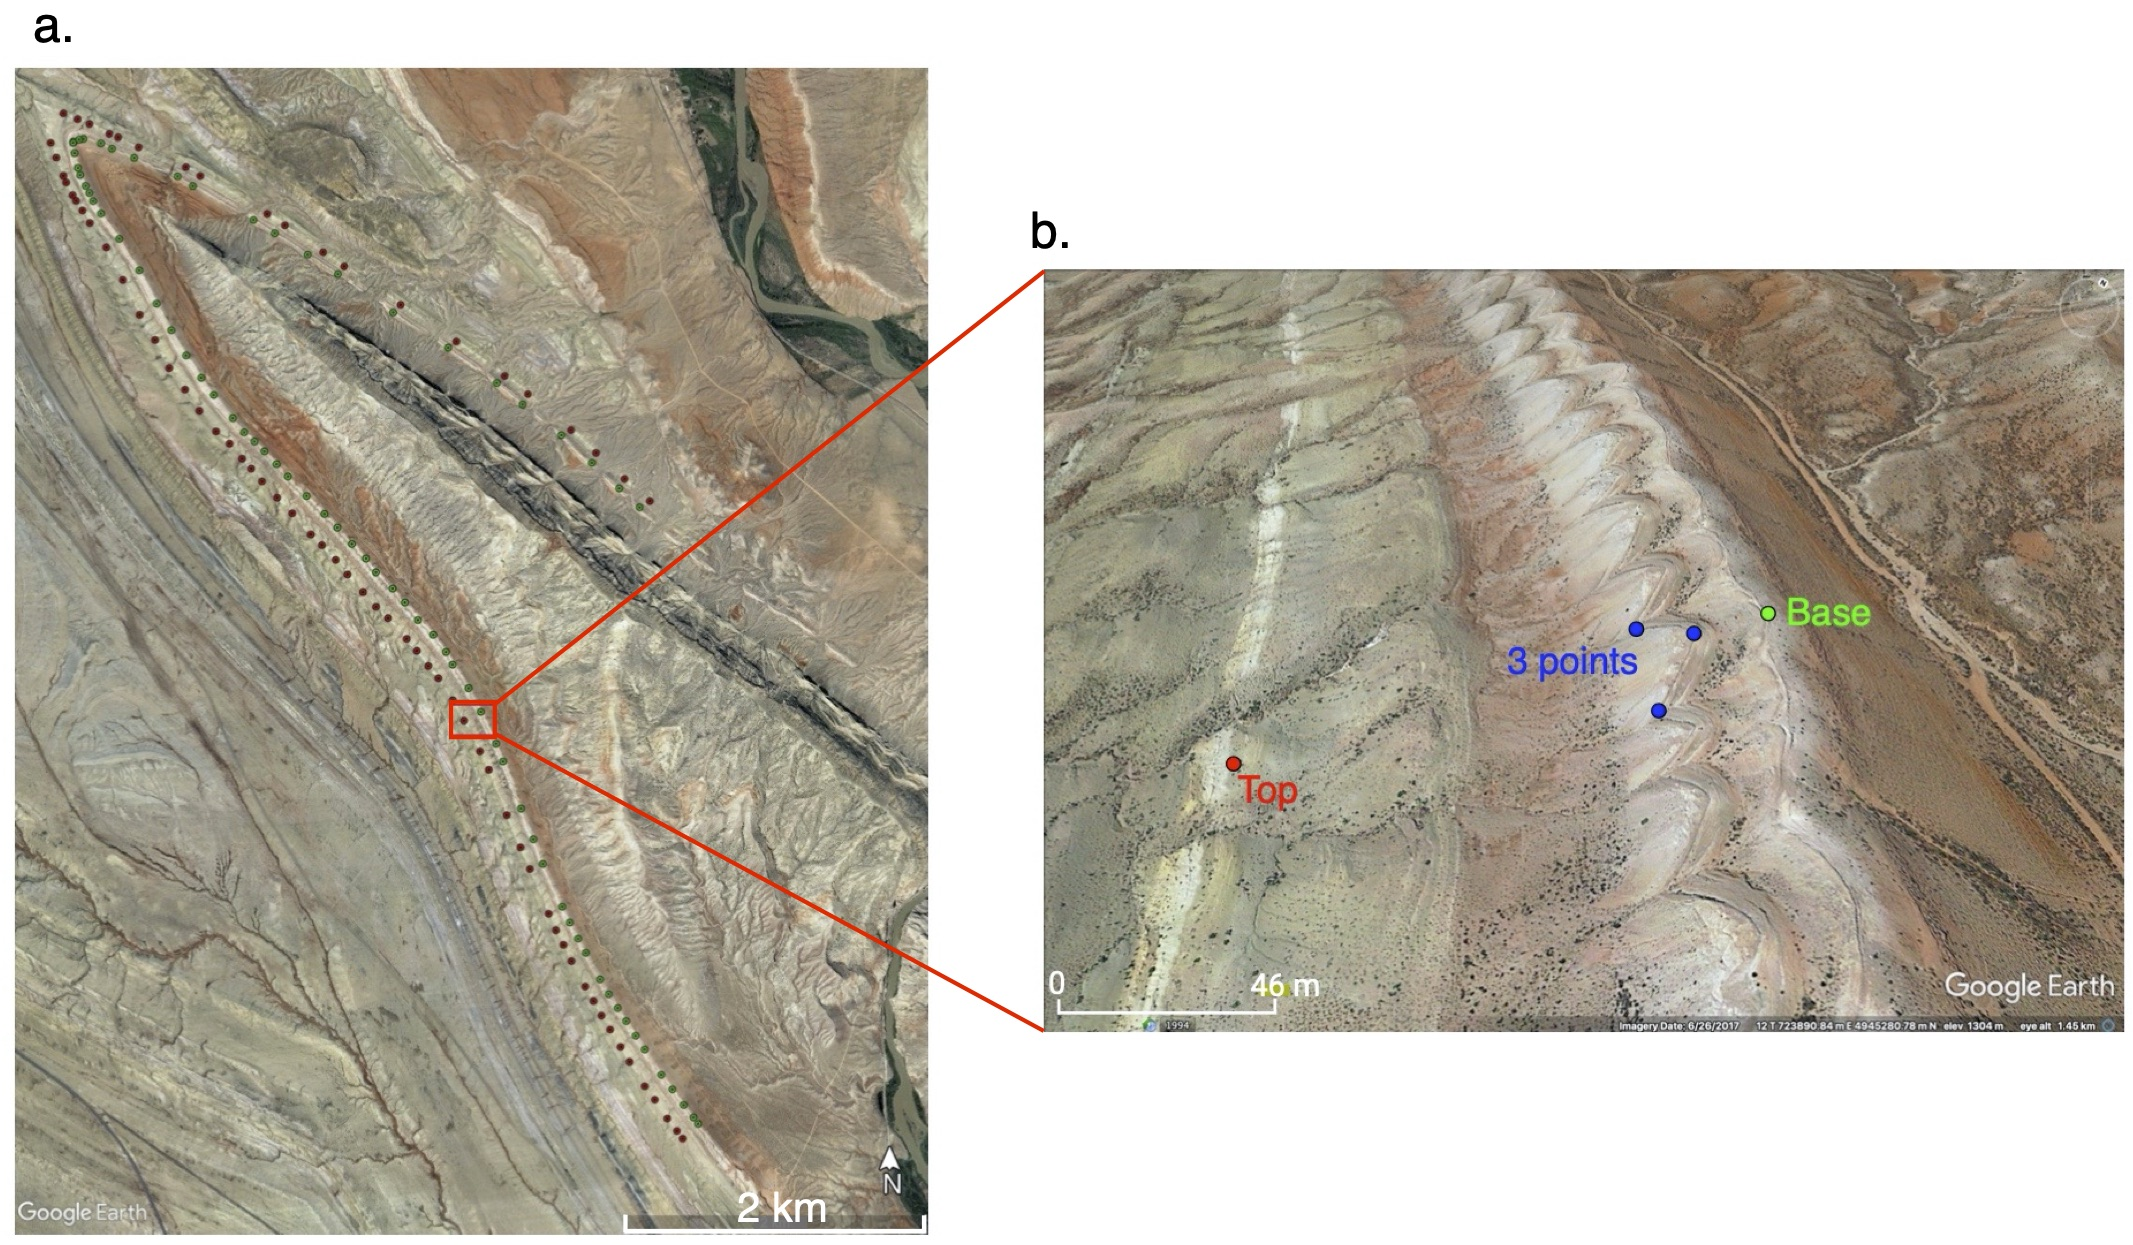
\includegraphics[width=14cm]{Figures/ch5f13.jpg}
    \caption{\textbf{a.} Base (green) and top (red) locations of the Jurassic Sundance Formation along the Sheep Mountain anticline, Wyoming, for exercise 1. \textbf{b.} Closeup of one of the localities (red rectangle in a) showing as well the three points (blue) used to determine strike and dip.}
    \end{figure}
    
    The file \href{https://github.com/nfcd/compGeo/blob/master/source/data/ch5-exercise1/sdtp.txt}{\textit{sdtp.txt}} contains the \textbf{ENU} coordinates (UTM in meters) of the points. Each row is one locality, and it contains 15 columns corresponding to the \textbf{ENU} coordinates of points 1 to 5. Points 1 to 3 are on a bed inside the unit, and points 4 and 5 are on the base and top of the unit, respectively. Columns 1 to 3 are the \textbf{ENU} coordinates of point 1, columns 4 to 6 those of point 2, and so on. 
    
    \begin{enumerate}
        \item Compute the thickness of the Sundance Formation at the 75 localities. Notice that at each locality you will need to compute the strike and dip using points 1-3 and the \textit{ThreePoint} function, and the thickness of the unit using points 4 and 5 and the \textit{TrueThickness} function.
        \item Plot the bedding data along the anticline in and equal area, lower hemisphere stereonet. Plot these data as great circles.
        \item Suppose that the error in horizontal (\textbf{EN}) coordinates is $\pm$ 3 m and in the vertical is $\pm$ 1.5 m. These are conservative error estimates for Google Earth. What are the errors in strike and dip and thickness in the 75 localities? \textit{Hint}: Use functions \textit{ThreePointU} and \textit{TrueThicknessU}.
        \item Make a plot of computed thickness versus computed dip, and another plot of computed thickness versus north (\textbf{N}) for the 75 localities. Include the thickness and dip error bars. Do you see any correlation between thickness and bedding dip? Can you identify any systematic variation of thickness along the anticline? Please consider the errors (uncertainties) when answering these questions. 
        \item The axis of the anticline is oriented 306/11. This is approximately the location where the bedding planes on the stereonet intersect (why?). In the next chapter we will see how to compute this. Make a Down-Plunge projection of the base and top of the Jurassic Sundance Formation. \textit{Hint}: Project the 75 base and top locations using the function \textit{DownPlunge}.
    \end{enumerate}
    
    \item Allmendinger and Judge (2013) wrote an interesting article about the uncertainty in thickness measurements and its implication for estimating the shortening in fold and thrust belts. Figure 5.9 is a geologic map of the Canmore east half area in Alberta, Canada (Price, 1970). The yellow dots in the map are the points used by them to estimate the thickness of the Devonian Palliser (Dpa) and Mississippian Livingstone (Mlv) formations. These are in a homoclinal dip package in a thrust sheet. 
    
     \begin{SCfigure}
        \caption{Geologic map of the Canmore east half area, Alberta, Canada (Price, 1970) for exercise 2. The yellow dots are points used to determine the thickness of the Devonian Palliser (Dpa) and Mississippian Livingstone (Mlv) formations.}
        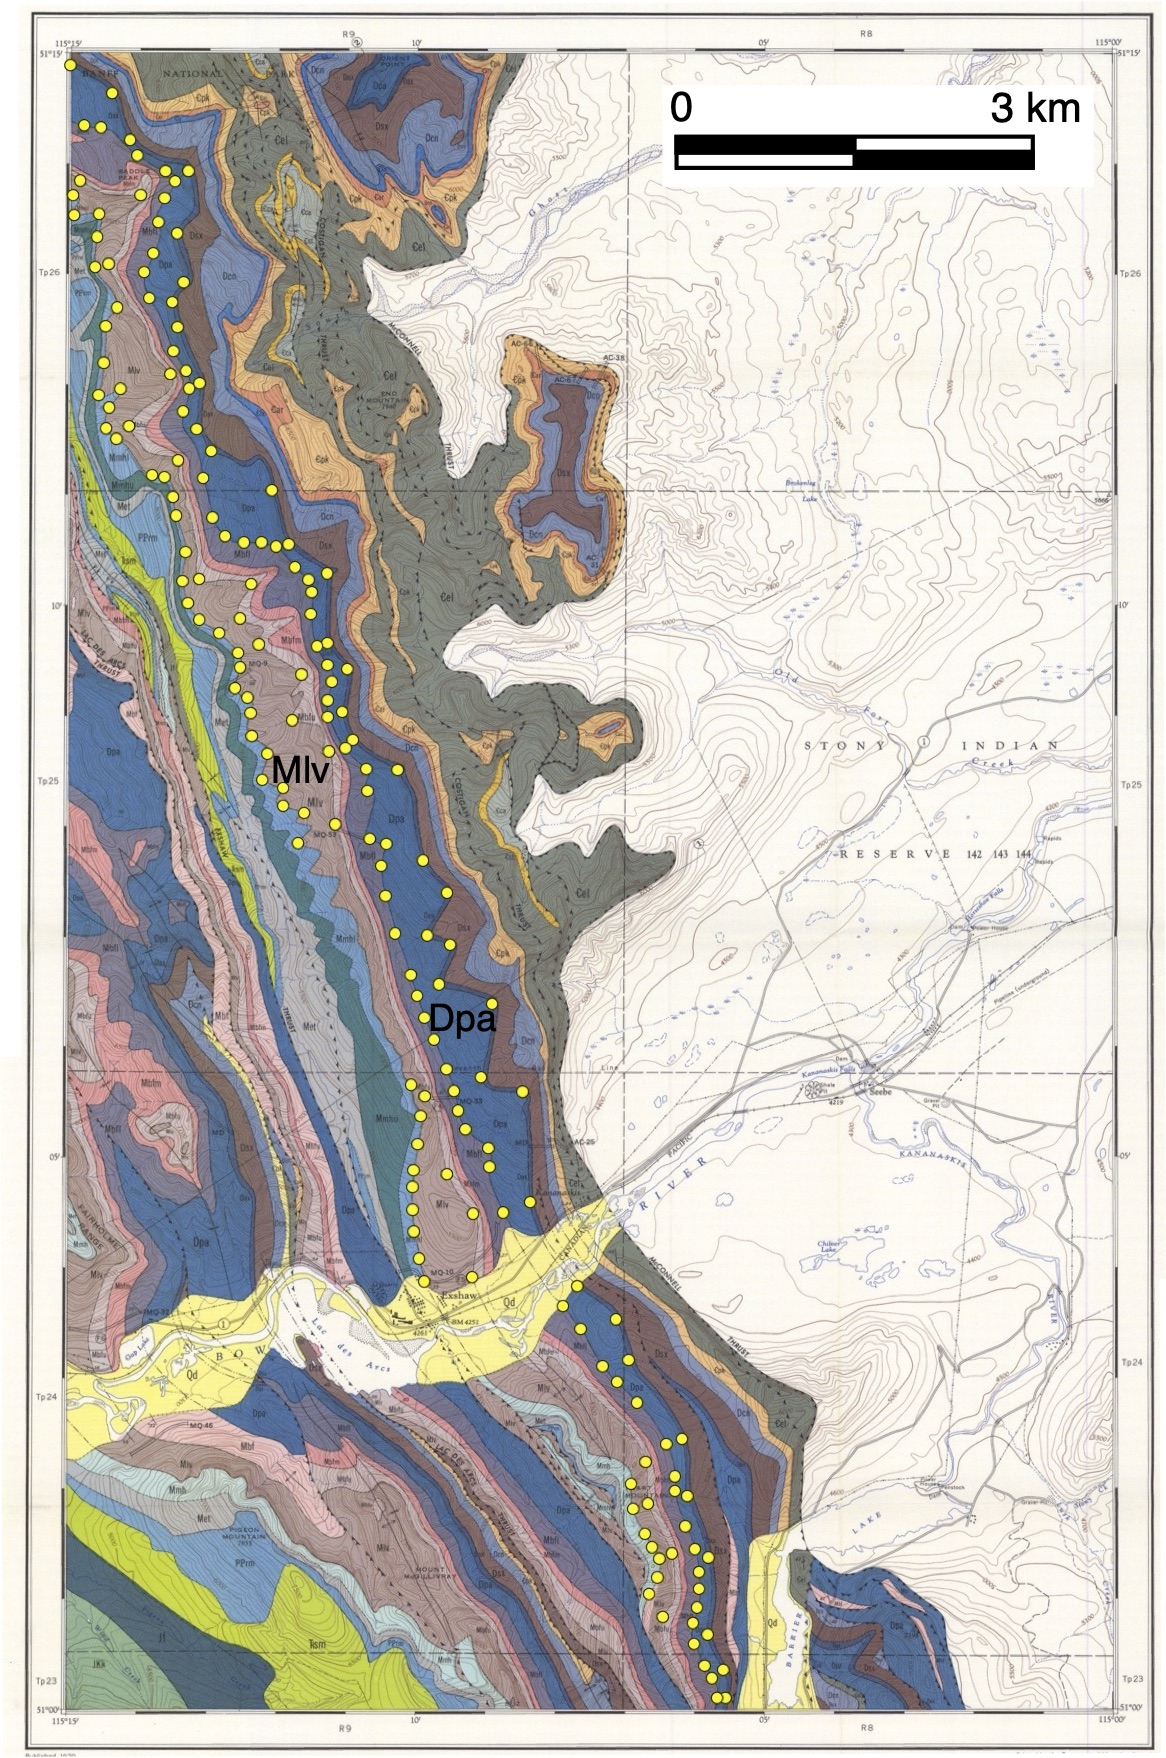
\includegraphics[width=0.5\textwidth]{Figures/ch5f14.jpg}
    \end{SCfigure}
    
    The files \href{https://github.com/nfcd/compGeo/blob/master/source/data/ch5-exercise2/dpa.txt}{\textit{dpa.txt}} and \href{https://github.com/nfcd/compGeo/blob/master/source/data/ch5-exercise2/mlv.txt}{\textit{mlv.txt}} contain the \textbf{ENU} coordinates (UTM in meters) of the points in the Palliser (Dpa) and Livingstone (Mlv) formations, respectively. Each row in the files is one locality, and it contains 12 columns corresponding to the \textbf{ENU} coordinates of points 1 to 4. Points 1-3 are either on the top or the base of the unit, and point 4 is on the other contact. Columns 1 to 3 are the \textbf{ENU} coordinates of point 1, columns 4 to 6 those of point 2, and so on.
    
    \begin{enumerate}
        \item Compute the thickness of the Palliser and Livingstone formations at the localities shown in Figure 5.9. What is the mean value of thickness of these two units? What is the standard deviation (this is also called the 1-sigma error)? \textit{Hint}: Use the functions \textit{ThreePoint} and \textit{TrueThickness}. The NumPy functions \textit{mean} and \textit{std} compute the mean and standard deviation of an array.
        \item Consider that the uncertainty in horizontal and vertical coordinates is $\pm$15.24 m. Compute again the mean value and standard deviation of the thickness of the units. This time these values will have uncertainties. \textit{Hint}: Use the functions \textit{ThreePointU} and \textit{TrueThicknessU}. Notice that you can use the NumPy functions \textit{mean} and \textit{std} on arrays made of numbers with uncertainties (\textit{uFloat}).
        \item How do your results compare to those of Allmendinger and Judge (2013, their Table 1)?
    \end{enumerate}{}
    
    \item The following exercise is from Ragan (2009): With the following information and the topographic map of Fig. 5.10, construct a geological map. The base of a 100 m thick sandstone unit of lower Triassic age is exposed at point A; its attitude is 110/25 (RHR). Point B is on the east boundary of a 50 m thick, vertical diabase dike of Jurassic age; its trend is 020. At point C, the base of a horizontal Cretaceous sequence is exposed and at point D the base of a conformable sequence of Tertiary rocks is present.
    
    \begin{figure}[ht]
    \centering
    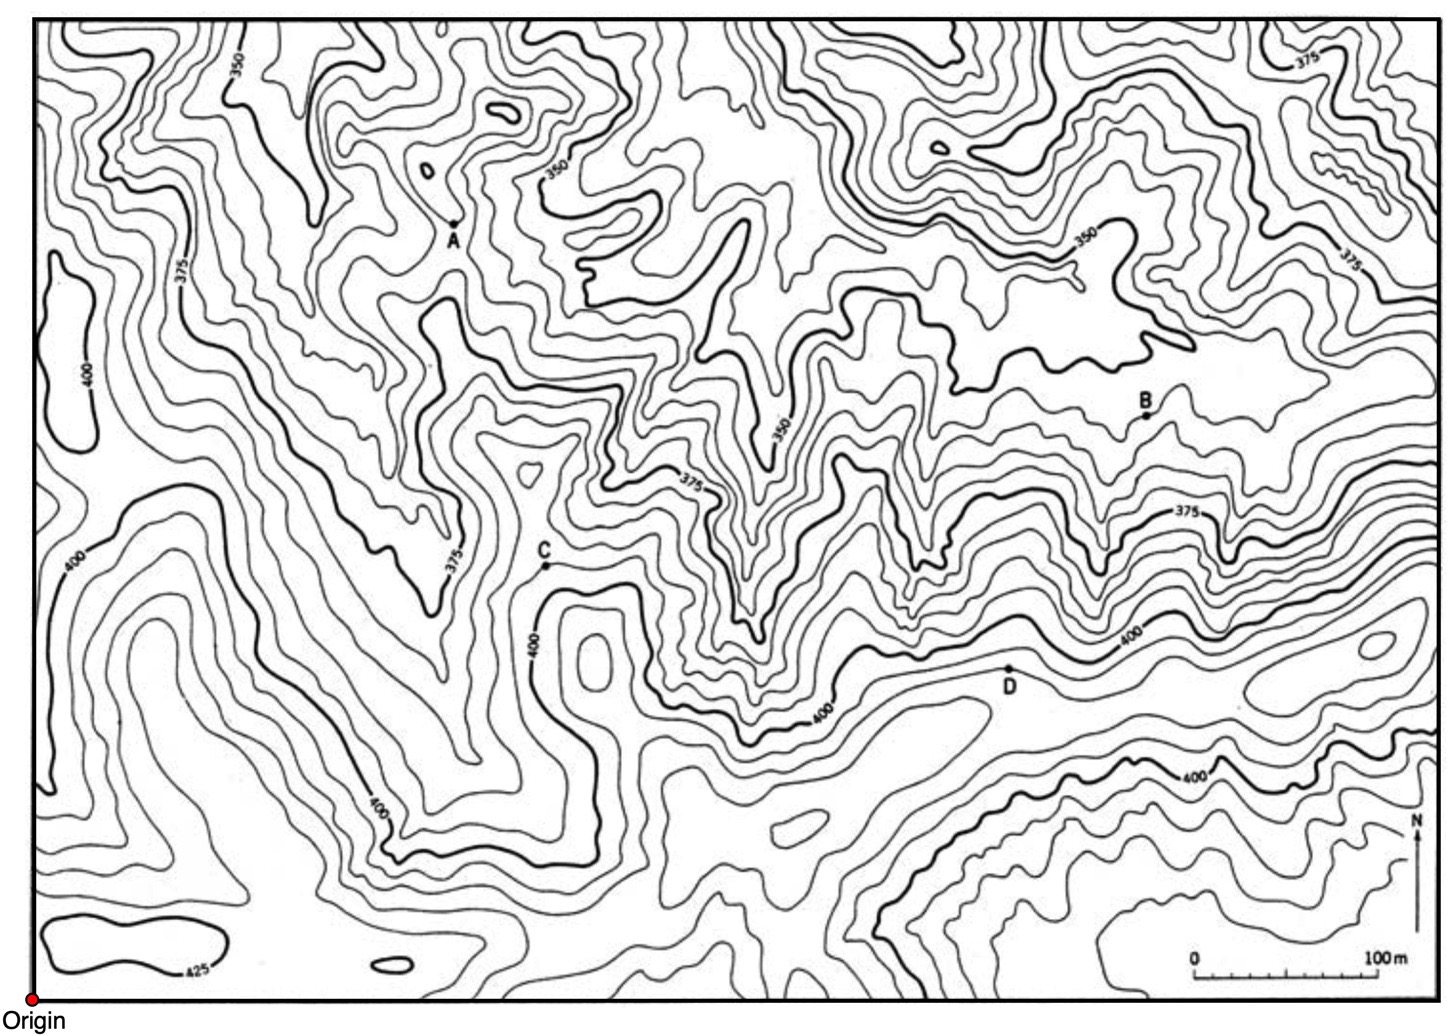
\includegraphics[width=13cm]{Figures/ch5f15.jpg}
    \caption{Topographic map for exercise 3. Notice that the origin is at the lower left corner of the map. This is exercise 2 in chapter 4 of Ragan (2009).}
    \end{figure}
    
    In introductory mapping courses, this exercise is solved graphically (Fig. 3.9). This time, you are going to use computation. The files \href{https://github.com/nfcd/compGeo/blob/master/source/data/ch5-exercise3/XGE.txt}{\textit{XGE.txt}}, \href{https://github.com/nfcd/compGeo/blob/master/source/data/ch5-exercise3/YGE.txt}{\textit{YGE.txt}}, and \href{https://github.com/nfcd/compGeo/blob/master/source/data/ch5-exercise3/ZGE.txt}{\textit{ZGE.txt}} are the \textbf{ENU} coordinates of the points of the DEM grid (these arrays follow the format of the NumPy \textit{meshgrid} function). Points A, B, C and D have the following coordinates \textbf{ENU} coordinates:
    
    A = [232, 428, 370]
    
    B = [612, 322, 355]
    
    C = [281.5, 239, 395]
    
    D = [537, 183, 410]
    
    \textit{Hint}: Use the function \textit{OutcropTrace} to compute the contacts. Follow a procedure similar to notebook \href{https://github.com/nfcd/compGeo/blob/master/source/notebooks/ch5-3.ipynb}{ch5-3} to draw the topographic contours and the contacts. In this case though, some contacts will intersect. At contacts intersections, you will need to use the principle of superposition to determine which contact cuts the other one: e.g. the Jurassic dyke will cut the Triassic sequence, but it will be covered by the Cretaceous and Tertiary sequences.
    
    \item This exercise is from Marshak and Mitra (1988). It's probably one of the hardest exercises to solve using rotations on a stereonet. Here, you will use the function \textit{Rotate} to solve this problem:
    
    In eastern New York, there is an important unconformity called the Taconic unconformity. It separates Mid-Ordovician flysch from Devonian limestone. At a locality near the town of Catskill, the limestone (and the unconformity) is oriented 195/44 (RHR). An anticline occurs in the underlying flysch. One limb is presently oriented 240/73 (limb 1), and the other limb is presently oriented 020/41 (limb 2) (RHR). Flute casts occur in the Ordovician strata on limb 1 (NW dipping limb) and they have an orientation of 037/52.
    
    \begin{enumerate}
        \item What was the orientation of each of the two fold limbs before tilting of the unconformity? \textit{Hint}: Rotate the pole of the unconformity about the strike line of the unconformity to make the pole vertical (and the unconformity horizontal). Apply the same rotation to the poles of the limbs and the flute casts. Find the orientation of the limbs from their rotated poles.
        \item What was the orientation of the fold axis prior to tilting? \textit{Hint}: The fold axis is the intersection of the limbs before tilting of the unconformity. Use the function \textit{Angles} to solve this. 
        \item What was the trend of the current direction responsible for the formation of the flute casts in Ordovician time? \textit{Hint}: Rotate the fold axis computed in (b) about a horizontal line perpendicular to it, to bring the axis back to the horizontal. Apply the same rotation to the poles of the limbs and the flute casts. Then, rotate the poles of the limbs about the horizontal fold axis to make them vertical (and the limbs horizontal). Apply the same rotation to the flute casts. If the rotations are correct, the flute casts should be horizontal and their trend is the orientation of the paleocurrent in the Ordovician.
        \item What is the present orientation of the flute casts on limb 2 (SE dipping limb)? \textit{Hint}: The trend of the flute casts on limb 2 in the Ordovician is the trend you got in (c) minus 180\degree. The plunge of the flute casts is of course zero. Apply to the flute casts on limb 2, the inverse of the rotations you applied to the pole of limb 2 to bring them back to their present orientation.
        \item Plot the results of (a), (b), (c) and (d) as poles and lines on a stereonet. Use colors to indicate the different stages, and symbols to indicate the different elements: unconformity, limbs, fold axis, and flute casts. 
        \item Write a Python function to draw the arc of a rotation on a stereonet. Indicate the sense of rotation with an arrow at the end of the arc. Use this function to draw the arcs of the rotations in this problem.
    \end{enumerate}{}
    
\end{enumerate}

\addcontentsline{toc}{section}{References}
\section*{References}

Albee, H.F. and Cullins, H.L. 1975. Geologic Map of the Poker Peak Quadrangle, Bonneville County, Idaho. U.S. Geological Survey, Geologic Quadrangle Map GQ 1260. 

Allmendinger, R.W., Cardozo, N. and Fisher, D.W. 2012. Structural Geology Algorithms: Vectors and Tensors. Cambridge University Press, 302 p.

Ammendinger, R.W. and Judge, P. 2013. Stratigraphic uncertainty and errors in shortening from balanced sections in the North American Cordillera. GSA Bulletin 125, 1569-1579.

Allmendinger, R.W. 2019. Modern Structural Practice: A structural geology laboratory manual for the 21st century. [\href{http://www.geo.cornell.edu/geology/faculty/RWA/structure-lab-manual}{Online}]. [Accessed January, 2020].

Bennison, G.M., Olver, P.A. and Moseley, K.A. 2011. An Introduction to Geological Structures and Maps, 8th edition. Hodder Education, 168 p.

Leyshon, P.R. and Lisle, R.J. 1996. Stereographic Projection Techniques in Structural Geology. Butterworth Heinemann, 104 p.

Marshak, S. and Mitra, G. 1988. Basic Methods of Structural Geology. Prentice Hall, 446 p.

Price, R.A. 1970. Geology, Canmore (east half), west of Fifth Meridian, Alberta: Geological Survey of Canada “A” Series Map 1265A, scale 1:50,000.

Ragan, D.M. 2009. Structural Geology: An Introduction to Geometrical Techniques. Cambridge University Press, 632 p.

Rioux, R. L. 1994. Geologic Map of the Sheep Mountain‐Little Sheep Mountain Area, Big Horn County, Wyoming, U.S. Geol. Surv. Open File Rep., 94‐191.

Suppe, J. 1985. Principles of Structural Geology. Prentice-Hall, 537 p.

% CHAPTER 6: 
\chapter{Tensors}

\section{Tensors as vector operators}

\section{Principal axes of a tensor}

\section{The Mohr Circle}

\section{The orientation tensor}

\subsection{Best fit fold axis}

\subsection{Best fit plane}

\section{Exercises}

\end{document}